\chapter{Integral domains}
\section{Prime and irreducible elements}
Two elements $a,b\in R$ are associates if and only if $(a)=(b)$,
\begin{lemma}
Let $a,b$ be nonzero elements of an integral domain $R$. Then $a$ and $b$ are associates if and only if $a=ub$, for $u$ a unit in $R$.
\end{lemma}
\begin{proof}
Assume $a$ and $b$ are associates. Then there are $u,v\in R$ such that
\[a=ub,\quad b=va.\]
Therfore $a=uva$, which means $uv=1$, $u$ is a unit. The converse is clear.
\end{proof}
\begin{definition}
Let $R$ an itegral domain and $a\in R$.
\begin{itemize}
\item $a$ is \textbf{prime} if the ideal (a) is prime. That is, $a$ is not a unit and \[a\mid bc \Rightarrow a\mid b\ \text{or}\ a\mid c.\]
\item $a$ is \textbf{irreducible} if $a$ is not a unit and 
\[a=bc \Rightarrow \text{$b$ is a unit or $c$ is a unit}.\]
\end{itemize}
\end{definition}
\begin{proposition}
A nonunit $a\in R$ is irreducible if and only if
\begin{itemize}
\item[(\rmnum{1})] If $a=bc$ for some $b,c\in R$ then $a$ is an associate of $b$ or $c$.
\item[(\rmnum{2})] If $a=bc$ for some $b,c\in R$ then $(a)=(b)$ or $(a)=(c)$.
\item[(\rmnum{3})] The ideal (a) is maximal among proper principal ideals.
\end{itemize}
\end{proposition}
\begin{proof}
One only need to note that $b\mid a$ if and only if $(a)\sub(b)$.
\end{proof}
\begin{lemma}
Let $R$ be an integral domain. Then every prime element is irreducible.
\end{lemma}
\begin{proof}
Let $a$ be a prime element in $R$ and assume that $a=bc$ for some $b,c\in R$, then we have $bc\in(a)$. Since $a$ is prime, we conclude $b\in (a)$ or $c\in(a)$, say $b\in(a)$. But then $(b)\sub(a)=(bc)\sub(b)$, whence $(a)=(b)$. This proves $a$ is irreducible.
\end{proof}
\begin{example}
The converse is not true in general. As an example, consider the ring $\Z[\sqrt{5}i]$. The element $2$ is irreducible. However, $2\mid 6=(1+\sqrt{5}i)(1-\sqrt{5}i)$, but $2$ does not divide $1+\sqrt{5}i$ and $2$ does not divide $1-\sqrt{5}$.
\end{example}
\section{Domains with factorizations}
\begin{definition}
Let $R$ be an integral domain. An element $r\in R$ has a \textbf{factorization into irreducibles} if there exist irreducible elements $q_1,\dots,q_n$ such that $r=q_1\cdots q_n$. This factorization is \textbf{unique} if the elements $q_i$ are determined by $r$ up to order and associates.
\end{definition}
\begin{definition}
An integral domain $R$ is a \textbf{domain with factorizations} if every nonzero, nonunit element $r\in R$ has a factorization into irreducibles. It is a \textbf{unique factorization domain} if every nonzero, nonunit element $r\in R$ has a unique factorization into irreducibles.
\end{definition}
\begin{proposition}\label{integral domain factorization if}
Let $R$ be an integral domain, and $r$ nonzero and nonunit. Assume that every ascending chain of principal ideals
\[(r)\sub(r_1)\sub(r_3)\sub\cdots\]
stabilizes. Then $r$ has a factorization into irreducibles.
\end{proposition}
\begin{proof}
Assume that $r$ does not have a factorization into irreducible elements. In particular, $r$ is itself not irreducible; thus $r_1,s_1\in R$ such that $r=r_1s_1$ and $(r)\subset (r_1),(r)\subset(s_1)$. If both $r_1,s_1$ have factorizations into irreducibles, the product of these factorizations gives a factorization of $r$; thus we may assume that (e.g.) $r_1$ does not have a factorization into irreducibles. Therefore we have a chain
\[(r)\subset (r_1)\subset(r_3)\subset\cdots\]
contradicting our hypothesis.
\end{proof}
\begin{corollary}
Factorizations exist in Noetherian domains.
\end{corollary}
\begin{example}
$\mathbb{Z}[X_1,X_2,\cdots]$ is not a Noetherian domain, but a.c.c holds for principle ideals in it, so it has factorizations.
\end{example}
Now we give a sufficient and necessary condition for a domain to be a UFD. First we prove some preparations.
\begin{lemma}\label{UFD multiset of factors prop}
Let $R$ be a UFD, and let $a,b,c$ be nonzero elements of $R$. Then
\begin{itemize}
\item[(\rmnum{1})] $(a)\sub(b)$ iff the multiset of irreducible factors of $b$ is contained in the multiset of irreducible factors of $a$.
\item[(\rmnum{2})] $a$ and $b$ are associates iff the two multisets coincide.
\item[(\rmnum{3})] the irreducible factors of a product $bc$ are the collection of all irreducible factors of $b$ and of $c$.
\end{itemize}
\end{lemma}
\begin{proposition}\label{integral domian factorization unique iff}
In a domain in which factorization into irreducibles is possible, factorization is unique if and only if every irreducible is prime.
\end{proposition}
\begin{proof}
Let's assume that we have two different decompositions
\[p_1\cdots p_n=q_1\cdots q_m\]
where all $p_i$ and $q_j$ are irreducible. Then $p_1\cdots p_n\in(q_1)$, and $(q_1)$ is a prime ideal (by hypothesis); thus $p_i\in(q_1)$ for some $i$, which we may assume to be $1$ after changing the order of the factors. Therefore $p_1=uq_1$ for some $u\in R$. Since $p_1$ is irreducible and $q_1$ is not a unit, necessarily $u$ is a unit. Thus $p_1$ and $q_1$ are associates. Canceling $p_1,q_1$ and replacing $p_2$ by $up_2$, we find
\[p_2\cdots p_n=q_2\cdots q_m.\]
Repeating this process matches all factors one by one. It is clear that $m=n$, because otherwise we will obtain $1=$ a product of irreducibles, contradicting the fact that irreducibles are not units.\par
Conversely, assume that factorization in $R$ is unique, so that $R$ is a UFD. Let $a\in R$ be irreducible. Then $a$ is not a unit, by definition of irreducible. Assume $bc\in (a)$: thus $(bc)\sub(a)$, and the irreducible factors of $a$, that is, $a$ itself, must be among the factors of $b$ or of $c$. We have $b\in (a)$ in the first case and $c\in (a)$ in the second. This shows that (a) is a prime ideal, as needed.
\end{proof}
\begin{theorem}\label{integral domian is UFD iff}
An integral domain $R$ is a UFD if and only if
\begin{itemize}
\item The a.c.c. for principal ideals holds in $R$.
\item Every irreducible element of $R$ is prime.
\end{itemize}
\end{theorem}
\begin{proof}
If these conditions are satisfied, then by \cref{integral domain factorization if} and \cref{integral domian factorization unique iff} we know that $R$ is a UFD. Conversely, if $F$ is a UFD, then \cref{integral domian factorization unique iff} shows that irreducible elements of $R$ are prime. To prove that the a.c.c. for principal ideals holds, consider an ascending chain
\[(r_1)\subset(r_2)\subset(r_3)\subset\cdots\]
By lemma~\ref{UFD multiset of factors prop} this chain determines a corresponding descending chain of irreducible factors. A descending chain of finite multisets clearly stabilizes, and it follows that the original chain also stabilizes.
\end{proof}
\section{Greatest common divisors and B\'ezout domains}
Our next step is going to be: how do we prove that prime and irreducible are the same thing in a particular domain? The answer will be that if have GCDs and they behave well, then we can prove it. We are going to need to start by defining what a gcd is in general.
\begin{definition}
Let $a,b\in R$. We say that $d\in R$ is a \textbf{greatest common divisor} of $a$ and $b$ if 
\begin{itemize}
\item[$(1)$] $d\mid a$ and $d\mid b$,
\item[$(2)$] If $c\in R$ is another element such that $c\mid a$ and $c\mid b$, then $c\mid d$.
\end{itemize}
\end{definition}
The following result is clear.
\begin{lemma}\label{integral domian gcd char}
Let $a,b\in R$. Let $d\in R$.
\begin{itemize}
\item[$(1)$] $d$ is a common divisor of $a$ and $b$ iff $(a,b)\sub(d)$.
\item[$(2)$] $d$ is a gcd of $a$ and $b$ iff (d) is a minimal element in the poset of principal ideals that contain $(a,b)$ with respect to inclusion.
\end{itemize}
\end{lemma}
Notice that based on the definition, the two elements $a$ and $b$ may in principle have one gcd, or various gcds, or none. It can be easily showed that if $d'$ is another gcd of $a,b$, then $d$ associates with $d'$. Thus in fact we define the gcd to be an associate class.
\begin{lemma}\label{integral domian gcd lemma}
Let $R$ be an integral domain. Let $a,b,c\in R-\{0\}$, then
\begin{itemize}
\item[$(1)$] $\gcd(a,b)=a$ iff $a\mid b$.
\item[$(2)$] $c\gcd(a,b)=\gcd(ca,cb)$.
\item[$(3)$] If $\gcd(ab,c)=1$, then $\gcd(a,c)=\gcd(b,c)=1$.
\item[$(4)$] If $\gcd(a,b)=1$ and $\gcd(a,c)=1$, then $(a,bc)=1$.
\item[$(5)$] If $\gcd(a,b)=1$ and $a\mid bc$, then $a\mid c$.
\end{itemize}
\end{lemma}
\begin{proof}
$(1)$ One direction is obvious from the definition. So suppose $a\mid b$. Then since $a\mid a$, we have $a\mid\gcd(a,b)$. But $\gcd(a,b)\mid a$, thus $\gcd(a,b)=a$.\par
$(2)$ Let $d_1=\gcd(a,b)$ and $d_2=\gcd(ca,cb)$. Then from $cd_1\mid ca$ and $cd_1\mid cb$ we conclude that $cd_1\mid d_2$. Therefore
\begin{align*}
ca=x\cdot d_2=x\cdot ucd_1,\\
cb=y\cdot d_2=y\cdot ucd_1.
\end{align*}
These then implies $ud_1\mid a$, $ud_1\mid b$, and therefore $ud\mid d$, so $u$ is a unit.\par
$(3)$ This follows from $(ab,c)\sub(a,c)$ and $(ab,c)\sub(b,c)$.\par
$(4)$ Suppose that $d\mid a$ and $d\mid bc$. Then $d\mid ab$ and $d\mid bc$ and therefore $d\mid\gcd(ab,bc)=b\gcd(a,c)=b$. Since $\gcd(a,b)=1$, we conclude that $d$ is a unit.\par
$(5)$ Now $a\mid bc$ and $a\mid ac$, thus $a\mid\gcd(ac,bc)=c\gcd(a,b)=c$.
\end{proof}
\begin{definition}
Let $R$ be an integral domain. Consider the following two properties:
\begin{itemize}
\item[$(1)$] Given any non-zero elements $ab\in R$, there exists a gcd $d$ of $a$ and $b$.
\item[$(2)$] Moreover, $d$ can be written as $d=xa+yb$ for some $x,y\in R$.
\end{itemize}
We say that $R$ is a \textbf{GCD-domain} when it satisfies the first property. We say that $R$ is a \textbf{B\'ezout domain} when it satisfies both properties.
\end{definition}
\begin{proposition}
Let $R$ be an integral domain. The the following conditions are equivalent:
\begin{itemize}
\item[$(1)$] $R$ is Bezout.
\item[$(2)$] For $a,b\in R$, the ideal $(a,b)$ is principal.
\item[$(3)$] Every finitely generated ideal in $R$ is principal.
\end{itemize}
\end{proposition}
\begin{proof}
Clearly, if $R$ is Bezout, then $(2)$ holds. Also, an inductive argument implies that $(2)$ and $(3)$ are equivalent. Now assume $(2)$, and let $a,b$ be elements in $R$. Then since $(a,b)$ is principal, by \cref{integral domian gcd char} we know that $\gcd(a,b)$ exists, and is a linear conbination of $a,b$. Thus $R$ is Bezout.
\end{proof}
\begin{proposition}\label{UFD has gcd}
Every UFD is a GCD-domain.
\end{proposition}
\begin{proof}
Let $a,b\in R$, we can write
\[a=uq_1^{\alpha_1}\cdots q_r^{\alpha_r},\quad b=vq_1^{\beta_1}\cdots q_r^{\beta_r}\]
where $u$ and $v$ are units, the elements $q_i$ are irreducible, $q_i$ is not an associate of $q_j$ for $i\neq j$, and $\alpha_i,\beta_i\geq0$. We claim that
\[d=q_1^{\min(\alpha_1,\beta_1)}\cdots q_r^{\min(\alpha_r,\beta_r)}\]
is a gcd of $a$ and $b$. Indeed, $d$ is clearly a divisor of $a$ and $b$; and if $c$ also divides $a$ and $b$, then the multiset of factors of $c$ must be contained in both multisets of factors for $a$ and $b$ by \cref{UFD multiset of factors prop}; that is,
\[c=w q_1^{\gamma_1}\cdots q_r^{\gamma_r}.\]
with $w$ a unit and $\gamma_i\leq\alpha_i,\beta_i$. This implies $c\mid d$ again by \cref{UFD multiset of factors prop}, as needed.
\end{proof}
\begin{proposition}\label{GCD domain irreducible iff prime}
Let $R$ be a GCD domain. Then being prime is the same as being irreducible in $R$.
\end{proposition}
\begin{proof}
We already know that every prime is irreducible in every domain. Let $p\in R$. Assume that $p$ is irreducible and that $p\mid ab$ with $a,b\in R$. Let $d=\gcd(p,a)$. Since $d\mid p$, $d$ must be either a unit or associate to $p$.\par
If $d$ is associate to $p$, we have that $p\mid d$ and $d\mid a$, so that $p\mid a$ and we are done. If $d$ is a unit, then we have
\[\gcd(p,a)=1\And p\mid ab.\]
Thus by \cref{integral domian gcd lemma} we conclude $p\mid b$.
\end{proof}
\begin{theorem}\label{integral domain is UFD iff}
An integral domain $R$ is a UFD if and only if
\begin{itemize}
\item $R$ is a GCD domain.
\item The a.c.c. for principal ideals holds in $R$.
\end{itemize}
\end{theorem}
\begin{proof}
By \cref{GCD domain irreducible iff prime} and \cref{integral domian is UFD iff}, the given conditions imply that $R$ is a UFD. Conversely, if $R$ is a UFD, then by \cref{UFD has gcd} and \cref{integral domian is UFD iff}, the conditions are satisfied.
\end{proof}
\begin{theorem}
If $R$ is a PID, then $R$ is a B\'ezout domain and a UFD.
\end{theorem}
\begin{proof}
Let $a,b\in R$, Then the ideal $(a,b)$ is principal. Write $(a,b)=(d)$, then by \cref{integral domian gcd char} $d$ is a gcd of $a$ and $b$. Moreover, $d$ is a linear combination of $a$ and $b$. Thus $R$ is a B\'ezout domain. Since $R$ is Noetherian, $R$ is a UFD by \cref{integral domain is UFD iff}.
\end{proof}
\section{Unique factorization in polynomial rings}
\begin{lemma}\label{integral domian ideal extend to polynomial ring}
Let $R$ be a ring, and let $I$ be an ideal of $R$. Then
\[\frac{R[X]}{IR[X]}=\frac{R}{I}[X].\]
Therefore, if $I$ is a prime ideal of $R$, then $IR[X]$ is prime in $R[X]$.
\end{lemma}
\begin{definition}
Let $R$ be a commutative ring, and let $f=\sum_{i=1}^{n}a_iX^i\in R[X]$ be a polynomial.
\begin{itemize}
\item $f$ is \textbf{very primitive} if for all prime ideals $\p$ of $R$, $f\notin\p R[X]$.
\item $f$ is \textbf{primitive} if for all principal prime ideals $\p$ of $R$, $f\notin\p R[X]$.
\end{itemize}
\end{definition}
\begin{lemma}
Let $R$ be a commutative ring and $f\in R[X]$ as above.
\begin{itemize}
\item $f$ is very primitive if and only if $(a_0,\dots,a_n)=1$.
\item If $R$ is a UFD, then $f$ is primitive if and only if $\gcd(a_0,\dots,a_n)=1$.
\end{itemize}
\end{lemma}
\begin{proof}
That $f$ is very primitive means the coefficients of $f$ are not all contained in any one prime ideal, thus is equivalent to $(a_0,\dots,a_n)=1$.\par
For the second point note that, in a UFD, $\gcd(a_0,\dots,a_n)\neq1$ if and only if there exists an irreducible element $q\in R$ such that $(a_0,\dots,a_n)\sub(q)$. As $(q)$ is then prime, the second point follows as well.
\end{proof}
\begin{lemma}\label{polynomial product is primitive iff}
Let $R$ be a commutative ring. Then for $f,g\in R[X]$,
\[\text{$fg$ is primitive}\iff\text{both $f$ and $g$ are primitive}.\]
\end{lemma}
\begin{proof}
This is an easy consequence of \cref{integral domian ideal extend to polynomial ring}:
\begin{align*}
\text{$fg$ is primitive}&\iff\text{$\forall\p$ prime and principal in $R,fg\notin\p R[X]$}\\
&\iff\text{$\forall\p$ prime and principal in $R$, $f\notin\p R[X]$ and $g\notin\p R[X]$}\\
&\iff\text{$f$ is primitive and $g$ is primitive}.
\end{align*}
Thus the claim follows.
\end{proof}
\begin{definition}
Let $R$ be a UFD. The \textbf{content} of a nonzero polynomial $f\in R[X]$, denoted $\mathrm{cont}_f$, is the $\gcd$ of its coefficients.
\end{definition}
The proof of the following remarks is immediate from the definition.
\begin{lemma}
Let $R$ be a UFD, and let $f\in R[X]$. Then
\begin{itemize}
\item $(f)=(\mathrm{cont}_f)(f_1)$ where $f_1$ is primitive.
\item if $(f)=(c)(g)$, with $c\in R$ and $g$ primitive, then $(c)=(\mathrm{cont}_f)$.
\end{itemize}
\end{lemma}
Now we prove a useful result about primitive polynomials.
\begin{proposition}[\textbf{Gauss's lemma}]
Let $R$ be a UFD, and let $f,g\in R[X]$. Then
\[(\mathrm{cont}_{fg})=(\mathrm{cont}_f)(\mathrm{cont}_g).\]
\end{proposition}
\begin{proof}
This follows easily from our preparatory work. Write
\[(fg)=(\mathrm{cont}_f)(f_1)(\mathrm{cont}_g)(g_1)=(\mathrm{cont}_f)(\mathrm{cont}_g)(f_1g_1)\]
with $f_1,g_1$ primitive. By \cref{polynomial product is primitive iff} $f_1g_1$ is primitive, thus $(\mathrm{cont}_f)(\mathrm{cont}_g)$ is the content of $fg$, as needed.
\end{proof}
Now we consider the field of fractions of $R$. We first prove some consequences of Gauss's lemma.
\begin{proposition}\label{UFD factorization in field of fraction}
Let $R$ be a UFD and $f\in R[X]$. Suppose that $f=gh$ where $g,h\in K[X]$. Then there exists $\lambda\in K^\times$ such that $\lambda g,\lambda^{-1}h\in R[X]$.
\end{proposition}
\begin{proof}
Let $c,d\in K$ be such that
\[g=cg_1,\quad h=dh_1,\]
where $g_1,h_1\in R[X]$ are primitive. Then $g_1h_1$ is also primitive and from $cdg_1h_1\in R[X]$ we conclude that $u:=cd\in R$. Set $\lambda=d$, we then get $\lambda g=cdg_1\in R[X]$ and $\lambda^{-1}h=h_1\in R[X]$.
\end{proof}
This result is also called Guass's lemma, and is used for example in algebraic number theory (the case $R=\Z$ and $K=\Q$).
\begin{corollary}\label{UFD monic polynomial factorization in field of fraction}
Let $R$ be an UFD with fraction field $K$. Let $f\in R[X]$ be a monic polynomial and suppose that $f$ factors in $K[X]$ as $gh$ with $g$ and $h$ monic. Then $g$ and $h$ have coefficients in $R$.
\end{corollary}
\begin{proof}
By \cref{UFD factorization in field of fraction} there exists $\lambda\in K^\times$ such that $\lambda g,\lambda^{-1}h\in R[X]$. Since $g,h$ are monic, it follows that $\lambda=1$ and the claim holds.
\end{proof}
Before we preceed to give our main theorem, we prove a lemma that will be used later.
\begin{lemma}\label{UFD inclusion of principal polynomial ideals iff}
Let $R$ be a UFD, and let $K$ be its field of fractions. For nonzero $f,g\in R[X]$, denote by $(f)_K,(g)_K$ the principal ideals $fK[X]$, $gK[X]$ in $K[X]$. Then $(f)\sub(g)$ if and only if the following conditions are satisfied:
\begin{itemize}
\item $(\mathrm{cont}_f)\sub(\mathrm{cont}_g)$.
\item $(f)_K\sub (g)_K$.
\end{itemize}
The cliam still holds if we replace all the inclusions by equality.
\end{lemma}
\begin{proof}
The condition $(f)\sub(g)$ clearly implies $(f)_K\sub(g)_K$ and $(\mathrm{cont}_f)\sub(\mathrm{cont}_g)$. Thus we may assume the converse.\par
Since $(f)_K\sub (g)_K$ means $f=gh$, where $h\in K[X]$. Write $h=a/b\cdot h_1$ where $a,b\in R$ and $h_1$ is primitive, we then have
\[bf=agh_1.\]
Since $h_1$ is primitive, by Gauss's lemma we conclude
\[(b\,\mathrm{cont}_f)=(a\,\mathrm{cont}_g).\]
By hypothesis we have $(b\,\mathrm{cont}_f)\sub(b\,\mathrm{cont}_g)$, thus
\[(a\,\mathrm{cont}_g)\sub(b\,\mathrm{cont}_g).\]
Since $R$ is an integral domain and $(\mathrm{cont}_g)\neq(0)$, this implies $a=bc$ for some $c\in R$. But then $h=ch_1\in R[X]$, so that $(f)\sub(g)$. 
\end{proof}
The first application is the following description of the irreducible elements
of $R[X]$.
\begin{proposition}[\textbf{Irreducible crition for polynomials of UFDs}]\label{UFD irreducible in field of fraction iff}
Let $R$ be a UFD, and let $K$ be its field of fractions. Let $f\in R[X]$ be a nonconstant polynomial. Then $f$ is irreducible in $R[X]$ if and only if it is irreducible in $K[X]$ and primitive in $R[X]$.
\end{proposition}
\begin{proof}
Assume that $f$ is irreducible in $R[X]$, then $f$ is primitive, otherwise we could factor out its content. Next, assume that $f=gh$, with $g,h\in K[X]$; we have to prove that either $g$ or $h$ is a unit in $K[X]$. Let $c,d\in K$ be such that
\[g=cg_1,\quad h=dh_1,\]
where $g_1,h_1\in R[X]$ are primitive. Then $g_1h_1$ is also primitive and we have $(\mathrm{cont}_{g_1h_1})=(1)=(\mathrm{cont}_f)$. Further, we have $(f)_K=(gh_K)=(g_1h_1)_K$, thus by \cref{UFD inclusion of principal polynomial ideals iff} we obtain $(f)=(g_1h_1)$. As $f$ is irreducible in $R[X]$, this implies that either $g_1$ or $h_1$ is a unit in $R[X]$. But then $g$ or $h$ were units in $K[X]$, verifying that $f$ is irreducible in $K[X]$.\par
Conversely, assume that $f$ is irreducible in $K[X]$ and primitive. If $f=gh$ for $g,h\in R[X]$, then view this equation as in $K[X]$, we find tht $g$ or $h$ is a unit in $K[X]$. That is, $g\in K$ or $h\in K$. Assume that $g\in K$. Since $R[X]\cap K=R$ and $f$ is primitive, $g$ is then a unit in $R$. This implies that $f$ is irreducible in $R[X]$.
\end{proof}
\begin{theorem}[\textbf{Gauss}]
If $R$ is a UFD, then $R[X]$ is a UFD.
\end{theorem}
\begin{proof}
We begin by verifying the a.c.c. for principal ideals in $R[X]$. Let
\[(f_1)\sub(f_2)\sub(f_3)\sub\cdots\]
be an ascending chain of principal ideals of $R[X]$. By \cref{UFD inclusion of principal polynomial ideals iff}, this induces ascending chains of principal ideals
\[(\mathrm{cont}_{f_1})\sub(\mathrm{cont}_{f_2})\sub(\mathrm{cont}_{f_3})\sub\cdots\And (f_1)_K\sub(f_2)_K\sub(f_3)_K\sub\cdots.\]
Since $R$ and $K[X]$ are both UFDs, these chains stabilizes. Thus by \cref{UFD inclusion of principal polynomial ideals iff} again the original chain also stabilizes.\par
Next, we consider an irreducible element $f$ of $R[X]$. By \cref{UFD monic polynomial factorization in field of fraction} $f$ is primitive and irreducible in $K[X]$, thus is prime in $K[X]$. Consider the composition
\[\rho:R[X]\hookrightarrow K[X]\twoheadrightarrow\frac{K[X]}{(f)_K}.\]
We claim that $\ker\rho=(f)$. In fact, for $g\in R[X]$, $\rho(g)=0$ is equivalent to $(g)_K\sub(f)_K$. Since we always have $(\mathrm{cont}_g)\sub(\mathrm{cont}_f)=1$, by \cref{UFD inclusion of principal polynomial ideals iff} this is exactly $(g)\sub(f)$. Since $\ker\rho=(f)$, we find that $\rho$ induces an injective homomorphism
\[\tilde{\rho}:\frac{R[X]}{(f)}\hookrightarrow\frac{K[X]}{(f)_K}.\]
Since the ring on the right is an integral domain, this implies $R[X]/(f)$ is also an integral domain. Thus (f) is prime in $R[X]$.
\end{proof}
\begin{corollary}
If $R$ is a UFD, then $R[X_1,\dots,X_n]$ is a UFD.
\end{corollary}
\begin{example}
Let $R$ be a UFD. Since every elements of $R[X_1,X_2,\cdots]$ can be embedded to $R[X_1,\dots,X_n]$ for some $n$, we find that $R[X_1,X_2,\cdots]$ is also a UFD. However, $R[X_1,X_2,\cdots]$ is not Noetherian, thus we get an example of a non-Noetherian UFD.
\end{example}
Irreducibility of a polynomial in several variables is more difficult to determine than irreducibility of a polynomial of one variable, but here is one criterion.
\begin{proposition}\label{polynomial in polynomial is irreducible if}
Let $k$ be a field, and view $f(X_1,\dots,X_n)\in k[X_1,\dots,X_n]$ as a polynomial in $R[X_n]$, where $R=k[X_1,\dots,X_n]$:
\[f(X_n)=a_0(X_1,\dots,X_{n-1})+\cdots+a_m(X_1,\dots,X_{n-1})X_n^m.\]
If $f(X_n)$ is primitive and cannot be factored into two polynomials of lower degree in in $R[X_n]$, then $f(X_1,\dots,X_n)$ is irreducible in $k[X_1,\dots,X_n]$.
\end{proposition}
\begin{proof}
Suppose that $f(X_n)=g(X_n)h(X_n)$ in $R[X_n]$; by hypothesis, $\deg g=0$ or $\deg h=0$. It follows, because $f$ is primitive, that $g$ or $h$ is a unit in $R$. Therefore, $f(X_1,\dots,X_n)$ is irreducible in $k[X_1,\dots,X_n]$.
\end{proof}
\begin{corollary}
If $g(X_1,\dots,X_n)$ and $h(X_1,\dots,X_n)$ are relatively prime in $k[X_1,\dots,X_n]$, then $f(X_1,\dots,X_n,Y)=Yg(X_1,\dots,X_n)+h(X_1,\dots,X_n)$ is irreducible in $k[X_1,\dots,X_n,Y]$.
\end{corollary}
\begin{proof}
Let $R=k[X_1,\dots,X_n]$. Note that $f$ is primitive in $R[Y]$, because $(g,h)=1$ forces any divisor of its coefficients $g,h$ to be a unit. Since $f$ is linear in $Y$, it is not the product of two polynomials in $R[Y]$ of smaller degree, and hence \cref{polynomial in polynomial is irreducible if} shows that $f$ is irreducible in $R[Y]=k[X_1,\dots,X_n,Y]$.
\end{proof}
As an application we consider irreducibility in $\Z[X]$.
\begin{proposition}\label{polynomial in Z irreducible if modulo by p}
Let $f\in\Z[X]$ be a primitive polynomial, and let $p$ be a prime integer. Assume $f$ mod $p$ has the same degree as $f$ and is irreducible in $\Z/p\Z[X]$. Then $f$ is irreducible in $\Z[X]$.
\end{proposition}
\begin{proof}
Argue contrapositively: if $f$ is primitive and reducible in $\Z[X]$ and $\deg f=n$, then $f=gh$ with $\deg g=d,\deg h=e,d+e=n$. But then the same can be said of $f$ mod $p$, so $f$ mod $p$ is also reducible.
\end{proof}
The hypothesis on degrees is necessary, precisely to take care of the special cases mentioned in the discussion preceding the statement. For example, $2X^3+3X^2+3X+1$ equals $X^2+X+1$ mod $2$, and the latter is irreducible in $\Z/2\Z[X]$; yet $2X+1$ is a factor of the former. The point is of course that $2X+1$ is a unit mod $2$.
\begin{remark}
There are irreducible polynomials in $\Z[X]$ which are reducible modulo all primes! So \cref{polynomial in Z irreducible if modulo by p} cannot be turned into a characterization of irreducibility in $\Z[X]$. It is however rather useful in producing examples.
\end{remark}
\begin{corollary}\label{polynomial in Z irreducible degree}
There are irreducible polynomials in $\Z[X]$ and $\Q[X]$ of arbitrarily
large degree.
\end{corollary}
\begin{proof}
By \cref{UFD monic polynomial factorization in field of fraction}, the statement for $\Z[X]$ implies the one for $\Q[X]$. By \cref{polynomial in Z irreducible if modulo by p}, it suffices to verify that there are irreducible polynomials in $\Z/p\Z[X]$ of arbitrarily large degree, for any prime integer $p$. This is a particular case of \cref{finite field irre poly of any order}.
\end{proof}
The following result is commonly established in $\Z[X]$, but it holds for general rings.
\begin{theorem}[\textbf{Eisenstein's criterion}]
Let $R$ be a commutative ring, and let $\p$ be a prime ideal of $R$. Let
\[f=a_nX^n+\cdots+a_1X+a_0\in R[X]\]
be a polynomial, and assume that
\begin{itemize}
\item $a_n\notin\p$.
\item $a_i\in\p$ for $0\leq i\leq n-1$.
\item $a_0\notin\p^2$.
\end{itemize}
Then $f$ is not the product of polynomials of degree $<n$ in $R[X]$.
\end{theorem}
\begin{proof}
Argue by contradiction. Assume $f=gh$ in $R[X]$, with both $d=\deg g$ and $e=\deg h$ less than $n$; write
\[g=b_dX^d+\cdots+b_1X+b_0,\quad h=c_eX^e+\cdots+c_1X+c_0.\]
and note that necessarily $d>0$ and $e>0$. Consider $f$ modulo $\p$: thus
\[\widebar{f}=\widebar{gh}\text{ in }(R/\p)[X].\]
By hypothesis, $\widebar{f}=a_nx^n$ modulo $\p$, where $a+n\neq0$ in $R/\p$. Since $R/\p$ is an integral domain, factors of $\widebar{f}$ must also be monomials: that is, necessarily
\[\widebar{g}=\widebar{b_d}X^d,\quad \widebar{h}=\widebar{c_e}X^e.\]
Since $d,e>0$, this implies $b_0\in\p,c_0\in\p$. But then $a_0=b_0c_0\in\p^2$, contradiction.
\end{proof}
\begin{example}
For all $n$ and all primes $p$, the polynomial $x^n-p$ is irreducible in $\Z[X]$. This follows immediately from Eisenstein's criterion and gives an alternative proof of \cref{polynomial in Z irreducible degree}.
\end{example}
\begin{proposition}
The polynomial
\[\dfrac{X^p-1}{X-1}=X^{p-1}+X^{p-2}+\cdots+1\]
is irreducible over $\Z$ if and only if $p$ is a prime.
\end{proposition}
\begin{proof}
If $p$ is prime, plug into $X=X+1$ yields
\[\dfrac{(X+1)^p-1}{X}=X^{p-1}+\binom{p}{p-1}X^{p-2}+\cdots+\binom{p}{1}\]
thus we only need to show $p$ divides $\binom{p}{k}$ for all $k=1,\dots,p-1$, and apply Eisenstein's criterion. But we have
\[\binom{p}{k}=\dfrac{p!}{k!(p-k)!}\]
and $p$ divides the numerator and does not divide the denominator; the claim follows as $p$ is prime.\par
For $p$ not a prime, we write $p=mn$, and note that
\[\dfrac{X^p-1}{X-1}=\dfrac{X^{mn}-1}{X-1}=\dfrac{X^{mn}-1}{X^m-1}\cdot\dfrac{X^m-1}{X-1}\]
so the polynomial is reducible.
\end{proof}
\section{A prime ideal principle}
We start with the two crucial definitions
\begin{definition}
An ideal family $\mathcal{F}$ in a ring $R$ with $R\in\mathscr{F}$ is said to be an \textbf{Oka family} if for $a\in R$ and $I\sub R$ an ideal, 
\[(I,a)\in\mathcal{F},(I:a)\in\mathcal{F}\Rightarrow I\in\mathcal{F}.\]
It is a \textbf{strongly Oka family} if for $I,J$ ideals of $R$,
\[(I,J)\in\mathcal{F},(I:J)\in\mathcal{F}\Rightarrow I\in\mathcal{F}.\]
\end{definition}
\begin{definition}
An ideal family $\mathcal{F}$ in a ring $R$ with $R\in\mathcal{F}$ is said to be an \textbf{Ako family} if for $a,b\in R$ and $I\sub R$ an ideal,
\[(I,a)\in\mathcal{F},(I,b)\in\mathcal{F}\Rightarrow (I:ab)\in\mathcal{F}.\]
It is a \textbf{strongly Ako family} if for $I,J$ ideals of $R$,
\[(I,a)\in\mathcal{F},(I,J)\in\mathcal{F}\Rightarrow(I,aJ)\in\mathcal{F}.\]
\end{definition}
The following connections between the definitions are self-evident.
\begin{proposition}
\mbox{}
\begin{itemize}
\item[$(1)$] A strongly Oka family is Oka, and conversely if $R$ is a principal ideal ring.
\item[$(2)$] A strongly Ako family is Ako, and conversely if $R$ is a principal ideal ring.
\end{itemize}
\end{proposition}
We will use $\mathcal{F}^c$ to denote the set of all ideals of $R$ not belonging to $\mathcal{F}$, and $\Max(\mathcal{F}^c)$ for the set of maximal elements of $\mathcal{F}^c$ with respect to the partial ordering given by inclusion. We will say $\mathcal{F}^c$ is an \textbf{MP-family} if $\Max(\mathcal{F}^c)\sub\Spec(R)$.\par
With the notions of Oka and Ako families in place, we can now formulate the following general result.
\begin{theorem}\label{Oka Ako is MP}
If $\mathcal{F}$ is an Oka family or an Ako family, then $\mathcal{F}^c$ is an MP-family, that is, $\Max(\mathcal{F}^c)\sub\Spec(R)$.
\end{theorem}
\begin{proof}
Suppose some $I\in\Max(F^c)$ is not prime. Since $I\neq R$, there exist $a,b\in R- I$ such that $ab\in I$. Then 
\[(I,b),(I:a)\supset I,\quad (I,a),(I:b)\supset I.\]
Therefore, $(I,a),(I,b)$ and $(I:a),(I:b)$ all belong to $\mathscr{F}$. But $I=(I,ab)\notin\mathcal{F}$, so $\mathcal{F}$ is neither Oka nor Ako.
\end{proof}
\begin{remark}
The converse of \cref{Oka Ako is MP} does not hold in general. For instance, let $(R,(t))$ be a DVR, and let $\mathcal{F}=\{(t)^i\mid i\neq 1,4\}$. Then $\mathcal{F}^c=\{(0),(t),(t)^4\}$ is an MP-family since $\Max(\mathcal{F}^c)=\{\m\}\sub\Spec(R)$. But $\mathcal{F}$ is not Oka since $I:=(t)^4\notin\mathcal{F}$, but $(I,t^2)=(I:t^2)=(t)^2\in\mathcal{F}$. From $(I,t^4)=(t^4)=I\notin\mathcal{F}$, we see that $\mathcal{F}$ is also not Ako.
\end{remark}
\begin{proposition}\label{Oka Ako condition}
For an ideal family $\mathcal{F}$ in $R$ with $R\in\mathcal{F}$, consider the following property, where $I,J$ denote arbitrary ideals in $R$:
\begin{itemize}
\item[$(1)$] $I\sub J$ and $J,(I:J)\in\mathcal{F}\Rightarrow I\in\mathcal{F}$ if $J/I$ is cyclic.
\item[$(2)$] $I\sub J$ and $J,(I:J)\in\mathcal{F}\Rightarrow I\in\mathcal{F}$.
\end{itemize}
Then the condition Oka is equivelent to $(1)$, and strongly Oka to $(2)$.
\end{proposition}
\begin{proof}
If $\mathcal{F}$ satisfies $(2)$, then for $I,J\sub R$ with $(I,J)\in\mathcal{F},(I:J)\in\mathcal{F}$, we have
\[I\sub(I,J)\And (I:(I,J))=(I:J)\]
Therefore by $(2)$ we get $I\in\mathcal{F}$, hence $\mathcal{F}$ is strongly Oka. Conversely, if $\mathcal{F}$ is strongly Oka, since for ideals $I\sub J$ we have $(I,J)=J$, the condition $(2)$ clearly holds.
\end{proof}
\begin{theorem}\label{multiplicative prime}
Let $S$ be a multiplicative set in a ring $R$. An ideal $I\sub R$ that is maximal with respect to being disjoint from $S$ is prime.
\end{theorem}
\begin{proof}
Let $\mathcal{F}=\{I\sub R\mid I\cap S\neq\emp\}$ be the set of ideals touching $S$. We claim that $\mathcal{F}$ is an Ako family. In fact, if $(I,a)\in\mathcal{F}$ and $(I,b)\in\mathcal{F}$, then there are $k_1,k_2\in R$ and $r_1,r_2\in I$ such that
\[x=k_1a+r_1\in S,\quad y=k_2b+r_2\in S\]
Then since $S$ is multiplicative, we have
\[S\ni xy=k_1k_2ab+k_1ar_2+k_2br_1+r_1r_2\in(I,ab).\]
Therefore $(I,ab)\in\mathcal{F}$.
\end{proof}
\begin{theorem}
Let $I$ be an ideal in a ring $R$ that is maximal with respect to not being finitely generated. Then $I$ is prime.
\end{theorem}
\begin{proof}
Let $\mathcal{F}$ be the set of all ideals of $R$ that are finitely generated. If $(I,x)$ and $(I:x)$ are finitely generated, we claim that $I$ is also finitely generated. In fact, if 
\[(I,x)=(p_1+r_1x,p_2+r_2x,\dots,p_n+r_nx),\quad p_i\in I,r_i\in R.\]
Let $I_0=(p_1,\dots,p_n)$, for $p\in I$ we have
\[p=\sum_{i=1}^{n}c_i(p_i+r_ix)=\sum_{i=1}^{n}c_ip_i+x\sum_{i=1}^{n}c_ir_i\]
Note that $x\sum c_ir_i=p-\sum c_ip_i\in I$, so it is in $x(I:x)$. Therefore we have proved that
\[I=I_0+x(I:x)\]
Now $(I:x)$ is finitely generated, thus $I$ is also finitely generated.\par
This means $\mathcal{F}$ is a Oka family, so the claim follows.
\end{proof}
\begin{theorem}\label{prime nonprincipal}
Let $I$ be an ideal in a ring $R$ that is maximal with respect to being nonprincipal. Then $I$ is prime.
\end{theorem}
\begin{proof}
Let $\mathcal{F}$ be the set of all principal ideals of $R$. We show that $\mathcal{F}$ satisfies the condition $(2)$ in \cref{Oka Ako condition}, thus is strongly Oka. For $I\sub J$ ideals such that $J,(I:J)\in\mathcal{F}$, write $J=(x)$ then we observe that
\[I=x\cdot(I:x)\in\mathcal{F}\]
since $I\sub J=(x)$. Therefore the claim follows.
\end{proof}
\section{Some results on UFDs and PIDs}
\paragraph{On UFDs}
\begin{proposition}[\textbf{Kaplansky's theorem}]\label{UFD kaplansky}
An integral domain is a UFD iff every nonzero prime ideal contains a nonzero prime element.
\end{proposition}
\begin{proof}
Let $R$ be a UFD and $\p$ a nonzero prime ideal of $R$. Choose $0\neq x\in\p$ and write $x=p_1\cdots p_r$ into irreducibles. Then since $\p$ is prime, one of the $p_i$'s is in $\p$. Since $R$ is a UFD, $p_i$'s are prime, so this gives one direction.\par
Conversely, assume the condition on prime ideals, if we can prove that every elements of $R$ can be written into products of prime elements, then clearly $R$ is a UFD. To show this, let
\[S=\{x\in R-\{0\}\mid\text{$x$ is a unit or $x$ can be written into prduct of prime elements}\}\]
Then clearly $S$ is a multiplicative subset, so that a maximal element $I\sub R$ with respect to being disjoint from $S$ is prime. If $I\neq0$, then $I$ contains a nonzero prime, which implies $I\cap S\neq\emp$, contradiction. Therefore $I=(0)$ and we get $S=R-\{0\}$, verifying our claim.
\end{proof}
\begin{corollary}\label{UFD prime ideal height 1 is principal}
If $R$ is a UFD, then every prime ideal of height $1$ in $R$ is principal.
\end{corollary}
\begin{proof}
Since $R$ is an integral domain, a prime $\p$ has height $1$ means $\p$ does not properly contains any prime idels. In particular $\p\neq 0$, so by \cref{UFD kaplansky} $\p$ contains a nonzero prime element $p$. Since $(p)$ is then a prime ideal contained in $\p$, we must have $\p=(p)$.
\end{proof}
\begin{proposition}
A Noetherian domain $R$ is a UFD iff every prime ideal of height $1$ in $R$ is principal.
\end{proposition}
\begin{proof}
One direction is showed in the previous corollary, so assume the later condition. Since the a.c.c. for principal ideals are satisfied, we only need to show that every irreducible element is prime. Let $x$ be irreducible and $\p$ be a minimal prime of $(x)$, then since $x$ is not a unit and not a zero-divisor, by Krull principal ideal theorem $\p$ has height $1$. By our assumption $\p$ is principal, so write $\p=(p)$. Clearly $p$ is a prime element, and $(x)\sub(p)$. Since $x$ is irreducible, we then conclude $(x)=(p)=\p$, showing that $x$ is prime.
\end{proof}
\paragraph{On PIDs}
\begin{theorem}\label{PID iff prime principal}
Let $R$ be an integral domain. Then $R$ is a PID iff every prime ideal of $R$ is principal.
\end{theorem}
\begin{proof}
This is a consequence of \cref{prime nonprincipal}.
\end{proof}
\begin{definition}
Let $R$ be an integral domain, a function $v:R\to\Z^{\geq 0}$ is called a \textbf{Dedekind-Hasse norm} if it satisfies the following conditions:
\begin{itemize}
\item[$(1)$] $v(a)=0$ if and only if $a=0$.
\item[$(2)$] For any nonzero elements $a$ and $b$ in $R$ either $b\mid a$ or there exist elements $x$ and $y$ in $R$ such that 
\[0<v(xa-yb)<v(b).\] 
\end{itemize}
\end{definition}
\begin{proposition}\label{PID iff norm}
An integral domain is a PID if and only if there is a Dedekind-Hasse norm on it.
\end{proposition}
\begin{proof}
Assume the existence of the norm $v$, we prove that $R$ is a PID. Let $I$ be a nonzero ideal of $R$. We consider the set
\[S=\{x\mid x=v(a),0\neq a\in I\}\sub\Z^{\geq0}\]
Then $S$ has a minimal element, say $x_0$. If $v(a_0)=x_0$ is the least of the $v$-values of nonzero elements of $I$, then $0<v(a_0)\leq v(a)$ if $a_0$ does not divide $a$.\par
For $0\neq a\in I$, there exists a pair $x,y\in R$ such that
\[0<v(ax-a_0y)<v(a_0).\]
Since $ax-a_0y\in I$, this contradicts the choice of $a_0$. Therefore, $a_0\mid a$ for all $a\in I$, and $I$ is principal.\par
Suppose that $R$ is a PID. We define
\[v(a)=\begin{cases}
0&\text{if $a=0$}\\
2^n&\text{if $a\neq0$ and $n$ is the number of irreducible factors of $a$}
\end{cases}\]
Then $v(a)=0$ iff $a=0$ by our definition. For nonzero elements $a,b\in R$ with $b\nmid a$, we write $I=(a,b)$. Since $I$ is principal, $I=(d)$ for some $d\in R$. Then there exists a pair $x,y\in R$ such that $ax+by=d$, and from $d\mid b$ we get
\[0<v(ax+by)=v(d)<v(b).\]
Thus $v$ is a Dedekind-Hasse norm for $R$.
\end{proof}
\begin{proposition}
An integral domain is a PID iff it is Bezout and satisfies the a.c.c. for principal ideals.
\end{proposition}
\begin{proof}
One direction is clear, assume the other. By \cref{integral domain is UFD iff} we know that $R$ is a UFD, so we can define a norm as in \cref{PID iff norm}. The Bezout condition implies that this norm is a Dedekind-Hasse norm, thus $R$ is a PID.
\end{proof}
\paragraph{On UFD into PID}
\begin{proposition}\label{UFD PID dim=1}
Let $R$ be a UFD. Then $R$ is a PID iff $\dim R=1$.
\end{proposition}
\begin{proof}
If $R$ is a PID, then prime ideals are maximal in $R$, so $\dim R=1$. Conversely, if $\dim R=1$, then every nonzero prime ideal has height $1$. By \cref{UFD prime ideal height 1 is principal} they are principal. Now apply \cref{PID iff prime principal}.
\end{proof}
\begin{proposition}
Let $R$ be a UFD. Then $R$ is a PID iff maximal ideals of $R$ are principal.
\end{proposition}
\begin{proof}
Let $\p$ be a nonzero prime ideal of $R$. Then $\p$ is contained in a maximal ideal $\m$, which by assumption is principal: $\m=(x)$. Since $R$ is a UFD, by \cref{UFD kaplansky}, $\p$ contains a nonzero prime element $p$. Then we have $(p)\sub(x)=\m$. As $p$ is irreducible, $(p)$ is maximal among principal ideals, thus $(p)=(x)=\m$. We then get $\p=\m$ is principal, and therefore $R$ is a PID by \cref{PID iff prime principal}.
\end{proof}
\paragraph{Fermat's Last Theorem for Polynomials}
\begin{theorem}
Let $f,g,h\in\C[X]$ be nonconstant polynomials such that no irreducible divides all of $f,g,h$. If
\[f^n+g^n=h^n.\]
then $n\leq 2$.
\end{theorem}
Note that we cannot improve on this bound of $n\leq2$. Indeed, if $f\in\C[X]$ then it is always true that
\[(1-f^2)^2+(2f)^2=(1+f^2)^2.\]
We present two proofs.
\begin{proof}[\textbf{Proof $\bm{1}$: Induction and Roots of Unity}]
Because we are working over $\C$ we have all roots of unity. Thus we can factor
\[h^n=f^n+g^n=(f+g)(f+\zeta g)\cdots(f+\zeta^{n-1}g)=\prod_{i=0}^{n-1}(f+\zeta^ig)\]
where $\zeta=e^{2\pi i/n}$. Note that for $i\neq j$, $f+\zeta^ig$ and $f+\zeta^jg$ are coprime. Indeed
\[f+\zeta^ig-(f+\zeta^jg)=(\zeta^i-\zeta^j)g,\quad f+\zeta^ig-(\zeta^i-\zeta^j)\frac{\zeta^i}{\zeta^i-\zeta^j}g=f.\]
so that $\gcd(f+\zeta^ig,f+\zeta^jg)=\gcd(f,g)=1$. Now we are prepared for the first proof.\par
Let $\deg f+\deg g=d$ and $n\geq3$. By above,
\[h^n=\prod_{i=0}^{n-1}(f+\zeta^ig)\]
These are pairwise coprime polynomials. Since $h^n$ factors into $n$-th powers, each $f+\zeta^ig$ is also a $n$-th power.\par
We proceed by inducting on $d$. If $d=2$, then $f,g$ are linear and this is clearly impossible by degree considerations. Now supppose the theorem holds for all degrees less than $d$ where $d>2$. We have $f+g=a^n,f+\zeta g=b^n,f+\zeta^2g=c^n$ (this is where the $n>2$ hypothesis enters). Then
\[-\zeta a^n+(1+\zeta)b^n=-\zeta f-\zeta g+(1+\zeta)(f+\zeta g)=f+\zeta^2g=c^n\]
Thus we obtain a relation $(\lambda a)^n+(\mu b)^n=(\nu c)^n$, where $\lambda,\mu,\nu\in\C$. Since $a,b,c$ has degree strictly small that $f,g$, we get the claim. 
\end{proof}
\begin{theorem}[\textbf{Mason's theorem}]
Let $F$ be any field. Suppose $f,g,h\in F[X]$ are nonzero and that $f,g,h$ are coprime. If $f,g,h$ satisfy the equation $f+g=h$, then either $D(f)=D(g)=D(h)=0$, or
\[\max\{\deg f,\deg g,\deg h\}\leq\deg\sqrt{fgh}-1.\]
\end{theorem}
\begin{proof}[\textbf{Proof $\bm{2}$: Computations of Degrees}]
Suppose there exist $f,g,h\in\C[X]$ nonconstant, coprime such that
\[f^n+g^n=h^n.\]
Then by Mason's Theorem we have 
\[\max\{\deg f^n,\deg g^n,\deg h^n\}\leq\deg\sqrt{fgh}-1\leq\deg f+\deg g+\deg h-1.\]
The maximum of a finite set is at least the mean, so the left side is at least
\[\frac{\deg f^n+\deg g^n+\deg h^n}{3}=\frac{n}{3}(\deg f+\deg g+\deg h)\geq\deg f+\deg g+\deg h\]
contradiction.
\end{proof}
\section{Exercise}
\begin{exercise}
Prove that the inclusion $i:\Z\to\Q$ is an epimorphism of rings, through it is not surjective.
\end{exercise}
\begin{proof}
If there are two ring homomorphism $\alpha_1,\alpha_2$ such that $\alpha_a|\Z=\alpha_2|\Z:=\alpha$, then 
\[\alpha_i\Big(\dfrac{p}{q}\Big)=\alpha_i(p)\alpha_i(q^{-1})=\alpha(p)\big(\alpha(q)\big)^{-1}\]
so they coincide on $\Q$, which show that $i$ is an epimorphism of rings.
\end{proof}
\begin{exercise}
Prove that the polynomial $(x-1)(x-2)\cdots(x-n)-1$ is irreducible in $\Q[X]$ for all $n\geq 1$.
\end{exercise}
\begin{proof}
Suppose $h=fg$ is a nontrivial factorization of $h$ where $h$ is the polynomial above, then we see $f(i)g(i)=-1$ for $i=1,\dots,n$. So $f(i),g(i)=\pm 1$ and $f(i)=-g(i)$. Now the polynomial $f(x)+g(x)$ has $n$ roots with its degree strictly less than $n$, hence is identically zero. So we conclude $f(x)=-g(x)$ and $h=-f^2$. But $h(x)$ also takes positive values, which is a contradiction.
\end{proof}
\begin{exercise}
Prove that the polynomial $(x-1)(x-2)\cdots(x-n)+1$ is irreducible in $\Q[X]$ for all $n\geq 1, n\neq 4$.
\end{exercise}
\begin{proof}
Suppose $h=fg$ is a nontrivial factorization of $h$ where $h$ is the polynomial above, then we see $f(i)g(i)=1$ for $i=1,\dots,n$. Similar to the exercise above, we get $h=f^2$, so $n$ must be even, let $n=2k$.\par
The cases $n=2$ and $n=4$ are easy to varify, so we assume $n\geq 6$. Now $f(x)$ takes the value $\pm 1$ on the set $\{1,\dots, 2k\}$, let denotes $I$, $J$ the subset on which $f(x)=1$, $f(x)=-1$ respectively, and assume $1\in I$. Since $k\geq 3$, $J$ has at least $3$ distinct elements greater than $1$, so there exists an elment $u$ in $J$ such that $u-1\geq3$. But we must have $u-1\mid f(u)-f(a)=-2$, contradiction. (We have $a-b\mid f(a)-f(b)$ since $a-b|a^n-b^n$ is true for every $n$.)
\end{proof}
\begin{exercise}
Let $R$ be a ring. The opposite ring $R^{\circ}$ is obtained from $R$ by reversing the multiplication: that is, the product $a\bullet b$ in $R^{\circ}$ is defined to be $ba\in R$. Prove that the identity map $R\to R^{\circ}$ is an isomorphism if and only if $R$ is commutative. Prove that $\mathcal{M}_n(R)$ is isomorphic to its opposite $($not via the identity map!$)$. Explain how to turn right-$R$-modules into left-$R$-modules and conversely, if $R\simeq R^{\circ}$. $($by this exercise, we can identify left and right module if we are considering commutative rings$)$
\end{exercise}
\begin{proof}
The first claim is clear, for the second, suppose $\rho:R\times M\to M$ is a left action on $M$. Now we define a new action $\sigma$ on $M$ by $R^{\circ}$ through:
\[\sigma:M\times R\to M,\quad (m,r)\mapsto \rho(r,m)\]
We verify that 
\begin{align*}
&\sigma(m,r+s)=\rho(r+s,m)=\rho(r,m)+\rho(s,m)=\sigma(m,r)+\sigma(m,s)\\ &\sigma(m+n,r)=\rho(r,m+n)=\rho(r,m)+\rho(r,n)=\sigma(m,r)+\sigma(n,r)\\
&\sigma(m,r\bullet s)=\rho(r\bullet s,m)=\rho(sr,m)=\rho(s,\rho(r,m))=\rho(s,\sigma(m,r))=\sigma(\sigma(m,r),s)\\
&\sigma(m,1)=\rho(1,m)=m
\end{align*}
this shows that $\sigma$ is a right action.
\end{proof}
\begin{exercise}
Let $G$ be an abelian group. Prove that if $G$ has a structure of $\Q$-vector space, then it has only one such structure.
\end{exercise}
\begin{proof}
For any $g\in G, g\neq 0$, we know $g$ has infinite order since $ng=0$ implies $g=0$. Since the map $ng$ and $\frac{1}{n}g$ are uniquely determined, $G$ can only have one $\Q$-vector space structure. 
\end{proof}
\begin{exercise}
An abelian group $A$ is a vector space over $\Q$ if and only if it torsion free and is divisible.
\end{exercise}
\begin{exercise}\label{ideal prod quotient}
Let $R$ be a commutative ring, and let $I,J$ be ideals of $R$. Prove that $I\cdot(R/J)\simeq(I+J)/J$ as $R$-modules.
\end{exercise}
\begin{proof}
Since we have 
\[\dfrac{I+J}{J}\simeq \dfrac{I}{I\cap J}\]
we only need to show $I/(I\cap J)\simeq I\cdot(R/J)$. Define a homomorphism:
\[\psi:I\to I\cdot(\dfrac{R}{J}),\quad i\mapsto i(1+J)=i+J\]
the kernel of $\psi$ is exactly $I\cap J$. Every element in $I\cdot(R/J)$ has the form
\[ir+J\for i\in I, r\in R.\]
Since $I$ is an ideal, $ir\in I$, so $\psi(ir)=ir+J$, which gives the surjectivity of $\psi$. So we find
\[\dfrac{I}{I\cap J}\simeq I\cdot(\dfrac{R}{J})\]
as desired.
\end{proof}
\begin{exercise}
Let $I,J$ be ideals in a ring $R$, such that $I+J=(1)$. Prove that $IJ=I\cap J$.
\end{exercise}
\begin{proof}
Since $I+J=(1)$, there is elements $x\in I$, $y\in J$ such that $x+y=1$. Then for $a\in I\cap J$, we have
\[a=a\cdot 1=a(x+y)=ax+ay\]
Since $a\in I, a\in J$, we have $ax\in IJ$ and $ay\in IJ$. Thus $I\cap J\sub IJ$. Hence the claim follows.
\end{proof}
\begin{exercise}
Let $I,J$ be ideals in a ring $R$. Assume that $R/(IJ)$ is reduced $($that is, it has no nonzero nilpotent elements$)$. Prove that $IJ=I\cap J$.
\end{exercise}
\begin{proof}
For $a\in I\cap J$, we have $a^2\in IJ$. Hence $(a+IJ)^2=0$ in $R/(IJ)$ and $a+IJ=0$ since it is reduced. This means $a\in IJ$. Hence the claim follows.
\end{proof}
\chapter{Chain conditions}
\section{General properties}
Let $\Sigma$ be a set partially ordered by a relation $\leq$.
\begin{proposition}\label{chain condition}
The following conditions on $\Sigma$ are equivalent:
\begin{itemize}
\item[(a)] Every increasing sequence $x_1\leq x_2\leq\cdots$ in $\Sigma$ is stationary.
\item[(b)] Every non-empty subset of $\Sigma$ has a maximal element.
\end{itemize}
\end{proposition}
\begin{proof}
If $(b)$ is false there is a non-empty subset $T$ of $\Sigma$ with no maximal element, and we can construct inductively a non-terminating strictly increasing sequence in $T$. The converse is easy to see.
\end{proof}
If $\Sigma$ is the set of submodules of a module $M$, ordered by the relation $\sub$, then $(a)$ is called the \textbf{ascending chain condition} (a.c.c. for short) and $(b)$ the \textbf{maximal condition}. A module $M$ satisfying either of these equivalent conditions is said to be \textbf{Noetherian}.\par 
If $\Sigma$ is ordered by $\sups$, then $(a)$ is the \textbf{descending chain condition} (d.c.c. for short) and $(b)$ the \textbf{minimal condition}. A module $M$ satisfying these is said to be \textbf{Artinian}.
\begin{example}[\textbf{Examples of Noetherian and Artinian rings}]
\mbox{}
\begin{itemize}
\item[(a)] A finite abelian group (as $\Z$-module) satisfies both a.c.c. and d.c.c.
\item[(b)] The ring $\Z$ satisfies a.c.c. but not d.c.c. For if $a\in\Z$ and
$a\neq 0$ we have $(a)\sups (a^2)\sups(a^n)\sups\cdots$ (strict inclusions).
\item[(c)] Let $G$ be the subgroup of $\Q/\Z$ consisting of all elements whose order is a power of $p$, where $p$ is a fixed prime. Then $G$ has exactly one subgroup $G_n$ of order $p^n$ for each $n\geq 0$, and $G_0\sub G_1\sub\cdots$ (strict inclusions) so that $G$ does not satisfy the a.c.c. On the other hand the only proper subgroups of $G$ are the $G_m$ so that $G$ does satisfy d.c.c.
\item[(d)] The group $H$ of all rational numbers of the form $m/p^n$ $(m,n\in\Z, n\geq 0)$ satisfies neither chain condition. For we have an exact sequence 
\[\begin{tikzcd}
0\ar[r]&\Z\ar[r]&H\ar[r]&G\ar[r]&0
\end{tikzcd}\]
so that $H$ doesn't satisfy d.c.c. because $\Z$ doesn't; and $H$ doesn't satisfy a.c.c. because $G$ doesn't.
\item[(e)] The ring $k[X]$ where $k$ is a field satisfies a.c.c. but not d.c.c. on ideals.
\item[(f)] The polynomial ring $k[X_1,X_2,\cdots]$ in an infinite number of indeterminates satisfies neither chain condition on ideals: for the sequence $(X_1)\sub(X_1,X_2)\sub\cdots$ is strictly increasing, and the sequence $(X_1)\sups(X_1^2)\sups\cdots$ is strictly decreasing.
\item[(g)] We shall see later that a ring which satisfies d.c.c. \textbf{on ideals} must also satisfy a.c.c. \textbf{on ideals}. (This is not true in general for modules.)
\end{itemize}
\end{example}
\begin{proposition}\label{Noe module iff submodule Noe}
A module $M$ is a Noetherian $A$-module if and only if every submodule of $M$ is finitely generated.
\end{proposition}
\begin{proof}
Assume that $M$ is Noetherian and let $N$ be a submodule of $M$, and let $\Sigma$ be the set of all finitely generated submodules of $N$. Then $\Sigma$ is not empty (since $0\in\Sigma$) and therefore has a maximal element, say $N_0$. If $N_0=N$, consider the submodule $N_0+Ax$ where $x\in N$, $x\notin N_0$; this is finitely generated and strictly contains $N_0$, so we have a contradiction. Hence $N=N_0$ and therefore $N$ is finitely generated.\par
Conversely, assume that every submodule of $M$ is finitely generateed. Let $M_1\sub M_2\sub\cdots$ be an ascending chain of submodules of $M$. Then $N=\bigcup_nM_n$ is a submodule of $M$, hence is finitely generated, say by $x_1,\dots,x_r$. Say $x_i\in M_{n_i}$, and let $n=\max_{i}n_i$, then each $x_i\in M_n$ hence $M_n=M$ and therefore the chain is stationary.
\end{proof}
Because of \cref{Noe module iff submodule Noe}, Noetherian modules are more important than Artinian modules: the Noetherian condition is just the right finiteness condition to make a lot of theorems work. However, many of the elementary formal properties apply equally to Noetherian and Artinian modules.
\begin{proposition}\label{chain condition and exact sequence}
Let 
\[\begin{tikzcd}
0\ar[r]&L\ar[r,"\alpha"]&M\ar[r,"\beta"]&N\ar[r]&0
\end{tikzcd}\]
be an exact sequence of $A$-modules. Then
\begin{itemize}
\item[(a)] $M$ is Noetherian if and only if $L$ and $N$ are Noetherian.
\item[(b)] $M$ is Artinian if and only if $L$ and $N$ are Artinian.
\end{itemize}
\end{proposition}
\begin{proof}
An ascending chain of submodules of $L$ (or $N$) gives rise to a chain in $M$, hence is stationary if $M$ is Noetherian. Conversely, let $(M_n)$ be an ascending chain of submodules of $M$; then $(\alpha^{-1}(M_n))$ is a chain in $L$, and $(\beta(M_n))$ is a chain in $N$. If $L$ and $N$ are Noetherian, then for large enough $n$ both these chains are stationary, and it follows that the chain $(M_n)$ is stationary.
\end{proof}
\begin{proposition}\label{Noe module sum}
If $M_1,\dots,M_n$ are Noetherian (resp. Artinian) $A$-modules, so is $\bigoplus_{i=1}^{n}M_i$.
\end{proposition}
\begin{proof}
Apply induction and \cref{chain condition and exact sequence} to the exact sequence
\[\begin{tikzcd}
0\ar[r]&M_n\ar[r]&\bigoplus_{i=1}^nM_i\ar[r]&\bigoplus_{i=1}^{n-1}M_i\ar[r]&0
\end{tikzcd}\]
we get the claim.
\end{proof}
A ring $A$ is said to be \textbf{Noetherian} (resp. \textbf{Artinian}) if it is so as an $A$-module, i.e., if it satisfies a.c.c. (resp. d.c.c.) on ideals.
\begin{example}
\mbox{}
\begin{itemize}
\item[(a)] Any field is both Artinian and Noetherian; so is the ring $Z/n\Z$ $(n\neq 0)$. The ring $\Z$ is Noetherian, but not Artinian.
\item[(b)] Any principal ideal domain is Noetherian.
\item[(c)] The ring $k[X_1,X_2,\cdots]$ is not Noetherian. But it is an integral domain, hence has a field of fractions. Thus a subring of a Noetherian
ring need not be Noetherian.
\item[(d)] Let $X$ be a compact infinite Hausdorff space, $C(X)$ the ring of realvalued continuous functions on $X$. Take a strictly decreasing sequence $F_1\sups F_2\sups\cdots$ of closed sets in $X$, and let $I_n=\{f\in C(X):f(F_n)=0\}$ Then the $I_n$ form a strictly increasing sequence of ideals in $C(X)$: so $C(X)$ is not a Noetherian ring.
\end{itemize}
\end{example}
\begin{proposition}\label{Noe finite module is Noe}
Let $A$ be a Noetherian (resp. Artinian) ring, $M$ a finitely generated $A$-module. Then $M$ is Noetherian (resp. Artinian).
\end{proposition}
\begin{proof}
Since $M$ is a quotient of $A^n$ for some $n$, the result follows by applying \cref{Noe module sum} and \cref{chain condition and exact sequence}.
\end{proof}
\begin{proposition}\label{Noe quotient ring}
Let $A$ be Noetherian (resp. Artinian), $I$ an ideal of $A$. Then $A/I$ is a Noetherian (resp. Artinian) ring.
\end{proposition}
\begin{proof}
By \cref{chain condition and exact sequence} $A/I$ is Noetherian (resp. Artinian) as an $A$-module, hence also as an $A/I$-module.
\end{proof}
A \textbf{chain} of submodules of a module $M$ is a sequence $(M_i)_{i=0}^{n}$ of submodules of $M$ such that
\[M=M_0\supset M_1\supset\cdots\supset M_n=0\]
The \textbf{length} of the chain is defined to be $n$ (the number of links). A \textbf{module composition series exist iff acc dcc} of $M$ is a maximal chain, that is, each $M_{i-1}/M_{i}$ is simple.
\begin{proposition}\label{module composition series length unique}
Suppose that $M$ has a composition series of length $n$. Then every composition series of $M$ has length $n$, and every chain in $M$ can be extended to a composition series.
\end{proposition}
\begin{proof}
Let $\ell(M)$ denote the least length of a composition series of a module $M$. We first note that if $N\subset M$ then $\ell(N)\leq\ell(M)$: Let $(M_i)$ be a composition series of $M$ of minimum length, and consider the submodules $N_i=N\cap M_i$ of $N$. Since $N_{i-1}/N_i\sub M_{i-1}/M_i$ and the latter is a simple module, we have either $N_{i-1}/N_i=M_{i-1}/M_i$ or else $N_{i-1}=N_i$; hence, removing repeated terms, we have a composition series of $N$, so that $\ell(N)\leq \ell(M)$. If $\ell(N)=\ell(M)=n$, then $N_{i-1}/N_i=M_{i-1}/M_i$ for each $1\leq i\leq n$. This implies $M_{n-1}=N_{n-1}$, $M_{n-2}=N_{n-2}$, and finally $M=N$.\par
On the other hand, any chain in $M$ has length smaller than $\ell(M)$. In fact, let 
\[M=M_0\supset M_1\supset\cdots\supset M_k=0\]
be a chain of length $k$. Then by the preceeding argument we have $\ell(M)>\ell(M_1)>\cdots>\ell(M_k)=0$, hence $\ell(M)\geq k$.\par
Now consider any composition series of $M$. If it has length $k$, then we must have $k\leq\ell(M)$, and therefore $k=\ell(M)$ by the definition of $\ell(M)$. This proves all composition series of $M$ have the same length.\par
Finally, consider any chain of $M$. If its length is $\ell(M)$ it must be a composition series; if its length is strictly smaller than $\ell(M)$, then it is not a composition series, hence not maximal, and therefore new terms can be inserted until the length is $\ell(M)$.
\end{proof}
\begin{proposition}\label{module composition series exist iff acc dcc}
$M$ has a composition series if and only if $M$ satisfies both chain conditions.
\end{proposition}
\begin{proof}
One direction is clear: if $M$ has a composition series, then every chain in $M$ are of bounded length, hence both a.c.c. and d.c.c. hold. Conversely, if $M$ satisfies both a.c.c. and d.c.c., we construct a composition series of $M$ as follows. Since $M=M_0$ satisfies the maximum condition by \cref{chain condition}, it has a maximal submodule $M_1\sub M_0$. Similarly $M_1$ has a maximal submodule $M_2\sub M_1$ and so on. Thus we have a strictly descending chain 
\[M_0\supset M_1\supset M_3\supset\cdots\]
which by d.c.c. must be finite, and hence is a composition series of $M$.
\end{proof}
A module satisfying both a.c.c. and d.c.c. is therefore called a \textbf{module of finite length}. By \cref{module composition series length unique} all composition series of $M$ have the same length $l(M)$, called the length of $M$. The \textbf{Jordan-H\"older theorem} applies to modules of finite length: if $(M_i)$ and $(M'_i)$ are any two composition series of $M$, there is a one-to-one correspondence between the set of quotients $(M_{i-1}/M_i)$ and the set of quotients $(M'_{i-1}/M'_i)$, such that corresponding quotients are isomorphic. The proof is the same as for finite groups.
\begin{proposition}\label{module length add}
The length $\ell(M)$ is an additive function on the class of all $A$-modules of finite length.
\end{proposition}
\begin{proof}
We have to show that if
\[\begin{tikzcd}
0\ar[r]&L\ar[r,"\alpha"]&M\ar[r,"\beta"]&N\ar[r]&0
\end{tikzcd}\] 
is an exact sequence, then $\ell(M)=\ell(L)+\ell(N)$. Take the image under $\alpha$ of any composition series of $L$ and the inverse image under $\beta$ of any composition series of $N$; these fit together to give a composition series of $M$, hence the result.
\end{proof}
\begin{example}
If $A$ is a field, then $A$-modules are just vector spaces, and the notation of length coincides with dimension. In particular, a vector space $M$ is of finite length if and only if it is finite-dimensional.
\end{example}
To conclude, we give a condition when Noetherian is equivalent to Artinian. This result will be used latter when we discuss Artianian rings.
\begin{corollary}\label{Noe iff Art if zero is product of maximal}
Let $A$ be a ring in which the zero ideal is a product $\m_1\cdots\m_n$ of maximal ideals. Then $A$ is Noetherian if and only if $A$ is Artinian.
\end{corollary}
\begin{proof}
Consider the chain of ideals 
\[A\supset \m_1\supset \m_1\m_2\supset\m_1\cdots\m_n=0.\] 
Each factor $\m_1\cdots\m_{i-1}/\m_1\cdots\m_i$ is a vector space over the field $A/\m_i$. Hence a.c.c. if and only if d.c.c. for each factor. But a.c.c. (resp. d.c.c.) holds for each factor if and only if it holds for $A$, by repeated application of \cref{chain condition and exact sequence}. Hence a.c.c. if and only if d.c.c. for $A$.
\end{proof}
\section{Noetherian rings}
\begin{proposition}\label{Noe homomorphic image is Noe}
If $A$ is Noetherian and $\phi$ is a homomorphism of $A$ onto a ring $B$, then $B$ is Noetherian.
\end{proposition}
\begin{proof}
This follows from the exact sequence of $\phi$.
\end{proof}
\begin{proposition}
Let $A$ be a subring of $B$; suppose that $A$ is Noetherian and that $B$ is finitely generated as an $A$-module. Then $B$ is Noetherian.
\end{proposition}
\begin{proof}
By \cref{Noe finite module is Noe} $B$ is Noetherian as an $A$-module, hence also as a $B$-module.
\end{proof}
\begin{proposition}\label{Noe ideal contain power of radical}
In a noetherian ring $A$, every ideal $\a$ contains a power of its radical.
\end{proposition}
\begin{proof}
If $a_1,\dots,a_n$ generate $\sqrt{\a}$, then there exists an integer $k$ such that for $a_n^k\in\a$ for all $i$. Let $m=n(k-1)+1$, then $(\sqrt{\a})^m$ is generated by the power products $\prod_ia_i^{\alpha_i}$, where $\sum_i\alpha_i=m$. Since $m>n(k-1)$, at least one of the exponents $\alpha_i$ is not less than $k$, and this proves that these products are in $\a$, and therefore $\a$ contains $(\sqrt{\a})^m$.
\end{proof}
\begin{corollary}\label{Noe nilradical is nilpotent}
In a Noetherian ring $A$ the nilradical $\n(A)$ is nilpotent.
\end{corollary}
\begin{proposition}\label{Noe localization is Noe}
If $A$ is Noetherian and $S$ is any multiplicatively closed subset of $A$, then $S^{-1}A$ is Noetherian.
\end{proposition}
\begin{proof}
By \cref{localization and ideals} the ideals of $S^{-1}A$ are in one-to-one order-preserving correspondence with the contracted ideals of $A$, hence satisfy the maximal condition. 
\end{proof}
\begin{corollary}
If $A$ is Noetherian and $\p$ is a prime ideal of $A$, then $A_\p$ is Noetherian.
\end{corollary}
Now we prove the most important therorem concerning Noetherian rings.
\begin{theorem}[\textbf{Hilbert's Basis Theorem}]\label{Hilbert basis theorem}
If $A$ is Noetherian, then the polynomial ring $A[X]$ is Noetherian.
\end{theorem}
\begin{proof}
We show that any ideal $I\sub A[X]$ is finitely generated. We inductively produce a set of generators $f_i$ as follows.\par
For $n>0$, if $I\neq(f_1,\dots,f_{n-1})$, let $f_n$ be any nonzero element of $I-(f_1,\dots,f_{n-1})$ of lowest degree. Thus $f_1$ is any element of $I$ of lowest degree, assuming $I\neq(0)$. If this procedure terminates, we are done. Otherwise, let $a_n\in A$ be the initial coefficient of $f_n$ for $n>0$. Then as $A$ is Noetherian, there exists $N>0$ such that $(a_1,\dots,a_n)=(a_1,\dots,a_{n+1})$ for all $n\geq N$. Say $a_{N+1}=\sum_{i=1}^{N}c_ia_i$. Then
\[f_{N+1}-\sum_{i=1}^{N}c_if_ix^{\deg f_{N+1}-\deg f_N}\]
is an element of $I$ that is nonzero (as $f_{N+1}\notin(f_1,\dots,f_N)$), and of lower degree than $f_{N+1}$, yielding a contradiction.
\end{proof}
\begin{corollary}
If $A$ is Noetherian so is $A[X_1,\dots,X_n]$.
\end{corollary}
\begin{corollary}
Let $B$ be a finitely-generated $A$-algebra. If $A$ is Noetherian, then so is $B$.
\end{corollary}
\begin{proposition}
Let $A$ be a Noetherian ring, then $A[[X]]$ is Noetherian.
\end{proposition}
\begin{proof}
Set $B=A[[X]]$ and let $\a$ be an ideal of $B$, we will prove that $\a$ is finitely generated. Write $\a(r)$ for the ideal of $A$ formed by the leading coefficients $a_r$ of $f=\sum_{i\geq r}a_iX^i$ as $f$ runs through in $\a\cap X^rB$, then we have
\[\a(0)\sub\a(1)\sub\a(2)\sub\cdots\]
Since $A$ is Noetherian, there exists $s>0$ such that $\a(i+1)=\a(i)$ for $i\geq s$; moreover, each $\a(i)$ is finitely generated. For each $0\leq i\leq s$ we take finitely many elements $a_{i\nu}\in A$ generating $\a(i)$, and choose $g_{i\nu}\in \b\cap X^iB$ having $a_{i\nu}$ as the coefficient of $X^i$. These $g_{i\nu}$ then generate $\a$. Indeed, for $f\in\a$ we can take a linear combination $g_0$ of the $g_{0\nu}$ with coefficients in $A$ such that $f-g_0\in\a\cap XB$, then proceed by induction to get
\[f-g_0-g_1-\cdots-g_s\in\a\cap X^{s+1}B\]
Now $\a(i+1)=\a(i)$ for $i\geq s$, so we can take linear combinations $g_{s+i}\in X^ig_{s\nu}$ with coefficients in $A$ such that
\[f-g_0-g_1-\cdots-g_s-g_{s+1}-\cdots-g_{s+i}\in\a\cap X^{s+i+1}B.\]
Letting $i$ tends to infinity, we then see $f$ can be generated by the $g_{i\nu}$, whence the claim.
\end{proof}
\section{Artin rings}
\begin{proposition}\label{Artinian domain is field}
An Artinian integral domain is a field.
\end{proposition}
\begin{proof}
Let $x\neq 0$ in $A$, then we have a descending chain
\[(x)\sups(x^2)\sups\cdots\]
By the d.c.c. there is $n>0$ such that $(x^n)=(x^{n+1})$, in particular we have $x^{n}=ax^{n+1}$ for some $a\in A$. Since $A$ is an integral domain, we get $ax=1$, so $x$ is a unit. Hence $A$ is a field.
\end{proof}
\begin{proposition}\label{Artinian prime ideal is maximal}
In an Artin ring $A$ every prime ideal is maximal.
\end{proposition}
\begin{proof}
Let $\p$ be a prime ideal of $A$. Then $B=A/\p$ is an Artinian integral domain, hence a field.
\end{proof}
\begin{corollary}
In an Artin ring the nilradical is equal to the Jacobson radical.
\end{corollary}
\begin{proposition}\label{Artinian maximal ideal finitely many}
An Artin ring has only a finite number of maximal ideals.
\end{proposition}
\begin{proof}
Consider the set of all finite intersections $\bigcap_{i=1}^n\m_i$, where the $\m_i$ are maximal ideals. This set has a minimal element, say $\m_1\cap\cdots\cap\m_n$; hence for any maximal ideal $\m$ we have 
\[\m\cap\m_1\cap\cdots\cap\m_n=\m_1\cap\cdots\cap\m_n\], and therefore $\m\sups\m_1\cap\cdots\cap\m_n$. By \cref{prime ideal contain intersection} $\m\sub\m_i$ for some $i$, hence $\m=\m_i$ since $\m_i$ is maximal.
\end{proof}
\begin{proposition}\label{Artinian nilradical is nilpotent}
In an Artin ring the nilradical is nilpotent.
\end{proposition}
\begin{proof}
By d.c.c. we have $\n(A)^k=I$ for $k$ large enough. Suppose that $I\neq 0$, and let $\Sigma$ denote the set of all ideals $J$ such that $IJ\neq 0$. Then $\Sigma$ is not empty, since $I\in\Sigma$. Let $J_0$ be a minimal element of $\Sigma$. Then we have $J_0=(x)$, by the minimality of $J_0$. But
\[(xI)I=xI^2=xI\neq 0\]
and $xI\sub(x)$, hence $xI=(x)$ (again by minimality). Hence $x=xy$ for some $y\in I$, and therefore
\[x=xy=\cdots=xy^n=\cdots=0\]
since $y\in I=\n(A)^k\sub \n(A)$ is nilpotent. This contradicts the choice of $x$, so $I=0$.
\end{proof}
By a \textbf{chain of prime ideals} of a ring $A$ we mean a finite strictly increasing
sequence 
\[\p_0\supset \p_1\supset\cdots\supset \p_n\]
the \textbf{length} of the chain is $n$. We define the dimension of $A$ to be the supremum of the lengths of all chains of prime ideals in $A$: it is an integer $\geq0$, or $+\infty$ (assuming $A\neq 0$). A field has dimension $0$; the ring $\Z$ has dimension $1$.
\begin{theorem}\label{Artinian iff Noe+dim=0}
A ring $A$ is Artin if and only if $A$ is Noetherian and $\dim A=0$.
\end{theorem}
\begin{proof}
Assume that $A$ is Artinian. By \cref{Artinian prime ideal is maximal}, we have $\dim A=0$. Let $\m_i$ $(1\leq i\leq n)$ be the distinct maximal ideals of $A$ by \cref{Artinian maximal ideal finitely many}. Then $\prod_{i=1}^{n}\m_i^k\sub(\bigcap_{i=1}^n\m_i)^k=\n(A)^k=0$. Hence by \cref{Noe iff Art if zero is product of maximal} $A$ is Noetherian.\par
Conversely, assume that $A$ is Noetherian and $\dim A=0$. Then $A$ has only a finite number of minimal prime ideals, and these are all maximal since $\dim A=0$. Hence $\n(A)=\bigcap_{i=1}^n\m_i$ say; we have $\n(A)^k=0$ by \cref{Noe nilradical is nilpotent}, hence $\prod_{i=1}^{n}\m_i^k=0$ as in the previous part of the proof. Now by \cref{Noe iff Art if zero is product of maximal}, $A$ is an Artin ring.
\end{proof}
If $A$ is an Artin local ring with maximal ideal $\m$, then $\m$ is the only prime ideal of $A$ and therefore $\m$ is the nilradical of $A$. Hence every element of $\m$ is nilpotent, and $\m$ itself is nilpotent. Every element of $A$ is either a unit or is nilpotent. An example of such a ring is $\Z/p^n\Z$, where $p$ is prime and $n\geq1$.
\begin{proposition}\label{Noe local is Artin iff power of maximal ideal}
Let $A$ be a Noetherian local ring, $\m$ its maximal ideal. Then exactly one of the following two statements is true:
\begin{itemize}
\item[(a)] $\m^n\neq\m^{n+1}$ for all $n$.
\item[(b)] $\m^n=0$ for some $n$, in which case $A$ is an Artin local ring.
\end{itemize}
\end{proposition}
\begin{proof}
Suppose $\m^n=\m^{n+1}$ for some $n$. By Nakayama's lemma we have $\m^n=0$. Let $\p$ be any prime ideal of $A$. Then $\m^n\sub\p$, hence (taking radicals) $\m=\p$. Hence $\m$ is the only prime ideal of $A$ and therefore $A$ is Artinian.
\end{proof}
\begin{theorem}[\textbf{Structure theorem for Artin rings}]\label{Art structure thm}
An Artin ring $A$ is uniquely a finite direct product of Artin local rings.
\end{theorem}
\begin{proof}
Let $\m_1,\dots,\m_n$ be a complete list of distinct maximal ideals of $A$. From the proof of \cref{Artinian iff Noe+dim=0}, we see $\prod_{i=1}^{n}\m_i^k=\bigcap_{i=1}^{n}\m_i^k=0$ for some $k>0$. By \cref{radical coprime iff ideal coprime} the ideals $\m_i^k$ are coprime in pairs, hence $\bigcap_{i=1}^n\m_i^k=\prod_{i=1}^{n}\m_i^k$ by \cref{Chinese remainder thm}. Consequently by \cref{Chinese remainder thm} again the natural mapping $A\to\prod_{i=1}^{n}(A/\m_i^k)$ is an isomorphism. Each $A/\m_i^k$ is an Artin local ring, hence $A$ is a direct product of Artin local rings.\par
Conversely, suppose $A\cong\prod_{i=1}^{n}A_i$, where the $A_i$ are Artin local rings. Then for each $i$ we have a natural surjective homomorphism (projection on the $i$-th factor) $\phi_i:A\to A_i$. Let $I_i=\ker\phi_i$. By \cref{Chinese remainder thm} the $I_i$ are pairwise coprime, and $\bigcap_{i=1}^nI_i=0$. Let $\q_i$ be the unique prime ideal of $A_i$, and let $\p_i$ be its contraction $\p_i=\phi_i^{-1}(\q_i)$. The ideal $\p_i$ is prime and therefore maximal by \cref{Artinian prime ideal is maximal}. Since $\q_i$ is nilpotent it follows that $I_i$ is $\p_i$-primary, and hence $\bigcap_iI_i=(0)$ is a primary decomposition of the zero ideal in $A$. Since the $I_i$ are pairwise coprime, so are the $\p_i$, and they are therefore isolated prime ideals of $(0)$. Hence all the primary components $I_i$ are isolated, and therefore uniquely determined by $A$, by the second uniqueness theorem. Hence the rings $A_i\cong A/I_i$ are uniquely determined by $A$.
\end{proof}
\begin{example}
A ring with only one prime ideal need not be Noetherian (and hence not an Artin ring). Consider the ring
\[A=k[X_1,X_2,\cdots]/(X_1,X_2^2,\cdots)\]
it has only one prime ideal, namely the image of $(X_1,X_2,\cdots)$, hence is a local ring of dimension $0$. But $A$ is not Noetherian, for it is not difficult to see that its prime ideal is not finitely generated.
\end{example}
If $A$ is a local ring, $\m$ its maximal ideal, $k=A/\m$ its residue field, the
$A$-module $\m/\m^2$ is annihilated by $\m$ and therefore has the structure of a $k$-vector space. If $\m$ is finitely generated (e.g., if $A$ is Noetherian), the images in $\m/\m^2$ of a set of generators of $\m$ will span $\m/\m^2$ as a vector space. and therefore $\dim_k(\m/\m^2)$ is finite.
\begin{proposition}\label{Art local PID iff}
Let $A$ be an Artin local ring. Then the following are equivalent:
\begin{itemize}
\item[(a)] every ideal in $A$ is principal.
\item[(b)] the maximal ideal $\m$ is principal.
\item[(c)] $\dim_k(\m/\m^2)\leq 1$.
\end{itemize}
\end{proposition}
\begin{proof}
The implications $(a)\Rightarrow(b)\Rightarrow(c)$ are clear. Now we show $(c)\Rightarrow(a)$. If $\dim_k(\m/\m^2)=0$, then $\m=\m^2$, hence $\m=0$ by Nakayama's lemma, and therefore $A$ is a field and there is nothing to prove. If $\dim_k(\m/\m^2)=1$, then $\m$ is a principal ideal by \cref{module generating set in M/mM} (take $M=\m$ there), say $\m=(x)$. Let $I$ be an ideal of $A$, other than $(0)$ or $(a)$. We have $\m=J(A)$ hence $\m$ is nilpotent by \cref{Artinian nilradical is nilpotent} and therefore there exists an integer $r$ such that $I\sub\m^r$, $I\notin\m^{r+1}$; hence there exists $y\in I$ such that $y=ax^r$, $y\notin(x^{r+1})$; consequently $a\notin(x)$ and thus $a$ is a unit in $A$. Hence $x^r\in I$, therefore $\m^r=(x^r)\sub I$ and hence $I=\m^r=(x^r)$. Hence $I$ is principal.
\end{proof}
\begin{example}
The rings $\Z/(p^n)$ ($p$ prime), $k[X]/(f^n)$ ($f$ irreducible) satisfy the conditions of \cref{Art local PID iff}. On the other hand, the Artin local ring $k[X^2,X^3]/(X^4)$ does not: here $\m$ is generated by $X^2$ and $X^3$ (mod $X^4)$, so that $\m^2=0$ and $\dim_k(\m/\m^2)=2$.
\end{example}
\section{Exercise}
\begin{exercise}
Let $A$ be a Noetherian ring and let $f=\sum_{n=1}^{\infty}a_nX^n\in A[[X]]$. Prove that $f$ is nilpotent if and only if each $a_n$ is nilpotent.
\end{exercise}
\begin{proof}
One direction is verified in \cref{formal series prop}. For the other, assume each $a_n$ is nilpotent. Then by \cref{Noe nilradical is nilpotent}, there is $m>0$ such that $(J(A))^m=0$. This means the product $a_I=\prod_{i=1}^ma_{n_i}=0$. In $f^m$, the coefficient of each term is divisible by some $a_I$, so $f^m=0$.
\end{proof}
\begin{exercise}
Let $A$ be a ring such that
\begin{itemize}
\item[(a)] for each maximal ideal $\m$ of $A$, the local ring $A_\m$ is Noetherian.
\item[(b)] for each $x\neq 0$ in $A$, the set of maximal ideals of $A$ which contain $x$ is finite.
\end{itemize}
Show that $A$ is Noetherian.
\end{exercise}
\begin{proof}
Let $I\sub A$ be an ideal. By $(b)$ the set $M$ of maximal ideals containing $I$ is finite, say $M=\{\m_1,\dots,\m_r\}$. For each $\m_i\in M$, the extension $A_{\m_i}I$ of $I$ in $A_{\m_i}$ is finitely generated since $(a)$ says $A_\m$ is Noetherian. We may take $x_1,\dots,x_t$ such that their image in each $A_{\m_i}$ generate $A_{\m_i}I$. Let $z\neq 0$ in $I$, and $M_z=\{\m_1,\dots,\m_{r+s}\}$ be the maximal ideals containing $z$. Then for each $\m_{r+j}$, there is $y_j\in I$ such that $y_j\notin\m_{r+j}$. Now let
\[I_0=(z,x_1,\dots,x_t,y_1,\dots,y_j)\]
Now for any maximal ideal $\m$, 
\begin{itemize}
\item If $\m\in M$, by construction we have $S^{-1}I_0=S^{-1}I$.
\item If $\m\notin M_z$, we have $z\in A-\m$, so $S^{-1}I=S^{-1}I_0=(a)$.
\item If $\n\in M_z-M$, then there is $y_j\in A-\n$, hence $S^{-1}I_0$. Also, $\m\notin M$, so $I\cap A-\m\neq\emp$ so $S^{-1}I=(a)$.
\end{itemize}  
Hence $I$ and $I_0$ have the same extension in $A_\m$ for every maximal ideal $\m$, by \cref{localization is faithfully exact} the map $I_0\to I$ is surjective, so $I$ is finitely generated.
\end{proof}
\begin{exercise}\label{Noe local ring flat iff free}
Let $A$ be a Noetherian local ring, $\m$ its maximal ideal and $k$ its residue field, and let $M$ be a finitely generated $A$-module. Then the following are equivalent:
\begin{itemize}
\item[(a)] $M$ is free.
\item[(b)] $M$ is flat.
\item[(c)] The mapping of $\m\otimes_AM$ into $A\otimes_AM$ is injective.
\item[(d)] $\Tor^A_1(k,M)=0$.
\end{itemize}
\end{exercise}
\begin{proof}
To see the implication $(b)\Rightarrow(c)$, consider the exact sequence
\[\begin{tikzcd}
0\ar[r]&\m\ar[r]&A\ar[r]&k\ar[r]&0
\end{tikzcd}\]
Tensoring with $M$ gives a short exact sequence, if $M$ is flat.\par
Now the equivalence $(c)\Leftrightarrow(d)$ comes from the exact sequence
\[\begin{tikzcd}
0\ar[r]&\Tor^A_1(k,M)\ar[r]&\m\otimes_AM\ar[r]&A\otimes_AM\ar[r]&k\otimes_AM\ar[r]&0
\end{tikzcd}\]
Hence we only need to show $(d)\Rightarrow(a)$. Since $M$ is finitely generated, there are $x_1,\dots,x_n\in M$ whose image in $M/\m M$ forms a basis. By \cref{module generating set in M/mM}, they also generate $M$. Now consider the exact sequence
\[\begin{tikzcd}
0\ar[r]&K\ar[r]&A^n\ar[r,"\phi"]&M\ar[r]&0
\end{tikzcd}\]
where $K:=\ker\phi$. Tensoring with $k$ gives
\[\begin{tikzcd}
0\ar[r]&k\otimes_AK\ar[r]&k\otimes_AA^n\ar[r]&k\otimes M\ar[r]&0
\end{tikzcd}\]
since $\Tor^A_1(k,M)=0$. Then since $x_1,\dots,x_n$ is a basis, the map $1\otimes\phi$ is an isomorphism, so $k\otimes_AK=0$. Since $A$ is Noetherian, $K$ is finitely generated. Also, $k\otimes_AK=K/\m K=0$, and by Nakayama's lemma we conclude $K=0$, so $M$ is free.
\end{proof}
\begin{exercise}
Let $A$ be a Noetherian ring, $M$ a finitely generated $A$-module. Then the following are equivalent:
\begin{itemize}
\item[(a)] $M$ is a free $A$-module.
\item[(b)] $M_\p$ is a free $A_\p$-module, for all prime ideals $\p$.
\item[(c)] $M_\m$ is a free $A_\m$-module, for all maximal ideals $\m$.
\end{itemize}
In other words, flat $=$ locally free.
\end{exercise}
\begin{proof}
By \cref{localization and flatness}, and note that $A_\p$ is a Noetherian ocal ring by \cref{Noe localization is Noe}. Hence the claim follows from \cref{Noe local ring flat iff free}.
\end{proof}
\begin{exercise}
Let $(0)=\bigcap_{i=1}^{n}\q_i$ be a reduced primary decomposition of the zero ideal in a Noetherian ring, and let $\q_i$ be $\p_i$-primary. Let $\p_i^{(r)}$ be the $r$-th \textbf{symbolic power} of $\p_i$ (that is, the saturation of $\p_i^r$ with respect to $\p_i$). Show that for each $1\leq i\leq n$ there exists an integer $r_i$ such that $
\p_i^{(r_i)}\sub\q_i$.\par
Suppose $\q_i$ is an isolated primary component. Then $A_{\p_i}$ is an Artin local ring, hence if $\m$ is its maximal ideal we have $\m^r=0$ for all sufficiently large $r$, hence $\q_i=\p_i^{(r)}$ for all large $r$.\par
If $\q_i$ is an embedded primary component, then $A_{\p_i}$ is not Artinian, hence the powers $\m^r$ are all distinct, and so the $\p_i^{(r)}$ are all distinct. Hence in the given primary decomposition we can replace $\q_i$ by any of the infinite set of $\p_i$-primary ideals $\p_i^{(r_i)}$ where $r\geq r_i$ and so there are infinitely many reduced primary decompositions of $0$ which differ only in the $\p_i$-component.
\end{exercise}
\begin{proof}
By \cref{Noe ideal contain power of radical} for each $\p_i$ there is $r_i$ such that $\p_i^{r_i}\sub\q_i\sub\p_i$. Then
\[\p_i^{(r_i)}=S_{\p_i}(\p_i^{r_i})\sub S_{\p_i}(\q_i)=\q_i\]
where we use $S_{\p_i}(\q_i)=\q_i$ by \cref{primary module and localization}. This proves the first claim.\par
If $\p_i$ is isolated, since the isolated ideal of $(0)$ is minimal in $A$, $A_{\p_i}$ contains exactly one prime ideal $\m$, hence is an Artin local ring. Since $\m=\n(A_{\p_i})$, by \cref{Artinian nilradical is nilpotent} $\m^k=0$ for some $k>0$. Also, for $r\geq r_i$ the intersection
\[\p_i^{(r)}\cap\bigcap_{j\neq i}\q_j\sub\p_i^{(r_i)}\cap\bigcap_{j\neq i}\q_j\sub\bigcap_{i=1}^{n}\q_i=(0)\] 
gives another primary decomposition of $(0)$, since by \cref{primary decomposition minimal part and saturation} the isolated primary component is unique, we conclude $\p_i^{(r)}=\q_i$ for $r\geq r_i$.\par
If $\p_i$ is embedded, we have $\p_j\subset\p_i$ for another $j\neq i$, hence we have the chain $\p_jA_{\p_i}\sub \p_iA_{\p_i}$ in $A_{\p_i}$. It follows that $A_{\p_i}$ is not an Artin ring, hence by \cref{Noe local is Artin iff power of maximal ideal} the powers $\m^r$ are all distinct. Now if $\p_i^r=\p_i^s$ for $r\neq s$, then $\p_i^rA_{\p_i}=\m^r=\p_i^sA_{\p_i}=\m^s$, contradiction. Hence the powers $\p_i^r$ are also distince. Also, note that
\[(\p_i^{(r)})^e=(\p_i^r)^{ece}=(\p_i^r)^e=\m^r\]
so if $\p_i^{(r)}=\p_i^{(s)}$, then $\m^r=\m^s$ and hence $r=s$. This implies all $\p_i^{(r)}$ are distinct. If $r\geq r_i$, then the intersection
\[\p_i^{(r_i)}\cap\bigcap_{j\neq i}\q_j\sub\bigcap_{i=1}^{n}\q_i=(0)\] 
gives another primary decomposition of $(0)$. Since $\p_i^{(r)}$ are distinct, these are distince primary decomposition of $(0)$, infinitely many, all minimal.
\end{proof}
\begin{exercise}\label{spec discrete iff Art}
Let $A$ be a Noetherian ring. Prove that the following are equivalent:
\begin{itemize}
\item[(a)] $A$ is Artinian.
\item[(b)] $\Spec(A)$ is discrete and finite.
\item[(c)] $\Spec(A)$ is discrete.
\end{itemize}
\end{exercise}
\begin{proof}
If $A$ is Artinian, then every prime ideal is maximal, so $\Spec(A)$ is discrete. If $\Spec(A)$ is discrete, then $\dim A=0$, hence $A$ is Artinian.
\end{proof}
\begin{exercise}\label{finite generated algebra Artin iff finite}
Let $k$ be a field and $A$ a finitely generated $k$-algebra. Prove that the following are equivalent:
\begin{itemize}
\item[(a)] $A$ is Artinian.
\item[(b)] $A$ is a finite $k$-algebra.
\end{itemize}
\end{exercise}
\begin{proof}
Assume $A$ is Artin, then $A$ is a direct product of Artin local rings, hence we can assume $A$ is an Artin local ring. Let $\m$ be the maximal ideal in $A$, then $A/\m$ is a field, hence is finite by Zariski's Lemma. Now $A$ is Noetherian and Artinain, so $A$ has a composition series
\[A=M_0\supset M_1\supset\cdots\supset M_n=0\]
where each quotient $M_{i-1}/M_i\cong A/\p$ for a prime ideal in $A$. Since $A$ is local, $M_{i-1}/M_i\cong A/\m$ is finite, hence by induction $A$ is finite.\par
If $A$ is finite, observe that the ideals of $A$ are $k$-vector subspaces and therefore satisfy d.c.c.
\end{proof}
\begin{exercise}
Let $\rho:A\to B$ be a ring homomorphism of finite type. Consider the following
statements:
\begin{itemize}
\item[(a)] $\rho$ is finite.
\item[(b)] the fibres of $^{a}\!\rho$ are discrete subspaces of $\Spec(B)$.
\item[(c)] for each prime ideal $\p$ of $A$, the ring $B\otimes_Ak(\p)$ is a finite $k(\p)$-algebra.
\item[(d)] the fibres of $^{a}\!\rho$ are finite.
\end{itemize}
Prove that (a)$\Rightarrow$(b)$\Leftrightarrow$(c)$\Rightarrow$(d).
\end{exercise}
\begin{proof}
We first observe that
\[C:=B\otimes_Ak(\p)=B\otimes_A(A_\p\otimes_{A_\p}k(\p))=(B\otimes_AA_\p)\otimes_{A_\p}k(\p)\]
and that $\rho^{*-1}(\p)=\Spec(B\otimes_Ak(\p))$. Therefore, in view of \cref{finite generated algebra Artin iff finite} and \cref{spec discrete iff Art}, we see (b) is equivalent to (c).\par
Now if $\rho$ is finite, then $B$ is a finite algebra. Thus $C$ is a finite dimensional $k(\p)$-vector space. Finally, by \cref{finite generated algebra Artin iff finite}, $C$ is Artinian iff it is finite, and \cref{spec discrete iff Art} says $\Spec(C)$ is finite if this holds.
\end{proof}
\begin{exercise}
Let $A$ be a Noetherian ring and $\q$ a $\p$-primary ideal in $A$. Consider chains of primary ideals from $\q$ to $\p$. Show that all such chains are of finite bounded length, and that all maximal chains have the same length.
\end{exercise}
\begin{proof}
Since we are interested in ideals between $\q$ and $\p$, let $B=(A/\q)_{\p/\q}$. Then ideals in $B$ are those in between, while extension and contradction preserves primarity. Also, note that since $A$ is Noetherian, there is $n>0$ such that $\p^n\sub\q$, hence $\m^r=0$ in $B$ where $\m$ is the unique maximal ideal in $B$. Thus, by \cref{Noe local is Artin iff power of maximal ideal} $B$ is an Artin local ring. Also, for any ideal $\b$ in $B$ we have $\m^n\sub \b\sub \m$, so $\b$ is $\m$-primary.\par
Thus our question boils down to arbitrary chains of ideals in an Artinian ring $B$. By the a.c.c. and d.c.c., these must all have finite length. A maximal chain is a composition series, and these all have the same length.
\end{proof}
\chapter{Linear algebras}
In this section all rings are assumed to be commutative with unit. Let $M$ be an $A$-module and let $(M_i)_{i\in I}$ be a family of submodules
of $M$. Their sum $\sum M_i$ is the set of all (finite) sums $\sum_ix_i$ where $x_i\in M_i$ for all $i\in I$, and almost all the $x$. (that is, all but a finite number) are zero. $\sum_iM_i$ is the smallest submodule of $M$ which contains all the $M_i$.\par
The intersection $\bigcap_iM_i$ is again a submodule of $M$. Thus the submodules of $M$ form a complete lattice with respect to inclusion. We cannot in general define the \textbf{product} of two submodules, but we can define the product $IM$, where $I$ is an ideal and $M$ an $A$-module; it is the set of all finite sums $\sum_ia_ix_i$ with $a_i\in I$, $x_i\in M$, and is a submodule of $M$.\par
If $N, P$ are submodules of $M$, we define $(N:P)$ to be the set of all $a\in A$ such that $aP\sub N$; it is an ideal of $A$. In particular, $(0:M)$ is the set of all $a\in A$ such that $aM=0$; this ideal is called the \textbf{annihilator} of $M$ and is also denoted by $\Ann(M)$.\par 
If $I\sub\Ann(M)$, we may regard $M$ as an $A/I$-module, as follows: if $\widebar{x}\in A/I$ is represented by $x\in A$, define $\widebar{x}\cdot m$ to be $xm$ $(m\in M)$: this is independent of the choice of the representative $x$ of $\widebar{x}$, since $IM=0$.\par
An $A$-module is \textbf{faithful} if $\Ann(M)=0$. If $\Ann(M)=I$, then $M$ is faithful as an $A/I$-module.
If $x$ is an element of $M$, the set of all multiples $ax$$(a\in A)$ is a submodule of $M$, denoted by $Ax$ or $(x)$. If $M=\sum_{i\in I}Ax_i$ then $x_i$ are said to be a set of generators of $M$; this means that every element of $M$ can be expressed (not necessarily uniquely) as a finite linear combination of the $x_i$ with coefficients in $A$. An $A$-module $M$ is said to be finitely generated if it has a finite set of generators.
\section{Modules and diagrams}
\subsection{Finitely generated modules}
\begin{proposition}\label{finite module homomorphism phi(M) sub IM}
Let $M$ be a finitely generated $A$-module, let $I$ be an ideal of $A$, and let $\phi$ be an $A$-module endomorphism of $M$ such that $\phi(M)\sub IM$. Then $\phi$ satisfies an equation of the form
\[\phi^n+a_1\phi^{n-1}+\cdots+a_n=0\]
where $a_i\in I$.
\end{proposition}
\begin{proof}
Let $x_1,\dots,x_n$ be a set of generators of $M$. Then each $\phi(x_i)\in IM$, so that we have say
\[\phi(x_i)=\sum_{i=1}^na^j_ix_j\]
where $a^j_i\in I$. Then let $T=[a^i_j]$, we see
\[\phi (x)=Tx.\]
Let $f(\lambda)$ be the characteristic polynomial of $T$, we see $f(\phi)=0$.
\end{proof}
\begin{corollary}\label{finite module IM=M}
Let $M$ be a finitely generated $A$-module and let $I$ be an ideal of $A$ such that $IM=M$. Then there exists $x\equiv 1$ mod $I$ such that $xM=0$.
\end{corollary}
\begin{proof}
Take $\phi=$ identity, $x=1+a_1+\cdots+a_n$ in \cref{finite module homomorphism phi(M) sub IM}.
\end{proof}
\begin{proposition}[\textbf{Nakayama's lemma}]\label{Nakayama lemma}
Let $M$ be a finitely generated $A$-module and $I$ an ideal of $A$ contained in the Jacobson radical of $A$. Then $IM=M$ if and only if $M=0$.
\end{proposition}
\begin{proof}
First Proof. By \cref{finite module IM=M} we have $xM=0$ for some $x\equiv 1$ mod $\r(A)$. By \cref{Jacobson radical crit} $x$ is a unit in $A$, hence $M=x^{-1}xM=0$.\par
Second Proof. Suppose $M\neq0$, and let $u_1,\dots,u_n$ be a minimal set of generators of $M$. Then $u_n\in IM$, hence we have an equation of the form 
\[u_n=a_1u_1+\cdots+a_nu_n\]
with the $a_i\in I$. Hence
\[(1-a_n)u_n=a_1u_1+\cdots+a_{n-1}u_{n-1}\]
since $a_n\in \r(A)$, it follows that $1-a_n$ is a unit in $A$. Hence $u_n$ belongs to the submodule of $M$ generated by $u_1,\dots,u_{n-1}$, contradiction.
\end{proof}
\begin{corollary}\label{finite module M=IM+N then M=N}
Let $M$ be a finitely generated $A$-module, $N$ a submodule of $M$, $I$ an ideal of $A$ contained in the Jacobson radical of $A$. Then $M=IM+N$ if and only if $M=N$.
\end{corollary}
\begin{proof}
Apply \cref{Nakayama lemma} to $M/N$, observing that $I(M/N)=M/N$.
\end{proof}
Let $A$ be a local ring, $\m$ its maximal ideal, $k=A/\m$ its residue field. Let $M$ be a finitely generated $A$-module. $M/\m M$ is annihilated by $\m$, hence is naturally an $A/\m$-module, i.e., a $k$-vector space, and as such is finite-dimensional.
\begin{proposition}\label{module generating set in M/mM}
Let $x_1,\dots,x_n$ be elements of $M$ whose images in $M/\m M$ form a basis of this vector space. Then the $x_i$ generate $M$.
\end{proposition}
\begin{proof}
Let $N$ be the submodule of $M$ generated by the $x_i$. Then the composite
map
\[N\to M\to M/\m M\]
maps $N$ onto $M/\m M$, hence $N+\m M=M$, hence $N=M$ by \cref{finite module M=IM+N then M=N}.
\end{proof}
\begin{proposition}\label{local ring module direct summand is free}
Let $A$ be a local ring, and let $M$ be a \textbf{direct summand} of a finitely generated free $A$-module: that is, there exists an $A$-module $N$ such that $M\oplus N$ is a free $A$-module. Then $M$ is free.
\end{proposition}
\begin{proof}
Choose elements $m_1,\dots,m_r\in M$ whose cosets mod $\m M$ are a basis of $M/\m M$ as a vector space over the field $A/\m$. By Nakayama's lemma, $M$ is generated by $m_1,\dots,m_r$. Since $M$ is a direct summand of a free module, it is projective. For the epimorphism $\pi:A^r\to M$ induced by the $m_i$, we get an lift $\psi:M\to A^r$ such that $\pi\circ\psi=\id_M$. This means $\pi$ splits, so $A^r\cong M\oplus K$, where $K:=\ker\pi$. Tensoring this with $A/\m$, we get $K/\m K=0$. On the other hand, $K$ is a quotient of $A^r$, hence is finitely generated. Then by Nakayama's lemma, $K=0$. Hence $M$ is free.
\end{proof}
\subsection{Exact sequence and the snake lemma}
\begin{proposition}
Let $\begin{tikzcd}[column sep=20pt,row sep=20pt]
L\ar[r,"\alpha"]&M\ar[r,"\beta"]&N\ar[r]&0
\end{tikzcd}$ be a sequence of $A$-modules. Then this sequence is exact if and only if for all $A$-modules $Q$, the sequence
\[\begin{tikzcd}
0\ar[r]&\Hom(N,Q)\ar[r,"\beta^*"]&\Hom(M,Q)\ar[r,"\alpha^*"]&\Hom(L,Q)
\end{tikzcd}\]
is exact.
\end{proposition}
\begin{proof}
The nontrivial case is the only if part. So suppose that the second sequence 
\[\begin{tikzcd}
0\ar[r]&\Hom(N,Q)\ar[r,"\beta^*"]&\Hom(M,Q)\ar[r,"\alpha^*"]&\Hom(L,Q)
\end{tikzcd}\]
is exact for all $Q$. We need to show the following is exact:
\[\begin{tikzcd}
L\ar[r,"\alpha"]&M\ar[r,"\beta"]&N\ar[r]&0
\end{tikzcd}\]
First of all, to show $\beta$ is surjective. Let $Q=N/\im\beta$, and consider the projection $\phi:N\to N/\im\beta$. Note that
\[\beta^*(\phi)=\phi\circ\beta=0.\]
Since $\beta^*$ is injective, $\phi=0$ must be the case, and hence $\im\beta=N$, $\beta$ is surjective.\par
For $\alpha^*\circ\beta^*=(\beta\circ\alpha)^*=0$. Let $Q=N$ and choose $id:N\to N$. Then we can see
\[\alpha^*\circ\beta^*(id)=id\circ\beta\circ\alpha=0.\]
so $\beta\circ\alpha=0$, $\im\alpha\sub\ker\beta$.\par 
Now take $Q=M/\im\alpha$, and let $\phi:M\to N$ be the projection. Then $\alpha^*(\phi)=\phi\circ\alpha=0$, hence by the exactness, $\phi=\beta^*(\psi)=\psi\circ\beta$ for some $\psi:N\to M/\im\alpha$. Consequenctly $\im\alpha=\ker\phi\sups\ker\beta$. Hence we are done.
\end{proof}
Similarly, we can get the following result for the functor $\Hom(Q,-)$.
\begin{proposition}
Let $\begin{tikzcd}[column sep=20pt,row sep=20pt]
0\ar[r]&L\ar[r,"\alpha"]&M\ar[r,"\beta"]&N
\end{tikzcd}$ be a sequence of $A$-modules and homomorphisms. Then this sequence is exact if and only if for all $A$-modules $M$, the sequence
\[\begin{tikzcd}
0\ar[r]&\Hom(Q,L)\ar[r,"\alpha_*"]&\Hom(Q,M)\ar[r,"\beta_*"]&\Hom(Q,N)
\end{tikzcd}\]
is exact.
\end{proposition}
A particular case of short exact sequence arises by considering the second projection from a direct sum: $M_1\oplus M_2\to M_2$; there is then an exact sequence
\[\begin{tikzcd}
0\ar[r]&M_1\ar[r]&M_1\oplus M_2\ar[r]&M_2\ar[r]&0
\end{tikzcd}\]
These short exact sequences are said to \textbf{split}; more generally, a short exact sequence
\[\begin{tikzcd}
0\ar[r]&M_1\ar[r]&N\ar[r]&M_2\ar[r]&0
\end{tikzcd}\]
is said to be exact if it is isomorphic to one of these sequences in the sense that there is a commutative diagram
\[\begin{tikzcd}
0\ar[r]&M_1\ar[d,"\sim"]\ar[r]&N\ar[r]\ar[d,"\sim"]&M_2\ar[r]\ar[d,"\sim"]&0\\
0\ar[r]&M'_1\ar[r]&M'_1\oplus M'_2\ar[r]&M'_2\ar[r]&0
\end{tikzcd}\]
\begin{theorem}\label{split theo}
Let $\varphi:M\to N$ be an $A$-module homomorphism. Then
\begin{itemize}
\item $\varphi$ has a left-inverse if and only if the sequence
\[\begin{tikzcd}
0\ar[r]&M\ar[r,"\varphi"]&N\ar[r]&\coker\varphi\ar[r]&0
\end{tikzcd}\]
splits.
\item $\varphi$ has a right-inverse if and only if the sequence
\[\begin{tikzcd}
0\ar[r]&\ker\varphi\ar[r]&M\ar[r,"\varphi"]&N\ar[r]&0
\end{tikzcd}\]
splits.
\end{itemize}
\end{theorem}
\begin{proof}
If the sequence splits, then $\varphi$ may be identified with the embedding of $M$ into a direct sum $M\oplus M'$, and the projection $M\oplus M'\to M$ gives a left-inverse of $\varphi$. Conversely, assume that $\varphi$ has a left-inverse $\psi$:
\[\begin{tikzcd}
0\ar[r]&M\ar[r,"\varphi"]\ar[rd,swap,"\id"]&N\ar[d,"\psi"]\\
&&M
\end{tikzcd}\]
Then we claim that $N$ is isomorphic to $M\oplus\ker\psi$ and that $\varphi$ corresponds to the
identification of $M$ with the first factor: $M\to M\oplus\ker\psi\simeq N$. The isomorphism
$M\oplus\ker\psi\to N$ is given by
\[(m,k)\mapsto\varphi(m)+k\]
its inverse $N\to M\oplus\ker\psi$ is
\[n\mapsto(\psi(n),n-\varphi\circ\psi(n))\]
The element $n-\varphi\circ\psi(n)$ is in $\ker\psi$ as it should be, since
\[\psi(n-\varphi\circ\psi(n))=\psi(n)-\psi\circ\varphi\circ\psi(n)=\psi(n)-\psi(n)=0.\]
However, if $\varphi$ has an right-inverse
\[\begin{tikzcd}
M\ar[r,"\varphi"]&N\ar[r]&0\\
N\ar[u,"\psi"]\ar[ru,swap,"\id"]
\end{tikzcd}\]
Then the isomorphism $N\times\ker\varphi\to M$ becomes
\[(n,k)\mapsto\psi(n)+k\]
with the inverse $M\to N\times\ker\varphi$ being
\[m\mapsto(\varphi(m),m-\psi\circ\varphi(m))\]
This completes the proof.
\end{proof}
\begin{lemma}[\textbf{snake lemma}]\label{snake lemma}
If given a \textbf{snake diagram} as follows
\[\begin{tikzcd}
&A\ar[r,"f"]\ar[d,"\alpha"]&B\ar[r,"g"]\ar[d,"\beta"]&C\ar[r]\ar[d,"\gamma"]&0\\
0\ar[r]&A'\ar[r,swap,"f'"]&B'\ar[r,swap,"g'"]&C'
\end{tikzcd}\]
where the two rows are exact. Then there is an homomorphism $\delta:\ker\gamma\to\coker\alpha$ such that the follows diagram commutes
\[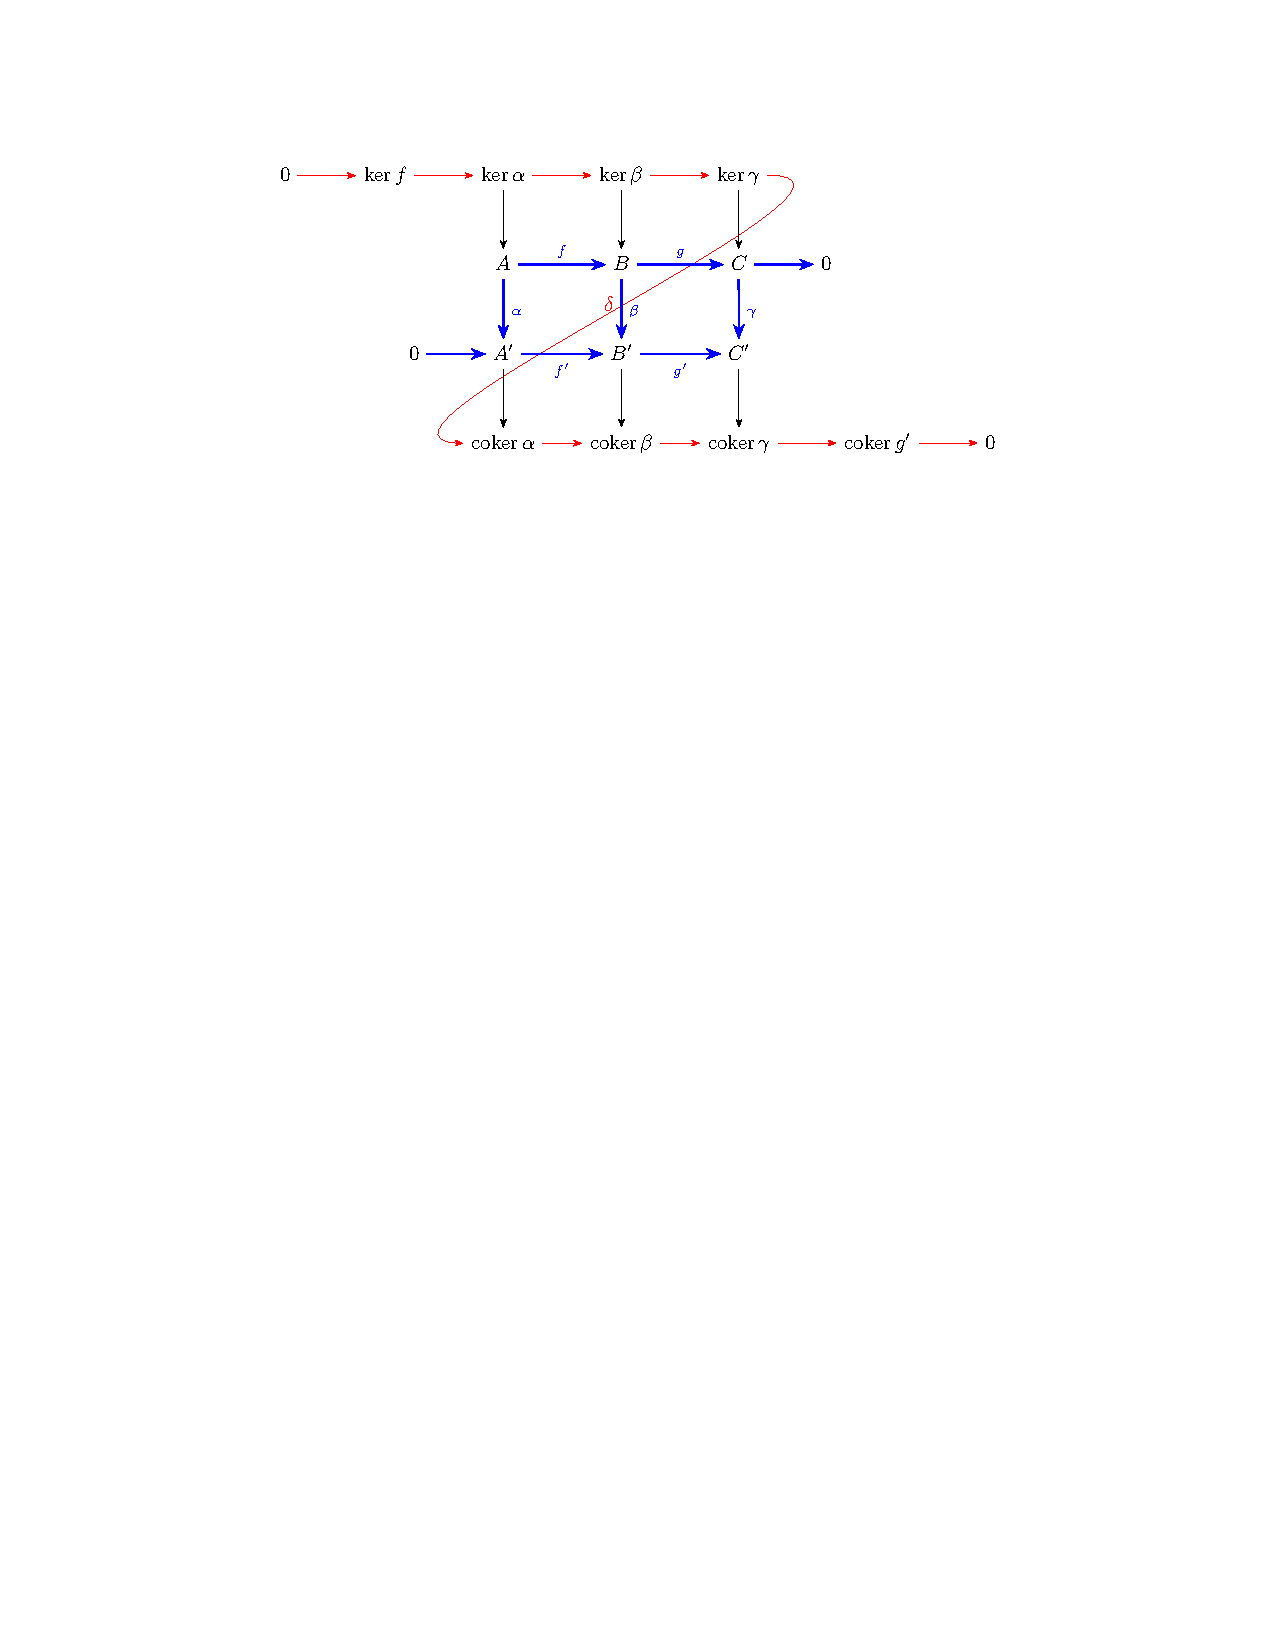
\includegraphics[width=0.8\textwidth]{pictures/snake.pdf}\]
the homomorphism $\delta$ is called the \textbf{connection homomorphism}.
\end{lemma}
\begin{proof}
First, let $c\in\ker\gamma$, We can construct elements of $A'$ as follows. Since $g$ is surjective, there exists an element $b\in B$ such that $g(b)=c$. We now move vertically down by $\beta$, and take $\beta(b)$. The commutativity $\gamma\circ g=g'\circ\beta$ shows that 
\[g'(\beta(b))=\gamma(g(b))=\gamma(c)=0\]
whence $\beta(b)$ is in the kernel of $g'$ in $B'$. By exactness, there exists an element $a'\in A'$ such that $f'(a)=\beta(b)$. We map $a$ into $\coker\alpha$ by the canonical projection, and still denote it by $a$.\par
In brief, we write
\[\delta(c)=a=f'^{-1}\circ\beta\circ g^{-1}(c)\]
\[\begin{tikzcd}
&&c\ar[d]\\
&b\ar[d,"\beta"]\ar[r,"g"]&c\ar[d,dashed,"\gamma"]\\
a\ar[d]\ar[r,"f'"]&\beta(b)\ar[r,dashed,"g'"]&0\\
a&&
\end{tikzcd}\]
We now verify that $\delta$ is well defined. First, $f'$ is injective by exactness, $a$ is uniquely determined by $\beta(b)$, hence by $b$. So the only verification is for $b$.\par
Suppose we choose a different $b'$ mapping to the same $c$: $g(b')=c=g(b)$. Then $b'-b\in\ker g$, and by exactness, $\im f=\ker g$, so there is $\ell\in A$ such that $\alpha(\ell)=b'-b$. It follows from the commutativity that
\[\beta(b'-b)=\beta(f(b'-b))=f'(\alpha(\ell))\]
Following our construction, $f'^{-1}(\beta(b'-b))=\alpha(\ell)$. But since the column is exact, the projection into $\coker\alpha$ kills $\alpha(\ell)$, hence taking $b'$ makes no difference to $\delta(c)$, that is, $\delta$ is well defined.
\[\begin{tikzcd}
\ell\ar[d,"\alpha"]\ar[r,"f"]&b'-b\ar[d,"\beta"]\ar[r,"g"]&0\\
\alpha(\ell)\ar[d]\ar[r,"f'"]&\beta(b'-b)&\\
0&&
\end{tikzcd}\]
Now we need to verify the exactness of the sequence. First we give the morphisms in the sequence
\[\begin{tikzcd}[column sep=tiny]
0\ar[r]&\ker f\ar[r,"i"]&\ker\alpha\ar[r,"f_*"]&\ker\beta\ar[r,"g_*"]&\ker\gamma\ar[r,"\delta"]&\coker\alpha\ar[r,"f'_*"]&\coker\beta\ar[r,"g'_*"]&\coker\gamma\ar[r,"j"]&\coker g'\ar[r]&0
\end{tikzcd}\]
We just define $f_*:=f|_{\ker\alpha}$, and similar for $g_*$, $f'_*,g'_*$. If $a\in\ker f$, then $f'(\alpha(a))=0$ by commutativity, and $\alpha(a)=0$ by injectvity of $f'$. This gives an inclusion $\ker f\to\ker\alpha$, which is our $i$. Similarly, if $c\in\im\gamma$, then there is an element $b\in B$ such that $\gamma(g(b))=c$ by the surjectivity of $g$. Then we see $c=g'(\beta(b))$ by commutativity, hence $c\in\im g'$. This gives $\im\gamma\sub\im g'$, and we have an induced quotient map $\coker\gamma\to\coker g'$. This is our $j$. By our definition, the exactness of two ends follows, now we begin to verify the rest.\par
Since $\ker f\sub\ker\alpha$, by our definition of $f_*$, the exactness at $\ker\alpha$ follows. Similar for the exactness of $\coker\gamma$. Since the top row is exact, $\im(f)=\ker(g)$. Ii follows that $g_*\circ f_*=0$, so $\im f_*\sub\ker g_*$. To verify the converse, assume $b\in\ker g_*$, that is, $b\in\ker\beta$ and $g(b)=0$. By exactness of $B$, there is $a\in A$ such that $f(a)=b$. We show that $a\in\ker\alpha$: in fact,
\[f'(\alpha(a))=\beta(f(a))=\beta(b)=0\]
Since $f'$ is injective, this means $\alpha(a)=0$, so $a\in\ker\alpha$. Thus $\ker g_*=\im f_*$, giving the exactness at $\ker\beta$.\par
The exactness at $\coker\beta$ arises similarly. Assume $b'+\im\beta\in\ker g'_*$, then $g'(b')\in\im\gamma$. By the surjectivity of $g$, $\exists b\in B$ such that $g'(b')=\gamma(g(b))=g'(\beta(b))$. Then $b'=\beta(b)+x$ with $x\in\ker g'$. By exactness, $x=f'(a')$ for some $a'\in A'$. Then it follows
\[b'+\im\gamma=\beta(b)+f'(a')+\im\beta=f'(a')\]
this shows $\ker g'_*\sub \im f'_*$, and the claim.\par
We verify the exactness about $\delta$. First, let $c=g(b)$ for some $b\in\ker\beta$. Since $\beta(b)=0$, by our definition of $\delta$, $\delta(c)=f'^{-1}(\beta(b))+\im\alpha=\im\alpha$. This gives $\im g_*\sub\ker\delta$. Conversely, if $\delta(c+\im\alpha)=\im\alpha$ for some $c\in C$, we get $\delta(c)\in\im\alpha$, hence $\delta(c)=\alpha(a)$ by some $a\in A$. By the construction of $\delta$, choose some $b\in B$ such that $g(b)=c$, then $f'^{-1}(\beta(b))=\delta(c)=\alpha(a)$ . It follows that
\[\beta(b)=f'(\alpha(a))=\beta(f(a))\]
and $b=f(a)+x$ for $x\in\ker\beta$. Applying $g$ we get $c=g(b)=g(f(a))+g(x)=g(x)$ since $g\circ f=0$. Since $x\in\ker\beta$, $g_*(x)=g(x)=c$. This gives $\ker\delta\sub\im g_*$, giving the exactness at $\ker\gamma$.
Finally, we deal with the exactness at $\coker\alpha$. Choose $a'+\im\alpha=\delta(c)$ for $c\in\ker\gamma$. Agian the definition of $\delta$: $f'(a')=f'(\delta(c))=\beta(b)$ for some $g(b)=c, b\in B$. This already gives 
\[f'_*(a'+\im\alpha)=f'(\delta(c))+\im\beta=\beta(b)+\im\beta=\im\beta\]
For the other direction, let $a'+\im\beta\in\ker f'_*$, that is, $f'(a')\in\im\beta$. So let $f'(a')=\beta(b), b\in B$, we observe that $a'=f'^{-1}\circ\beta(b)=f'^{-1}\circ\beta\circ g^{-1}(g(b))=\delta(g(b))$. This gives $\ker f'_*\sub\im\delta$, finishing the proof.
\end{proof}
\subsection{Exercise}
\begin{exercise}
Let $A$ be a local ring, and $f_1,\dots,f_r\in A$ be elements in $A$ generating a non-trivial ideal $I$ of $A$. Suppose $I$ is principal, show that $I=(f_i)$ for some $f_i$.
\end{exercise}
\begin{proof}
Let $I=(a)$ with $a\neq 0$ and $\m$ the unique maximal ideal of $A$. Then for every $f_i$ we have $f_i=k_ia$ for $k_i\in A$. Now consider the module $\m I$: we have $\m I\sub I$. If one of $k_i$ is a unit, then $I=(a_i)$ and we are done. So we assume this is not the case. Then, each $k_i$ is contained in $\m$, and hence $f_i=k_ia$ is in $\m I$, hence $I\sub\m I$. Now we have $\m I=I$, and by Nakayame's lemma we have $I=0$, which is contradiction.
\end{proof}
\begin{exercise}
Let $A[X]$ be the ring of polynomials in one indeterminate over a ring A. Prove that $A[X]$ is a flat $A$-algebra.
\end{exercise}
\begin{proof}
We have
\[A[X]=\bigoplus_{i\in\N}(x^n)\]
Each $(x^n)$ is free, hence flat, so $A[X]$ is flat.
\end{proof}
\begin{exercise}
For any $A$-module, let $M[X]$ denote the set of all polynomials in $x$ with coefficients in $M$, prove that
\[A[X]\otimes_AM\cong (A\otimes_AM)[X]\cong M[X].\]
\end{exercise}
\begin{exercise}
Let 
\[\begin{tikzcd}
0\ar[r]&L\ar[r]&M\ar[r]&N\ar[r]&0
\end{tikzcd}\]
be an exact sequence of $A$-modules. If $L$ and $N$ are finitely generated, then so is $M$.
\end{exercise}
\begin{proof}
We have $M\sub L+N$ if we identify this sequence as a projection.
\end{proof}
\begin{exercise}
If $M$ is a finitely generated $A$-module and $f:M\to M$ is a surjective homomorphism, then $f$ is an isomorphism.
\end{exercise}
\begin{proof}
Define a $A[X]$-module structure on $M$ via $x\cdot m:=f(m)$. Let $I:=(x)$, we claim that $IM=M$: In fact, since $f$ is surjective, for each $m\in M$ there is $n\in M$ such that $x\cdot n=f(n)=m$, so $m\in IM$. Now by \cref{finite module IM=M} there exists $g\in I$ such that $(1+g)M=0$. By the definition of $I$, we can write $g(x)=xh(x)$.\par
Now we prove $f$ is injective. Let $m\in M$ be such that $f(m)=0$. Then
\[0=(1+xh(x))\cdot m=m+h(x)\cdot f(m)=m+0=m.\]
This finishes the proof.
\end{proof}
\begin{exercise}\label{module directed limit}
Let $\mathcal{M}=(M_i,\mu_i)$ be a directed system directed by some set $I$. We shall construct an $A$-module $M$ called the direct limit of the direct system $M$. Let $C$ be the direct sum of the $M_i$ and identify each module $M_i$ with its canonical image in $C$. Let $D$ be the submodule of $C$ generated by all elements of the form $x_i-\mu_{ij}(x_i)$ where $i\leq j$ and $x_i\in M_i$. Let $M=C/D$, let $\mu:C\to M$ be the projection and let $\mu_i$ be the restriction of $\mu$ to $M_i$. Then clearly $\mu_j=\mu_{ij}\mu_i$. Show that every element of $M=\rlim M_i$ can be written in the form $\mu_i(x_i)$ for some $i\in I$ and some $x_i\in M_i$. Show also that if $\mu_i(x_i)=0$ then there exists $j\geq i$ such that $\mu_{ij}(x_i)=0$ in $M_j$.
\end{exercise}
\begin{proof}
For the first claim, $x\in C$ has a representative of the form $x=\sum_{j\in J}x_j$ for some finite subset $J$. Then we can get $i\in I$ such that $i\geq j$ for all $j\in J$. So
\[x=\mu\Big(\sum_{j\in J}x_j\Big)=\sum_{j\in J}\mu_j(x_j)=\sum_{j\in J}\mu_i\mu_{ji}(x_j)=\mu_i\Big(\sum_{j\in J}\mu_{ji}(x_j)\Big)\]
Let $x_i=\sum\mu_{ji}(x_j)$ we get the claim.\par
For the second claim, suppose $\mu_i(x_i)=0$ for some $i\in I$. Then, $x_i\in M_i\cap D$ is a finite sum
\[x_i=\sum_{\ell}(y_{j_\ell}-\mu_{j_{\ell}k_{\ell}}(y_{j_\ell}))\]
for some finite subset $J$ of $I$, and $y_{j_\ell}\in M_{j_\ell}$ for each $j\in J$ with $j_\ell\leq k_\ell$. Now, there exists $l\in I$ such that $l\geq k_\ell$ for all $k_\ell\in J\cup\{i\}$. Let $\pi_a:x\to M_a$ be the projectin, then we have
\[\pi_a=\sum_{j_\ell =a}y_{j_\ell}-\sum_{k_\ell=a}\mu_{j_\ell k_\ell}(y_{j_\ell}).\]
Hence
\[\mu_{al}(\pi_a(x_i))=\sum_{j_\ell =a}\mu_{al}(y_{j_\ell})-\sum_{k_\ell=a}\mu_{j_\ell l}(y_{j_\ell})\]
It follows that
\begin{align*}
\sum_a\mu_{al}\pi_a(x_i)&=\sum_a\Big(\sum_{j_\ell =a}\mu_{al}(y_{j_\ell})-\sum_{k_\ell=a}\mu_{j_\ell l}(y_{j_\ell})\Big)\\
&=\sum_{\ell}\sum_{a=j_\ell}\mu_{al}(y_{j_\ell})-\sum_{\ell}\sum_{a=k_\ell}\mu_{j_\ell l}(y_{j_\ell})\\
&=\sum_{\ell}\mu_{j_\ell l}(y_{j_\ell})-\sum_{\ell}\mu_{j_\ell l}(y_{j_\ell})=0
\end{align*}
Since $x_i\in M_i$, the left sum is $\mu_{il}(x_i)$, and we get $\mu_{il}(x_i)=0$.
\end{proof}
\begin{exercise}\label{module directed limit exactness}
Let $I$ be a directed set, and let $(A_i,\alpha_{ij})$, $(B_i,\beta_{ij})$, and $(C_i,\gamma_{ij})$ be direct systems of $A$-modules over $I$. If $r_i:A_i\to B_i$ and $s_i:B_i\to C_i$ are morphisms of direct systems, and if
\[\begin{tikzcd}
0\ar[r]&A_i\ar[r,"r_i"]&B_i\ar[r,"s_i"]&C_i\ar[r]&0
\end{tikzcd}\]
is exact for each $i\in I$, then there is an exact sequence
\[\begin{tikzcd}
0\ar[r]&\rlim A_i\ar[r,"r"]&\rlim B_i\ar[r,"s"]&\rlim C_i\ar[r]&0
\end{tikzcd}\]
where $r=\vec{r}_i$, $s=\vec{s}_i$. Consequently, filtered colimits commute with homology in $A$-$\mathsf{Mod}$.
\end{exercise}
\begin{proof}
Since direct limit is a left adjoint functor, it is right-exact. Hence we only need to prove $r$ is injective. Suppose that $r(x)=0$, where $x\in\rlim A_i$. Since the index set $I$ is
directed, allows us to write $x=\alpha_i(a_i)$, where $\alpha_i:A_i\to\bigoplus A_i$ is projection, similar for $\beta_i$. Now, be definition we have
\[r(x)=\beta_ir_i(a_i).\]
so $\beta_ir_i(a_i)=0$. By \cref{module directed limit}, there is a $j\geq i$ such that $\beta_ir_i(a_i)=\beta_{ij}r_i(a_i)=0$. Since $r_i$ is a map of direct systems, we have
\[r_j\alpha_{ij}=\beta_{ij}r_i\]
Thus $r_j\alpha_{ij}(a_i)=0$, and by the injectivity of $r_j$, we conclude $\alpha_{ij}(a_i)=0$, since we have
\[x=\alpha_i(a_i)=\alpha_j\alpha_{ij}(a_i)\]
we conclude $x=0$. 
\end{proof}
\begin{exercise}
Let $(M_i)_{i\in I}$ be a family of submodules of an $A$-module, such that for each pair of indices $i$, $j$ in $I$ there exists $k\in I$ such that $M_i+M_j\sub M_k$. Define $i\leq j$ to mean $M_i\sub M_j$ and let $\mu_{ij}:M_i\to M_j$ be the embedding of $M_i$ in $M_j$. Show that
\[\rlim M_i=\sum M_i=\bigcup_iM_i.\]
In particular, any $A$-module is the direct limit of its finitely generated submodules.
\end{exercise}
\begin{proof}
We can easily check that $\bigcup_iM_i$ is a module and satisfies that universal property of $\rlim M_i$. And since it has the same discription as $\sum M_i$, we get the equality.
\end{proof}
\begin{exercise}
Let $\mathcal{M}=(M_i,\mu_{ij})$, $\mathcal{N}=(N_i,\nu_{ij})$ be direct systems of $A$-modules over the same directed set. Let $M,N$ be the direct limits and $\mu_i:M\to M$, $\nu_i:N_i\to N$ the associated homomorphisms.\par
A homomorphism $\Phi:\mathcal{M}\to\mathcal{N}$ is by definition a family of $A$-module homomorphisms $\phi_i:M_i\to N_i$, such that $\phi_i\circ\mu_{ij}=\nu_{ij}$ whenever $i\leq j$. Show that $\Phi$ defines a unique homomorphism $\phi=\rlim\phi_i:M\to N$ such that $\phi\circ\mu_i=\nu_i$ for all $i\in I$.
\end{exercise}
\begin{exercise}\label{ring direct limit zero iff one zero}
Consider a direct limit of rings $A=\rlim A_i$, prove that $\rlim A=0$ if and only if $A_i=0$ for some $i$.
\end{exercise}
\begin{proof}
If $A=0$, then in particular $0=1$. By exercise~\ref{module directed limit}, for fixed $i$, there exists $j\in I$ such that $\mu_{ij}(a)=0$. Since $\mu_{ij}$ is also a ring homomorphism from $A_i$ to $A_j$, this implies that $1=0$ in $A_j$ and hence $A_j=0$.
\end{proof}
\begin{exercise}
Let $(A_i,\mu_i)$ be a direct system of rings and let $\n(A_i)$ be the nilradical of $A_i$. Show that $\rlim \n(A_i)$ is the nilradical of $\rlim A_i$. If each $A_i$ is an integral domain, then $\rlim A_i$ is an integral domain.
\end{exercise}
\begin{proof}
Let $a$ be a nilpotent element of $A$. Then $\exists n\in\N$ such that $a^n=0$. By \cref{module directed limit}, $a=\mu_i(x)$ thus $0=a^n=\mu_i(x^n)$. By \cref{module directed limit}, $\mu_i(x^n)=0$ implies $\exists j\geq i$ such that $\mu_{ij}(x^n)=0$. Hence, $\mu_{ij}(x)$ is in the nilradical of $A_j$, and
\[\mu_j(\mu_{ij}(x))=\mu_i(x)=a\]
Hence $a\in\rlim \n(A_i)$.\par
Conversely, if $a\in\rlim \n(A_i)$, then by \cref{module directed limit}, there is $x_i\in M_i$ such that $\mu_i(x_i)=a$. Then 
\[a^n=\mu_i(x_i^n)=0\]
so there is $j\geq i$ such that $\mu_{ij}(x_i^n)=0=\mu_{ij}(x_i)^n$. This means $\mu_{ij}(x_i)$ is in $\n(A_j)$. Since
\[\mu_j(\mu_{ij}(x_i))=\mu_i(x)=a,\]
we see $a$ is nilpotent in $A$.
\end{proof}
\section{Flat modules}
\subsection{\texorpdfstring{$M$}{M}-flat modules}
Let $A$ be a ring, $E$ and $M$ $A$-modules. Then $E$ is said to be \textbf{flat for $\bm{M}$} (or \textbf{$\bm{M}$-flat}) if, for every $A$-module $N$ and every injective homomorphism $\phi:M'\to M$, the homomorphism $1\otimes v:E\otimes_AM'\to E\otimes_AM$ is injective.
\begin{lemma}\label{module flat iff finite submodule}
For an $A$-module $E$ to be $M$-flat, it is necessary and sufficient that for every finitely generated submodule $N$ of $M$ the canonical homomorphism $1\otimes v:E\otimes_AN\to E\otimes_AM$ is injective.
\end{lemma}
\begin{proof}
Suppose that this condition holds and let $N$ be any submodule of $M$. Suppose that the canonical image in $E\otimes_AM$ of an element $z=\sum_ix_i\otimes y_i\in E\otimes M$ is zero and let $M'$ be the finitely generated submodule of $N$ generated by the $y_i$. As by hypothesis the composition map
\[E\otimes_AM'\to E\otimes_AN\to E\otimes_AM\]
is injective, the sum $z'=\sum_ix_i\otimes y_i$ considered as an element of $E\otimes_AM'$, is zero. Since $z$ is the image of $z'$, we have $z=0$, whence the lemma.
\end{proof}
\begin{lemma}\label{module submodule quotient flat}
Let $E$ be an $A$-module and $M$ an $A$-module such that $E$ is $M$-flat. If $N$ is either a submodule or a quotient module of $M$, then $E$ is $N$-flat.
\end{lemma}
\begin{proof}
The case in which $N$ is a submodule is easy, as, if $N'$ is a submodule of $N$, the composite homomorphism
\[E\otimes_AN'\to E\otimes_AN\to E\otimes_AM\]
is injective, hence so is $E\otimes_AN'\to E\otimes_AN$. Suppose then that $N$ is a quotient module of $M$, that is there exists an exact sequence
\[\begin{tikzcd}
0\ar[r]&R\ar[r,"i"]&M\ar[r,"\pi"]&N\ar[r]&0
\end{tikzcd}\]
Let $N'$ be a submodule of $N$ and $M'=\pi^{-1}(N')$. Let $\iota'$ denote the mapping of $R$ to $M'$ with the same graph as $\iota$, $\pi'$ the surjection $M'\to N'$ with the same graph as the restriction of $\pi$ to $M'$, and $\phi$, $\psi$, $\gamma$ the canonical injections. The the folloiwng diagram 
\[\begin{tikzcd}
0\ar[r]&R\ar[d,"\phi"]\ar[r,"\iota'"]&M'\ar[d,"\psi"]\ar[r,"\pi'"]&N'\ar[d,"\gamma"]\ar[r]&0\\
0\ar[r]&R\ar[r,"\iota"]&M\ar[r,"\pi"]&N\ar[r]&0
\end{tikzcd}\]
is commutative and its rows are exact. Tensoring with $E$, since $E$ is $M$-flat, we get the following diagram
\[\begin{tikzcd}
&E\otimes_AR\ar[d,"1\otimes\phi"]\ar[r,"1\otimes\iota'"]&E\otimes_AM'\ar[d,"1\otimes\psi"]\ar[r,"1\otimes\pi'"]&E\otimes_AN'\ar[d,"1\otimes\gamma"]\ar[r]&0\\
0\ar[r]&E\otimes_AR\ar[r,"1\otimes\iota"]&E\otimes_AM\ar[r,"1\otimes\pi"]&E\otimes_AN\ar[r]&0
\end{tikzcd}\]
with row exact. Now since $1\otimes\phi$ is surjective and $1\otimes\psi$ is injective, by snake lemma we see $1\otimes\gamma$ is injective, whence the claim. 
\end{proof}
\begin{lemma}\label{module flat and direct sum}
Let $(M_i)_{i\in I}$ be a family of $A$-modules, $M=\bigoplus_iM_i$ their direct sum and $E$ an $A$-module. If, for all $i\in I$, $E$ is flat for $M_i$, then $E$ is flat for $M$.
\end{lemma}
\begin{proof}
Suppose first that $I=\{1,2\}$, and let $M'$ be a submodule of $M=M_1\oplus M_2$, $M_1$ and $M_2$ being canonically identified with submodules of $M$. Denote by $M_1'$ the intersection $M'\cap M_1$ and by $M_2'$ the image of $M'$ in $M_2$ under the canonical projection $\pi$ of $M$ onto $M_2$. We have a diagram
\[\begin{tikzcd}
0\ar[r]&M_1'\ar[r,"\iota'"]\ar[d,"\phi"]&M'\ar[r,"\pi'"]\ar[d,"\psi"]&M_2'\ar[r]\ar[d,"\eta"]&0\\
0\ar[r]&M_1\ar[r,"\iota"]&M\ar[r,"\pi"]&M_2\ar[r]&0
\end{tikzcd}\]
where $\iota$, $\iota'$ are the canonical injections and $\pi'$ is the mapping with the same graph as the restriction of $\pi$ to $M'$, which is surjective. It is immediately verified that this diagram is commutative and that its rows are exact.
\[\begin{tikzcd}
&E\otimes_AM_1'\ar[r,"1\otimes\iota'"]\ar[d,"1\otimes\phi"]&E\otimes_AM'\ar[r,"1\otimes\pi'"]\ar[d,"1\otimes\psi"]&E\otimes_AM_2'\ar[r]\ar[d,"1\otimes\eta"]&0\\
0\ar[r]&E\otimes_AM_1\ar[r,"1\otimes\iota"]&E\otimes_AM\ar[r,"1\otimes\pi"]&E\otimes_AM_2\ar[r]&0
\end{tikzcd}\]
By hypotheses the two rows of this diagram are exact. As $E$ is flat for $M_1$ and $M_2$, $1\otimes\phi$ and $1\otimes\eta$ are injective. The snake lemma then shows that $1\otimes\psi$ is injective and consequently $E$ is $M$-flat.\par
If $I$ is a finite set with $n$ elements, the lemma follows by induction on $n$. In the general case, let $M'$ be a finitely generated submodule of $M$. Then there exists a finite subset $J$ of the indexing set $I$ such that $M'$ is contained in the direct sum $M^J=\bigoplus_{i\in J}M_j$. By the finite case $E$ is flat for $M^J$. The canonical homomorphism $E\otimes_AM'\to E\otimes_AM^J$ is therefore injective. On the other hand, as $M^J$ is a direct factor of $M$, the canonical homomorphism $E\otimes_AM^J\to E\otimes_AM$ is injective. Taking the composition, it follows that $E\otimes_AM^J\to E\otimes_AM$ is injective and $E$ is flat for $M$ by \cref{module flat iff finite submodule}.
\end{proof}
\subsection{Flat modules}
\begin{proposition}\label{module flat iff flat for A}
Let $E$ be an $A$-module. The following three properties are equivalent:
\begin{itemize}
\item[(\rmnum{1})] $E$ is flat for $A$ (in other words, for every ideal $\a$ of $A$, the canonical homomorphism $E\otimes_A\a\to E\otimes_AA$ is injective).
\item[(\rmnum{2})] $E$ is $M$-flat for every $A$-module $M$.
\item[(\rmnum{3})] The functor $\otimes_AE$ is exact, that is, $E$ is flat.
\end{itemize}
\end{proposition}
\begin{proof}
It is immediate that (\rmnum{2}) is equivalent to (\rmnum{3}) and (\rmnum{2}) implies (\rmnum{1}). Conversely, if (\rmnum{1}) holds, then by \cref{module flat and direct sum}, $E$ is fiat for every flee left $A$-module. As every $A$-module is isomorphic to a quotient of a free module, it follows from \cref{module submodule quotient flat} that $E$ is flat for $M$.
\end{proof}
\begin{remark}By \cref{module flat iff finite submodule}, for an $A$-module $E$ to be flat, it is necessary and sufficient that, for every finitely generated ideal $\a$ of $A$, the canonical mapping $E\otimes_A\a$ with image $E\a$ be injective.
\end{remark}
\begin{proposition}\label{module direct sum flat iff}
Let $(E_i)_{i\in I}$ be a family of $A$-modules. For $E=\bigoplus_iE_i$ to be flat, it is necessary and sufficient that each of the $E_i$ be flat.
\end{proposition}
\begin{proof}
Let $M'\to M$ be an injective $A$-module homomorphism. For the direct sum homomorphism
\[\bigoplus_{i\in I}(E_i\otimes_AM)\to\bigoplus_{i\in I}(E_i\otimes_AM)\]
to be exact, it is necessary and sufficient that each of the homomorphisms $E_i\otimes_AM'\to E_i\otimes_AM$ be so, which proves the claim since $\bigoplus_{i\in I}(E_i\otimes_AM)$ is canonically identified with $E\otimes_AM$.
\end{proof}
\begin{proposition}\label{module flat direct limit}
Let $I$ be an ordered set and $(E_\alpha,f_{\beta\alpha})$ a direct system of $A$-modules. If each of the $E_\alpha$ is flat, then $E=\rlim E_\alpha$ is flat.
\end{proposition}
\begin{proof}
By hypothesis each of the sequences $0\to E_\alpha\otimes_AM'\to E_\alpha\otimes_AM$ is exact; so then is the sequence $0\to E\otimes_AM'\to E\otimes_AM$ since taking the direct limit commutes with tensor products and preserves exactness.
\end{proof}
\begin{example}
\mbox{}
\begin{itemize}
\item[(a)] For any ring $A$, $A$ is clearly a flat $A$-module. Then it follows from \cref{module direct sum flat iff} that every free $A$-module, and more generally every projective $A$-module, is a flat $A$-module.
\item[(b)] If $A$ is a semisimple ring, every $A$-module $E$ is semisimple and hence a direct sum of simple modules. As each of these latter is isomorphic to a direct factor of $A$, $E$ is projective and therefore flat.
\item[(c)] Let $a\in A$ be such that the map $a_A:x\mapsto ax$ on $A$ is injective ($a$ is not a zero divisor). If $E$ is a flat $A$-module, then the homothety $a_E$ is injective. In particular, if $A$ is integral, any flat $A$-module is torsion free. Conversely, if $A$ is a PID, then any torsion free $A$-module is flat: infact, if the $A$-module $E$ is torsion-free, any finitely generated submodule of $E$ is free, and $E$ is the union of these flat submodules, hence flat (\cref{module flat direct limit}).
\end{itemize}
\end{example}
\begin{proposition}\label{module flat and torsion}
Let $A$ be a ring and $E$ an $A$-module.
\begin{itemize}
\item[(a)] Suppose that $E$ is flat. For every element $a$ of $A$ which is not a divisor of $0$, the relations $x\in E$, $ax=0$ imply $x=0$. 
\item[(b)] Suppose that $A$ is an integral domain in which every finitely generated ideal is principal. Then for $E$ to be flat it is necessary and sufficient that $E$ be torsion-free.
\end{itemize}
\end{proposition}
\begin{proof}
We prove (a). Let $v:A\to A$ be the $A$-module homomorphism $t\mapsto at$. The hypothesis implies that $v$ is injective. As $E$ is flat, the homomorphism $1_E\otimes v:E\otimes_AA\to E\otimes_AA$ is also injective. When $E\otimes_AA$ is canonically identified with $E$, $1_E\otimes v$ becomes the endomorphism $x\mapsto ax$ of $E$. Thus the relation $ax=0$ implies $x=0$.\par
We prove (b). By (a), if $E$ is flat, $E$ is torsion-free. Conversely, let $E$ be a torsion-free $A$-module and let $\a$ be a nonzero finitely generated ideal of $A$. By hypothesis $\a=Aa$ for some nonzero $a\in A$ and $t\mapsto at$ is then an isomorphism $v$ of $A$ onto $\a$. Using $i$ to denote the canonical injection $\a\to A$, $i\circ v$ is the homothety with ratio $a$ on $E$ and is injective since $E$ is assumed to be torsion-free. Then $1_E\otimes(i\circ v)=(1_E\otimes i)\circ(1_E\otimes v)$. As $1_E\otimes v$ is an isomorphism, $1_E\otimes i$ is injective, which completes the proof.
\end{proof}
\begin{proposition}\label{module flat iff quotient of flat module}
Let $E$ be an $A$-module. The three following properties are equivalent:
\begin{itemize}
\item[(\rmnum{1})] $E$ is flat.
\item[(\rmnum{2})] For every exact sequence of $A$-modules of the form
\begin{equation}\label{module flat iff quotient of flat module-1}
\begin{tikzcd}
0\ar[r]&G\ar[r,"\phi"]&H\ar[r,"\psi"]&E\ar[r]&0 
\end{tikzcd}
\end{equation}
and every $A$-module $F$, the sequence
\begin{equation}\label{module flat iff quotient of flat module-2}
\begin{tikzcd}
0\ar[r]&G\otimes_AF\ar[r,"\phi\otimes 1"]&H\ar[r,"\psi\otimes 1"]&E\otimes_AF\ar[r]&0 
\end{tikzcd}
\end{equation}
sexact.
\item[(\rmnum{3})] There exists an exact sequence $(\ref{module flat iff quotient of flat module-1})$, where $H$ is flat, such that the sequence $(\ref{module flat iff quotient of flat module-2})$ is is exact for every $A$-module $F$ of the form $A/\a$, where $\a$ is a finitely generated ideal of $A$.
\end{itemize}
\end{proposition}
\begin{proof}
The $A$-module $F$ is isomorphic to a quotient of a free module. In other words, we have an exact sequence $\begin{tikzcd}[column sep=15pt]
0\ar[r]&R\ar[r,"\iota"]&L\ar[r,"\pi"]&F\ar[r]&0\end{tikzcd}$ where $L$ is free. Consider the diagram
\begin{equation}\label{module flat iff quotient of flat module-3}
\begin{tikzcd}[column sep=20pt,row sep=20pt]
&G\otimes_AR\ar[r,"\phi\otimes 1_R"]\ar[d,"1_G\otimes\iota"]&H\otimes_AR\ar[r,"\psi\otimes 1_R"]\ar[d,"1_H\otimes\iota"]&E\otimes_AR\ar[r]\ar[d,"1_E\otimes\iota"]&0\\
0\ar[r]&G\otimes_AL\ar[r,"\phi\otimes 1_L"]\ar[d,"1_G\otimes\pi"]&H\otimes_AL\ar[r,"\psi\otimes 1_L"]\ar[d,"1_H\otimes\pi"]&E\otimes_AL\ar[r]\ar[d,"1_F\otimes\pi"]&0\\
&G\otimes_AF\ar[r,"\phi\otimes 1_F"]\ar[d]&H\otimes_AF\ar[r,"\phi\otimes 1_F"]\ar[d]&E\otimes_AF\ar[r]\ar[d]&0\\
&0&0&0
\end{tikzcd}
\end{equation}
It follows immediately that this diagram is commutative, and its rows and columns are exact. Apply the snake lemma to the first two rows, we get the following exact sequence
\begin{equation}\label{module flat iff quotient of flat module-4}
\begin{tikzcd}
\ker(1_H\otimes\iota)\ar[r]&\ker(1_E\otimes\iota)\ar[r,"\delta"]&G\otimes_AF\ar[r,"\phi\otimes 1_F"]&H\otimes_AF
\end{tikzcd}
\end{equation}
Now if $E$ is flat, then $1_E\otimes\iota$ is injective, and the exact sequence shows that $\phi\otimes 1_F$ is injective, hence the sequence $(\ref{module flat iff quotient of flat module-2})$ is exact.\par
As (\rmnum{2}) obviously implies (\rmnum{3}), it remains to prove that (\rmnum{3}) implies (\rmnum{1}). Consider the diagram $(\ref{module flat iff quotient of flat module-3})$ in the case $R=\a$, $L=A$, $F=A/\a$ and apply the exact sequence $(\ref{module flat iff quotient of flat module-4})$. By hypothesis $\phi\otimes 1_F$ is injective, so $\im\delta=0$. Moreover, as $H$ is exact, we see $\ker(1_H\otimes\iota)=0$, whence $\ker(1_E\otimes\iota)=0$ and $E$ is flat.
\end{proof}
\begin{proposition}\label{module exact flat and exact sequence}
Let $\begin{tikzcd}[column sep=15pt,row sep=15pt]0\ar[r]&E_1\ar[r,"\phi"]&E_2\ar[r,"\psi"]&E_3\ar[r]&0\end{tikzcd}$ be an exact sequence of $A$-modules. Suppose $E_3$ is flat. Then, for $E_2$ to be flat it is necessary and sufficient that $E_1$ be flat.
\end{proposition}
\begin{proof}
Let $\eta:F'\to F$ be an injective homomorphism of $A$-modules. Consider the diagram
\[\begin{tikzcd}
0\ar[r]&E_1\otimes_AF'\ar[r,"\phi\otimes 1_{F'}"]\ar[d,"1_{E_1}\otimes\eta"]&E_2\otimes_AF'\ar[r,"\psi\otimes 1_{F'}"]\ar[d,"1_{E_2}\otimes\eta"]&E_3\otimes_AF'\ar[r]\ar[d,"1_{E_3}\otimes\eta"]&0\\
0\ar[r]&E_1\otimes_AF\ar[r,"\phi\otimes 1_{F}"]&E_2\otimes_AF\ar[r,"\psi\otimes 1_{F}"]&E_3\otimes_AF\ar[r]&0
\end{tikzcd}\]
It is commutative and its rows are exact by \cref{module flat iff quotient of flat module}. Since $E_3$ is flat, we know $1_{E_3}\otimes\eta$ is injective. Now snake lemma gives the claim.
\end{proof}
Let $E$ and $F$ be $A$-modules. Every element of $E\otimes_AF$ can be written in at least one way in the form $z=\sum_{i=1}^{n}e_i\otimes f_i$ where $e_i\in E$ and $f_i\in F$. The following lemma gives a condition under which this sum is zero:
\begin{lemma}\label{module tensor zero iff}
Let $(f_i)_{i\in I}$ be a family of generators of $F$ and $(e_i)_{i\in I}$ a family of elements of $E$ of finite support. For $\sum_{i\in I}e_i\otimes f_i=0$, it is necessary and sufficient that there exist a finite set $J$, a family $(x_j)_{j\in J}$ of elements of $E$ and a family $(a_{ji})_{j\in J,i\in I}$ of elements of $A$ with the following properties:
\begin{itemize}
\item[(a)] the family $(a_{ji})$ has finite support;
\item[(b)] $\sum_{i\in I}a_{ji}f_i=0$ for all $j\in J$;
\item[(c)] $e_i=\sum_{j\in J}a_{ji}x_j$ for all $i\in I$.
\end{itemize}
\end{lemma}
\begin{proof}
Consider the free $A$-module $A^{\oplus I}$, its canonical basis $(u_i)$ and the homomorphism $g:A^{\oplus I}\to F$ such that $g(u_i)=f_i$ for all $i\in I$. Denoting by $R$ the kernel of $g$, we have (since the $f_i$ generate $F$) an exact sequence
\[\begin{tikzcd}
R\ar[r,"\iota"]&A^{\oplus I}\ar[r,"g"]&F\ar[r]&0
\end{tikzcd}\]
wherc $\iota$ denotes the canonical injection. We derive from this the exact sequence
\begin{equation}\label{module tensor zero iff-1}
\begin{tikzcd}
E\otimes_AR\ar[r]&E\otimes_AA^{\oplus I}\ar[r,"1\otimes g"]&E\otimes_AF\ar[r]&0
\end{tikzcd}
\end{equation}
Now, $E\otimes_AA^{\oplus I}$ is canonically identified with $E^{\oplus I}$ a family $e=(e_i)\in E^{\oplus I}$ being identified with $\sum_{i\in I}e_i\otimes u_i$. For such a family to belong to the kernel of $1_E\otimes g$, it is necessary and sufficient that $\sum_{i\in I}e_i\otimes f_i=0$ in $E\otimes_AF$. Taking account of the exact sequence $(\ref{module tensor zero iff-1})$, this is equivalent to saying that $e$ belongs to the image of $1_E\otimes\iota$, in other words there is a relation of the form
\begin{equation}\label{module tensor zero iff-2}
\sum_{i\in I}e_i\otimes u_i=\sum_{j\in J}x_j\otimes\iota(r_j)
\end{equation}
where $x_i\in E$, $r_i\in R$ and $J$ is finite. Writing $\iota(r_i)=\sum_{i\in I}a_{ji}u_i$, the hypothesis $r_j\in R$ implies the relation $\sum_{i\in I}a_{ji}f_i=0$ for all $j\in J$. On the other hand the relation $(\ref{module tensor zero iff-2})$ implies $e_i=\sum_{j\in J}a_{ji}x_j$ for all $i\in I$ (\cref{*}), which completes the proof.
\end{proof}
\begin{proposition}\label{module F-flat iff linear relation}
For $E$ to be $F$-flat, it it necessary and sufficient that the following condition be satisfied:
\begin{itemize}
\item[(R)] If $(e_i)_{i\in I}$ and $(f_i)_{i\in I}$ are two finite families of elements of $E$ and $F$ respectively such that $\sum_{i\in I}e_i\otimes f_i=0$ in $E\otimes_AF$, there exists a finite set $J$, a family $(x_j)_{j\in J}$ of elements of $E$ and a family $(a_{ji})_{j\in J,i\in I}$ of elements of $A$, with the following properties:
\begin{itemize}
\item[(a)] $\sum_{i\in I}a_{ji}f_i=0$ for all $j\in J$. 
\item[(b)] $e_i=\sum_{j\in J}a_{ji}x_j$ for all $i\in I$.
\end{itemize} 
\end{itemize}
\end{proposition}
\begin{proof}
Suppose that $E$ is $F$-flat. Let $(e_i)$ and $(f_i)$ be finite families of elements such that $\sum_{i\in I}e_i\otimes f_i=0$ in $E\otimes_AF$, and let $F'$ be the submodule of $F$ generated by the $f_i$. Since the canonical mapping $E\otimes_AF'\to E\otimes_AF$ is injective, we have also $\sum_{i\in I}e_i\otimes f_i=0$ in $E\otimes_AF'$ and \cref{module tensor zero iff} can then be applied to $E$ and $F'$. Thus families $(x_j)$ and $(a_{ji})$ are obtained satisfying the conditions of (R).\par
Conversely, suppose that condition (R) holds. Let $F'$ be a submodule of $F$ and let $y=\sum_{i\in I}e_i\otimes f_i$ be an element of the kernel of the canonical mapping $E\otimes_AF'\to E\otimes_AF$. Since (R) holds, there exist families $(x_j)$ and $(a_{ji})$ satisfying conditions (a) and (b). We conclude that, in $E\otimes_AF$,
\[y=\sum_{i,j}a_{ji}x_j\otimes f_i=\sum_{j\in J}(x_j\otimes\sum_{i\in I}a_{ji}f_i)=0\]
hence the map $E\otimes F'\to E\otimes F$ is injective.
\end{proof}
\begin{corollary}
For an $A$-module $E$ to be flat, it is necessary and sufficient that the following condition hold:
\begin{enumerate}[leftmargin=30pt]
\item[(RP)] Every solution $\bm{y}\in M^n$ of a linear equation $P\bm{y}=0$ with $P\in\mathcal{M}_{mn}(A)$ is a linear combination $\bm{y}=Q\bm{x}$, where $Q\in\mathcal{M}_{nk}(A)$, $\bm{x}\in M^k$ and $PQ=0$.
\end{enumerate}
\end{corollary}
\subsection{Intersection properties}
\begin{lemma}\label{module tensor intersection lemma}
Let $E$ be an $A$-module, $F$ an $A$-module and $F_1$, $F_2$ two submodule of $F$ such that $F=F_1+F_2$. Then the intersection of the canonical images of $E\otimes F_1$ and $E\otimes F_2$ in $E\otimes F$ is equal to the canonical image of $E\otimes(F_1\cap F_2)$.
\end{lemma}
\begin{proof}
Consider the diagram
\[\begin{tikzcd}[column sep=20pt,row sep=20pt]
0\ar[r]&F_1\cap F_2\ar[r]\ar[d]&F_1\ar[r]\ar[d]&F_1/(F_1\cap F_2)\ar[r]\ar[d,"\eta"]&0\\
0\ar[r]&F_2\ar[r]&F_1+F_2\ar[r]&(F_1+F_2)/F_2\ar[r]&0
\end{tikzcd}\]
where the unspecified arrows are the canonical injections and surjections and $\eta$ is the canonical isomorphism. This diagram is commutative and its rows are exact. We derive (since $F=F_1+F_2)$ a commutative diagram
\[\begin{tikzcd}[column sep=20pt,row sep=20pt]
E\otimes(F_1\cap F_2)\ar[r]\ar[d]&E\otimes F_1\ar[r]\ar[d]&E\otimes(F_1/(F_1\cap F_2))\ar[r]\ar[d,"1_E\otimes\eta"]&0\\
E\otimes F_2\ar[r]&E\otimes F\ar[r]&E\otimes((F_1+F_2)/F_2)\ar[r]&0
\end{tikzcd}\]
The rows of this diagram are exact and $1_E\otimes\eta$ is an isomorphism. A simple diagram chasing shows the claim.
\end{proof}
\begin{proposition}\label{module flat tensor intersection}
Let $E$ be an $A$-module and $F$ an $A$-module such that $E$ is $F$-flat. Then, if $F_1,F_2$ are two submodules of $F$, we have
\[E\otimes(F_1\cap F_2)=(E\otimes F_1)\cap(E\otimes F_2).\]
\end{proposition}
\begin{proof}
As $E$ is $F$-flat, $(E\otimes F_1)+(E\otimes F_2)$ is identified with $E\otimes(F_1+F_2)$, which is a submodule of $E\otimes F$. The assertion then follows from \cref{module tensor intersection lemma}.
\end{proof}
\begin{example}
Let $k$ be a field, and consider the subring $A=k[X^2,X^3]$ of the polynomial ring $B=k[X]$ in an indeterminate $x$. Then $X^2A\cap X^3A$ is the set of polynomials made up of terms of degree $\geq 5$ in $X$, so that $(X^2A\cap X^3A)B=X^5B$; but on the other hand $X^2B\cap X^3B=X^3B$. Therefore by the above proposition $B$ is not flat over $A$.
\end{example}
\begin{proposition}\label{module quotient flat tensor intersection}
Let $E$ be an $A$-module, $E'$ a submodule of $E$, $F$ an $A$-module and $F'$ a submodule of $F$. Suppose that $E/E'$ or $F/F'$ is flat. Then we have
\[E'\otimes F'=(E'\otimes F)\cap(E\otimes F').\]
\end{proposition}
\begin{proof}
Suppose for example that $E/E'$ is flat and consider the diagram
\[\begin{tikzcd}
E'\otimes F'\ar[r]\ar[d]&E\otimes F'\ar[r]\ar[d]&(E/E')\otimes F\ar[r]\ar[d,"\eta"]&0\\
E'\otimes F\ar[r]&E\otimes F\ar[r]&(E/E')\otimes F\ar[r]&0
\end{tikzcd}\]
where the arrows are the canonical homomorphisms. This diagram is commutative and its rows are exact. As $E/E'$ is flat, $\eta$ is injective. Then our assertion then follows from a diagram chasing as in \cref{module tensor intersection lemma}.
\end{proof}
\begin{corollary}\label{module quotient flat iff product with submodule}
Let $E$ be an $A$-module and $E'$ a submodule of $E$.
\begin{itemize}
\item[(a)] Suppose that $E/E'$ is flat. Then, for every ideal $\a$ of $A$, we have $\a E'=\a E\cap E'$.
\item[(b)] Conversely, suppose that $E$ is flat and, for every finitely generated ideal $\a$ of $A$ we have $\a E'=\a E\cap E'$. Then $E/E'$ is flat.
\end{itemize}
\end{corollary}
\begin{proof}
For (a), it is sufficient to apply \cref{module quotient flat tensor intersection} to the case $F=A$ and $F'=\a$. Conversely, to prove that $E/E'$ is flat, apply criterion (\rmnum{3}) of \cref{module flat iff quotient of flat module}. It is then necessary to establish that the sequence
\[\begin{tikzcd}
0\ar[r]&E'/\a E'\ar[r]&E/\a E\ar[r]&E/(E'+\a E)\ar[r]&0
\end{tikzcd}\]
is exact for every finitely generated ideal $\a$ of $A$. Now this is precisely what relation $\a E'=\a E\cap E'$ expresses.
\end{proof}
\subsection{Extension of scalars and flatness}
\begin{proposition}\label{module flat tensor product is flat}
Let $R$, $S$ be two rings, $E$ an $R$-module and $F$ an $(R,S)$-bimodule. Suppose that $E$ is flat and that $F$ is flat as an $S$-module. Then the $S$-module $E\otimes_RF$ is flat.
\end{proposition}
\begin{proof}
Let $M$ be a left $S$-module and $M'$ a submodule of $M$. Since $F$ is flat as a $S$-module, the canonical homomorphism $F\otimes_SM'\to F\otimes_SM$ is injective. Since $E$ is flat, the canonical homomorphism
\[E\otimes_R(F\otimes_SM')\to E\otimes_R(F\otimes_SM)\]
is injective. As $E\otimes_R(F\otimes_SM')$ and $E\otimes_R(F\otimes_SM)$ are canonically identified with $(E\otimes_RF)\otimes_SM'$ and $(E\otimes_RF)\otimes_SM$ respectively, the canonical homomorphism
\[(E\otimes_RF)\otimes_SM'\to(E\otimes_RF)\otimes_SM\]
is injective, which proves that $E\otimes_RF$ is a flat $S$-module.
\end{proof}
\begin{corollary}\label{module flat tensor is flat}
Let $A$ be a ring, $E,F$ two flat $A$-modules. Then $E\otimes_AF$ is a flat $A$-module.
\end{corollary}
\begin{proof}
We see $F$ is a $(A,A)$-bimodule and it is sufficient to apply \cref{module flat tensor product is flat} with $R=S=A$.
\end{proof}
\begin{corollary}\label{module flat extension is flat}
Let $\rho:A\to B$ be a ring homomorphism. If $E$ is a flat $A$-module, the $B$-module $\rho_*(E)=E\otimes_AB$ is flat.
\end{corollary}
\begin{proof}
The $B$-module $B$ is flat, so the result follows from \cref{module flat tensor product is flat}.
\end{proof}
\begin{corollary}\label{module flat restriction is flat}
Let $\rho:A\to B$ be a ring homomorphism. If $M$ is a flat $A$-module and $B$ is a flat $A$-module, then $\rho^*(M)$ is a flat $A$-module.
\end{corollary}
\begin{proof}
Apply \cref{module flat tensor product is flat} with $R=B$, $S=A$, $E=M$ and $F=B$, $B$ having a $(B,A)$-bimodule structure defined by $f$, the $A$-module $M\otimes_BB$ is then $\rho^*(M)$.
\end{proof}
\begin{example}
Suppose that $A=K[X,Y]$ where $K$ is a field. The maximal ideal $\m$ generated by $X$ and $Y$ is a torsion-free $A$-module, but not flat. In fact, consider the ring $B=A/(Y)$, which is isomorphic to $K[X]$, hence integral. The $B$-module $\m\otimes_AB$ is isomorphic to $\m/Y\m=(X,Y)/(XY,Y^2)$, in which the class of $Y$ is torsion (killed by $X$). Therefore, $\m\otimes_AB$ is not a flat $B$-module, so $\m$ is not flat (\cref{module flat extension is flat}). 
\end{example}
\begin{proposition}\label{Tor functor zero extension and restriction}
Let $\rho:R\to S$ be a ring homomorphism and $F$ an $R$-module. The following two properties are equivalent:
\begin{itemize}
\item[(\rmnum{1})] $\Tor_1^R(\rho^*(E),F)=0$ for every $S$-module $E$.
\item[(\rmnum{2})] $\Tor_1^S(E,\rho_*(F))=0$ for every $S$-module $E$ and $\Tor_1^R(\rho^*(S),F)=0$.
\end{itemize}
\end{proposition}
\begin{proof}
Suppose that (\rmnum{1}) holds. Taking $E=S$, we see that $\Tor_1^R(\rho^*(S),F)=0$. We show also that $\rho_*(F)$ is a flat $S$-module. For that, we note that, if $E$ is an $S$-module, the additive group $E\otimes_S\rho_*(F)=E\otimes_S(S\otimes_RF)$ is identified with $\rho_*(E)\otimes_RF$. Then if there is an exact sequence of $S$-modules
\[\begin{tikzcd}[row sep=5pt]
0\ar[r]&E_1\ar[r]&E_2\ar[r]&E_3\ar[r]&0
\end{tikzcd}\]
we obtain, using (\rmnum{1}), an exact sequence
\[\begin{tikzcd}[row sep=5pt]
0\ar[r]&\rho^*(E_1)\otimes_RF\ar[r]&\rho^*(E_2)\otimes_RF\ar[r]&\rho^*(E_3)\otimes_RF\ar[r]&0
\end{tikzcd}\]
or also
\[\begin{tikzcd}
0\ar[r]&E_1\otimes_S\rho_*(F)\ar[r]&\rho_*(E_2)\otimes_S\rho_*(F)\ar[r]&\rho_*(E_3)\otimes_S\rho_*(F)\ar[r]&0
\end{tikzcd}\]
which proves that $\rho_*(F)$ is flat. Conversely, if (\rmnum{2}) holds, we have first of all, for every free right $S$-module $L=S^{\oplus I}$, $\Tor_1^R(\rho^*(L),F)=\Tor_1^R(\rho^*(S),F)^{\oplus I}=0$. Every right $S$-module $E$ can be written in the form $E=L/H$ for a suitable free $S$-module $L$, then we have the exact sequence
\begin{equation}\label{Tor functor zero extension and restriction-1}
\begin{tikzcd}
0=\Tor_1^R(\rho^*(L),F)\ar[r]&\Tor_1^R(\rho^*(E),F)\ar[r]&\rho^*(H)\otimes_RF\ar[r]&\rho^*(L)\otimes_RF
\end{tikzcd}
\end{equation}
But as $\rho_*(F)$ is flat, the homomorphism $H\otimes_S\rho_*(F)\to L\otimes_S\rho_*(F)$ is injective and is identified with the homomorphism $\rho^*(H)\otimes_RF\to\rho^*(L)\otimes_RF$. Then it follows from $(\ref{Tor functor zero extension and restriction-1})$ that $\Tor_1^R(\rho^*(E),F)=0$.
\end{proof}
\subsection{Finitely presented modules}
Let $A$ be a ring. An exact sequence
\[\begin{tikzcd}
L_1\ar[r]&L_0\ar[r]&E\ar[r]&0
\end{tikzcd}\]
of $A$-modules, where $L_0$ and $L_1$ are free, is called a \textbf{presentation} of an $A$-module $E$. Every $A$-module $E$ admits a presentation: we know there exists a surjective homomorphism $\phi:L_0\to E$, where $L_0$ is free. If $R$ is the kernel of $\phi$, there exists similarly a surjective homomorphism $\psi:L_1\to R$, where $L_1$ is free. If $\psi$ is considered as a homomorphism of $L_1$ to $L_0$, the sequence
\[\begin{tikzcd}
L_1\ar[r,"\psi"]&L_0\ar[r,"\phi"]&E\ar[r]&0
\end{tikzcd}
\]
is exact by definition, whence our assertion. A presentation of a module $E$ is called \textbf{finite} if the free modules $L_0$ and $L_1$ have finite bases. $E$ is called a \textbf{finitely presented} $A$-module if it admits a finite presentation.
\begin{proposition}\label{module fp prop}
Let $A$ be a ring.
\begin{itemize}
\item[(a)] Every module admitting a finite presentation is finitely generated.
\item[(b)] If $A$ is a Noetherian ring, every finitely generated $A$-module admits a finite presentation.
\item[(c)] Every finitely generated projective module admits a finite presentation.
\end{itemize}
\end{proposition}
\begin{proof}
Assertion (a) follows trivially from the definitions. If $A$ is Noetherian and there exists a surjective homomorphism $\phi:L_0\to E$, where $L_0$ is a free $A$-module with a finite basis, the kernel $R$ of $\phi$ is finitely generated, hence there is a surjective homomorphism $\psi:L_1\to R$, where $L_1$ is free and has a finite basis, and the exact sequence \[\begin{tikzcd}
L_1\ar[r,"\psi"]&L_0\ar[r,"\phi"]&E\ar[r]&0 \end{tikzcd}\]
is a finite presentation of $E$; whence (b).\par
Finally, suppose that $E$ is a finitely generated projective module; then it is a direct factor of a finitely generated free module $L_0$. The kernel $R$ of the surjective homomorphism $L_0\to E$ is then isomorphic to a quotient of $L_0$ and hence finitely generated and the proof is completed as for (b).
\end{proof}
\begin{proposition}\label{module fp ses ker finite}
Let $A$ be a ring and $E$ a finitely presented $A$-module. For every exact sequence
\[\begin{tikzcd}
0\ar[r]&F\ar[r,"\iota"]&G\ar[r,"\pi"]&E\ar[r]&0
\end{tikzcd}\]
where $G$ is finitely generated, the module $F$ is finitely generated.
\end{proposition}
\begin{proof}
Let $\begin{tikzcd}[column sep=10pt]L_1\ar[r,"\psi"]&L_0\ar[r,"\phi"]&E\ar[r]&0 \end{tikzcd}$ be a finite presentation. If $(e_i)$ is a basis of $L_0$, there exists for each $i$ an element $g_i\in G$ such that $\pi(g_i)=\phi(e_i)$. the homomorphism $\eta:L_0\to G$ such that $\eta(e_i)=g_i$ for all $i$ then satisfies $\phi=\pi\circ\eta$. As $\phi\circ\psi=0$, we have $\im(\eta\circ\phi)\sub\ker\pi$, and as $\ker\pi$ is isomorphic to $F$, it can be seen that there is a homomorphism $\gamma:L_1\to F$ such that the diagram
\[\begin{tikzcd}
&L_1\ar[r,"\psi"]\ar[d,"\gamma"]&L_0\ar[r,"\phi"]\ar[d,"\eta"]&E\ar[r]\ar[d,"1_E"]&0\\
0\ar[r]&F\ar[r,"\iota"]&G\ar[r,"\pi"]&E\ar[r]&0
\end{tikzcd}\]
is commutative. As $\iota$ is injective and $\psi$ surjective, we can apply the snake lemma, in other words there is an exact sequence
\[\begin{tikzcd}
0=\ker 1_E\ar[r]&\coker\gamma\ar[r]&\coker\eta\ar[r]&\coker 1_E=0
\end{tikzcd}\]
This shows that $\coker\gamma$ is isomorphic to $G/\eta(L_0)$, which is finitely generated by hypothesis. Moreover we have the exact sequence
\[\begin{tikzcd}
0\ar[r]&\gamma(L_1)\ar[r]&F\ar[r]&\coker\gamma\ar[r]&0
\end{tikzcd}\]
and as $\gamma(L_1)$ and $\coker\gamma$ are finitely generated, so is $F$.
\end{proof}
\begin{proposition}\label{module is direct limit of finitely presented}
Let $M$ be an $A$-module. There exist a direct system $(M_\alpha,\varphi_{\beta\alpha})$ of finitely presented $A$-modules such that $M$ is isomorphic to $\rlim M_\alpha$. If $M$ is generated by $n$ elements, then we may suppose that $M_\alpha$ is generated by $n$ elements.
\end{proposition}
\begin{proof}
Consider a presentation
\[\begin{tikzcd}
A^{\oplus K}\ar[r,"\psi"]&A^{\oplus L}\ar[r,"\phi"]&M\ar[r]&0
\end{tikzcd}\]
Let $I$ be the set of pairs $\alpha=(K',L')$, where $K'$ (resp. $L'$) is a finite subset of $K$ (resp. $L$), such that $\psi$ induces a map $\psi_\alpha$ from the submodule $A^{K'}$ of $A^{\oplus K}$ to the submodule $A^{L'}$ of $A^{\oplus L}$. For each $\alpha\in I$, let $M_\alpha$ be the cokernel of $\psi_\alpha$ and $\phi_\alpha:A^{L'}\to M_\alpha$ the canonical map, such that we have a commutative diagram with exact rows:
\[\begin{tikzcd}
A^{\oplus K}\ar[r,"\psi"]&A^{\oplus L}\ar[r,"\phi"]&M\ar[r]&0\\
A^{K'}\ar[u]\ar[r,"\psi_\alpha"]\ar[u]&A^{L'}\ar[r,"\phi_\alpha"]\ar[u]&M_\alpha\ar[r]\ar[u]&0
\end{tikzcd}\]
We order the set $I$ be the relation $(K',L')\preceq(K'',L'')$ if $K'\sub K'$ and $K'\sub K''$. For $\alpha\preceq\beta$, let $\varphi_{\beta\alpha}:M_\alpha\to M_\beta$ be the homomorphism induced by the inclusion of $A^{L'}$ to $A^{L''}$. It is immediate to verify that $I$ is filtered and $(M_\alpha,\varphi_{\beta\alpha})$ is a direct system indexed by $I$. Passing to direct limit, we obtain a commutative diagram
\[\begin{tikzcd}
A^{\oplus K}\ar[r,"\psi"]&A^{\oplus L}\ar[r,"\phi"]&M\ar[r]&0\\
\rlim A^{K'}\ar[u,"i"]\ar[r]\ar[u]&\rlim A^{L}\ar[r]\ar[u,"j"]&\rlim M_\alpha\ar[r]\ar[u]&0
\end{tikzcd}\]
with exact rows. Since $i$ and $j$ are bijective, we conclude that $\varphi$ is bijective by five lemma. In the case $M$ can be generated by $n$ elemetns, we have $|L|\leq n$, so each $|L'|\leq n$, which means $M_\alpha$ can be generated by $n$ elements.
\end{proof}
Let $A$ and $B$ be two rings, $E$ an $A$-module, $F$ an $B$-module and $G$ a $(B,A)$-bimodule. Recall that we have a canonical homomorphism of $\Z$-modules
\[\nu:F\otimes_B\Hom_A(E,G)\to\Hom_A(E,F\otimes_BG)\]
such that, for all $y\in F$ and $\phi\in\Hom_A(E,G)$, $\nu(y\otimes\phi)$ is the $A$-linear mapping $x\mapsto y\otimes\phi(x)$.
\begin{proposition}\label{module finite flat Hom set and tensor commute}
Let $A$, $B$ be two rings, $E$ an $A$-module, $F$ an $B$-module and $G$ a $(B,A)$-bimodule. Suppose that $F$ is flat. Then, if $E$ is finitely generated (resp. finitely presented), the canonical homomorphism $\nu$ is injective (resp. bijective).
\end{proposition}
\begin{proof}
Consider $A$, $B$, $F$, $G$ as fixed and for each $A$-module $E$ set
\[T(E)=F\otimes_B\Hom_A(E,G),\quad U(E)=\Hom_A(E,F\otimes_BG)\]
and denote the homomorphism $\nu$ by $\nu_E$. For every $A$-module homomorphism $v:E\to E'$, set $T(v)=1_F\otimes\Hom(v,1_G)$ and $U(v)=\Hom(v,1_F\otimes 1_G)$. Let
\[\begin{tikzcd}
L_1\ar[r,"\psi"]&L_0\ar[r,"\phi"]&E\ar[r]&0 \end{tikzcd}\]
be a presentation (resp. finite presentation) of $E$. We suppose the free module $L_0$ (resp. the free modules $L_0$ and $L_1$) to be finitely generated. The diagram
\begin{equation}\label{module finite flat Hom set and tensor commute-1}
\begin{tikzcd}
0\ar[r]&T(E)\ar[r,"T(\phi)"]\ar[d,"\nu_E"]&T(L_0)\ar[r,"T(\psi)"]\ar[d,"\nu_{L_0}"]&T(L_1)\ar[d,"\nu_{L_1}"]\\
0\ar[r]&U(E)\ar[r,"U(\phi)"]&U(L_0)\ar[r,"U(\psi)"]&U(L_1)
\end{tikzcd}
\end{equation}
is commutative and the second row is exact. Moreover, the sequence
\[\begin{tikzcd}
0\ar[r]&\Hom_A(E,G)\ar[r]&\Hom_A(L_0,G)\ar[r]&\Hom_A(L_1,G)
\end{tikzcd}\]
is exact, and as $F$ is flat, the first row of $(\ref{module finite flat Hom set and tensor commute-1})$ is also an exact sequence. Then we know that $\nu_{L_0}$ (resp. $\nu_{L_0}$ and $\nu_{L_1}$) is bijective (resp. are bijective). If we assume only that $\nu_{L_0}$ is bijective, it follows from $(\ref{module finite flat Hom set and tensor commute-1})$ that
\[\nu_{L_0}\circ T(\phi)=U(\phi)\circ\nu_E\]
is injective and hence so is $\nu_E$. If we assume that both $\nu_{L_0}$ and $\nu_{L_1}$ are bijective, it follows from the four lemma that $\nu_E$ is surjective, and as we have just seen that $\nu_E$ is injective, it is bijective.
\end{proof}
Now let $\rho:A\to B$ a ring homomorphism such that $B$ is an $A$-algebra. Recall that for every ordered pair $(E,F)$ of $A$-modules, we have a canonical $B$-homomorphism
\[\omega:\rho^*(\Hom_A(E,F))\to\Hom_B(\rho^*(E),\rho^*(F))\]
such that for all $\phi\in\Hom_A(E,F)$, we have $\omega(\phi\otimes 1)=\phi\otimes 1_B$.
\begin{proposition}\label{module flat algebra extension of Hom}
Let $\rho:A\to B$ be a ring homomorphism and $E,F$ two $A$-modules. Suppose that $B$ is a flat $A$-module and $E$ is finitely generated (resp. finitely presented). Then the canonical homomorphism $\omega$ is injective (resp. bijective).
\end{proposition}
\begin{proof}
As $\omega$ is composed of the canonical homomorphisms
\[\begin{tikzcd}
B\otimes_A\Hom_A(E,F)\ar[r,"\nu"]&\Hom_A(E,B\otimes_AF)\ar[r,"\cong"]&\Hom_B(B\otimes_AE,B\otimes_AF)
\end{tikzcd}\]
the proposition is a consequence of \cref{module finite flat Hom set and tensor commute}.
\end{proof}
Let $E$ be an $A$-module and $(M_i,\phi_{ji})$ be a direct limit of $A$-modules. Then the canonical map $M_i\to\rlim M_i$ induces a homomorphism $\Hom_A(E,M_i)\to\Hom_A(E,\rlim M_i)$, hence a canonical homomorphism
\begin{align}\label{module direct limit and Hom}
\alpha:\rlim\Hom_A(E,M_i)\to\Hom_A(E,\rlim M_i).
\end{align}
\begin{proposition}\label{module fp Hom and direct limit}
If the $A$-module $E$ is finitely generated (resp. finitely presented), then the canonical homomorphism (\ref{module direct limit and Hom}) is injective (resp. bijective).
\end{proposition}
\begin{proof}
The proof is similar to that of \cref{module finite flat Hom set and tensor commute}, using the fact that taking direct limit is exact.
\end{proof}
\begin{corollary}\label{module flat+fp is proj}
Any flat and finitely presented module is projective.
\end{corollary}
\begin{proof}
Let $E$ be such an $A$-module. By \cref{module finite flat Hom set and tensor commute}, the canonical homomorphism
\[\Hom_A(E,A)\otimes_AE\to\Hom_A(E,E)\]
is bijective, which implies $E$ is projective. 
\end{proof}
\begin{proposition}\label{module fp over limit ring prop}
Let $(A_\alpha)$ be an inductive system of rings and $A=\rlim A_\alpha$. For any $A$-module $M$ of finite presentation, there exists an index $\alpha$ and an $A_\alpha$-module $M_\alpha$ of finite presentation such that $M$ is isomorphic to $M_\alpha\otimes_{A_\alpha}A$.
\end{proposition}
\begin{proof}
In fact, we can suppose that $M=A^r/P$ where $P$ is a finitely generated sub-$A$-module of $A^r$. As $A^r=\rlim A_\alpha^r$ and $P$ is finitely generated, there exists an index $\alpha$ and a finitely generated sub-$A_\alpha$-module $P_\alpha$ such that $P$ is the canonical image $P_\alpha\otimes_{A_\alpha}A$; the exactness of the tensor product shows that $M$ is isomorphic to $(A_\alpha^r/P_\alpha)\otimes_{A_\alpha}A$.
\end{proof}
We now consider $A$-algebras. We say an $A$-algebra $B$ is of finite type if it is isomorphic to a polynomial algebra of the form $A[T_1,\dots,T_n]/\a$. We say $B$ is of \textbf{finite presentation} if moreover the ideal $\a$ is finitely generated. For any $A$-algebra $A'$, the ring $B'=B\otimes_AA'$ is of finite type if $B$ is, since it is then isomorphic to a quotient of $A'[T_1,\dots,T_n]$ by the canonical image of $\a\otimes_AA'$, which is finitely generated if $\a$ is.\par
If $B$ is an $A$-algebra of finite presentation, and $C$ is an $B$-algebra of finite presentation, then $C$ is an $A$-algebra of finite presentation. In fact, if we suppose $B=A[S_1,\dots,S_m]/\a$ and $C=B[T_1,\dots,T_n]/\b$, where $\a$ and $\b$ are finitely generated, then the ring $B[T_1,\dots,T_n]=B\otimes_AA[T_1,\dots,T_n]$ is isomorphic to $A[S_1,\dots,S_m,T_1,\dots,T_n]/\a'$, where $\a'$ is a finitely generated; the ideal $\b$ of $B[T_1,\dots,T_n]$ is then of the form $\b'/\a'$, where $\b'$ is an ideal of $A[S_1,\dots,S_m,T_1,\dots,T_n]$. As $\a'$ and $\b'/\a'$ is finitely generated in $A[S_1,\dots,S_m,T_1,\dots,T_n]$, so is $\b'$.\par
If the ring $A$ is Noetherian, then so is $A[T_1,\dots,T_n]$, so any $A$-algebra of finite type is of finite presentation. However, if $A$ is not Noetherian and $\a$ is an ideal of $A$ not finitely generated, and $A/\a$ is a finite algebra, then we can prove that it is not finitely presented.
\begin{proposition}\label{algebra finite surjective fp free algebra homomorphism}
If $B$ is a finite $A$-algebra, there exist a surjective homomorphism of $A$-algebras $\varphi:B'\to B$, where $B'$ is a finite $A$-algebra that is of finite presentation and a free $A$-module.
\end{proposition}
\begin{proof}
In fact, there exists a finite system of generators $(a_i)_{1\leq i\leq m}$ of the $A$-algebra $B$, such that each $a_i$ satisfies the relation $F_i(a_i)=0$, where $F_i\in A[T]$ is a monic polynomial of positive degree. The quotient $A$-algebra $B'_i=A[T]/(F_i)$ is then free with finite rank over $A$; let $c_i$ be the class of $T$ in $B'_i$. There exists a homomorphism of $A$-algebras $\varphi_i:B'_i\to B$ such that $\varphi_i(c_i)=a_i$ and let $u:B'\to B$ be the tensor product of these homomorphisms, where $B'=B'_1\otimes_A\cdots\otimes_AB'_m$. By construction $\varphi$ is surjective, and if $C=A[T_1,\dots,T_m]$, $C$ is identified with the tensor product $A[T_1]\otimes_A\cdots\otimes_AA[T_m]$ and $B'$ with the tensor product $(A[T_1]/(F_1(T_1)))\otimes_A\cdots\otimes_A(A[T_m]/(F_m(T_m)))$, hence a quotient $C/\c$, where $\c$ is the ideal generated by the $F_i(T_i)$. This shows that $B'$ is an $A$-algebra of finite presentation.
\end{proof}
\begin{corollary}\label{algebra finite fp as module then fp as ring}
Let $B$ be a finite $A$-algebra that is an $A$-module of finite presentation. Then $B$ is an $A$-algebra of finite presentation.
\end{corollary}
\begin{proof}
With the notations of \cref{algebra finite surjective fp free algebra homomorphism}, the kernel $\a$ of $\varphi:B\to B$ is an $A$-module of finite type (\cref{module fp ses ker finite}) and a fortiori a finite generated ideal of $B'$. Therefore $B$ is an $B'$-algebra of finite presentation, and as $B'$ is an $A$-algebra of finite presentation, we conclude that $B$ is an $A$-algebra of finite presentation.  
\end{proof}
\begin{proposition}\label{algebra is limit of fp algebra}
Any $A$-algebra $B$ is a filtered limit of $A$-algebras of finite presentation.
\end{proposition}
\begin{proof}
For any finite subset $L$ of $B$, we consider the alebra $C_L=A[(T_m)_{m\in L}]$; if $L\sub N$ are two finite subsets of $B$, let $u_{N,L}:C_L\to C_N$ be the canonical injection such that any $T_m$ for $m\in L$ are mapped to the same element. Let $u_L:C_L\to B$ be the homomorphism of $A$-algebras sending $T_m$ to $m$. We consider the ideal $P_L=\ker u_L$ and the set of couples $\alpha=(L,R_L)$, where for a given $L$, $R_L$ is a finite subset of $P_L$. It is clear that $u_{N,L}(P_L)\sub P_N$ for $L\sub N$. We order the set of these couples such that $(L,R_L)\leq(N,R_N)$ if $L\sub N$ and if $u_{N,L}(R_L)\sub R_N$. It is immediate that this defines an order relation and is filtered, since if $(L,R_L)$ and $(N,R_N)$ are two couples, we can form $M=L\cup N$ and let $R_M$ be the union of the images of $u_{M,L}(R_L)$ and $u_{M,N}(R_N)$. The couple $(M,R_M)$ clearly dominant $(L,R_L)$ and $(N,R_N)$. For any couple $\alpha=(L,R_L)$, we then let $N(R_L)\sub P_L)$ be the ideal generated by $R_L$ in $C_L$; the $A$-algebra $B_\alpha=C_L/N(R_L)$ is of finite presentation; for $\alpha\leq\beta=(N,R_N)$, we have $u_{N,L}(N(R_L))\sub N(R_N)$, so we have a homomorphism $v_{\beta\alpha}:B_\alpha\to B_\beta$. It is immediate that $(B_\alpha,v_{\beta\alpha})$ is an inductive system of $A$-algebras. We now prove that its limit $B'$ is isomorphic to $B$. Let $v_\alpha:B_\alpha\to B'$ be the canonical homomorphism and let $w_\alpha:B_\alpha\to B$ be the homomorphism induced by $u_L$ by passing to quotient. The $w_\alpha$ form an inductive system, with limit $w:B'\to B$, and it suffices to prove that $w$ is bijective. In view of the definition, it is clear that $w$ is surjective. Suppose that $w(x')=0$ for an element $x'\in B'$; then there exists a couple $\alpha=(L,R_L)$ and an element $x_\alpha\in B_\alpha$ such that $x'=v_\alpha(x_\alpha)$ and $w_\alpha(x_\alpha)=0$. Then $x_\alpha$ is the canonical image of an element $y_L\in P_L$; if $R'_L$ is the union of $R_L$ with $\{y_L\}$ and $\beta=(L,R'_L)$, we then have $v_{\beta\alpha}(x_\alpha)=0$, and therefore $x'=0$.
\end{proof}
\begin{corollary}\label{algebra integral is limit of finite fp algebra}
Let $A$ be a ring and $B$ be an integral $A$-algebra. Then $B$ is isomorphic to the filtered limit of finite $A$-algebras of finite presentation.
\end{corollary}
\begin{proof}
We use the same reasoning, and choose for any element $m\in B$ a polynomial $F_m\in A[T]$ with positive degree and such that $F_m(m)=0$. We consider for any finite subset $L$ of $B$ the finite $A$-algebra $C_L=\bigotimes_{m\in L}(A[T_m]/(F_m(T_m)))$, and define $u_{N,L}$ and $u_L$ as in \cref{algebra is limit of fp algebra}. The definition of $P_L$, $R_L$, $N(R_L)$ and the order relation are the same. As $C_L$ is a finite $A$-algebra, $B_\alpha=C_L/N(R_L)$ is a finite $A$-algebra of finite presentation, and our assertion follows as in \cref{algebra is limit of fp algebra}.
\end{proof}
\begin{proposition}\label{algebra ft Hom set commutes with limit iff}
Let $A$ be a ring and $B$ be an $A$-algebra.
\begin{itemize}
\item[(a)] If $B$ is of finite type over $A$, for any filtered system $(C_\lambda)$ of $A$-algebras, the canonical map
\begin{align}\label{algebra ft Hom set commutes with limit iff-1}
\rlim\Hom_{A}(B,C_\lambda)\to\Hom_{A}(B,\rlim C_\lambda)
\end{align}
which, to any inductive system of homomorphisms, associates its corresponding inductive limit, is an injective map.
\item[(b)] In oreder that for any filtered system $(C_\lambda)$ of $A$-algebras, the map (\ref{algebra ft Hom set commutes with limit iff-1}) is bijective, it is necessary and sufficient that $B$ is an $A$-algebra of finite presentation.
\end{itemize}
\end{proposition}
\begin{proof}
Let $(t_i)_{1\leq i\leq n}$ be a system of generators of the $A$-algebra $B$. We need to prove that if $(\theta_\lambda)$ and $(\eta_\lambda)$ are two inductive systems of homomorphisms $B\to C_\lambda$ such that $\rlim\theta_\lambda=\rlim\eta_\lambda$, there exists $\mu$ such that $\theta_\mu=\eta_\mu$. Now let $\varphi_{\mu\lambda}:C_\lambda\to C_\mu$ and $\varphi_\lambda:C_\lambda\to C=\rlim C_\lambda$ be the cannical homomorphisms of the inductive system $(C_\lambda)$. By hypothesis, for each index $i$, there exists an index $\lambda_i$ such that $\varphi_{\lambda_i}(\theta_{\lambda_i}(t_i))=\varphi_{\lambda_i}(\eta_{\lambda_i}(t_i))$, and if we choose $\lambda_i=\lambda$ for all $i$, there then exists an index $\mu\geq\lambda$ such that $\varphi_{\mu\lambda}(\theta_{\lambda}(t_i))=\varphi_{\mu\lambda}(\eta_{\lambda}(t_i))$ for all $i$, which means $\theta_\mu(t_i)=\eta_\mu(t_i)$ for each $i$, hence $\theta_\mu=\eta_\mu$.\par
We now prove (b). Suppose that $B$ is of finite presentation, so $B=A[T_1,\dots,T_n]/\a$, where $\a$ is a finitely generated ideal. Denote by $t_i$ the class of $T_i$ mod $\a$ and let $(P_j)_{1\leq j\leq m}$ be a system of generators of $\a$. Let $\theta:B\to C$ be a homomorphism of $A$-algebras, and put $c_i=\theta(t_i)$. We then have $P_j(c_1,\dots,c_n)=\theta(P_j(t_1,\dots,t_n))=0$ for each $j$. Now there exists an index $\lambda$ and elements $x_1,\dots,x_n$ in $C_\lambda$ such that $c_i=\varphi_\lambda(x_i)$, so $\varphi_\lambda(P_j(x_1,\dots,x_n))=P_j(c_1,\dots,c_n)=0$, and there then exists another index $\mu\geq\lambda$ such that $\varphi_{\mu\lambda}(P_j(x_1,\dots,x_n))=P_j(\varphi_{\mu\lambda}(x_1),\dots,\varphi_{\mu\lambda}(x_n))=0$ for all $j$. We then conclude that there exists a homomorphism of $A$-algebras $\theta_\mu:B\to C_\mu$ such that $\theta_\mu(t_i)=\varphi_{\mu\lambda}(x_i)$ for each $i$. If $\theta_\nu=\varphi_{\nu\mu}\circ\theta_\mu$ for any $\nu\geq\mu$, it is clear that $\theta=\rlim\theta_\nu$.\par
Finally we prove the necessity. Let $(C_\lambda)$ be the filtered system of sub-$A$-algebras of finite type of $B$, so that $\rlim C_\lambda=B$. Since (\ref{algebra ft Hom set commutes with limit iff-1}) is bijective, the idnetity map $1_B$ factors into $B\to C_\lambda\to B$ for an index $\lambda$ sufficiently large, and this implies $C_\lambda=B$, so $B$ is of finite type over $A$. Put then $B=C/\a$, where $C=A[T_1,\dots,T_n]$ and $\a$ is an ideal of $C$. Then $\a$ is the filtered limit of the inductive system of finitely generated ideals $\a_\lambda\sub\a$ of $C$. Let $C_\lambda=C/\a_\lambda$ and using the exactness of the filtered limit, we see $B$ is isomorphic to the limit of the filtered system $(C_\lambda)$. Let $p_{\mu\lambda}:C_\lambda\to C_\mu$ and $p_\lambda:C_\lambda\to C$ be the canonical homomorphisms. There exists by hypothesis an index $\lambda$ and an $A$-homomorphism $u:B\to C_\lambda$ such that the composition 
\[\begin{tikzcd}
B\ar[r,"u"]&C_\lambda\ar[r,"p_\lambda"]&B
\end{tikzcd}\]
is the identity. Let $q_\lambda:C\to C_\lambda$ be the canonical projection and put $t_i=p_\lambda(q_\lambda(T_i))$. We then have $p_\lambda(u(t_i))=t_i=p_\lambda(q_\lambda(T_i))$, so $u(t_i)-q_\lambda(T_i)\in\a/\a_\lambda$ for each $i$. Therefore we can find $\mu\geq\lambda$ such that the $n$ elements $u(t_i)-q_\lambda(T_i)$ belongs to $\a_\mu/\a_\lambda$, and $p_{\mu\lambda}(u(t_i))=p_{\mu\lambda}(q_\lambda(T_i))=q_\mu(T_i)$. By replacing $\lambda$ by $\mu$ and $u$ by $p_{\mu\lambda}\circ u$, we may then assume that $u(t_i)=q_\lambda(T_i)$ for each $i$. If $\gamma=p_\lambda\circ q_\lambda$ is the canonical homomorphism $C\to C/\a=B$, we can then $u(\gamma(T_i))=q_\lambda(T_i)$ for all $i$, whence $q_\lambda=u\circ\gamma$. But then necessarily $\a=\a_\lambda$, since if $z\in\a$ we have $\gamma(z)=q_\lambda(z)=0$, so $z\in\a_\lambda$; hence $B=C_\lambda$. 
\end{proof}

\begin{remark}
One can wonder if the assumption that (\ref{algebra ft Hom set commutes with limit iff-1}) is injective for any filtering inductive system $(C_\lambda$) imply that $B$ be an $A$-algebra of finite type. We immediately see that this is not the case: take $B$ equal to a localized $S^{-1}A$ of $A$, since $A\to S^{-1}A$ is a epimorphism in the category of rings.
\end{remark}
\begin{proposition}\label{algebra fp over limit ring prop}
Let $A_0$ be a ring, $(A_\lambda)$ be an inductive system of $A_0$-algebras, and $A-\rlim A_\lambda$. If $B$ is an $A$-algebra of finite presentation, there exists an index $\lambda$ and an $A_\lambda$-algebra $B_\lambda$ of finite presentation such that $B$ is isomorphic to $B_\lambda\otimes_{A_\lambda}A$.
\end{proposition}
\begin{proof}
Let $\varphi_\lambda:A_\lambda\to A$ be the canonical homomorphism. By hypothesis, $B$ is isomorphic to an algebra of the form $A[T_1,\dots,T_n]/\a$, where $\a$ is a finitely generated ideal. Let $(F_j)_{1\leq j\leq m}$ be a system of generators of $\a$. There then exists an index $\lambda$ such that the coefficients of the polynomials $F_j$ belong to the image of $A_\lambda$ under $\varphi_\lambda$. Because of this, there is a system of polynomials $(F_{j,\lambda})_{1\leq j\leq m}$ of $A_\lambda[T_1,\dots,T_n]$ such that $F_j=\varphi_\lambda(F_{j,\lambda})$ for each $j$. If $\a_\lambda$ is the ideal of $A_\lambda[T_1,\dots,T_n]$ generated by the $F_{j,\lambda}$, $\a$ is then the image of $\a_\lambda\otimes_{A_\lambda}A$ in $A[T_1,\dots,T_n]=A_\lambda[T_1,\dots,T_n]\otimes_{A_\lambda}A$; the ring $B_\lambda=A_\lambda[T_1,\dots,T_n]/\a_\lambda$ then satisfies the requirement. 
\end{proof}
\begin{remark}
It is clear that even if $B$ is a finite $A$-algebra, the localization $S^{-1}B$ of $B$ are not in general $A$-algebras of finite type. We say that an $A$-algebra $C$ is \textbf{essentially of finite type} if $C$ is $A$-isomorphic to an $A$-algebra of the form $S^{-1}B$, where $B$ is a $A$-algebra of finite type and $S$ a multiplicative subset of $B$.
\end{remark}
\begin{proposition}[\textbf{Propoerties of algebras essentially of finite type}]
\mbox{}
\begin{itemize}
\item[(a)] If $B$ is an $A$-algebra essentially of finite type and $C$ is an $B$-algebra essentially of finite type, then $C$ is an $A$-algebra essentially of finite type.
\item[(b)] Let $B$ be an $A$-algebra essentially of finite type and $A'$ be an $A$-algebra. Then $B'=B\otimes_AA'$ is an $A$-algebra essentially of finite type.
\end{itemize}
\end{proposition}
\begin{proof}
Let $B=S^{-1}B'$ and $C=T^{-1}C'$, where $B'$ (resp. $C'$) is an $A$-algebra (resp. $B$-algebra) of finite type and $S$ (resp. $T$) is a multiplicative subset of $B'$ (resp. $C'$). We can then suppose that $C'=B[T_1,\dots,T_n]/\a$ and as $B[T_1,\dots,T_n]=S^{-1}(B'[T_1,\dots,T_n])$, the ideal $\a$ is of the form $S^{-1}\a'$, where $\a'$ is an ideal of $B'[T_1,\dots,T_n]$. This shows $C'=S^{-1}B''$, where $B''=B'[T_1,\dots,T_n]/\a'$ is a $B'$-algebra of finite type. Hence $B''$ is an $A$-algebra of finite type, and $C=T^{-1}(S^{-1}B'')$ is an $A$-algebra essentially of finite type. The assertion in (b) is clear.
\end{proof}
If $B$ is a local $A$-algebra essentially of finite type, $B$ is of the form $C_{\q}$, where $C$ is an $A$-algebra of finite type and $\q$ an ideal of $C$ (\cref{localization and ideals}). Let $\p$ be the image in $A$ of the ideal $\q$; if we set $S=A-\p$, $C_\q$ is also the localization of $S^{-1}C$ at a prime ideal. As $S^{-1}C$ is an algebra of finite type over $A_\p=S^{-1}A$, we see $B$ is also an $A_\p$-algebra essentially of finite type, and the homomorphism $A_\p\to B$ is local.
\begin{proposition}\label{algebra local ess ft prop}
If $B$ is a local $A$-algebra essentially of finite type, $B$ is $A$-isomorphic to a quotient of the $A$-algebra of the form $C_\q$, where $C$ is a polynomial algebra $A[T_1,\dots,T_n]$ and $\q$ is a prime ideal of $C$.
\end{proposition}
\begin{proof}
By definition, $B$ is isomorphic to $C'_{\q'}$ where $C'$ is an $A$-algebra of finite type and $\q'$ is a prime ideal of $C'$. But $C'=C/\b$ where $C=A[T_1,\dots,T_n]$ and $\b$ is an ideal of $C$. Hence $\q'=\q/\b$, where $\q$ is a prime ideal of $C$, and $C'_{\q'}$ is isomorphic to $C_\q/\b C_\q$.
\end{proof}
\subsection{Structure of flat modules}
\begin{lemma}\label{filtered limit cofinal subset iso prop}
Let $I$ be a filtered set and $(E_\alpha,\varphi_{\beta\alpha})$ be a direct system of sets indexed by $I$. Let $E$ be the filtered limit and $\varphi_\alpha:E_\alpha\to E$ the canonical maps. Let $f:I\to I$ be a map such that $f(\alpha)\succ\alpha$ for $\alpha\in I$, and suppose given, for each $\alpha\in I$, a set $L_\alpha$ and maps $u_\alpha:E_\alpha\to L_\alpha$, $v_\alpha:L_\alpha\to E_{f(\alpha)}$ such that the following diagram commutes
\[\begin{tikzcd}
E_\alpha\ar[rr,"\varphi_{f(\alpha),\alpha}"]\ar[rd,swap,"u_\alpha"]&&E_{f(\alpha)}\\
&L_\alpha\ar[ru,swap,"v_\alpha"]
\end{tikzcd}\]
Let $J$ be the ordered set obtained by endowing $I$ with the relation $\alpha\preceq\beta$ if $\alpha=\beta$ or $f(\alpha)\preceq\beta$. If $\alpha,\beta\in J$ and $\alpha\preceq\beta$, let $\psi_{\beta\alpha}:L_\alpha\to L_\beta$ be the map such that
\[\psi_{\beta\alpha}=\begin{cases}
1&\text{if $\alpha=\beta$},\\
u_\beta\circ\varphi_{\beta,f(\alpha)}\circ v_\alpha&\text{if $f(\alpha)\preceq\beta$}.
\end{cases}
\]
If $\alpha\in J$, let $\psi_\alpha:L_\alpha\to E$ be the map $\varphi_{f(\alpha)}\circ v_\alpha$. Then the ordered set $J$ is filtered, $(L_\alpha,\psi_{\beta\alpha})$ is a direct system indexed by $J$, $(\psi_\alpha)$ is a dirct system of maps and the map $\psi:\rlim_{\alpha\in J} L_\alpha\to E$ induced by $\psi_\alpha$ is bijective.
\end{lemma}
\begin{proof}
It is clear $J$ is filtered. If $\alpha,\beta\in J$ and $\alpha\prec\beta$, we have
\[\psi_\beta\circ\psi_{\beta\alpha}=\varphi_{f(\beta)}\circ v_\beta\circ u_\beta\circ\varphi_{\beta,f(\alpha)}\circ v_\alpha=\varphi_{f(\beta)}\circ\varphi_{f(\beta),\beta}\circ\varphi_{\beta,f(\alpha)}=\varphi_{f(\alpha)}\circ v_\alpha=\psi_\alpha;\]
similarly, if $\alpha,\beta,\gamma\in J$ and $\alpha\prec\beta\prec\gamma$,
\begin{align*}
\psi_{\gamma\beta}\circ\psi_{\beta\alpha}&=u_\gamma\circ\varphi_{\gamma,f(\beta)}\circ v_\beta\circ u_\beta\circ\varphi_{\beta,f(\alpha)}\circ v_\alpha\\
&=u_\gamma\circ\varphi_{\gamma,f(\beta)}\circ\varphi_{f(\beta),\beta}\circ\varphi_{\beta,f(\alpha)}\circ v_\alpha=u_\gamma\circ\varphi_{\gamma,f(\alpha)}\circ v_\alpha=\psi_{\gamma\alpha}.
\end{align*}
We now prove the last assertion. For $\alpha\in J$, we have
\[\psi_\alpha\circ u_\alpha=\varphi_{f(\alpha)}\circ v_\alpha\circ u_\alpha=\varphi_{f(\alpha)}\circ\varphi_{f(\alpha),\alpha}=\varphi_\alpha,\]
hence $\varphi_\alpha(E_\alpha)=\psi_\alpha(u_\alpha(E_\alpha))\sub\psi_\alpha(L_\alpha)$ and $\psi$ is surjective. Let $\alpha\in J$ and $x,y\in L_\alpha$ be such that $\psi_\alpha(x)=\psi_\alpha(y)$, i.e., $\varphi_{f(\alpha)}(v_\alpha(x))=\varphi_{f(\alpha)}(v_\alpha(y))$; there then exists $\beta\in I$, $\beta\succeq f(\alpha)$ such that 
\[\varphi_{\beta,f(\alpha)}(v_\alpha(x))=\varphi_{\beta,f(\alpha)}(v_\alpha(y)),\]
hence
\[\psi_{\beta,\alpha}(x)=u_\beta(\varphi_{\beta,f(\alpha)}(v_\alpha(x)))=u_\beta(\varphi_{\beta,f(\alpha)}(v_\alpha(y)))=\psi_{\beta,\alpha}(y).\]
This shows $\psi$ is injective.
\end{proof}
\begin{theorem}[\textbf{D. Lazard}]\label{module flat iff direct limit}
For an $A$-module $E$, the following conditions are equivalent:
\begin{itemize}
\item[(\rmnum{1})] $E$ is flat;
\item[(\rmnum{2})] For any $A$-module $P$ that is finitely presented, the canonical homomorphism
\[\Hom_A(P,A)\otimes_AE\to\Hom_A(P,E)\]
is surjective.
\item[(\rmnum{3})] For any $A$-module $P$ that is finitely presented and any homomorphism $\phi:P\to E$, there exist a finitely generated free $A$-module $L$ and homomorphisms $\psi:P\to L$ and $\eta:L\to E$ such that $\phi=\eta\circ\psi$.
\item[(\rmnum{4})] There exist a filtered ordered set $I$ and a direct system $(L_i)_{i\in I}$ of free modules such that $E$ is isomorphic to $\rlim L_i$. 
\end{itemize}
\end{theorem}
\begin{proof}
We note that (\rmnum{4})$\Rightarrow$(\rmnum{1}) by \cref{module flat direct limit}, and (\rmnum{1})$\Rightarrow$(\rmnum{2}) by \cref{module finite flat Hom set and tensor commute}. We now show that (\rmnum{2})$\Rightarrow$(\rmnum{3}): let $P$ be a finitely presented $A$-module and $\phi:P\to E$ a homomorphism; by (\rmnum{2}), there exist $\psi_1,\dots,\psi_n\in\Hom_A(P,A)$ and $w_1,\dots,w_n\in E$ such that $\phi(x)=\sum_i\psi_i(x)w_i$ for $x\in P$. If $\psi:P\to A^n$ is the homomorphism $x\mapsto(\psi_i(x))$ and $\eta:A^n\to E$ is the homomorphism $(a_i)\mapsto\sum_ia_iw_i$, we then have $\phi=\eta\circ\psi$.\par
Finally, assume that (\rmnum{3}) holds, and let $(E_\alpha,\varphi_{\beta,\alpha})$ be a filtered system of finitely presented $A$-modules (\cref{module is direct limit of finitely presented}). By replacing $I$ with the product $I\times\N$ and set $E_{(\alpha,n)}=E_\alpha$ for each $n$, we may assume that $I$ has no biggest element. For each $\alpha\in I$, by applying (\rmnum{3}) on the canonical map $\varphi_\alpha:E_\alpha\to E$, we can find a finitely generated $A$-module $L_\alpha$ and homomorphisms $u_\alpha:E_\alpha\to L_\alpha$, $w_\alpha:L_\alpha\to E$ such that $\phi_\alpha=w_\alpha\circ u_\alpha$. Since $L_\alpha$ is finitely generated free and $I$ has no biggest element, there exists $\beta\succ\alpha$ and a homomorphism $\tilde{v}_\alpha:L_\alpha\to E_\beta$ such that $w_\alpha=\varphi_\beta\circ \tilde{v}_\alpha$ (see the construction in \cref{module is direct limit of finitely presented}):
\[\begin{tikzcd}[row sep=15mm,column sep=15mm]
E_\alpha\ar[r,"\varphi_\alpha"]\ar[d,"u_\alpha"]&E&{}\\
L_\alpha\ar[ru,"w_\alpha"description]\ar[r,"\tilde{v}_\alpha"]&E_\beta\ar[r,"\varphi_{\gamma\alpha}"]\ar[u,"\varphi_\beta"]&E_\gamma\ar[lu,swap,"\varphi_\gamma"description]
\end{tikzcd}\]
But note that $E_\alpha$ is finitely presented and we have
\[\varphi_\beta\circ\tilde{v}_\alpha\circ u_\alpha=w_\alpha\circ u_\alpha=\varphi_\alpha=\varphi_\beta\circ\varphi_{\beta,\alpha}\]
so it follows from \cref{module fp Hom and direct limit} that there exist $\gamma\succeq\beta$ such that
\[\varphi_{\gamma\beta}\circ\tilde{v}_\alpha\circ u_\alpha=\varphi_{\gamma\beta}\circ\varphi_{\beta\alpha}=\varphi_{\gamma\alpha}.\]
Put $\gamma=f(\alpha)$ and let $v_\alpha=\varphi_{\gamma\beta}\circ\tilde{v}_\alpha$, we see $v_\alpha\circ u_\alpha=\varphi_{f(\alpha),\alpha}$, so \cref{filtered limit cofinal subset iso prop} gives the claim.
\end{proof}
\begin{corollary}
For any flat module $E$, the $A$-modules $T(E)$, $S(E)$, $\bigw(E)$, $T^n(E)$, $S^n(E)$, $\bigw^n(E)$ are flat.
\end{corollary}
\begin{proof}
In fact, $E$ is a direct limit of free $A$-modules $(L_i)$, hence $T(E)$ (resp. $S(E)$, etc.) is a direct limit of free $A$-modules $(T(L_i))$ (resp. $S(L_i)$, etc.), hence flat.
\end{proof}
\section{Faithfully flat modules}
\begin{proposition}\label{module faithfully flat iff}
Let $E$ be an $A$-module. The following properties are equivalent:
\begin{itemize}
\item[(\rmnum{1})] For a sequence $\mathscr{S}$ of $A$-modules to be exact, it is necessary and sufficient that the sequence $E\otimes_A\mathscr{S}$ be exact.
\item[(\rmnum{2})] $E$ is flat and, for every $A$-module $N$, the relation $E\otimes_AN=0$ implies $N=0$.
\item[(\rmnum{3})] $E$ is flat and, for every homomorphism $v:N'\to N$ of $A$-modules, the relation $1_E\otimes v=0$ implies $v=0$.
\item[(\rmnum{4})] $E$ is flat and, for every maximal ideal $\m$ of $A$, $\m E\neq E$.
\end{itemize}
\end{proposition}
\begin{proof}
Let $\mathscr{S}$ be the sequence $0\to N\to 0$. If $N\otimes_AM=0$ then $\mathscr{S}\otimes_AM$ is exact, so $\mathscr{S}$ is exact, and therefore $N=0$. This shows (\rmnum{1}) implies (\rmnum{2})\par
We show that (\rmnum{2}) implies (\rmnum{3}). Suppose that (\rmnum{2}) holds and let $v:N'\to N$ be a homomorphism and $P$ its image. As the image of $1_E\otimes v$ is identified with $E\otimes_AP$, the hypothesis $1_E\otimes v=0$ implies $E\otimes_AP=0$, hence $P=0$ by (\rmnum{2}) and consequently $v=0$.\par
Now suppose then that (\rmnum{3}) holds and consider a sequence
\begin{equation}\label{module faithfully flat iff-1}
\begin{tikzcd}
0\ar[r]&M\ar[r,"\phi"]&N\ar[r,"\psi"]&P\ar[r]&0
\end{tikzcd}
\end{equation}
of homomorphism of $A$-modules and the corresponding sequence
\begin{equation}\label{module faithfully flat iff-2}
\begin{tikzcd}
0\ar[r]&E\otimes_AM\ar[r,"1_E\otimes\phi"]&E\otimes_AN\ar[r,"1_E\otimes\psi"]&P\ar[r]&0
\end{tikzcd}
\end{equation}
If the sequence $(\ref{module faithfully flat iff-1})$ is exact, so is $(\ref{module faithfully flat iff-2})$, since $E$ is flat. Conversely, if $(\ref{module faithfully flat iff-2})$ is exact, we have first $1_E\otimes(\psi\circ\phi)=(1_E\otimes\psi)\circ(1_E\otimes\phi)=0$, hence $\psi\circ\phi=0$ by hypothesis. Set $H=\im\phi$ and $K=\ker\psi$, then $H$ is contained in $K$ by the above. Consider the exact sequence
\[\begin{tikzcd}
0\ar[r]&H\ar[r,"\iota"]&K\ar[r,"\pi"]&K/H\ar[r]&0
\end{tikzcd}\]
$\iota$ and $\pi$ being the canonical mappings. As $E$ is flat, the sequence
\[\begin{tikzcd}
0\ar[r]&E\otimes_AH\ar[r,"1_E\otimes\iota"]&E\otimes_AK\ar[r,"1_E\otimes\pi"]&E\otimes_A(K/H)\ar[r]&0
\end{tikzcd}\]
is exact, in other words, $E\otimes_A(K/H)$ is isomorphic to $(E\otimes_AK)/(E\otimes_AH)$, which is $0$ by hypothesis, since $E\otimes_AH$ (resp. $E\otimes_AK$) is identified with the image of $1\otimes\phi$ (resp. the kernel of $1\otimes\psi$). But the relation $1_E\otimes\pi=0$ implies $\pi=0$ by hypothesis, hence $K=H$, which proves that the sequence $(\ref{module faithfully flat iff-1})$ is exact at $N$. Similarly we can show that $(\ref{module faithfully flat iff-1})$ is exact at $M$ and $P$, so (\rmnum{3}) implies (\rmnum{1}).\par
Finally we show the equivalence of (\rmnum{2}) and (\rmnum{4}). If (\rmnum{4}) holds, then $E/\m E=E\otimes_A(A/\m)\neq 0$ since $A/\m\neq 0$, whence (\rmnum{4}). Conversely, suppose that (\rmnum{4}) holds. Then every proper ideal $\a$ of $A$ is contained in a maximal ideal $\m$, and the hypothesis $E\neq\m E$ implies $E\neq\a E$, in other words, $E\otimes_A(A/\a)\neq 0$. That is to say, for every cyclic $A$-module $N\neq 0$, $E\otimes_AN\neq 0$. If now $N$ is any nonzero $A$-module, it contains a cyclic submodule $N'\neq 0$. Since $E$ is flat, $E\otimes_AN'$ is identified with a subgroup of $E\otimes_AB$ and we have just seen that $E\otimes_AN'\neq 0$, hence $E\otimes_AN\neq 0$.
\end{proof}
An $A$-module $E$ is called \textbf{faithfully flat} if it satisfies the equivalent conditions of \cref{module faithfully flat iff}. Note that if $E$ is a faithfully flat $A$-module, $E$ is a faithful $A$-module: for, if an element $a\in A$ is such that $ax=0$ for all $x\in E$, the homothety $h_a:b\mapsto ab$ in $A$ is such that $1_E\otimes h_a=0$, whence $h_a=0$ by property (\rmnum{3}) of \cref{module faithfully flat iff}, that is $a=0$ since $A$ has a unit element.
\begin{example}
\mbox{}
\begin{itemize}
\item[(a)] The direct sum of a flat module and faithfufly flat module is a faithfully flat module by virtue of property (\rmnum{4}) of \cref{module faithfully flat iff} and \cref{module flat and direct sum}.
\item[(b)] As $A$ is faithfully flat by virtue of criterion (\rmnum{4}) of \cref{module faithfully flat iff}, it follows from (a) that every free module not reduced to $0$ is faithqy flat. On the other hand, there exist non-zero direct factors of free modules (in other words, non-zero projective modules) which are faithful but not faithfully flat.
\item[(c)] Let $A$ be a PID. For an $A$-module $E$ to be faithfully flat, it is necessary and sufficient that it be torsion-free and $E\neq pE$ for every irreducible element $p$ of $A$. This follows immediately from \cref{module flat and torsion} and criterion (\rmnum{4}) of \cref{module faithfully flat iff}. In particular, the $\Z$-module $\Q$ is flat but not faithfully flat.
\end{itemize}
\end{example}
\begin{proposition}\label{module faithfully flat inj sur iff}
Let $E$ be a faithfully flat $A$-module and $\phi:N'\to N$ an $A$-module homomorphism. For $\phi$ to be injective (resp. surjective, bijective), it is necessary andsuficient that $1_E\otimes\phi:E\otimes_AN'\to E\otimes_AN$ be so.
\end{proposition}
\begin{proof}
This is an immediate consequence of criterion (\rmnum{1}) of \cref{module faithfully flat iff}.
\end{proof}
\begin{proposition}\label{module faithfully flat and exact sequence}
Let $\begin{tikzcd}[column sep=15pt]0\ar[r]&E_1\ar[r]&E_2\ar[r]&E_3\ar[r]&0\end{tikzcd}$ be an exact sequence of $A$-modules. Suppose that $E_1$ and $E_3$ are flat and that one of them is faithfully flat. Then $E_2$ is faithfully flat.
\end{proposition}
\begin{proof}
We know already that $E$ is flat by \cref{module exact flat and exact sequence}. We verify that $E$ has property (\rmnum{2}) of \cref{module faithfully flat iff}. Let $N$ be an $A$-module. As $E_3$ is flat, there is an exact sequence
\[\begin{tikzcd}
0\ar[r]&E_1\otimes_AN\ar[r]&E_2\otimes_AN\ar[r]&E_3\otimes_AN\ar[r]&0
\end{tikzcd}\]
If $E\otimes_AN=0$, it follows that $E_1\otimes_AN$ and $E_2\otimes_AN$ are zero. As one of the modules $E_1$, $E_2$ is faithfully fiat, this implies that $N=0$.
\end{proof}
\subsection{Extension of scalars and faithfully flatness}
\begin{proposition}\label{module tensor faithfully flat iff}
Let $R$, $S$ be two rings, $E$ an $R$-module and $F$ an $(R,S)$-bimodule. Suppose that $E$ is faithfully flat. Then for $F$ to be a flat (resp. faithfully flat) $S$-module, it is necessary and sufficient that $E\otimes_RF$ be so.
\end{proposition}
\begin{proof}
If $F$ is flat, then $E\otimes_RF$ is flat by \cref{module flat tensor product is flat}. Suppose that $E\otimes_RF$ is flat and let $v:N'\to N$ be an injective $S$-module homomorphism. The homomorphism
\[1_E\otimes 1_F\otimes v:E\otimes_RF\otimes_SN'\to E\otimes_RF\otimes_SN\]
is then injective. It follows from \cref{module faithfully flat inj sur iff} that $1_F\otimes v:F\otimes_SN'\to F\otimes_SN$ is injective; then $F$ is a flat $S$-module.\par
Suppose that $F$ is faithfully flat and let $N$ be a $S$-module such that $E\otimes_RF\otimes_SN=0$. Since $E$ is faithfully flat, this implies that $F\otimes_SN=0$, whence $N=0$ since $F$ is faithfully flat. This proves that $E\otimes_RF$ is faithfully flat.\par
Suppose that $E\otimes_RF$ is faithfully fiat and let $N$ be a $S$-module such that $F\otimes_SN=0$. Then $E\otimes_RF\otimes_SN=0$, whence $N=0$, which shows that $F$ is faithfully flat.
\end{proof}
\begin{corollary}
Let $A$ be a ring and $E$ and $F$ two faithfully flat $A$-modules. Then the $A$-module $E\otimes_AF$ is faithfully flat.
\end{corollary}
\begin{proposition}\label{module faithfully flat extension}
Let $\rho:A\to B$ be a ring homomorphism. If $E$ is a faithfully flat $A$-module, the $B$-module $\rho_*(E)=E\otimes_AB$ is faithfully flat.
\end{proposition}
\begin{proof}
Note that the $B$-module $B$ is faithfully flat, so apply \cref{module tensor faithfully flat iff}.
\end{proof}
\begin{corollary}\label{module faithfully flat extension to quotient ring}
If $E$ is a faithfully flat $A$-module and $\a$ is an ideal of $A$, then the $(A/\a)$-module $E/\a E$ is faithfully flat.
\end{corollary}
\begin{proof}
This follows from $E/\a E=E\otimes_A(A/\a)$ and \cref{module faithfully flat extension}.
\end{proof}
\begin{proposition}\label{module extension to faithfully flat ring prop}
Let $\rho:A\to B$ be a ring homomorphism. Suppose that $B$ is a faithfully flat $A$-module. Then, for an $A$-module $E$ to be flat (resp. faithfully flat), it is necessary and sufficient that the $B$-module $\rho_*(E)=E\otimes_AB$ be flat (resp. faithfully flat).
\end{proposition}
\begin{proof}
If $E$ is flat (resp. faithfully flat), $\rho_*(E)$ is flat (resp. faithfully flat) by \cref{module flat extension is flat} (resp. by \cref{module faithfully flat extension}). Suppose that $\rho_*(E)$ is flat and let $v:N'\to N$ be an injective $A$-module homomorphism. By \cref{module flat restriction is flat}, the $A$-module $E\otimes_AB$ is flat, hence the homomorphism $1_E\otimes 1_B\otimes v$ is injective. As the right and left $A$-module structures on $B$ coincide, this homomorphlsm is identified with
\[1_E\otimes v\otimes 1_B:E\otimes_AN'\otimes_AB\to E\otimes_AN'\otimes_AB \]
As $B$ is a faithfully flat $A$-module, it follows that $1_E\otimes v$ is injective, which shows that $E$ is flat.\par
Suppose finally that $\rho_*(E)$ is faithfully flat. First of all $E$ is flat by the argument above. Also let $N$ be an $A$-module such that $E\otimes_AN=0$. Then $E\otimes_AN\otimes_AB=0$, whence $E\otimes_AB\otimes_AB=0$, which may also be written as $(E\otimes_AB)\otimes_B(B\otimes_AN)=0$. As $\rho_*(E)$ is a faithfully flat $B$-module, this implies that $B\otimes_AN=0$, whence $N=0$ since $B$ is a faithfully flat $A$-module.
\end{proof}
\begin{proposition}\label{module restriction faithfully flat iff}
Let $\rho:A\to B$ be a ring homomorphism. Let $E$ be a faithfully flat $B$-module. For $\rho^*(E)$ to be a flat (resp. faithfully flat) $A$-module, it is necessary and sufficient that $B$ be a flat (resp. faithfully flat) $A$-module.
\end{proposition}
\begin{proof}
Applying \cref{module tensor faithfully flat iff} with $R=B$, $S=A$, $E$, $F=B$, it is seen that $B$ is a flat (resp. faithfully flat) $A$-module if and only if $E\otimes_BB=\rho^*(E)$ is a flat (resp. faithfully flat) $A$-module.
\end{proof}
\begin{corollary}\label{module faithfully flat algebra iff restriction}
Let $\rho:A\to B$ be a ring homomorphism. For $B$ to be a faithfully flat $A$-module, it is sufficient that there exist one faithfully flat $B$-module which is also a faithfully flat $A$-module.
\end{corollary}
\begin{corollary}\label{module faithfully flat algebra transitivity}
Let $\rho:A\to B$ and $\nu:B\to C$ be a ring homomorphisms.
\begin{itemize}
\item[(a)] If $C$ is a faithfully flat $B$-module and $B$ is a faithfully flat $A$-module, then $C$ is a faithfully flat $A$-module.
\item[(b)] If $C$ is a faithfuflly flat $B$-module and a faithfully flat $A$-module, then $B$ is a faithfully flat $A$-module.
\end{itemize}
\end{corollary}
\begin{proof}
Part (a) follows from \cref{module restriction faithfully flat iff}, and (b) follows from \cref{module faithfully flat algebra iff restriction}.
\end{proof}
\subsection{Faithfully flat rings}
\begin{proposition}\label{module res faithfully flat prop}
Let $\rho:A\to B$ be a ring homomorphism. Suppose that there exists a $B$-module $E$ such that $\rho^*(E)$ is a faithfully flat $A$-module. Then
\begin{itemize}
\item[(a)] For every $A$-module $F$, the canonical homomorphism $j:F\to B\otimes_AF$ is injective.
\item[(b)] For every ideal $\a$ of $A$, $\a^{ec}=\a$.
\item[(c)] The homomoiphisms $\rho$ is injective.
\item[(d)] For every maximal ideal $\m$ of $A$, there exists a maximal left ideal $\mathfrak{M}$ of $B$ such that $\mathfrak{M}^c=\m$.
\end{itemize}
\end{proposition}
\begin{proof}
We prove (a). We know from \cref{*} that for every $B$-module $M$, the canonical $A$-homomorphism $i:\rho^*(M)\to \rho^*(M)\otimes_AB=\rho_*(\rho^*(M))$ defined by $i(y)=y\otimes 1$ is injective and that the $A$-module $i(\rho^*(M))$ is a direct factor of $\rho^*(M)\otimes_AB$. Since tensor commutes with direct sum, for every $A$-module $F$ we have
\[i\otimes 1_F=1_M\otimes j:\rho^*(M)\otimes_AF\to\rho^*(M)\otimes_AB\otimes_AF\]
is injective. Taking $M=E$, it follows that $j$ is injective. Assertion (b) follows from (a) by taking $F=A/\a$ and (c) from (b) by taking $\a=\{0\}$.\par
Finally, if $\m$ is a maximal ideal of $A$, then $\m^{ec}=\m$ by (b), and consequently $\m^e\neq B$. Then there exists a maximal ideal $\mathfrak{M}$ of $B$ containing $\m^e$, and $\m\sub\mathfrak{M}^c$ with $1\notin\mathfrak{M}^c$. Consequently $\mathfrak{M}^c=\m$.
\end{proof}
\begin{corollary}
Under the hypotheses of \cref{module res faithfully flat prop}, if $B$ is Noetherian (resp. Artinian), so is $A$.
\end{corollary}
\begin{proof}
If $(\a_n)$ is a non-stationary increasing (resp. decreasing) sequence of ideals of $A$, the sequence $(\a_n^e)$ of ideals of $B$ is non-stationary and increasing (resp. decreasing) since $\a_n^{ec}=\a_n$, contrary to the hypothesis.
\end{proof}
An important application of \cref{module res faithfully flat prop} is when $B$ is itself a faithfully flat $A$-module. But in this case we have the following more precise proposition:
\begin{proposition}\label{ring faithfully flat iff}
Let $\rho:A\to B$ be a ring homomorphism. The following properties are equivalent:
\begin{itemize}
\item[(\rmnum{1})] The $A$-module $B$ is faithfully flat.
\item[(\rmnum{2})] The homomorphism $\rho$ is injectioe and the $A$-module $B/\rho(A)$ is flat.
\item[(\rmnum{3})] The $A$-module $B$ is flat and, for every $A$-module $F$, the canonical homomorphism $F\to B\otimes_AF$ is injective.
\item[(\rmnum{4})] The $A$-module $B$ is flat and, for every ideal $\a$ of $A$, $\a^{ec}=\a$.
\item[(\rmnum{5})] The $A$-module $B$ is flat and, for every maximal ideal $\m$ if $A$, there exists a maximal ideal $\mathfrak{M}$ of $B$ such that $\mathfrak{M}^c=\m$.
\end{itemize}
\end{proposition}
\begin{proof}
By \cref{module res faithfully flat prop}, (\rmnum{1}) implies each of the properties (\rmnum{3}), (\rmnum{4}), (\rmnum{5}). On the other hand, if (\rmnum{5}) holds, then $\m^e\neq B$ for every maximal ideal $\m$ of $A$, and $B$ is a faithfully flat $A$-module by criterion (\rmnum{4}) of \cref{module faithfully flat iff}, hence (\rmnum{5}) implies (\rmnum{1}).\par
We shall now prove that (\rmnum{3})$\Rightarrow$(\rmnum{4})$\Rightarrow$(\rmnum{2})$\Rightarrow$(\rmnum{1}), which will complete the proof. In the first place, (\rmnum{3}) implies (\rmnum{4}) by taking $F=A/\a$ in (\rmnum{3}). If (\rmnum{4}) holds, by taking $\a=\{0\}$ it follows that $f$ is injective. Condition (\rmnum{4}) and \cref{module quotient flat iff product with submodule} imply that $B/\rho(A)$ is a flat $A$-module, that is (\rmnum{4}) implies (\rmnum{2}). Finally, if (\rmnum{2}) holds, \cref{module faithfully flat and exact sequence} applied to the exact sequence
\[\begin{tikzcd}
0\ar[r]&A\ar[r,"\rho"]&B\ar[r]&B/\rho(A)\ar[r]&0
\end{tikzcd}\]
shows that $B$ is a faithfully flat $A$-module, since $A$ is faithfully flat.
\end{proof}
Under the conditions of \cref{ring faithfully flat iff}, let us identify $A$ with a subring of $B$ by means of $f$. The relation $\a^{ec}=\a$ then reads $A\cap B\a=\a$. On the other hand, if $F$ is an $A$-module, $F$ is identified with its image in $B\otimes_AF$ under the canonical mapping $x\mapsto 1\otimes x$. If $F'$ is a submodule of $F$, then we denote by $BF'$ the sub-$B$-module of $B\otimes_AF$ generated by $F'$. With this notation, we have:
\begin{proposition}\label{module extension to faithfully flat ring submodule prop}
Let $B$ be a ring and $A$ a subring of $B$ such that $B$ is a faithfully flat $A$-module. Let $F$ be an $A$-module, $F_1$, $F_2$ two submodules of $F$. Then:
\begin{itemize}
\item[(a)] The canonical mapping $B\otimes_AF_1\to B\otimes_AF$ is an isomorphism of $B\otimes_AF_1$ onto $BF_1$.
\item[(b)] $F\cap BF_1=F_1$.
\item[(c)] $B(F_1\cap F_2)=BF_1\cap BF_2$ and $B(F_1+F_2)=BF_1+BF_2$. 
\end{itemize}
\end{proposition}
\begin{proof}
As $B$ is a flat $A$-module, the canonical mapping $B\otimes_AF_1\to B\otimes_AF$ is injective. Taking account of the identifications made, its image is $BF_1$, which proves (a). Assertion (b) follows from \cref{module quotient flat iff product with submodule}, applied with $E=B$, $E'=A$, and using the formulae. Assertion (c) follows from \cref{module flat tensor intersection}.
\end{proof}
\begin{proposition}\label{module extension to faithfully flat ring finiteness iff}
Let $B$ be a ring and $A$ a subring of $B$ such that $B$ is a faithfully flat $A$-module. For an $A$-module $F$ to be finitely generated (resp. finitely presented), it is necessary and sufficient that the $B$-module $B\otimes_AF$ be finitely generated (resp. finitely presented).
\end{proposition}
\begin{proof}
Without any hypothesis on $B$, clearly, if $F$ is a finitely generated $A$-module, $B\otimes_AF$ is a finitely generated $B$-module. Conversely, if $B\otimes_AF$ is a finitely generated $B$-module, it is generated by a finite number of elements of the form $1\otimes x_i$, with $x_i\in F$. If $M$ is a sub-$A$-module of $F$ generated by the $x_i$ and $j$ the canonical injection $M\to F$, then $1_B\otimes j$ is a surjective homomorphism, hence $j$ is surjective, which proves that $F$ is finitely generated.\par
If $F$ admits a finite presentation, so does $B\otimes_AF$ without any hypothesis on $B$. It remains to prove that, if $B\otimes_AF$ admits a finite presentation, so does $F$. We already know that $F$ is finitely generated, hence there exists a surjective homomorphism $\phi:L\to F$, where $L$ is a finitely generated free $A$-module. Let $R$ be the kernel of $\phi$, so that $B\otimes_AR$ is identified with the kernel of the surjective homomorphism $1_B\otimes\phi:B\otimes_AL\to B\otimes_AF$. As $B\otimes_AF$ admits a finite presentation by hypothesis, we conclude that $B\otimes_AR$ is finitely generated (\cref{module fp ses ker finite}). Then it follows from the argument above that $R$ is a finitely generated $A$-module and consequently $F$ admits a finite presentation.
\end{proof}
\begin{proposition}\label{module extension to faithfully flat finite projective iff}
Let $B$ be a ring and $A$ a subring of $B$ such that $B$ is a faithfully flat $A$-module. For an $A$-module $F$ to be projective and finitely generated, it is necessary and sufficient that $B\otimes_AF$ be a finitely generated projective $B$-module.
\end{proposition}
\begin{proof}
The condition is obviously necessary without any hypothesis on $A$ or $B$. We prove that it is sufficient. If a finitely generated projective module admits a finite presentation, the hypothesis implies that $F$ admits a finite presentation by virtue of \cref{module extension to faithfully flat ring finiteness iff}, hence, by \cref{module flat algebra extension of Hom} for every $A$-module $M$, there is a canonical isomorphism
\[\omega:B\otimes_A\Hom_A(F,M)\to \Hom_B(B\otimes_AF,B\otimes_AM)\]
Then let $\phi:M\to M'$ be a surjective $A$-module homomorphism and consider the commutative diagram
\[\begin{tikzcd}
B\otimes_A\Hom_A(F,M)\ar[r,"\omega"]\ar[d,swap,"{1_B\otimes\Hom(1_F,\phi)}"]&\Hom_B(B\otimes_AF,B\otimes_AM)\ar[d,"{\Hom(1_{B\otimes_AF},1_B\otimes\phi)}"]\\
B\otimes_A\Hom_A(F,M')\ar[r,"\omega"]&\Hom_B(B\otimes_AF,B\otimes_AM')
\end{tikzcd}\]
As $1_B\otimes\phi$ is surjective and $B\otimes_AF$ is assumed projective, $\Hom(1_{B\otimes_AF},1_B\otimes v)$ is surjective and so then is $1_B\otimes\Hom(1_F,\phi)$. But as $B$ is a faithfully flat $A$-module, $\Hom(1_F,\phi)$ is itself surjective, hence $F$ is a projective $A$-module.
\end{proof}
Let $\rho:A\to B$ be a ring homomorphism. We consider the following condition
\begin{enumerate}[leftmargin=35pt]
\item[(PM)] There exists a $B$-module $E$ such that $\rho^*(E)$ is a faithfully flat $A$-module and for any prime ideal $\mathfrak{P}$ of $B$, we have $E\otimes_B\kappa(\mathfrak{P})\neq 0$.
\end{enumerate}
The condition (PM) is satisfied when there exists a finitely generated $B$-module faithfully flat on $A$ and with support equal to $\Spec(B)$. This is the case, in particular, if the $A$-module $B$ is faithfully flat. Note that the existence of a $B$-module faithfully flat over $A$ implies $\rho$ is injective by \cref{module res faithfully flat prop} and $\rho^*:\Spec(B)\to\Spec(A)$ is surjective by \cref{prime ideal is contraction iff exist faithfully flat module}.
\begin{example}\label{local ring local homomorphism condition PM}
Suppose that $\rho:A\to B$ is a local homomorphism of local rings and that there exists a $B$-module $E$ flat over $A$ and such that $E\otimes_B\kappa(\mathfrak{P})\neq 0$ for any prime ideal $\mathfrak{P}$ of $B$. Then $E$ is faithfully flat on $A$ and $\rho$ therefore satisfies the property (PM). In fact we have $E/\m_BE\neq 0$ and therefore $N\neq\m_BN$ and a fortiori $E\neq\m_AE$, so the conclusion follows from \cref{module faithfully flat iff}.
\end{example}
\begin{proposition}\label{ring homomorphism condition PM prop}
Let $\rho:A\to B$ be a ring homomorphism satisfying condition (PM).
\begin{itemize}
\item[(a)] Let $\nu:A\to A'$ be a ring homomorphism, then the homomorphism $\rho':A'\to A'\otimes_AB$ satisfies condition (PM).
\item[(b)] Let $\mathfrak{P}$ be a prime ideal of $A$ and $\p=\mathfrak{P}^c$, then the canonical homomorphism $\rho_\p:A_\p\to B_{\mathfrak{P}}$ satisfies (PM).
\item[(c)] The going-down property holds for $\rho$.
\end{itemize}
\end{proposition}
\begin{proof}
Let $E$ be a $B$-module such that $\rho^*(E)$ is a faithfully flat $A$-module and for any prime ideal $\mathfrak{P}$ of $B$, we have $E\otimes_B\kappa(\mathfrak{P})\neq 0$. For (a), the $A'$-module $E'=A'\otimes_AE$ is faithfully flat by \cref{module tensor faithfully flat iff}. Let $\mathfrak{P}'$ be a prime ideal of $B'=A'\otimes_AB$ and $\mathfrak{P}$ its contraction in $B$. Then we have canonical isomomorphisms
\[E'\otimes_{B'}\kappa(\mathfrak{P}')=E\otimes_B\kappa(\mathfrak{P}')=(E\otimes_B\kappa(\mathfrak{P}))\otimes_{\kappa(\mathfrak{P})}\kappa(\mathfrak{P}')\]
since $E\otimes_A\kappa(\mathfrak{P})\neq 0$, we see $E'\otimes_{B'}\kappa(\mathfrak{P}')\neq 0$, whence $\rho'$ satisfies condition (PM).\par 
Let $\p$ and $\mathfrak{P}$ be as in (b). By \cref{localization and flatness}, the $A_\p$ module $E_{\mathfrak{P}}$ is flat. On the other hand, every prime ideal of $B_{\mathfrak{P}}$ is of the form $\mathfrak{Q}B_{\mathfrak{P}}$ where $\mathfrak{Q}$ is a prime ideal of $B$ contained in $\mathfrak{P}$. We have $E\otimes_B\kappa(\mathfrak{Q})\neq 0$ given the hypothesis made on $E$, and since $E_{\mathfrak{P}}\otimes_{B_{\mathfrak{P}}}\kappa(\mathfrak{Q}B_{\mathfrak{P}})$ is isomorphic to $E\otimes_B\kappa(\mathfrak{Q}B_{\mathfrak{P}})$, we have $E_{\mathfrak{P}}\otimes_{B_{\mathfrak{P}}}\kappa(\mathfrak{Q}B_{\mathfrak{P}})\neq 0$, whence (c) by \cref{local ring local homomorphism condition PM}. Now (c) follows from (b) by \cref{prime ideal is contraction iff exist faithfully flat module}.
\end{proof}
\begin{proposition}\label{module faithfully flat iff linear relation}
Let $A$ be a subring of a ring $B$. For $B$ be a faithfully flat $A$-module, it is necessary and sufficient that the following condition holds:
\begin{enumerate}
\item[(LE)] Every solution $\bm{y}\in B^n$ of a linear equation
\begin{align}\label{linear extension prop-1}
P\bm{y}=\bm{b}
\end{align}
with $P\in\mathcal{M}_{mn}(A)$ and $\bm{b}\in A^m$, is of the form $\bm{y}=\bm{x}+Q\bm{z}$, where $\bm{x}\in A^n$ is a solution of $(\ref{linear extension prop-1})$, $\bm{z}\in B^k$ and $Q\in\mathcal{M}_{nk}(A)$ is such that $PQ=0$.
\end{enumerate}
\end{proposition}
\begin{proof}
First assume that $B$ is a faithfully flat $A$-module. Then, as $B$ is a flat $A$-module, every solution with elements in $M$ of the homogeneous linear system associated with $(\ref{linear extension prop-1})$ is of the form $Q\bm{z}$, where $\bm{z}\in B^k$, $Q\in\mathcal{M}_{nk}(A)$ and $PQ=0$. The problem then reduces to proving that the existence of a solution of $(\ref{linear extension prop-1})$ with elements in $B$ implies the existence of one solution with elements in $A$.\par
Now if we write $\bm{p}_j\in A^m$ for the $j$-th column of $P$, then $(\ref{linear extension prop-1})$ is equivalent to the equation $\sum_{j=1}^{n}\bm{p}_j\otimes y_j=\bm{b}$ in $B\otimes_AA^m=B^m$. In other words, if $M$ is the sub-$A$-module of $A^m$ generated by the $\bm{p}_j$, the existence of the solution $\bm{y}$ of $(\ref{linear extension prop-1})$ is equivalent to the relation $\bm{b}\in BM\cap A^m$. But as $BM\cap A^m\cap B^m=M$, it implies $\bm{d}\in M$, that is, the existence of a solution $\bm{x}\in A^m$ of $(\ref{linear extension prop-1})$.\par
Now suppose that the property is satisfied. We know already that $B$ is a flat $A$-module by \cref{module F-flat iff linear relation}. we prove that, for every ideal $\a$ of $A$, $B\a\cap A=a$, which shows that $B$ is a faithfully flat $A$-module. Now, let $x\in B\a\cap A$. There exists by hypothesis $y_i\in B$ and $a_i\in\a$ such that $\sum_ia_iy_i=x$. The property (LE) applied to this linear equation with coefficients and right hand side in $A$ shows that there exist $x_i\in A$ such that $x=\sum_ia_ix_i$, hence $x\in\a$.
\end{proof}
\section{Injective modules}
\subsection{Injective modules}
An $A$-module $E$ is called injective if the functor $\Hom_A(-,E)$ is exact. That is, for any exact sequence of $A$-modules:
\[\begin{tikzcd}
0\ar[r]&M'\ar[r,"\phi"]&M\ar[r,"\psi"]&M'\ar[r]&0
\end{tikzcd}\]
the sequence obtained by applying $\Hom(-,E)$ is exact:
\[\begin{tikzcd}[row sep=15mm,column sep=15mm]
0\ar[r]&\Hom_A(M'',E)\ar[r,"{\Hom_A(\psi,1)}"]&\Hom_A(M,E)\ar[r,"{\Hom_A(\phi,1)}"]&\Hom_A(M'',E)\ar[r]&0
\end{tikzcd}\]
Since the contravariant functor $\Hom_A(-,E)$ is left-exact, this is equivalent to say, for any injective homomorphism $\phi:M'\to M$, the map
\[\Hom_A(\phi,1):\Hom_A(M,E)\to\Hom_A(M',E)\]
is surjective.
\begin{proposition}\label{module injective product iff each}
Let $(E_i)_{i\in I}$ be a family of $A$-module and $E=\prod_iE_i$. For the $A$-module $E$ to be injective, it is necessary and sufficient that each $E_i$ is injective.
\end{proposition}
\begin{proof}
Let $\phi:M'\to M$ be an injective homomorphism of $A$-modules. For the product homomorphism $\prod_i\Hom_A(M,E_i)\to\prod_i\Hom_A(M',E_i)$ to be injective, it is necessary and sufficient that each homomorphism $\Hom_A(M,E_i)\to\Hom_A(M',E_i)$ is injective. This shows the claim since $\prod_i\Hom_A(M,E_i)$ is identified with $\Hom_A(M,\prod_iE_i)$.
\end{proof}
\begin{proposition}[\textbf{Baer}]\label{module injective Baer crit}
Suppose that $E$ is an $A$-module. Then the following conditions are equivalent:
\begin{itemize}
\item[(\rmnum{1})] $E$ is injective;
\item[(\rmnum{2})] any homomorphism $f:\a\to E$ from an ideal $\a$ of $A$ to $E$ can be extended to $A$.
\item[(\rmnum{3})] for any ideal $\a$ of $A$ and any homomorphism $f:\a\to E$, there exists $e\in E$ such that $f(a)=ae$ for all $a\in\a$.
\end{itemize}
\end{proposition}
\begin{proof}
Suppose that $E$ is injective. Let $\a$ be an ideal of $A$, $f:\a\to E$ an $A$-homomorphism, and $i:\a\to A$ the canonical injection. Then the map
\[\Hom_A(i,1):\Hom_A(A,E)\to\Hom_A(\a,E)\]
is surjective. If $g\in\Hom_A(A,E)$ is such that $f=g\circ i$, we have
\[f(a)=g(a)=ag(1)\]
for each $a\in\a$.\par
Conversely, suppose the condition in (\rmnum{2}) is satisfied. Let $M$ be an $A$-module, $N$ a submodule of $M$, and $\phi:N\to E$ a homomorphism. We must find an extension of $\phi$ to $M$. Let $\mathscr{P}$ be the set of pairs $(P,\psi)$ where $P$ is a submodule of $M$ containing $N$ and $\psi:P\to E$ extends $\phi$. This set is clearly inductive and nonempty, so by Zorn's lemma we can find a maximal element $(P,\psi)$. It suffices to prove that $P=M$. Let $x\in M$ and let $\a$ be the ideal of $a\in A$ such that $ax\in P$. Put $f(a)=\psi(ax)$ for $a\in\a$, by assumption $f$ can be extended to $A$, so ther exists an element $e\in E$ such that $f(a)=ae$ for $a\in\a$. Let $P'=P+Ax$ and $\psi':P'\to E$ be the unique homomorphism such that $\phi'(p+ax)=\psi(p)+ae$ for $p\in P,a\in A$. Then $(P',\psi')$ extends $(P,\psi)$, hence $P'=P$, which means $x\in P$. This completes the proof. 
\end{proof}
\begin{corollary}\label{Noe ring injective direct sum injective}
If the ring $A$ is Noetherian, any direct sum of injective $A$-modules is injective.
\end{corollary}
\begin{proof}
Let $(E_i)_{i\in I}$ be a family of injective $A$-modules, $E$ the direct sum, $\a$ an ideal of $A$ and $f:\a\to E$ an $A$-homomorphism. Since $A$ is Noetherian, $\a$ is finitely generated, and therefore the canonical map
\[\varphi:\bigoplus_{i\in I}\Hom_A(\a,E_i)\to\Hom_A(\a,E)\]
is bijective (if $\a$ is not finitely generated, $\varphi$ is only injective). Let $(f_i)$ be the preimage of $f$ by $\varphi$. Since each $E_i$ is injective, and the family $(f_i)$ has finite support, there exist elements $(e_i)_{i\in I}$ of $E$ such that $f_i(a)=ae_i$ for $a\in\a$ and $i\in I$, hence $f(a)=a((e_i))$ for each $a\in\a$, whence $E$ is injective.
\end{proof}
Suppose that $A$ is integral, We say an $A$-module $E$ is \textbf{divisible} if the homothety $a_E$ is injective for every nonzero element $a$ of $A$.
\begin{corollary}\label{module injective and divisible for integral domain}
Suppoe that $A$ is an integral domain.
\begin{itemize}
\item[(a)] Any injective $A$-module is divisible.
\item[(b)] Any torsion free $A$-module is divisible and injective.
\item[(c)] If $A$ is a PID, any divisible $A$-module is injective.
\end{itemize}
\end{corollary}
\begin{proof}
If $a\in A$ is nonzero, then $a_A$ is injective; for any $A$-module $E$, the homothety $a_E$ is identified with
\[\Hom(a_A,1_E)=\Hom_A(A,E)\to\Hom_A(A,E)\]
hence $E$ is divisible if $\Hom(a_E,1_E)$ is surjective for any $a\in A$ nonzero. Assertion (a) then follows.\par
Let $E$ be a divisible $A$-module; suppose that $A$ is principal (resp. $E$ is torsion-free) and we show that $E$ is injective by applying \cref{module injective Baer crit}. Let $\a$ be an ideal of $A$ and $f:\a\to E$ a homomorphism. Let $x\in\a$ be such that $\a=Ax$ (resp. such that $x\neq 0$ if $\a\neq 0$), and $e\in E$ such that $f(x)=xe$. Then for any $a\in\a$, we have $f(a)=ae$: this is clear if $a\in Ax$, which proves our assertion if $A$ is principal; if $E$ is torsion free, then since $xa\in\a$, we have $xf(a)=f(ax)=axe$, hence $f(a)=ae$ (since $x$ is nonzero if $\a\neq 0$).  
\end{proof}
\subsection{Injective modules and cogenerators}
\begin{proposition}\label{module injective Hom is injective}
Let $B$ be a ring, $F$ a $B$-module, and $P$ a $(B,A)$-bimodule. If $E$ is an injective $B$-module and $P$ is a flat $A$-module, then $\Hom_B(P,E)$ is an injective $A$-module.
\end{proposition}
\begin{proof}
Let $\phi:M'\to M$ be an injective homomorphism of $A$-modules. We have a commutative diagram
\[\begin{tikzcd}[row sep=15mm,column sep=15mm]
\Hom_A(M,\Hom_B(P,E))\ar[r,"{\Hom_A(\phi,1)}"]\ar[d]&\Hom_A(M',\Hom_B(P,E))\ar[d]\\
\Hom_B(P\otimes_AM,E)\ar[r,"{\Hom_B(1_P\otimes\phi,1_E)}"]&\Hom_B(P\otimes M',E)
\end{tikzcd}\]
where the vertical homomorphisms are canonical isomorphisms. Since $P$ is flat over $A$, the homomorphism $1_P\otimes\phi:P\otimes_AM'\to P\otimes_AM$ is injective. Since $E$ is injective, $\Hom_B(1_P\otimes\phi,1_E)$ is surjective, hence so is $\Hom_A(\phi,1)$, which shows $\Hom_B(P,E)$ is injective.
\end{proof}
We say a $A$-module $E$ is a \textbf{cogenerator} if, for each $A$-module $M$ and a nonzero element $x$ of $M$, there exists a homomorphism $\phi:M\to E$ such that $\phi(x)\neq 0$. This concept is the dual of that of a generator: an $A$-module $L$ is called a generator if, for each $A$-module $M$ and a nonzero element $x$ of $M$, there exist a homomorphism $\phi:L\to M$ such that $x\in\phi(L)$. For example, the $A$-module $A$ is a generator.
\begin{proposition}\label{module injective is cogenerator iff image of simple}
Let $E$ be an injective $A$-module. For $E$ to be a cogenerator, it is necessary and sufficient that $\Hom_A(S,E)\neq 0$ for any simple $A$-module $S$.
\end{proposition}
\begin{proof}
This condition is clearly necessary. Conversely, let $M$ be an $A$-module and $x$ a nonzero element of $M$; the submodule $Ax$ of $M$ has a simple quotient $S$. If $\Hom_A(S,E)\neq 0$, then $\Hom_A(Ax,E)\neq 0$ and there exist a homomorphism $\phi:Ax\to E$ such that $f(x)\neq 0$. Since $E$ is injective, $\phi$ can be then extended to a homomorphism from $M$ to $E$, which maps $x$ to a nonzero element. This shows $E$ is a cogenerator.
\end{proof}
\begin{example}
We know the $\Z$-module $\Q/\Z$ is injective since it is divisible. We now show that it is a cogenerator. In fact, any simple $\Z$-module is isomorphic to $\Z/p\Z$ for some $p\neq 0$, and $\Hom_\Z(\Z/p\Z,\Q/\Z)$ is nonzero: for example, it contains the map induced by the homomorphism $x\mapsto x/p$ from $\Z$ to $\Q$.
\end{example}
\begin{proposition}\label{module injective cogenerator Hom is injective cogenerator}
Let $B$ be a ring, $E$ a injective $B$-module that is a cogenerator, $P$ a $(B,A)$-bimodule. Suppose that $P$ is flat over $A$ and $P\otimes_AS\neq 0$ for any simple $A$-module $S$ (i.e., faithfully flat over $A$). Then the $A$-module $\Hom_B(P,E)$ is injective and a cogenerator.
\end{proposition}
\begin{proof}
In fact, $\Hom_B(P,E)$ is injective by \cref{module injective Hom is injective}. For any simple $A$-module $S$, $\Hom_A(\Hom_B(P,E))$ is isomorphic to $\Hom_B(P\otimes_AS,E)$, hence is nonzero since $P\otimes_AS\neq 0$ and the $B$-module $E$ is a cogenerator; the $A$-module $\Hom_B(P,E)$ is then a cogenerator by \cref{module injective is cogenerator iff image of simple}.
\end{proof}
\begin{corollary}\label{module Hom(A,Q/Z) is cogenerator}
The $A$-module $E_A=\Hom_{\Z}(A,\Q/\Z)$ is injective and a cogenerator.
\end{corollary}
\begin{proof}
Apply \cref{module injective cogenerator Hom is injective cogenerator} to $B=\Z$, $E=\Q/\Z$ and $P=A$.
\end{proof}
For any $A$-module $M$, put $I^0(M)=(E_A)^{\Hom_A(M,E_A)}$ and let $e_M:M\to I^0(M)$ be the homomorphism such that, for $m\in M$,
\[e_M(m)=(\varphi(m))_{\varphi\in\Hom_A(M,E_A)}.\]
\begin{corollary}\label{module embedded to I^0}
The $A$-module $I^0(M)$ is injective and the homomorphism $e_M$ is injective.
\end{corollary}
\begin{proof}
The module $I^0(M)$ is injective since $E_A$ is injective (\cref{module injective product iff each}). The map $e_M$ is injective since $E_A$ is a cogenerator (by the definition of $e_M$).
\end{proof}
\begin{corollary}\label{module embedded to injective}
Every $A$-module is isomorphic to a submodule of an injective $A$-module.
\end{corollary}
\begin{corollary}\label{module injective iff homo has retracton}
For an $A$-module $E$ to be injective, it is necessary and sufficient that for injective homomorphism $\phi:E\to F$ has an $A$-linear retraction.
\end{corollary}
\begin{proof}
Suppose that $E$ is injective and $\phi:E\to F$ is an injective homomorphism. Then
\[\Hom_A(\phi,1_E):\Hom_A(F,E)\to\Hom_A(E,E)\]
is surjective; there then exists $\psi\in\Hom_A(F,E)$ such that $\psi\circ\phi=1_E$, so $\psi$ is a retraction of $\phi$. Conversely, there exists an injective $A$-module $I$ and an injective homomorphism $\phi:E\to I$; if $\phi$ has a retraction, then $E$ is injective by \cref{module injective product iff each}.
\end{proof}
\subsection{Injective hull of modules}
Let $M$ be an $A$-module and $N$ be a submodule of $M$. The module $M$ is said to be an essential extension of $N$ (or $N$ is said to be an \textbf{essential submodule} $M$) if for every submodule $P$ of $M$, $P\cap N=\{0\}$ implies $P=\{0\}$. An injective hull of $M$ is defined to be a pair $(I,i)$, where $I$ is an injective $A$-module and $i:M\to I$ is a homomorphism such that $I$ is an essential extension of $i(M)$. We note that in particular $i$ is injective, so we can identify $M$ with the image $i(M)$ in $I$, and we then then say that $I$ is an injective hull of $M$.
\begin{example}
Suppose that $A$ is integral and $M$ is torsion-free. Let $K$ be the fraction field of $A$ and $i:M\to K\otimes_AM$ be the canonical homomorphism. Then $(K\otimes_AM,i)$ is an injective hull of $M$ (\cref{module injective and divisible for integral domain}).
\end{example}
\begin{theorem}\label{module injective hull exist}
Let $M$ be an $A$-module.
\begin{itemize}
\item[(a)] $M$ has an injective hull.
\item[(b)] If $(I,i)$ and $(J,j)$ are two injective hulls of $M$, there exist an isomorphism $\phi:I\to J$ such that $\phi\circ i=j$.
\end{itemize}
\end{theorem}
\begin{proof}
By \cref{module embedded to injective}, we can suppose that $M$ is a submodule of an injective $A$-module $E$. Consider the set $\mathscr{F}$ of submodules $I$ of $E$ containing $M$ and such that the canonical injection $i:M\to I$ makes $I$ an essential extension of $M$, and order $\mathscr{F}$ by inclusion. Since $\mathscr{F}$ is inductive, it has a maximal element $I$. It then suffices to prove that $I$ is a direct factor of $E$, which shows it is injective. Let $N$ be a submodule of $E$ such that $N\cap I=0$, and maximal with this property. The homomorphisms
\[\begin{tikzcd}
I\ar[r,"\iota"]&E\ar[r,"\pi"]&E/N
\end{tikzcd}\]
have injective composition. Since $E$ is injective, there exist a homomorphism $\psi:E/N\to E$ such that $\iota=\psi\circ\pi\circ\iota$, which means $\psi(\pi(x))=x$ for $x\in I$. 
\[\begin{tikzcd}
I\ar[rd,swap,"\iota"]\ar[r,"\iota"]&E\ar[r,"\pi"]&E/N\ar[ld,"\psi"]\\
&E&
\end{tikzcd}\]
Put $I'=\im\psi$ and $i':M\to I'$ the canonical injection. Then $I\sub I'$, and it suffices to show that $I'$ is an essential extension of $M$, since then $I=I'$ and $\psi\circ\pi$ is a projection of $E$ to $I$.\par
Now let $P$ be a submodule of $I'$ such that $P\cap M=\{0\}$. We have $P=\psi\circ\pi(Q)$, where $Q$ is a submodule of $E$ containing $N$; moreover,
\[Q\cap M=\psi\circ\pi(Q\cap M)\sub P\cap M=\{0\}\]
hence $Q\cap I=\{0\}$ (the extension $M\to I$ is essential). By the maximality of $N$, this implies $Q=N$, which means $\pi(Q)=0$ and hence $P=0$. This proves the first claim.\par
Now let $(I,i)$ and $(J,j)$ be two injective hulls of $M$. Since $J$ is injective, there exists a homomorphism $\phi:I\to J$ such that $\phi\circ i=j$; we have
\[i^{-1}(\ker\phi)=\ker j=\{0\}\]
hence $\ker\phi=0$ and $\phi$ is injective. Then $\phi(I)$ is an injective submodule of $J$, hence a direct factor. Let $P$ be a submodule of $J$ such that $P\cap\phi(I)=\{0\}$. Then since $\phi(i(M))=j(M)\sub\phi(I)$, we have $P\cap j(M)=\{0\}$, whence $P=0$ since $j$ is an essential extension. This implies $\phi(I)=J$ and $\phi$ is bijective. 
\end{proof}
\begin{remark}\label{module injective hull smallese injective embedd}
Let $(I,i)$ be an injective hull of $M$ and $j:M\to J$ an injective homomorphism of $M$ to an injective $A$-module $J$. By the above argument, there exist an injective homomorphism $\phi:I\to J$ such that $\phi\circ i=j$.
\end{remark}
\begin{proposition}\label{module injective indecomposable iff}
Let $I$ be a nonzero injective $A$-module. The following conditions are equivalent:
\begin{itemize}
\item[(\rmnum{1})] $I$ is indecomposable;
\item[(\rmnum{2})] the intersection of any two nonzero submodules of $I$ is nonzero;
\item[(\rmnum{3})] $I$ is an injective hull of it nonzero submodules;
\item[(\rmnum{4})] the ring $\End_A(I)$ is local.
\end{itemize}
\end{proposition}
\begin{proof}
Assume that $I$ is indecomposable and let $M$ be a nonzero module of $I$. Then there exists a submodule $I'$ of $I$ which is an injective hull of $M$ (\cref{module injective hull smallese injective embedd}). Since $I'$ is nonzero and a direct factor of $I$, we have $I=I'$ if $I$ is indecomposable. This proves (\rmnum{1})$\Rightarrow$(\rmnum{3}).\par
Now assume (\rmnum{3}), and let $E$, $F$ be two submodules of $M$ such that $E\cap F=\{0\}$. If $E\neq\{0\}$, then $I$ is an injective hull of $E$, so $F=0$ (since $I$ is an essential extension of $E$). This shows (\rmnum{2}); also, we see (\rmnum{2}) implies (\rmnum{1}).\par
The implication (\rmnum{4})$\Rightarrow$(\rmnum{1}) is given in \cref{*}. Conversely, suppose that $I$ is indecomposable. Note first that any injective endomorphism $\phi$ of $I$ is bijective (since $\phi(I)$ is then a nonzero direct factor submodule of $I$). Moreover, any endomorphism $\phi$ of $I$, whose restriction to a nonzero submodule $E$ of $I$ is injective, is injective (indeed, since (\rmnum{1})$\Rightarrow$(\rmnum{3}), $I$ is an injective hull of $E$, so $E\cap\ker\phi=0$ implies $\ker\phi=0$). That being the case, let $\phi$ be a non-invertible element of $\End_A(M)$; according to \cref{*}, we have to prove that $1-\phi$ is invertible. Since $\phi$ is not injective, we have $\ker\phi\neq 0$; as the restriction of $1-\phi$ to $\ker\phi$ is injective, $1-\phi$ is injective, therefore bijective.
\end{proof}
\begin{corollary}\label{module injective hull indecomposable iff}
Let $M$ be an $A$-module, $I$ an injective hull of $M$. For $I$ to be indecomposable, it is necessary and sufficient that the intersection of two nonzero submodules of $M$ is nonzero.
\end{corollary}
\begin{proof}
This condition is necessary by \cref{module injective indecomposable iff}. Conversely, if $I$ is a direct sum of nonzero submodules $I_1,I_2$, then
\[I_1\cap M\neq\{0\},\quad I_2\cap M\neq\{0\},\quad (I_1\cap M)\cap(I_2\cap M)=\{0\}\]
which contradicts the assumption.
\end{proof}
\begin{lemma}\label{Noe module injective hull has indecomposable}
Let $M$ be a Noetherian nonzero $A$-module, $I$ an injective hull of $M$. Then $I$ has an indecomposable injective submodule.
\end{lemma}
\begin{proof}
We can clearly suppose that $M$ is a submodule of $I$. Let $N$ be a submodule of $M$, such that $I$ is not an injective hull of $N$ and maximal for this property. By \cref{module injective hull smallese injective embedd} there exists a submodule $I_1$ of $I$ that is an injective hull of $N$; then $I_1$ is a direct factor of $I$, let $J$ be its complement. We have $J\neq 0$. If $J'$ is a nonzero direct factor of $J$, we have $J'\cap M\neq\{0\}$ and
\[(J'\cap M)\cap N\sub J'\cap I_1=\{0\}.\]
The submodule $N'=(J'\cap M)+N$ of $M$ is then the direct sum of $J'\cap M$ and $N$, hence strictly contains $N$. Moreover $N'$ is contained in the submodule $J'+I_1$ of $J$, which is a direct sum, therefore injective. By the maximality of $N$, we then have $J'+I_1=I$, hence $J'=J$, and $J$ is therefore indecomposable.
\end{proof}
Let $\mathscr{I}$ be the set of classes of injective indecomposable $A$-modules. We reclal (\cref{Noe ring injective direct sum injective}) that, if $A$ is Noetherian, any direct sum of injective $A$-modules is injective.
\begin{theorem}\label{module injective direct sum of indecomposable}
Let $I$ be an injective $A$-module.
\begin{itemize}
\item[(a)] If $I$ is an injective hull of a Noetherian $A$-module $M$, $I$ is the direct sum of a finite family of (injective) indecomposable  submodules.
\item[(b)] If $A$ is Noetherian, $I$ is a direct sum of a family of (injective) indecomposable submodules.
\item[(c)] If $I$ is a direct sum of a family of (injective) indecomposable submodules, there exist a unique family of cardinals $(\alpha_E)_{E\in\mathscr{I}}$ and a such that $I$ is isomorphic to $\bigoplus_{E\in\mathscr{I}}E^{\oplus\alpha_E}$.
\end{itemize}
\end{theorem}
\begin{proof}
We note that (c) follows from \cref{*} and \cref{*}. Now we prove (a). Let $N$ be a submodule of $M$ whose injective hull is a direct sum of a finite family of indecomposable submodules, and maximal for this property (there are some since $M$ is noetherian). According to \cref{module injective hull smallese injective embedd}, there exists a submodule $I_1$ of $I$ which is an injective envelope of $N$. If $I_1=I$, the claim is proved. Otherwise, let $J$ be a complement of $I_1$ in $I$. Then $J$ is an injective hull of the Noetherian module $J\cap M$, hence has a injective indecomposable submodule $J'$ (\cref{Noe module injective hull has indecomposable}). Then $I_1+J'$ is injective, a direct sum of injective indecomposable submodules, and an injective hull of the submodule $(I_1+J')\cap M$ of $M$ which strictly contains $N$. This contradicts the maximality of $N$, whence our claim.\par
Suppose now $A$ is Noetherian. Let $X$ be the union of the sets $\Hom_A(E,I)$ for $E\in\mathscr{I}$. To each subset $Y$ of $X$ we associate an $A$-module $E_Y$ and a homomorphism $f_Y:E_Y\to I$ in the following way: $Y$ is the union of a family $(Y(E))_{E\in\mathscr{I}}$ where $Y(E)\sub\Hom_A(E,I)$, we set
\[E_Y=\bigoplus_{E\in\mathscr{I}}E^{\oplus Y(E)}\]
and the component of $f_Y$ on the direct factor of $E_Y$ corresponding to the element $y$ of $Y(E)\sub\Hom_A(E,I)$ is $y:E\to I$ (i.e., the action of $f_Y$ on the $y$-th component is determined by $y$). Let $Y$ be a subset of $Y$ such that $f_Y$ is injective and $Y$ is maximal with respect to this property. It suffices to prove that $f_Y$ is bijective. If not, let $J$ be a complement of the injective submodule $\im f_Y$ of $I$. Since $J$ is nonzero, it possesses a Noetherian nonzero submodule (since $A$ is Noetherian), hence a nonzero injective submodule $J'$ which is an injective hull of a Noetherian module. By (a), $J'$ is a nonempty direct sum of a finite family of (injective) indecomposable submodules. There then exists a finite nonempty subset $Y'$ of $X$ such that $f_{Y'}$ maps bijectively from $E_{Y'}$ to $J'$. Since $\im f_{Y}\cap J'=\{0\}$, we have $Y\cap Y'=\emp$ and $f_{Y\cup Y'}$ is injective; this contradicts the maximality of $Y$, whence our assertion.
\end{proof}
\chapter{Homological algebras for modules}
\section{Complexes of modules}
In this paragraph, we let $A$ be a commutative ring with unit. Without further specifying, all $A$-modules refers to left $A$-modules, and all graded modules are of type $\Z$. If $M$ is a graded $A$-module with graduation $(M_n)_{n\in\Z}$, we set $M^n=M_{-n}$ and say $M_n$ (resp. $M^n$) is the homogeneous component of descending degree $n$ (resp. of ascending degree $n$) of $M$. If $\phi:M\to N$ is a graded homomorphism of degree $p$ of graded $A$-modules, we note $\phi_n:M_n\to N_{n+p}$ (resp. $\phi^n:M^n\to N^{n-p}$) the homomorphism deduced from $\phi$; it is called the homogeneous component of descending degree (resp. ascending) $n$ of $\phi$; we also say that $\phi$ is of descending degree $p$ or of ascending degree $-p$.
\subsection{Complexes of \texorpdfstring{$A$}{A}-modules}
A \textbf{differential complex} (or simple complex) of $A$-modules is a pair $(M,d)$ formed by a graded $A$-module $M$ and a graded endomorphism $d:M\to M$ of descending degree $-1$ such that $d\circ d=0$.\par
If $M_n$ (resp. $M^n$) is the homogeneous component of descending (resp. ascending) degree $n$ of $M$, the datum of $d$ is equivalent to that of the sequence of homomorphisms
\[\begin{tikzcd}
\cdots\ar[r]&M_{n+1}\ar[r,"d_{n+1}"]&M_n\ar[r,"d_n"]&M_{n-1}\ar[r]&\cdots
\end{tikzcd}\]
resp.
\[\begin{tikzcd}
\cdots\ar[r]&M^{n-1}\ar[r,"d^{n-1}"]&M^n\ar[r,"d^n"]&M^{n+1}\ar[r]&\cdots
\end{tikzcd}\]
such that $d_n\circ d_{n+1}=0$ (resp. $d^n\circ d^{n-1}=0$) for each $n\in\Z$. By abuse of language, we will also call complex the data of such a sequence of $A$-modules and homomorphisms.\par
Any graded $A$-module will be tacitly considered as a complex in providing zero differential; the complexes thus obtained will be called complexes with zero differential. In particular, any $A$-module $M$ will be equipped with the unique structure of $A$-complex such that $M_0=M^0=M$. The complex $(M,d)$ is said to be zero if $M$ is reduced to $0$. In the following, we denote by $0$ a zero complex.\par
Adjointing the ordered set $\Z$ with elements $-\infty$ and $+\infty$, we denote by $\widebar{\Z}$ the obtained set, and extend the order relation on $\Z$ to $\widebar{\Z}$ by defining $-\infty<n<+\infty$ for any $n\in\Z$. The set $\widebar{\Z}$ then has maximal and minimal elements. If $M$ is a complex, we define the left and right bounds of $M$ to be the elements $b_l(M)$ and $b_r(M)$ of $\widebar{Z}$ by
\[b_l(M)=\sup\{n\in\Z:M_n\neq 0\},\quad b_r(M)=\inf\{n\in\Z:M_n\neq 0\}.\]
We say $M$ is \textbf{positive} if $b_r(M)\geq 0$, and \textbf{left bounded} if $b_l(M)\neq+\infty$. Similarly, $M$ is \textbf{negative} if $b_l(M)\leq 0$, and \textbf{right bounded} if $b_r(M)\neq-\infty$. Finally, we say $M$ is \textbf{bounded} if it is left bounded and right bounded. The length of $M$, denote by $l(M)$, is the element $\widebar{\Z}$ defined by the following: if $M$ is zero then $l(M)=-\infty$; if $M$ is bounded and nonzero, $l(M)=b_r(M)-b_l(M)$; if $M$ is not bounded, $l(M)=+\infty$.\par
We say the complex $(M,d)$ is free, projective, flat, injective, if each of its component $M_n$ is. We note that the complex $(M,d)$ is projective or flat if and only if the module $M$ is (\cref{module flat and direct sum}), but $M$ can be free without the complex $(M,d)$ being free (since a direct factor of a module free is not always free), just as $(M,d)$ can be injective without $M$ being injective.\par
Let $(M,d)$ be a complex. We set $Z(M,d)=\ker d$ and $B(M,d)=\im d$. These are graded submodules of $M$, which are called \textbf{cycles} and \textbf{boundaries} of $(M,d)$. The homogeneous components of $Z(M,d)$ and $B(M,d)$ are denoted by $Z_n(M,d)=Z^{-n}(M,d)$ and $B_n(M,d)=B^{-n}(M,d)$. We have
\[Z_n(M,d)=\ker d_n,\quad B_n(M,d)=\im d_{n+1},\quad Z^n(M,d)=\ker d^n,\quad B^n(M,d)=\im d^{n-1}.\]
Since $d\circ d=0$, we have $B(M,d)\sub Z(M,d)$; two cycles are then said to be \textbf{homologous} if their difference is a boundary. The quotient graded module $H(M,d)=Z(M,d)/B(M,d)$ and called the \textbf{homology module} of $(M,d)$. Its elements are called the homology classes, and the homogeneous components of $H(M,d)$ are denoted by $H_n(M,d)=H^{-n}(M,d)$.
\begin{example}
If $M$ has zero differentials, then $Z(M)=M$ and $B(M)=0$, and $H(M)$ is identified with $M$.
\end{example}
Let $(M,d)$ and $(N,d)$ be complexes (note that here we do not distinguish differentials of $M$ and $N$ and we denote them by $d$). A \textbf{morphism} of $(M,d)$ to $(N,d)$ is a graded $A$-homomorphism $\alpha$ of degree $0$ from $M$ to $N$ such that
\[d\circ\alpha=\alpha\circ d.\]
We use $\Hom_{\mathcal{C}(A)}(M,N)$ to denote the set of morphisms from $M$ to $N$ (here $\mathcal{C}(A)$ means the category of complexes of $A$-modules). If $\alpha$ is such a morphism, then for each $n$, we have $d_n\circ\alpha_n=\alpha_{n-1}\circ d_n$ and $d^n\circ\alpha^n=\alpha^{n+1}\circ d^n$. Note that
\[\alpha(Z(M))\sub Z(N),\quad \alpha(B(M))\sub B(N)\]
so we get induced maps
\[Z(\alpha):Z(M)\to Z(N),\quad B(\alpha):B(M)\to B(N),\quad H(\alpha):H(M)\to H(N).\]
The homogeneous components of them are denoted by $Z_n(\alpha)$, $Z^n(\alpha)$, ect. It is easy to check that these definitions behave well for addition and composition of morphisms, and therefore are functorial. If the homomorphism $H(\alpha)$ is bijective, we say $\alpha$ is a \textbf{quasi-isomorphism}.\par
We say a complex $(M,d)$ is \textbf{null-homologous} if $H(M)=0$, which means the canonical morphism $0\to M$ (resp. $M\to 0$) is a quasi-isomorphism. We say $(M,d)$ is acyclic at descending degree $n$ (resp. ascending degree $n$) if $H_n(M)=0$ (resp. $H^n(M)=0$).\par
Let $(M,d)$ be a complex and $r\in\Z$. The \textbf{$r$-fold translation} of $(M,d)$ is the complex $(M[r],d[r])$ defined by the following: $M[r]$ is the $A$-module obtained by descending the graduation of $M$ by $r$:
\[M[r]_n=M_{n+r},\quad M[r]^n=M^{n-r}\]
and in particular $M[r]_0=M_r$; we also note that $M$ is the direct sum of its graded submodules $M[-r]_r$ for $r\in\Z$ (resp. $M[r]^r$ for $r\in\Z$). We put $d[r]=(-1)^rd$, so that $Z(M[r])=Z(M)[r]$, $B(M[r])=B(M)[r]$ and $H(M[r])=H(M)[r]$. For example, we see $d$ is a morphism of $M$ to $M[-1]$ and
\[H(d):H(M)\to H(M)[-1]\]
is zero. For a morphism $\alpha:M\to N$ and $r\in\Z$, we then have a morphism $\alpha[r]:M[r]\to N[r]$ and
\[\alpha[r]_n=\alpha_{n+r},\quad \alpha[r]^n=\alpha^{n-r}.\]
On the set $A\times A$, the following definition
\[(a,b)+(a',b')=(a+a',b+b')\]
\[(a,b)(a',b')=(aa',ab'+ba')\]
give a ring structure on $A\times A$, denoted by $A(\eps)$, whose unit is $1=(1,0)$. The injection $a\mapsto(a,0)=a1$ then identify $A$ with a subring of $A(\eps)$. The $A$-module $A(\eps)$ is free with basis $\{1,\eps\}$ where $\eps=(0,1)$; we have $\eps^2=0$ and $\eps$ is central in $A(\eps)$. If $A$ is commutative, $A(\eps)$ is an algebra of dual numbers over $A$.\par
Endow $A(\eps)$ with the graduation such that $A(\eps)_0=A\cdot 1$, $A(\eps)_{-1}=A\cdot\eps$, and $A(\eps)_n=0$ for $n\neq 0$. It is clear that giving a structure of $A$-complex on a set $M$ amounts to giving on $M$ a structure of graded $A(\eps)$-modulus, where the differential $d$ corresponding to the homothety $\eps_C$. Similarly, morphisms of complexes correspond to graded homomorphism of graded $A(\eps)$-modules of degree $0$. The category of graded $A(\eps)$-modules is then equivalent to the category of complexes of $A$-modules. We can then apply the theory of graded modules to complexes.\par
The notion of graded sub-$A(\eps)$-module then corresponds that of sub-complexes: a subcomplex of the complex $(M,d)$ is therefore a graded submodule $N$ of $M$ such that, for all $n\in\Z$, $d_n(N_n)\sub N_{n-1}$; if we denote restrict the differential $d$ on $N$, then $(N,d)$ is a complex structure, called induced by $(M,d)$. Without further specifying, any sub-complex will be provided with of the induced structure. Similarly, we can explain the notions of quotient complexes, exact sequence of complexes, kernel, cokernel, image of a morphism of complex. Also, we have the notations of direct sum of complexes, inductive system and inductive limit of complexes.\par
Let $(M_i,d_i)$ be a family of complexes. We define the product $\prod_iM_i$ to be the complex $M$ defined by the following:
\begin{itemize}
\item[(a)] For each $n\in\Z$, $M_n$ is the product $A$-module $\prod_i(M_i)_n$.
\item[(b)] For each $n\in\Z$, the differential $d_n:M_n\to M_{n-1}$ is the product of the components $(d_i)_n$. 
\end{itemize}
If $I$ is finite, $\prod_iM_i$ is equal to $\bigoplus_iM_i$. We note that in general, the $A$-module $\prod_iM_i$ is not the product of the $A$-modules $M_i$.\par
Consider a family (resp. an direct family) $(M_i)_{i\in I}$ of complexes. Let $M$ be the direct sum (resp. direct limit) of $M_i$, and $\alpha_i:M_i\to M$ the canonical morphism. Then the homomorphism $H(\alpha_i):H(M_i)\to H(M)$ then defines a canonical homomorphism $\bigoplus_iH(M_i)$ (resp. $\rlim H(M_i)$) to $H(M)$. Similarly, the projections $\prod_iM_i\to M_i$ defines a graded homomorphism of degree $0$, called canonical, from $H(\prod_iM_i)$ to $\prod_i(H(M_i))$.
\begin{proposition}\label{module complex homology preserve sum and prod direct limit}
For any family $(M_i)_{i\in I}$ of complexes, the canonical homomorphisms
\[\bigoplus_iH(M_i)\to H(\bigoplus_iM_i),\quad H(\prod_iM_i)\to\prod_iH(M_i)\]
are bijective. Moreover, for any direct system $(M_i)$ of complexes, the canonical homomorphism
\[\rlim_iH(M_i)\to H(\rlim_iM_i)\]
is bijective.
\end{proposition}
\begin{proof}
This result follows from \cref{*}, \cref{*} and \cref{*}.
\end{proof}
\subsection{Long exact homological sequence}
In this part, we consider a short exact sequence of complexes:
\[\begin{tikzcd}
0\ar[r]&L\ar[r,"\alpha"]&M\ar[r,"\beta"]&N\ar[r]&0
\end{tikzcd}\]
Let $\Gamma$ be the set of elements $x\in M$ such that $dx\in\im\alpha$. For $x\in\Gamma$, we have
\[d(\alpha^{-1}(dx))=\alpha^{-1}(dd(x))=0,\quad d\beta(x)=\beta(dx)\in\im(\beta\circ\alpha)=0\]
so $\alpha^{-1}(dx)\in Z(L)$ and $\beta(x)\in Z(N)$. Consider then the homomorphism $\varphi:\Gamma\to H(N)\times H(L)$ defined by
\[\varphi(x)=(\beta(x),\alpha^{-1}(dx)).\]
\begin{lemma}\label{module complex long exact sequence connecting lemma}
The image $\varphi(\Gamma)$ of $\Gamma$ in $H(N)\times H(L)$ is the graph of a homomorphism of degree $-1$ from $H(N)$ to $H(L)$. 
\end{lemma}
\begin{proof}
If $x\in\Gamma$ and if $\beta(x)\in B(N)$, then $\alpha^{-1}(dx)\in B(L)$: in fact, there exist $y\in N$ such that $\beta(x)=dy$, also $z\in N$ such that $y=\beta(z)$. Then $\beta(x)=d\beta(y)=\beta(dy)$, so $x-dy=\alpha(t)$ for some $t\in L$. This being so, we have $dx=d\alpha(t)=\alpha(dt)$, so $\alpha^{-1}(dx)=dt\in B(L)$. Also, since $\beta$ is surjective, any element of $Z(N)$ is the image under $\beta$ of some $x$ in $M$ such that $\beta(dx)=0$, i.e., $dx\in\im\alpha$, which means $x\in\Gamma$. We then conclude that $\varphi(\Gamma)$ is the graph of a function. Since $\varphi$ is bihomogeneous of bidegree $(0,-1)$, the claim follows.
\end{proof}
The graded homomorphism of degree $-1$ from $H(N)$ to $H(L)$ is called the connecting homomorphism relative to the exact sequence $(\alpha,\beta)$. We denote it by $\partial(\alpha,\beta)$ or $\partial_{\alpha,\beta}$, or simply $\partial$. Its homogeneous components are denoted by
\[\partial_n(\alpha,\beta):H_n(N)\to H_{n-1}(L),\quad \partial^n(\alpha,\beta):H^n(N)\to H^{n+1}(L).\]
By definition, to construct the image of a class $\gamma\in H_n(N)$, we choose a cycle $y\in Z_n(N)$ whose class is $\gamma$, and an element $x$ in $M_n$ such that $\beta(x)=y$. Then $dx$ is of the form $\alpha(t)$, $t\in L_{n-1}$, and $\partial(\gamma)$ is defined to be the class of $t$. In other words, $\partial_n(\alpha,\beta)$ is obtained from the correspondence $\alpha_{n-1}^{-1}\circ d_n\circ\beta_n^{-1}$ from $N_n$ to $L_{n-1}$, by passing to subsets $Z_n(N)$ and $Z_{n-1}(L)$, then to their quotients $H_n(N)$ and $H_{n-1}(L)$. This then shows that, if we replace $L,M,N$ and $\alpha,\beta$ by $L[r],M[r],N[r]$ and $\alpha[r],\beta[r]$, then
\[\partial(\alpha[r],\beta[r])=(-1)^r\partial(\alpha,\beta).\]
Similarly, if $\lambda$ and $\mu$ are invertible elements in the center of $A$, then
\[\partial(\lambda\alpha,\mu\beta)=\lambda^{-1}\mu^{-1}\partial(\alpha,\beta).\]
The homomorphism $\partial(\alpha,\beta)$ can also be deduced from the snake lemma. For this, just note that the diagram
\[\begin{tikzcd}
&L_n/B_n(L)\ar[r,"\alpha_n"]\ar[d]&M_n/B_n(M)\ar[r,"\beta_n"]\ar[d]&N_n/B_n(N)\ar[r]\ar[d]&0\\
0\ar[r]&Z_{n-1}(L)\ar[r,"Z_{n-1}(\alpha)"]&Z_{n-1}(M)\ar[r,"Z_{n-1}(\beta)"]&Z_{n-1}(N)&
\end{tikzcd}\]
commutes with two row exact. The homomorphism $\partial(\alpha,\beta)$ is then the connecting homomorphism in the snake lemma.
\begin{theorem}
The short exact sequence induces a long exact sequence
\[\begin{tikzcd}
\cdots\ar[r]&H_{n+1}(N)\ar[r,"{\partial_{n+1}}"]&H_n(L)\ar[r,"H_n(\alpha)"]&H_n(M)\ar[r,"H_n(\beta)"]&H_n(N)\ar[r]&\cdots
\end{tikzcd}\]
\end{theorem}
\begin{corollary}
If two of the complexes $L,M,N$ are null-homologous, then the third one is null-homologous. For the morphism $\alpha$ (resp. $\beta$) to be a quasi-isomorphism, it is necessary and sufficient that $N$ (resp. $L$) is null-homologous. For $\partial(\alpha,\beta)$ to be bijective, it is necessary and sufficient that $M$ is null-homologous.
\end{corollary}
\begin{corollary}
Let $\alpha$ be a morphism of complexes. If $\ker\alpha$ and $\coker\alpha$ are null-homologous, then $\alpha$ is a quasi-isomorphism.
\end{corollary}
\begin{proposition}
Consider a commutative diagram of complexes with exact rows:
\[\begin{tikzcd}
0\ar[r]&L\ar[r,"\alpha"]\ar[d,"u"]&M\ar[r,"\beta"]\ar[d,"v"]&N\ar[r]\ar[d,"w"]&0\\
0\ar[r]&L'\ar[r,"\alpha'"]&M'\ar[r,"\beta'"]&N'\ar[r]&0
\end{tikzcd}\]
Then $H(u)\circ\partial(\alpha,\beta)=\partial(\alpha',\beta')\circ H(w)$.
\end{proposition}
\begin{proof}
Let $z$ be a cycle in $H(N)$ and $x$ an element of $M$ such that $\beta(x)=z$. Then we have
\begin{align*}
(\partial_{\alpha',\beta'}\circ H(w))(z)&=\partial_{\alpha',\beta'}(w(z))=(\alpha')^{-1}(dv(x))=u(\alpha^{-1}(dx))\\
&=H(u)(\alpha^{-1}(dx))=H(u)\circ\partial_{\alpha,\beta}(z),
\end{align*}
so the claim follows.
\end{proof}
\begin{example}
Let $M$ be a complex. Consider the canonical exact sequence
\[\begin{tikzcd}
0\ar[r]&Z(M)\ar[r]&M\ar[r]&B(M)[-1]\ar[r]&0
\end{tikzcd}\]
and let $i:B(M)\to Z(M)$ be the canonical injection. Then the connecting homomorphism $\partial:H(B(M))[-1]\to H(Z(M))[-1]$ is identified with $H(i)[-1]$. 
\end{example}
\subsection{Homotopies}
Let $(M,d)$ and $(N,d)$ be two complexes, $\alpha$ and $\beta$ be morphisms from $M$ to $N$. A \textbf{homotopy} from $\alpha$ to $\beta$ is defined to be a graded $A$-homomorphism $h$ of degree $1$ from $M$ to $N$ such that
\begin{align}\label{module complex homotopy def}
\beta-\alpha=d\circ h+h\circ d.
\end{align}
We say $f$ and $g$ are homotopic if there exists such a homotopy.\par
If $\gamma$ is another morphism from $M$ to $N$ and $h$ (resp. $s$) is a homotopy from $\alpha$ to $\beta$ (resp. $\beta$ to $\gamma$), then $h+s$ is a homotopy from $\alpha$ to $\gamma$. Therefore, the relation "$\alpha$ is homotopic to $\beta$" is an equivalence relation on $\Hom_{\mathcal{C}(A)}(M,N)$, whose classes are called homotopy of morphisms from $M$ to $N$.
\begin{proposition}\label{module complex homotopy same map on homology}
If $\alpha$ and $\beta$ are two homotopic morphisms from $M$ to $N$, then $H(\alpha)=H(\beta)$.
\end{proposition}
\begin{proof}
Let $h$ be a homotopy from $\alpha$ to $\beta$, then
\[(\beta-\alpha)(Z(M))=(d\circ h+h\circ d)(Z(M))=(d\circ h)(Z(M))\sub B(M)\]
hence $H(\beta-\alpha)=0$ and $H(\alpha)=H(\beta)$.
\end{proof}
\begin{corollary}
A morphism homotopic to a quasi-isomorphism is a quasi-isomorphism.
\end{corollary}
\begin{proposition}\label{module complex homotopy composition}
Let $\alpha:M\to N$, $\beta:M\to N$, $\gamma:L\to M$, $\eta:N\to P$ be morphisms of complexes. If $h$ is a homotopy from $\alpha$ to $\beta$, then $\eta\circ h\circ\gamma$ is a homotopy from $\eta\circ\alpha\circ\gamma$ to $\eta\circ\beta\circ\gamma$.
\end{proposition}
\begin{proof}
This is clear from the definition, by composing (\ref{module complex homotopy def}) with $\eta$ and $\gamma$.
\end{proof}
\begin{corollary}\label{module complex homotopy composition two step}
Let $M,N,P$ be complexes, $\alpha,\beta$ two morphisms from $M$ to $N$, and $\gamma,\eta$ two morphisms from $N$ to $P$. If $h$ (resp. $s$) is a homotopy from $\alpha$ to $\beta$ (resp. from $\gamma$ to $\eta$), then $s\circ\alpha+\eta\circ h$ is a homotopy from $\gamma\circ\alpha$ to $\eta\circ\beta$. 
\end{corollary}
\begin{proof}
In fact, $s\circ\alpha$ is a homotopy from $\gamma\circ\alpha$ to $\eta\circ\alpha$, and $\eta\circ h$ is a homotopy from $\eta\circ\alpha$ to $\eta\circ\beta$.
\end{proof}
Let $\alpha:M\to N$ be a morphism of complexes. We say $\alpha$ is a \textbf{homotopy equivalence} if there exist a morphism $\beta:N\to M$ such that $\alpha\circ\beta$ and $\beta\circ\alpha$ are homotopic to identity. In this case, we say $\beta$ is a \textbf{homotopy inverse} of $\alpha$. If $\beta$ and $\beta'$ are homotopy inverses of $\alpha$, then $\beta$ and $\beta'$ are homotopic (in fact, $\beta'=\beta'\circ 1_N$ is homotopic to $\beta'\circ\alpha\circ\beta$, which is homotopic to $1_M\circ\beta=\beta$).
\begin{proposition}\label{module complex homotopy equivalence prop}
A homotopy equivalence is a quasi-isomorphism; a composition of homotopy equivalences is a homotopy equivalence. A morphism homotopic to a homotopy equivalence is a homotopy equivalence.
\end{proposition}
\begin{proof}
Let $\alpha:M\to N$ and $\gamma:N\to P$ be homotopy equivalence of compleses, with inverses $\beta:N\to M$ and $\eta:P\to N$. Then
\[H(\beta)\circ H(\alpha)=H(\beta\circ\alpha)=H(1_M)=1_{H(M)}\]
so $H(\alpha)$ is an isomorphism. Now $(\beta\circ\eta)\circ(\gamma\circ\alpha)$ is homotopic to $\beta\circ 1_{N}\circ\alpha$ (\cref{module complex homotopy composition}), hence to $1_M$; similarly, $(\gamma\circ\alpha)\circ(\beta\circ\eta)$ is homotopic to $1_P$, so $\gamma\circ\alpha$ is a homotopy equivalence. Finally, if $\mu:M\to N$ is homotopic to $\alpha$, then $\beta\circ\mu$ is homotopic to $\beta\circ\alpha$, hence to identity. This shows $\beta$ is a homotopy inverse of $\mu$, so $\mu$ is a homotopy equivalence.
\end{proof}
\begin{corollary}
Let $\alpha:M\to N$ be a morphism and $\eta:L\to M$, $\gamma:N\to P$ be homotopy equivalences. Then for $\gamma\circ\alpha\circ\eta$ is a homotopy equivalence (resp. a quasi-isomorphism), it is necessary and sufficient that $\alpha$ is a homotopy equivalence (resp. a quasi-isomorphism).
\end{corollary}
\begin{proof}
If $\alpha$ is a homotopy equivalence (resp. a quasi-isomorphism), then so is $\gamma\circ\alpha\circ\eta$ by \cref{module complex homotopy equivalence prop}. Conversely, let $\bar{\gamma}$ and $\bar{\eta}$ be the homotopy inverses of $\gamma$ and $\eta$, respectively. Then $\bar{\gamma}\circ\gamma\circ\alpha\circ\eta\circ\bar{\eta}$ is homotopic to $\alpha$, whence the conclusion. 
\end{proof}
We say a complex $M$ is null-homotopic if the identity map $1_M$ is homotopic to zero, which means there exists a graded $A$-homomorphism $h$ of degree $1$ on $M$ such that $1_M=d\circ h+h\circ d$. This also amounts to saying that the unique morphism $0\to M$ (resp. $M\to 0$) is a homotopy equivalence. A null-homotopic complex is null-homologous by \cref{module complex homotopy equivalence prop}.
\begin{example}
Let $\phi:M\to N$ and $\psi:N\to P$ be homomorphisms of $A$-modules such that $\psi\circ\phi=0$. Let $C$ be the complex
\[\begin{tikzcd}
0\ar[r]&M\ar[r,"\phi"]&N\ar[r,"\psi"]&P\ar[r]&0
\end{tikzcd}\]
Then $C$ is null-homologous if and only if it is exact, and is null-homotopic if and only if it is splitting. In fact, if $C$ is homotopic to zero, there exist $A$-homomorphisms $h:P\to N$ and $s:N\to M$ such that
\[\psi\circ h=1_P,\quad h\circ\psi+\phi\circ s=1_N,\quad s\circ\phi=1_M.\]
\[\begin{tikzcd}
0\ar[r]&M\ar[r,"\phi"]&N\ar[r,"\psi"]&P\ar[r]&0\\
0\ar[r]&M\ar[r,"\phi"]&N\ar[lu,swap,"s"]\ar[r,"\psi"]&P\ar[r]\ar[lu,swap,"h"]&0
\end{tikzcd}\]
Then the homomorphism $h$ gives a splitting for $C$. Conversely, if $C$ is splitting, then let $h:P\to N$ be a section of $P$ in $N$. Then we can define $s$ by $\phi\circ s=1_N-h\circ\psi$, this is possible since $\phi$ is injective and $\phi\circ(s\circ\phi-1_M)=(1_N-h\circ\psi)\circ\phi-\phi=0$.
\end{example}
\subsection{Splitting complexes}
\begin{proposition}\label{module complex splitting iff}
Let $(M,d)$ be a complex. The following conditions are equivalent:
\begin{itemize}
\item[(\rmnum{1})] there exists a homotopy equivalence from $(M,d)$ to $(H(M),0)$;
\item[(\rmnum{2})] there exists an $A$-endomorphism $s$ of degree $1$ on $M$ such that $d=d\circ s\circ d$;
\item[(\rmnum{3})] $B(M)$ and $Z(M)$ are direct factors of $M$;
\item[(\rmnum{4})] $(M,d)$ is a direct sum of sub-complexes which are either of length $0$ or of length $1$ and null-homologous.
\end{itemize}
The complex $M$ is called \textbf{splitting} if the above conditions hold, and $s$ is called a \textbf{split} for $M$. 
\end{proposition}
\begin{proof}
Let $\varphi:M\to H(M)$ be a homotopy equivalence; there exists then a homomorphism $\psi:H(M)\to M$ and an endomorphism $s$ on $C$ of degree $1$ such that $\psi\circ\varphi=1_M-s\circ d-d\circ s$. We have $d\circ\psi=\psi\circ 0=0$, so
\[0=d\circ\psi\circ\varphi=d-d\circ s\circ d-d\circ d\circ s=d-d\circ s\circ d\]
so $s$ is the endomorphism on $M$ satisfying conditions in (\rmnum{2}).\par
We also note that if $s$ is an endomorphism as in (\rmnum{2}), then $d\circ(1_M-s\circ d)=0$ and $1_M-s\circ d$ is the identity on $Z(M)$, so $1_M-s\circ d$ is a projection from $M$ to $Z(M)$. Similarly, $(d\circ s)\circ d=d$, so $d\circ s$ is a projection from $M$ to $B(M)$. This shows $Z(M)$ and $B(M)$ are direct factors of $M$, so (\rmnum{2}) implies (\rmnum{3}).\par
We now show the implication (\rmnum{3})$\Rightarrow$(\rmnum{4}). For $n\in\Z$, put $Z_n=Z_n(M)$, $B_n=B_n(M)$ and choose submodules $K_n$ and $L_n$ such that
\[M_n=L_n\oplus Z_n,\quad Z_n=K_n\oplus B_n.\]
Let $E_{(n)}=K_n[-n]$ and $F_{(n)}$ be the following complex: $(F_{(n)})_n=L_n$, $(F_{(n)})_{n-1}=B_{n-1}$, and the differential is the restriction of $d_n$ on $L_n$:
\[\begin{tikzcd}
\cdots\ar[r]&0\ar[r]&L_n\ar[r,"d_n"]&B_{n-1}\ar[r]&0\ar[r]&\cdots
\end{tikzcd}\]
Then $E_{(n)}$ and $F_{(n)}$ are sub-complexes of $(M,d)$ and we have $(M,d)=\bigoplus_{n\in\Z}(E_{(n)}\oplus F_{(n)})$. Each $E_{(n)}$ is, either zero, of length $0$; and each $F_{(n)}$ is either null or of length $1$ and null-homologous, hence (\rmnum{4}).\par
Finally, to see (\rmnum{4})$\Rightarrow$(\rmnum{1}), it suffices to note that (\rmnum{1}) is satisfied for any complex $M$ of length $0$, or of length $1$ and null-homologous.
\end{proof}
\begin{example}[\textbf{Example of splitting complexes}]
\mbox{}
\begin{itemize}
\item[(a)] A complex with zero differentials is splitting.
\item[(b)] The null-homotopic complexes are the splitting complexes that are null-homologous, i.e., the complexes $M$ such that $H(M)=0$ and $Z(M)$ is a direct factor of $M$.
\item[(c)] Let $\phi:M\to N$ be a homomorphism of $A$-modules and $C$ the complex
\[\begin{tikzcd}
0\ar[r]&M\ar[r,"\phi"]&N\ar[r]&0
\end{tikzcd}\] 
Then $C$ is splitting if and only if $\ker\phi$ is a direct factor of $M$ and $\im\phi$ is a direct factor of $N$.
\item[(d)] We have the following exact sequences
\[
\begin{tikzcd}
0\ar[r]&Z_n(M)\ar[r]&M_n\ar[r]&B_{n-1}(M)\ar[r]&0
\end{tikzcd}\]
\[
\begin{tikzcd}
0\ar[r]&H_n(M)\ar[r]&M_n/B_n(M)\ar[r]&B_{n-1}(M)\ar[r]&0
\end{tikzcd}\]
So the complex $M$ is splitting if $B(M)$ and $H(M)$ are projective (resp. if $B_n(M)$ and $H_n(M)$ are injective for each $n$). In particular, if $A$ is principal, a free complex $M$ is splitting if and only if $H(M)$ is free.
\end{itemize}
\end{example}
\begin{remark}\label{module complex B and H split induce quasi-iso from H(M) to M}
Suppose that the canonical exact sequence of graded $A$-modules
\[\begin{tikzcd}
0\ar[r]&B(M)\ar[r]&Z(M)\ar[r,"\pi"]&H(M)\ar[r]&0
\end{tikzcd}\]
is splitting (this is for example if $H(M)$ is projective or $B(M)$ is injective); let $\sigma:H(M)\to Z(M)$ be a graded $A$-linear section of $\pi$, and $\psi$ the homomorphism $x\mapsto\sigma(x)$ from $H(M)$ to $M$. Then $\psi$ is a quasi-isomorphism from $(H(M),0)$ to $M$ such that $H(\psi)=1_{H_(M)}$.
\end{remark}
\begin{remark}\label{module complex H and B[-1] split induce quasi-iso from M to H(M)}
Suppose that the canonical exact sequence of graded $A$-modules
\[\begin{tikzcd}
0\ar[r]&H(M)\ar[r,"i"]&M/B(M)\ar[r]&B(M)[-1]\ar[r]&0
\end{tikzcd}\]
is splitting (this is for example if $B(M)$ is projective or $H(M)$ is injective); let $\tau:M/B(M)\to H(M)$ be a graded $A$-linear section of $i$, and $\phi$ the homomorphism from $M$ to $H(M)$ which associates a element of $M$ the image under $\tau$ of its class modulo $B(M)$. Then $\phi$ is a quasi-isomorphism from $M$ to $(H(M),0)$ such that $H(\phi)=1_{H_(M)}$.
\end{remark}
\subsection{Cone and cylinder of a morphism of complexes}
Let $\alpha:(M,d)\to(N,d)$ be a morphism of complexes. We define graded $A$-modules $\Cyl(\alpha)$ and $\Cone(\alpha)$ by
\[\Cyl(\alpha)=M\oplus M[-1]\oplus N,\quad \Cone(\alpha)=M[-1]\oplus N\]
and define graded $A$-linear maps of degree $-1$:
\begin{alignat*}{2}
&D:\Cyl(\alpha)\to\Cyl(\alpha),&\quad& D(x_1,x_2,y)=(dx_1+x_2,-dx_2,dy+\alpha(x_2)),\\
&D:\Cone(\alpha)\to\Cone(\alpha),&\quad& D(x,y)=(-dx,dy+\alpha(x))
\end{alignat*}
It is easy to see that $(\Cyl(\alpha),D)$ and $(\Cone(\alpha),D)$ are complexes. Equivalently, the differentials of $\Cyl(\alpha)$ and $\Cone(\alpha)$ are given by the following diagrams:
\[\begin{tikzcd}
\cdots\ar[r]&M_{n+1}\ar[draw=none]{d}[name=X, anchor=center,scale=1.5]{\oplus}\ar[r,"d"]&M_n\ar[draw=none]{d}[name=X, anchor=center,scale=1.5]{\oplus}\ar[r,"d"]&M_{n-1}\ar[draw=none]{d}[name=X, anchor=center,scale=1.5]{\oplus}\ar[r]&\cdots\\
\cdots\ar[r]&M_{n}\ar[draw=none]{d}[name=X, anchor=center,scale=1.5]{\oplus}\ar[ru,"1_{M_n}"description]\ar[r,"-d"]\ar[rd,swap,"\alpha_n"description]&M_{n-1}\ar[draw=none]{d}[name=X, anchor=center,scale=1.5]{\oplus}\ar[ru,"1_{M_{n-1}}"description]\ar[rd,swap,"\alpha_{n-1}"description]\ar[r,"-d"]&M_{n-2}\ar[draw=none]{d}[name=X, anchor=center,scale=1.5]{\oplus}\ar[r]&\cdots\\
\cdots\ar[r]&N_{n+1}\ar[r,"d"]&N_n\ar[r,"d"]&N_{n-1}\ar[r]&\cdots
\end{tikzcd}\]
\[\begin{tikzcd}
\cdots\ar[r]&M_{n}\ar[draw=none]{d}[name=X, anchor=center,scale=1.5]{\oplus}\ar[r,"-d"]\ar[rd,swap,"\alpha_n"description]&M_{n-1}\ar[draw=none]{d}[name=X, anchor=center,scale=1.5]{\oplus}\ar[rd,swap,"\alpha_{n-1}"description]\ar[r,"-d"]&M_{n-2}\ar[draw=none]{d}[name=X, anchor=center,scale=1.5]{\oplus}\ar[r]&\cdots\\
\cdots\ar[r]&N_{n+1}\ar[r,"d"]&N_n\ar[r,"d"]&N_{n-1}\ar[r]&\cdots
\end{tikzcd}\]
In particular, it is easy to see that $M$ and $N$ can be viewed as sub-complexes of $\Cyl(\alpha)$ and $\Cone(\alpha)$, and we have the following split exact sequences
\begin{equation}\label{module complex exact seq of Cyl}
\begin{tikzcd}
0\ar[r]&M\ar[r,"\iota_M"]&\Cyl(\alpha)\ar[r,"\tilde{\pi}"]&\Cone(\alpha)\ar[r]&0
\end{tikzcd}
\end{equation}
\vspace*{-8mm}
\begin{equation}\label{module complex exact seq of Cone}
\begin{tikzcd}
0\ar[r]&N\ar[r,"\tilde{\iota}_N"]&\Cone(\alpha)\ar[r,"\tilde{\pi}_M"]&M[-1]\ar[r]&0
\end{tikzcd}
\end{equation}
\begin{example}
Let $\phi:M\to N$ be a homomorphism of $A$-modules; then $\Cone(\phi)$ is of the form
\[\begin{tikzcd}
0\ar[r]&M\ar[r,"\phi"]&N\ar[r]&0
\end{tikzcd}\]
In particular, we see $H_1(\Cone(\phi))=\ker\phi$ and $H_0(\Cone(\phi))=\coker\phi$.
\end{example}
We define two maps $\iota_N$ and $\pi_N$ between $N$ and $\Cyl(\alpha)$:
\begin{alignat*}{2}
&\iota_N:N\to\Cyl(\alpha),&\quad& y\mapsto(0,0,y)\\
&\pi_N:\Cyl(\alpha)\to N,&\quad&(x_1,x_2,y)\mapsto\alpha(x_1)+y.
\end{alignat*}
\begin{proposition}\label{module complex mapping cylinder homotopy equivalence to target}
The morphisms $\iota_N:N\to\Cyl(\alpha)$ and $\pi_N:\Cyl(\alpha)\to N$ are homotopy inverses of each other.
\end{proposition}
\begin{proof}
It is clear that $\pi_N\circ\iota_N=1_N$; on the other hand, if $\sigma:\Cyl(\alpha)\to\Cyl(\alpha)$ is the $A$-linear map of degree $1$ such that $\sigma(x_1,x_2,y)=(0,x_1,0)$, then
\[D\circ\sigma+\sigma\circ D+\iota_N\circ\pi_N=1_{\Cyl(\alpha)}\]
so $\sigma$ is a homotopy equivalence and the claim follows.
\end{proof}
We can summarize \cref{module complex mapping cylinder homotopy equivalence to target} by the following commutative diagram where rows are exact and columns are homotopy equivalent:
\[\begin{tikzcd}
&0\ar[r]&N\ar[d,"\iota_N"]\ar[r,"\tilde{\iota}_N"]&\Cone(\alpha)\ar[d,"1"]\ar[r,"\tilde{\pi}_M"]&M[-1]\ar[r]&0\\
0\ar[r]&M\ar[d,"1"]\ar[r,"\iota_M"]&\Cyl(\alpha)\ar[d,"\pi_N"]\ar[r,"\tilde{\pi}"]&\Cone(\alpha)\ar[r]&0\\
&M\ar[r,"\alpha"]&N
\end{tikzcd}\]
\begin{corollary}\label{module complex morphism homotopy to injective}
For any morphism $\alpha:M\to N$ of complexes, there exists an injective morphism $\tilde{\alpha}:M\to\tilde{N}$ and a homotopy equivalence $\beta:\tilde{N}\to N$ such that $\alpha=\beta\circ\tilde{\alpha}$.
\end{corollary}
\begin{proof}
This follows by taking $\tilde{N}=\Cone(\alpha)$, and using \cref{module complex mapping cylinder homotopy equivalence to target}.
\end{proof}
\begin{lemma}\label{module complex mapping cone cylinder connecting map}
Let $\alpha:M\to N$ be a morphism.
\begin{itemize}
\item[(a)] The connecting homomorphism $\partial_{n+1}(\tilde{\iota}_N,\tilde{\pi}_M):H_n(M)\to H_n(N)$ is given by $H_n(\alpha)$.
\item[(b)] The connecting homomorphism $\partial_{n+1}(\iota_M,\tilde{\pi}):H_n(\Cone(\alpha))\to H_{n-1}(M)$ is given by $H_n(\tilde{\pi}_M)$.
\end{itemize}
\end{lemma}
\begin{proof}
Let $x\in Z_n(M)$; since $x=\tilde{\pi}_M(x,0)$ and 
\[D(x,0)=(-dx,\alpha(x))=(0,\alpha(x))=\tilde{\iota}_N(\alpha(x))\]
we see $(\tilde{\iota}_N,\tilde{\pi}_M)$ sends $x$ to the class of $\alpha(x)$ in $H_n(N)$. This proves (a).\par
Let $(x,y)\in\Cone_n(\alpha)$ such that $D(x,y)=0$; we then have $(-dx,\alpha(x)+dy)=0$. Since $(x,y)=\tilde{\pi}(0,x,y)$ and
\[D(0,x,y)=(x,-dx,dy+\alpha(x))=(x,0,0)=\iota_M(x)\]
we see $\partial(\iota_M,\tilde{\pi})$ sends $(x,y)$ to the class of $x$ in $H_{n-1}(M)$, whence (b).
\end{proof}
\begin{proposition}\label{module complex long exact seq of mapping cone}
We have a long exact sequence
\begin{equation}\label{module complex long exact seq of mapping cone-1}
\begin{tikzcd}
\cdots\ar[r]&H_n(M)\ar[r,"H_n(\alpha)"]&H_n(N)\ar[r,"H_n(\tilde{\iota}_N)"]&H_n(\Cone(\alpha))\ar[r,"H_n(\tilde{\pi}_M)"]&H_{n-1}(M)\ar[r]&\cdots
\end{tikzcd}
\end{equation}
\end{proposition}
\begin{proof}
This follows from the long exact sequence induced from (\ref{module complex exact seq of Cone}) and noting that the connecting homomorphism $H_n(M)\to H_n(N)$ is given by $H_n(\alpha)$.
\end{proof}
\begin{corollary}\label{module complex morphism quasi-iso iff cone exact}
For $\alpha$ to be a quasi-isomorphism, it is necessary and sufficient that $\Cone(\alpha)$ is null-homologous.
\end{corollary}
\begin{remark}
Consider the following diagram with two exact rows induced from (\ref{module complex exact seq of Cyl}) and (\ref{module complex exact seq of Cone}): 
\begin{equation}\label{module complex morphism long exact seq of cone and cyl}
\begin{tikzcd}[column sep=8mm]
\cdots\ar[r]&H_n(M)\ar[d,"1"]\ar[r,"H_n(\iota_M)"]&H_n(\Cyl(\alpha))\ar[r,"H_n(\tilde{\pi})"]\ar[d,"H_n(\pi_N)"]&H_n(\Cone(\alpha))\ar[r,"{\partial_n(\iota_M,\tilde{\pi})}"]\ar[d,"1"]&H_{n-1}(M)\ar[r]\ar[d,"1"]&\cdots\\
\cdots\ar[r]&H_n(M)\ar[r,"H_n(\alpha)"]&H_n(N)\ar[r,"H_n(\tilde{\iota}_N)"]&H_n(\Cone(\alpha))\ar[r,"H(\tilde{\pi}_M)"]&H_{n-1}(M)\ar[r]&\cdots
\end{tikzcd}
\end{equation}
This diagram is commutative since
\begin{itemize}
\item[(a)] $\alpha=\pi_N\circ\iota_M$ so $H_n(\alpha)=H_n(\pi_N)\circ H_n(\iota_M)$.
\item[(b)] $H_n(\pi_N)=H_n(\iota_N)^{-1}$ and $\tilde{\iota}_N=\tilde{\pi}\circ\iota_N$, so $H_n(\tilde{\pi})=H_n(\tilde{\iota}_N)\circ H_n(\pi_N)$. 
\item[(c)] $H_n(\tilde{\pi}_M)=\partial_n(\iota_M,\tilde{\pi})$.
\end{itemize}
\end{remark}
Now consider a short exact sequence of complexes:
\begin{equation}\label{module complex short exact seq}
\begin{tikzcd}
0\ar[r]&M\ar[r,"\alpha"]&N\ar[r,"\beta"]&L\ar[r]&0
\end{tikzcd}
\end{equation}
Define a graded $A$-linear map $\varphi:\Cone(\alpha)\to L$ of degree $0$ by $\varphi(x,y)=\beta(y)$. We then have a commutative diagram of $A$-complexes with exact rows:
\begin{equation}\label{module complex short exact seq cone and cyl}
\begin{tikzcd}
0\ar[r]&M\ar[d,"1"]\ar[r,"\iota_M"]&\Cyl(\alpha)\ar[r,"\tilde{\pi}"]\ar[d,"\pi_N"]&\Cone(\alpha)\ar[r]\ar[d,"\varphi"]&0\\
0\ar[r]&M\ar[r,"\alpha"]&N\ar[r,"\beta"]&L\ar[r]&0
\end{tikzcd}
\end{equation}
\begin{proposition}\label{module complex short exact seq cone homotopy to quotient}
The map $\varphi$ is a quasi-isomorphism.
\end{proposition}
\begin{proof}
From the definition of $\Cone(\alpha)$, we have
\begin{align*}
\varphi\circ D(x,y)=\varphi(-dx,dy+\alpha(x))=\beta(dy)+\beta(\alpha(x))=\beta(d(y))=d(\beta(y))=d(\varphi(x,y)),
\end{align*}
so $\varphi$ is a morphism of complexes. Moreover, $\varphi$ is surjective with kernel identified with the complex $(K,d_K)$ such that $K=M[-1]\oplus \alpha(M)$ and $d_K$ is the restriction of the differential of $\Cone(\alpha)$. If $d_K(x,\alpha(x'))=0$, then we have $-dx=0$ and $\alpha(x)+d\alpha(x')=0$. Since $\alpha$ is injective, this implies $x+dx'=0$, so
\[(x,\alpha(x'))=(-dx',\alpha(x'))=d_K(x',0).\]
This shows $H(K)=0$, whence $\varphi$ is a quasi-isomorphism.
\end{proof}
\begin{corollary}\label{module complex short exact seq cone commutative diagram}
The following diagram
\[\begin{tikzcd}
&H(\Cone(\alpha))\ar[dd,"H(\varphi)"]\ar[rd,"H(\tilde{\pi}_M)"]&\\
H(N)\ar[ru,"H(\tilde{\iota}_N)"]\ar[rd,swap,"H(\beta)"]&&H(M)[-1]\\
&H(L)\ar[ru,swap,"{\partial(\alpha,\beta)}"]&
\end{tikzcd}\]
is commutative and $H(\varphi)$ is bijective.
\end{corollary}
\begin{proof}
From the commutative diagram (\ref{module complex short exact seq cone and cyl}), we have $H(1_{M})\circ\partial(\tilde{\alpha},\tilde{\pi})=\partial(\alpha,\beta)\circ H(\varphi)$ and $\partial(\iota_M,\tilde{\pi})=H(\tilde{\pi}_M)$ by \cref{module complex mapping cone cylinder connecting map}, so
\[\partial(\alpha,\beta)\circ H(\varphi)=H(\tilde{\pi}_M).\]
Moreover, from the diagram (\ref{module complex short exact seq cone and cyl}) and (\ref{module complex morphism long exact seq of cone and cyl}), $H(\beta)\circ H(\pi_N)=H(\varphi)\circ H(\tilde{\pi})=H(\varphi)\circ H(\tilde{\iota}_N)\circ H(\pi_N)$. Since $H(\pi_N)$ is bijective, we then have $H(\beta)=H(\varphi)\circ H(\pi_N)$.
\end{proof}
We then have $\partial(\alpha,\beta)=H(\varphi)^{-1}\circ H(\tilde{\pi}_M)$, which provides a new definition of the connecting homomorphism $\partial(\alpha,\beta)$. Note also that if we identify $H(\Cone(\alpha))$ to $H(L)$ by $H(\varphi)$, the previous corollary means that the exact sequence (\ref{module complex long exact seq of mapping cone-1}) is then identified with the exact sequence of homology relative to (\ref{module complex short exact seq}).
\subsection{Euler-Poincar\'e characteristic}
In this part, we consider a set $\mathscr{C}$ of classes of $A$-modules which is additive and left exact, i.e. which satisfies the following two conditions:
\begin{itemize}
\item[(A)] If $M$ and $N$ are two $A$-modules of type $\mathscr{C}$, $M\oplus N$ is of type $\mathscr{C}$.
\item[(E)] If $0\to L\to M\to N\to 0$ is an exact sequence of $A$-modules and if $M$ and $N$ are of type $\mathscr{C}$, then $L$ is of type $\mathscr{C}$.
\end{itemize}
We say $\mathscr{C}$ is stable if $\mathscr{C}$ satisfies the following two conditions:
\begin{itemize}
\item[(S1)] If $0\to L\to M\to N\to 0$ is an exact sequence of $A$-modules and $L$ and $M$ are of type $\mathscr{C}$, then $M$ is of type $\mathscr{C}$. 
\item[(S2)] For any homomorphism $f$ of $A$-modules of type $\mathscr{C}$, $\ker f$ and $\coker f$ are of type $\mathscr{C}$.
\end{itemize}
We denote by $K(\mathscr{C})$ the Grothendieck group of $\mathscr{C}$ and $[M]$ the element in $K(\mathscr{C})$ defined by an $A$-module $M$. Let $G$ be an abelian group and $\varphi:K(\mathscr{C})\to G$ be a homomorphism.
\begin{example}
\mbox{}
\begin{itemize}
\item[(a)] If $A$ is a field, we can let $\mathscr{C}$ to be the classes of finite dimensional vector spaces and $\varphi:K(\mathscr{C})\to\Z$ be the map that associates $M$ with its dimension $\dim(M)$.
\item[(b)] We can let $\mathscr{C}$ be the classes of $A$-modules of finite length and set $\varphi([M])=\ell_A(M)$.
\end{itemize}
\end{example}
We say a graded $A$-module $M$ is of type $\mathscr{C}$ if each $M_n$ is of type $\mathscr{C}$. Let $M$ be a graded $A$-module bounded and of type $\mathscr{C}$, with $(M_n)$ the graduation. The \textbf{$\varphi$-characteristic} of $M$, denoted by $\chi_{\varphi}(M)$ or simple $\chi(M)$, is the element $\sum_n(-1)^n\varphi([M_n])$ of $G$. This definition applies in particular if $M$ is a bounded complex of $A$-modules.
\begin{example}
\mbox{}
\begin{itemize}
\item[(a)] If $M$ is bounded of type $\mathscr{C}$, so is $M[r]$ for any $r\in\Z$, and we have $\chi(M[r])=(-1)^r\chi(M)$.
\item[(b)] Let $0\to L\to M\to N\to 0$ be an exact sequence of graded $A$-modules of type $\mathscr{C}$. If $L,M,N$ are bounded, then we have
\[\chi(M)=\chi(L)+\chi(N).\] 
\item[(c)] Let $\alpha:M\to N$ be a morphism of bounded complexes of type $\mathscr{C}$. Then $\Cone(\alpha)$ is bounded of type $\mathscr{C}$, and we have
\[\chi(\Cone(\alpha))=\chi(N)-\chi(M).\]
\item[(d)] Let $M$ be a graded $A$-module bounded and of type $\mathscr{C}$. The Poincar\'e polynomial of $M$ relative to $\varphi$ is the element $P_M(t)=\sum\varphi([M_n])t^n\in G\otimes\Z[t,t^{-1}]$. We have $P_M(1)=\varphi([M])$ and $P_M(-1)=\chi(M)$. 
\end{itemize}
\end{example}
\begin{lemma}\label{module complex chi zero if exact}
Let $M$ be a bounded complex of type $\mathscr{C}$. If $H(M)=0$ then $\chi(M)=0$,
\end{lemma}
\begin{proof}
This follows from \cref{*}.
\end{proof}
\begin{proposition}\label{module complex quasi-iso same chi}
Let $M$, $N$ be bounded complexes of type $\mathscr{C}$. If $M$ and $N$ are quasi-isomorphic, then $\chi(M)=\chi(N)$.
\end{proposition}
\begin{proof}
In fact, $\alpha:M\to N$ is a quasi-isomorphism if and only if the mapping cone $\Cone(\alpha)$ is null-homologous. Then since $\chi(\Cone(\alpha))=\chi(N)-\chi(M)$, we conclude the claim.
\end{proof}
\begin{proposition}\label{module complex chi of homology prop}
Let $M$ be a bounded complex of type $\mathscr{C}$.
\begin{itemize}
\item[(a)] If $\mathscr{C}$ is stable, $H(M)$ is of type $\mathscr{C}$.
\item[(b)] If $H(M)$ is of type $\mathscr{C}$, so are $B(M)$ and $Z(M)$, and we have $\chi(H(M))=\chi(M)$.
\end{itemize}
\end{proposition}
\begin{proof}
If $\mathscr{C}$ is stable, for each $n$ the module $Z_n(M)$ is of type $\mathscr{C}$ as the kernel of $d_n:M_n\to M_{n-1}$, and $H_n(M)$ is of type $\mathscr{C}$ as the cokernel of $M_{n+1}\to Z_n$.\par
Suppose that $H(M)$ is of type $\mathscr{C}$. The canonical exact sequences
\[
\begin{gathered}
\begin{tikzcd}
0\ar[r]&Z_n(M)\ar[r]&M_n\ar[r]&B_{n-1}(M)\ar[r]&0
\end{tikzcd}\\
\begin{tikzcd}
0\ar[r]&B_n(M)\ar[r]&Z_n(M)\ar[r]&H_n(M)\ar[r]&0
\end{tikzcd}
\end{gathered}
\]
shows by induction on $n$ that $Z_n(M)$ and $B_n(M)$ are of type $\mathscr{C}$ for each $n$. We then have
\[\chi(M)=\chi(Z(M))+\chi(B(M))[-1]=\chi(Z(M))-\chi(B(M))=\chi(H(M)).\]
This completes the proof.
\end{proof}
\begin{corollary}
If $\mathscr{C}$ is stable and $M$ is bounded of type $\mathscr{C}$, the graded module $H(M)$ is bounded of type $\mathscr{C}$ and $\chi(H(M))=\chi(M)$.
\end{corollary}
\begin{proposition}\label{module complex chi of homology and exact seq}
Let $0\to L\to M\to N\to 0$ be an exact sequence of complexes.
\begin{itemize}
\item[(a)] If $H(L)$, $H(M)$, $H(N)$ are bounded of type $\mathscr{C}$, we have
\[\chi(H(M))=\chi(H(L))+\chi(H(N)).\] 
\item[(b)] If $\mathscr{C}$ is stable. and two of the graded modules of $H(L)$, $H(M)$, $H(N)$ are bounded of type $\mathscr{C}$, then so is the third one.
\end{itemize}
\end{proposition}
\begin{proof}
Part (a) follows from \cref{module complex chi zero if exact} applied to the long exact sequence induced. Part (b) follows similarly.  
\end{proof}
\begin{corollary}\label{module complex chi of homology of mapping cone prop}
Suppose that $\mathscr{C}$ is stable, and let $\alpha:M\to N$ be a morphism of complexes such that $H(M)$ and $H(N)$ are bounded of type $\mathscr{C}$. Then $H(\Cone(\alpha))$ is bounded of type $\mathscr{C}$, and we have
\[\chi(H(\Cone(\alpha)))=\chi(H(N))-\chi(H(M)).\]
\end{corollary}
\begin{proof}
This follows from \cref{module complex chi of homology and exact seq} applied to the exact sequence
\begin{equation*}
\begin{tikzcd}
0\ar[r]&N\ar[r]&\Cone(\alpha)\ar[r]&M[-1]\ar[r]&0
\end{tikzcd}\qedhere
\end{equation*}
\end{proof}
\subsection{The de Rham complex}
In this part we let $A$ be a commutative $k$-algebra over some commutative ring $k$. Let $d^0:A\to\Omega_{A/k}^1$ be the canonical $k$-derivation of $A$ into the $A$-module $\Omega_{A/k}^1$ of $k$-differentials of $A$. Let $\Omega_{A/k}$ be the graded $k$-algebra $\bigw_A(\Omega_{A/k}^1)$.
\begin{proposition}\label{module complex de Rham antiderivation exist}
There exists a unique $k$-antiderivation $d:\Omega_{A/k}\to\Omega_{A/k}$ of degree $1$ such that $d\circ d=0$ which extends $d^0:A\to\Omega_{A/k}^1$.
\end{proposition}
\begin{proof}
We first show the uniqueness of $d$. Since $d\circ d=0$, for $y,x_1,\dots,x_p\in A$, we have
\[d(y dx_1\wedge\cdots\wedge dx_p)=dy\wedge dx_1\wedge\cdots\wedge dx_p.\]
The $A$-module $\Omega_{A/k}^p$ is generated by the elements $dx_1\wedge\cdots\wedge dx_p$, which proves the uniqueness.\par
For the existence, it suffices to construct a $k$-homomorphism $d^1:\Omega_{A/k}^1\to\Omega_{A/k}^2$ such that $d^1\circ d^0=0$ and
\begin{equation}\label{module complex de Rham antiderivation exist-1}
d^1(x\omega)=d^0(x)\wedge\omega+xd^1(\omega)\for x\in A,\omega\in\Omega_{A/k}^1.
\end{equation}
In fat, it then follows from \cref{*} and \cref{*} that there exists an antiderivation $d:\Omega_{A/k}\to\Omega_{A/k}$ which coincides with $d^0$ at degree $0$ and with $d^1$ at degree $1$. As $d^0$ is zero on $k$, the antiderivation $d$ is $k$-linear; as $d^1\circ d^0=0$, we have $d\circ d=0$ since $\Omega_{A/k}$ is generated as $A$-algebra by the elements $d^0(a)$ for $a\in A$.\par
To define $d^1$, recall that $\Omega_{A/k}^1$ is equal to the $A$-module $\mathfrak{I}/\mathfrak{I}^2$, where $\mathfrak{I}$ is the kernel of the multiplication map $m:A\otimes_kA\to A$. Consider the $k$-linear map $u:A\otimes_kA\to\Omega_{A/k}^2$ defined by $u(x\otimes y)=d^0(y)\wedge d^0(x)$. We have
\[u(ax\otimes y-x\otimes ay)=d^0(y)\wedge d^0(ax)-d^0(ay)\wedge d^0(x)=d^0(xy)\wedge d^0(a)\]
for $x,y,a$ in $A$, whence
\begin{align}\label{module complex de Rham antiderivation exist-2}
u((a\otimes 1-1\otimes a)\xi)=d^0(m(\xi))\wedge d^0(a),\quad \xi\in A\otimes_kA,a\in A.
\end{align}
Since $\mathfrak{I}$ is generated as an $A$-module by the elements $(a\otimes 1-1\otimes a)$ for $a\in A$, we then deduce that $u(\mathfrak{I}^2)=0$; thus $u$ defines a $k$-linear map $d^1:\mathfrak{I}/\mathfrak{I}^2\to\Omega_{A/k}^2$.\par
Let $\xi=b\otimes 1$ in (\ref{module complex de Rham antiderivation exist-2}), where $b\in A$, we obtain $d^1(bd^0(a))=d^0(b)\wedge d^0(a)$; it then follows that $d^1\circ d^0=0$ and $d^1(a\omega)=d^0(a)\wedge\omega+ad^1(\omega)$ for $a\in A$ and $\omega=bd^0(a)$. Since $\Omega_{A/k}^1$ is generated as an $A$-module by the elements $bd^0(a)$, formula (\ref{module complex de Rham antiderivation exist-1}) is then satisfied for $\omega\in\Omega_{A/k}$, which completes the proof.
\end{proof}
We say the elements $\Omega_{A/k}^p$ are \textbf{exterior differential forms} of degree $p$ of $A$ over $k$, and the antiderivation $d$ is the \textbf{exterior differential} of $\Omega_{A/k}$. The complex $(\Omega_{A/k},d)$ is called the de Rham complex of $A$ over $k$, and its cohomology is called the de Rham cohomology of $A$ over $k$.
\begin{example}
Let $A$ be the polynomial ring $k[X_1,\dots,X_n]$. Then $\Omega_{A/k}^1$ is the free $A$-module with basis $dX_1,\dots,dX_n$. Consequently, if for a subset $I=\{i_1,\dots,i_p\}$ of $\{1,\dots,n\}$ we set $dX_I=dX_{i_1}\wedge\cdots\wedge dX_{i_p}$ (here $i_1<\cdots<i_p$), the $A$-module $\Omega_{A/k}^p$ has a basis $dX_i$, where $I$ runs through the set of subsets of $\{1,\dots,n\}$ with cardinal $p$. We have
\[d(PdX_I)=dP\wedge dX_I=\sum_{i\notin I}(-1)^{n(I,i)\frac{\partial P}{\partial X_i}}dX_{I\cup\{i\}},\]
where $n(I,i)$ denotes the number of elements in $I$ that are strictly small than $i$.\par
The cycles of $Z^p(\Omega_{A/k})$ are then elements $\omega=\sum_{|I|=p} P_IdX_I$ such that, for any subset $J$ of $\{1,\dots,n\}$ with $p+1$ elements, we have
\[\sum_{i\in J}(-1)^{n(J,i)}\frac{\partial P_{J\setminus\{i\}}}{\partial X_i}=0.\]
The element $\omega$ is a boundary if we can choose, for each subset $J$ with $(p-1)$ elements and a polynomial $Q_J\in A$ such that
\[P_I=\sum_{j\in I}(-1)^{n(I,j)}\frac{\partial Q_{I\setminus\{j\}}}{\partial X_j}.\]
We shall see that the de Rham complex of $A$ over $k$ is acyclic at positive degrees if $k$ is a $\Q$-algebra.
\end{example}
Now let $M$ be an $A$-module. We say a $k$-linear map $\nabla^0:M\to M\otimes_A\Omega_{A/k}^1$ is a \textbf{connection} on $M$ if it satisfies
\begin{align}\label{module connection def}
\nabla^0(am)=a\nabla^0(m)+m\otimes da\for a\in A,m\in M.
\end{align}
\begin{proposition}\label{module connection extension prop}
Let $\nabla^0$ be a connection on $M$.
\begin{itemize}
\item[(a)] There exists a unique $k$-linear map $\nabla$ of degree $1$ on the $\Omega_{A/k}$-module $M\otimes_A\Omega_{A/k}$ which extends $\nabla^0$ and satisfies the identity
\begin{equation}\label{module connection extension def}
\nabla(x\omega)=\nabla(x)\omega+(-1)^px(d\omega)\for x\in M\otimes_A\Omega_{A/k}^p,\omega\in\Omega_{A/k}.
\end{equation} 
\item[(b)] The composition $\nabla^2$ is $\Omega_{A/k}$-linear; in particular the map $R=\nabla^1\circ\nabla^0$ is $A$-linear, and we have
\[\nabla^2(m\otimes\omega)=R(m)\omega\for m\in M,\omega\in\Omega_{A/k}\]
\end{itemize}
\end{proposition}
\begin{proof}
The uniqueness of $\nabla$ is clear. We now define a $k$-homomorphism $\widebar{\nabla}:M\otimes_k\Omega_{A/k}\to M\otimes_A\Omega_{A/k}$ by
\[\widebar{\nabla}(m\otimes\omega)=\nabla^0(m)\omega+m\otimes d\omega\for m\in M,\omega\in\Omega_{A/k}.\]
It then follows from (\ref{module connection def}) that $\widebar{\nabla}(am\otimes\omega)=\widebar{\nabla}(m\otimes a\omega)$, so we get a $k$-homomorphism $\nabla$ on $M\otimes_A\Omega_{A/k}$ which extends $\nabla^0$ at degree $0$. We now verify (\ref{module connection extension def}): for $m\in M$, $\alpha\in\Omega_{A/k}^p$, $\omega\in\Omega_{A/k}$,
\begin{align*}
\nabla((m\otimes\alpha)\omega)&=\nabla(m\otimes(\alpha\wedge\omega))=\nabla^0(m)(\alpha\wedge\omega)+m\otimes d(\alpha\wedge\omega)\\
&=\nabla^0(m)\alpha\omega+(m\otimes d\alpha)\omega+(-1)^p(m\otimes\alpha)d\omega\\
&=(\nabla(m\otimes\alpha))\omega+(-1)^p(m\otimes\alpha)d\omega;
\end{align*}
this proves (\ref{module connection extension def}) for $x=m\otimes\alpha$, and the general case follows by linearity.\par
Let $x\in M\otimes_A\Omega_{A/k}^p$ and $\omega\in\Omega_{A/k}$; by apply (\ref{module connection extension def}), we obtain
\begin{align*}
\nabla^2(x\omega)&=\nabla(\nabla(x)\omega)+(-1)^p\nabla(xd\omega)\\
&=(\nabla\circ\nabla(x))\omega+(-1)^{p+1}\nabla(x)(d\omega)+(-1)^p\nabla(x)(d\omega)=(\nabla\circ\nabla(x))\omega.
\end{align*}
this shows the first assertion in (b), and the second one is immediate.
\end{proof}
The map $R:M\to M\otimes_A\Omega_{A/k}^2$ is called the \textbf{curvature homomorphism} of $\nabla$, and $\nabla$ is called \textbf{integrable} if $R=0$, or equivalently $\nabla\circ\nabla=0$. In this case, the couple $(M\otimes_A\Omega_{A/k},\nabla)$ is a complex, called the \textbf{de Rham complex} of $(M,\nabla^0)$ over $k$.
\section{Resolutions}
\subsection{Resolutions of modules}
In this part, we identify a module $M$ with the complex $M[0]$. A \textbf{left resolution} of $M$ if a pair $(P,p)$ where $P$ is a positive complex and $p:P\to M$ is a quasi-isomorphism. Similarly, a \textbf{right resolution} is a pair $(e,E)$ where $E$ is a negative complex and $e:M\to E$ is a quasi-isomorphism. The \textbf{length} of a resolution is defined to be the length of the complex. If $(P,p)$ and $(P',p')$ (resp. $(e,E)$ and $(e',E')$) are rwo left (resp. right) resolutions of $M$, a morphism $f:P\to P'$ such that $p'\circ f=p$ (resp. $g:E\to E'$ such that $g\circ e=e'$) is called a morphism of resolutions.\par
A \textbf{projective} resolution (resp. \textbf{free}, \textbf{flat}) of an $A$-module is defined to be a left resolution $(P,p)$ of $M$ such that the complex $P$ is projective (resp. free, flat). An \textbf{injective} resolution of $M$ is a right resolution $(e,E)$ of $M$ such that $E$ is injective.
\begin{example}
\mbox{}
\begin{itemize}
\item[(a)] Suppose that $A$ is a PID; let $M$ be an $A$-module and $(x_i)_{i\in I}$ a family of generators of $M$. Let $L_0$ be the free module $A^{\oplus I}$ and $p:L_0\to M$ be the canonical homomorphism such that $p(e_i)=x_i$. The homomorphism $p$ is surjective and its kernel $L_1$ is a free module, so we have a free resolution for $M$ of length $1$:
\[\begin{tikzcd}
0\ar[r]&L_1\ar[r]&L_0\ar[r,"p"]&M\ar[r]&0
\end{tikzcd}\]
If $I$ is finite, $L_0$ and $L_1$ are finitely generated.
\item[(b)] Suppose that $A$ is commutative; let $E$ be an $A$-module and $u$ an endomorphism of $E$. Let $E_u$ be the $A[X]$-module obtained by actting $X$ by $u$ on $E$. Then we have an exact sequence
\[\begin{tikzcd}
0\ar[r]&A[X]\otimes_AE\ar[r,"\psi"]&A[X]\otimes_AE\ar[r,"\varphi"]&E_u\ar[r]&0
\end{tikzcd}\] 
where $\varphi(p\otimes x)=px$ and $\psi(p\otimes x)=Xp\otimes x-p\otimes u(x)$ for $p\in A[X]$ and $x\in E$. This is then a projective resolution (resp. free, finitely generated) for $E$ of length $1$ if $E$ is a projective (resp. free, finitely generated) $A$-module. 
\end{itemize}
\end{example}
\begin{proposition}
Let $f:M\to N$ be a homomorphism of $A$-modules. Let $(P_M,p_M)$ and $(P_N,p_N)$ be projective resolutions of $M$ and $N$, respectively. Then there exists a morphism $\tilde{f}:P_M\to P_N$ which is unique up to homotopy equivalence, such that $p_N\circ\tilde{f}=f\circ P_M$.
\end{proposition}
\begin{proposition}
Let $f:M\to N$ be a homomorphism of $A$-modules. Let $(e_M,E_M)$ and $(e_N,E_N)$ be injective resolutions of $M$ and $N$, respectively. Then there exists a morphism $\tilde{f}:E_M\to E_N$ which is unique up to homotopy equivalence, such that $\tilde{f}\circ p_M=P_M\circ p$.
\end{proposition}
\subsection{The canonical free resolution}
For any $A$-module $M$, denote by $L_0(M)$ the free $A$-module $A^{\oplus M}$ with basis $M$, $(e_m)_{m\in M}$ the canonical basis and $p_M:L_0(M)\to M$ the homomorphism such that $p_M(e_m)=m$ for $m\in M$. Put $Z_0(M)=\ker p_M$ and let $i_M:Z_0(M)\to L_0(M)$ be the canonical injection. We then have an exact sequence
\[\begin{tikzcd}
0\ar[r]&Z_0(M)\ar[r,"i_M"]&L_0(M)\ar[r,"p_M"]&M\ar[r]&0
\end{tikzcd}\]
We define a graded module $L(M)$ by $L_n(M)=0$ for $n<0$ and by induction on $n>0$, that
\[L_n(M)=L_0(Z_{n-1}(M)),\quad Z_n(M)=Z_0(Z_{n-1}(M)).\]
Also, there is a homomorphism $d_n:L_n(M)\to L_{n-1}(M)$ defined by
\[\begin{cases}
d_n=0&n\leq 0,\\
d_1=i_M\circ p_{Z_0(M)}&\\
d_m=i_{Z_{n-2}(M)}\circ p_{Z_{n-1}(M)}&n>1
\end{cases}\]
We then have an exact sequence
\[\begin{tikzcd}
\cdots\ar[r]&L_n(M)\ar[r,"d_n"]&L_{n-1}(M)\ar[r]&\cdots\ar[r]&L_0(M)\ar[r,"p_M"]&M\ar[r]&0
\end{tikzcd}\]
which gives a morphism $p_M:(L(M),d)\to M$. Therfore, $(L(M),p_M)$ is a free resolution of $M$, called the \textbf{canonical free resolution} of $M$.\par
Let $f:M\to N$ be a homomorphism of $A$-modules. Then there is a unique homomorphism $L_0(f):L_0(M)\to L_0(N)$ such that $L_0(f)(e_m)=e_{f(m)}$ for $m\in M$. We have
\[p_N\circ L_0(f)=f\circ p_M\]
so $L_0(f)$ induces an $A$-homomorphism $Z_0(f):Z_0(M)\to Z_0(N)$, and
\[i_N\circ Z_0(f)=L_0(f)\circ i_M.\]
Put $L_n(f)=0$ for $n<0$ and we define by induction on $n>0$ homomorphisms $L_n(f):L_n(M)\to L_n(N)$ and $Z_n(f):Z_n(M)\to Z_n(N)$ by
\[\begin{cases}
L_n(f)=L_0(Z_{n-1}(f))\\
Z_n(f)=Z_0(Z_{n-1}(f)).
\end{cases}\]
\begin{proposition}\label{module complex canonical free resolution functor}
The morphism $L(f):L(M)\to L(N)$ is a morphism of complexes, and we have $p_M\circ L(f)=f\circ p_N$.
\end{proposition}
\begin{proof}
We must show that, for $n>0$, the formula
\[d_n^N\circ L_n(f)=L_{n-1}(f)\circ d_n^M.\]
Now we have
\begin{align*}
d_1^N\circ L_1(f)&=i_N\circ p_{Z_0(N)}\circ L_0(Z_0(f))=i_N\circ Z_0(f)\circ p_{Z_0(M)}\\
&=L_0(f)\circ i_M\circ p_{Z_0(M)}=L_0(f)\circ d_1^M,
\end{align*}
and for $n>1$, 
\begin{align*}
d_n^N\circ L_n(f)&=i_{Z_{n-2}(N)}\circ p_{Z_{n-1}(N)}\circ L_0(Z_{n-1}(f))=i_{Z_{n-2}(N)}\circ Z_{n-2}(f)\circ p_{Z_{n-1}(M)}\\
&=i_{Z_{n-2}(N)}\circ Z_0(Z_{n-2}(f))\circ p_{Z_{n-1}(M)}=L_0(Z_{n-2}(f))\circ i_{Z_{n-2}(M)}\circ p_{Z_{n-1}(M)}\\
&=L_{n-1}(f)\circ d_n^M.
\end{align*}
This proves the claim.
\end{proof}
Let $g:N\to P$ be another homomorphism. Then from the definition of $L$, it is clear that
\[L(g\circ f)=L(g)\circ L(f).\]
Therefore, the operation $L$ defines a functor from the category of $A$-modules to the category of complexes of free modules.
\subsection{The canonical injective resolution}
Let $F$ the the $A$-module $\Hom_{\Z}(A,\Q/\Z)$. For any $A$-module $M$, we set $I^0(M)=F^{\Hom_A(M,F)}$ and $e_M:M\to I^0(M)$ the homomorphism that associates a element $m\in M$ the family $(\varphi(m))_{\varphi\in\Hom_A(M,F)}$. By \cref{module embedded to I^0}, the $A$-module $I^0(M)$ is injective and $e_M$ is injective. Let $K^0(M)=\coker e_M$ and $q_M:I^0(M)\to K^0(M)$ the canonical projection. We then have an exact sequence
\[\begin{tikzcd}
0\ar[r]&M\ar[r,"e_M"]&I^0(M)\ar[r,"q_M"]&K^0(M)\ar[r]&0
\end{tikzcd}\] 
We define a graded $A$-module $I(M)$ by setting $I^n(M)=0$ for $n<0$ and define by induction on $n>0$ that
\[I^n(M)=I^0(K^{n-1}(M)),\quad K^n=K^0(K^{n+1}(M)).\]
Also, there is an $A$-homomorphism $\delta^n:I^n(M)\to I^{n+1}(M)$ defined by
\[\begin{cases}
\delta^n=0&n<0\\
\delta^0=e_{K^0(M)}\circ q_M&\\
\delta^n=e_{K^n(M)}\circ q_{K^{n-1}(M)}&n>0.
\end{cases}\]
We then get an exact sequence
\[\begin{tikzcd}
0\ar[r]&M\ar[r,"e_M"]&I^0(M)\ar[r,"\delta^0"]&\cdots\ar[r]&I^n(M)\ar[r,"\delta^n"]&I^{n+1}(M)\ar[r]&\cdots
\end{tikzcd}\]
so that, if $e_M:M\to(I(M),\delta)$ is the morphism of complexes, we obtain an injective resolution for $M$, called the \textbf{canonical injective resolution} of $M$.\par
Let $f:M\to N$ be a homomorphism of $A$-modules. Let $I^0(f)$ be the homomorphism from $I^0(M)=F^{\Hom_A(M,F)}$ to $I^0(N)=F^{\Hom_A(N,F)}$ sending $(x_\varphi)_{\varphi\in\Hom_A(M,F)}$ to $(x_{\psi\circ f})_{\psi\in\Hom_A(N,F)}$. We then have
\[I^0(f)\circ e_M=e_N\circ f.\]
Therefore, $I^0(f)$ induces a homomorphism $K^0(f):K^0(M)\to K^0(N)$ and we have
\[K^0(f)\circ q_M=q_N\circ K^0(f).\]
Again, if we define $I^n(f)=0$ for $n<0$ and for $n>0$,
\[\begin{cases}
I^n(f)=I^0(K^{n-1}(f))\\
K^n(f)=K^0(K^{n-1}(f))
\end{cases}\]
Then we can show as in \cref{module complex canonical free resolution functor} that $I(f):I(M)\to I(N)$ is a morphism of complexes and $I(f)\circ e_M=e_N\circ f$. If $g:N\to P$ is another homomorphism, then
\[I(g\circ f)=I(g)\circ I(f)\]
so $I$ defines a functor from the category of $A$-modules to that of complexes of injective $A$-modules.
\subsection{Finitely generated resolutions}
We have seen that any $A$-module possesses free resolutions and injective resolutions. Now suppose that $A$ is left Noetherian and let $M$ be a finitely generated $A$-module. We construct by induction sequences $(L_n)_{n\geq 0}$, $(Z_n)_{n\geq 0}$, $(d_n)_{n\geq 0}$ such that for $n\geq 0$, $L_n$ is a finitely generated free $A$-module, $Z_n$ is a submodule of $L_n$ and $d_{n+1}:L_{n+1}\to L_n$ a homomorphism.\par
For this, we first choose a finite family of generators $(m_i)_{i\in I_0}$ of $M$, put $L_0=A^{\oplus I_0}$, define $p:L_0\to M$ by $p(e_i)=m_i$ and set $Z_0=\ker p$. Now for $n\geq 0$, assume that the modules $L_n$ and $Z_n$ are defined. Then $Z_n$ is a submodule of $L_n$ which is finitely generated (since $A$ is left Noetherian); choose a finite generating family $(x_{n,i})_{i\in I_{n+1}}$ of $Z_n$, put $L_{n+1}=Z^{\oplus I_{n+1}}$, define $d_{n+1}$ by $d_{n+1}(e_i)=x_{n,i}$ and set $Z_{n+1}=\ker d_{n+1}$. By this process, we get an exact sequence
\[\begin{tikzcd}
\cdots\ar[r]&L_{n+1}\ar[r,"d_{n+1}"]&L_n\ar[r]&\cdots\ar[r]&L_0\ar[r,"p"]&M\ar[r]&0
\end{tikzcd}\]
with each $L_n$ free and finitely generated. In particular, this shows that any finitely generated $A$-modules possesses a free resolution with each term finitely generated. In fact, we can prove a more general result:
\begin{proposition}\label{module complex finite resolution for complex}
Let $M$ be an $A$-complex and let $n_0\in\Z$ suc that $H_n(M)=0$ for $n<n_0$.
\begin{itemize}
\item[(a)] There exists a free $A$-complex $L$ such that $L_n=0$ for $n<n_0$ and a quasi-isomorphism $f:L\to M$.
\item[(b)] Suppose that $A$ is left Noetherian and the $A$-modules $H_n(M)$ are finitely generated. Then there exists a free $A$-complex $L$ such that $L_n=0$ for $n<n_0$ and $L_n$ is finitely generated for each $n$, and a quasi-isomorphism $f:L\to M$.
\end{itemize}
\end{proposition}
\begin{proof}
Let $M'$ be the sub-complex of $M$ such that $M'_n=M_n$ for $n>n_0$, $M'_{n_0}=Z_{n_0}(M)$, and $M'_n=0$ for $n<n_0$. Then the canonical injection from $M'$ to $M$ is a quasi-isomorphism, so by replacing $M$ with $M'$, we may assume that $M_n=0$ for $n<n_0$. The proposition then follows from by apply \cref{*} for $r\geq n_0$.
\end{proof}
\begin{lemma}
Let $M$ be a complex and $r\in\Z$. There exists a complex $N$ and a quasi-isomorphism $\alpha:N\to M$ such that $\alpha_n:N_n\to M_n$ is an isomorphism for $n<r$ and $N_r$ is a free $A$-module. If $A$ is left Noetherian and the $A$-modules $H_r(M)$ and $M_{r-1}$ and finitely generated, $N_r$ can be chose to be finitely generated.
\end{lemma}
\subsection{Minimal projective resolutions}
Let $M$ be an $A$-module and 
\begin{equation}\label{module complex minimal projective resolution-1}
\begin{tikzcd}
\cdots\ar[r]&P_n\ar[r,"d_n"]&P_{n-1}\ar[r]&\cdots\ar[r]&P_0\ar[r,"d_0"]&M\ar[r]&0
\end{tikzcd}
\end{equation}
be a resolution of $M$. We say (\ref{module complex minimal projective resolution-1}) is a minimal projective resolution for $M$ if for $n\geq 0$, the homomorphism $\delta_n:P_n\to\im d_n$ induced by $d_n$ is a projective cover.
\begin{proposition}\label{module minimal projective resolution iso}
Let $M$ be an $A$-module, $P$ and $P'$ two minimal projective resolutions of $M$ and $f:P\to P'$ a morphism of resolutions. Then $f$ is an isomorphism. In particular, minimal projective resolutions of $M$ are all isomorphic.
\end{proposition}
\begin{proof}
Let's set $\tilde{P}_n=P_n$ and $\tilde{P}_n'=P_n'$ for $n\neq -1$ and $\tilde{P}_{-1}=\tilde{P}'=M$; let $f_{-1}=1_M$. We prove by induction that $f_n:\tilde{P}_n\to\tilde{P}_n'$ is an isomorphism. This is clear for $n=-1$; suppose then $f_n$ and $f_{n-1}$ are isomorphisms. Then it follows from the diagram
\[\begin{tikzcd}
\tilde{P}_n\ar[r,"d_n"]\ar[d,"f_n"]&\tilde{P}_{n-1}\ar[d,"f_{n-1}"]\\
\tilde{P}_n'\ar[r,"d_n'"]&\tilde{P}_{n-1}
\end{tikzcd}\]
that $f_n$ induces an isomorphism $g_n$ from $\ker d_n$ to $\ker d_n'$. Now from the uniqueness of projective covers, we then conclude that $f_{n+1}$ is an isomorphism.
\end{proof}
\begin{corollary}\label{module minimal projective resolution morphism out and in}
Let $M$ be an $A$-module, $P$ and $P'$ be projective resolutions of $M$. Suppose that $P$ is minimal. Let $f:P\to P'$ and $g:P'\to P$ be two morphisms of resolutions. Then $f$ is injective, $g$ is surjective, and $P'$ is a direct sum of $\im f$ and $\ker g$. Moreover $\ker g$ is null-homologous.
\end{corollary}
\begin{proof}
In fact, $\alpha=g\circ f$ is an automorphism of $P$ by \cref{module minimal projective resolution iso}. If $\tilde{f}=f\circ\alpha^{-1}$, then $\im\tilde{f}=\im f$ and $g\circ\tilde{f}=1_P$, which implies $P'=\im\tilde{f}\oplus\ker g$. Now the sequence
\[\begin{tikzcd}
0\ar[r]&\ker g\ar[r]&P'\ar[r,"g"]&P\ar[r]&0
\end{tikzcd}\]
is exact, so $\ker g$ is null-homologous.
\end{proof}
\begin{proposition}\label{module minima projective resolution iff tensor with A/r}
Let $M$ be an $A$-module and $(P,p)$ a projective resolution of $M$. Let $\r$ be the Jacobson radical of $A$. Suppose that, either $P_n$ is finitely generated for all $n$, or $\r$ is nilpotent. Then for $(P,p)$ to be minimal, it is necessary and sufficient that the complex $(A/\r)\otimes_AP$ has zero differentials, or equivalently $d(P_{n+1})\sub\r P_n$ for all $n$.
\end{proposition}
\begin{proof}
If $(P,p)$ is minimal, then by \cref{*} the homomorphism
\[1\otimes\delta_n:(A/\r)\otimes_AP_n\to(A/\r)\otimes_A\im d_n\]
is an isomorphism. It then follows from the exact sequence
\[\begin{tikzcd}
0\ar[r]&\im d_{n+1}\ar[r,"j_n"]&P_n\ar[r,"\delta_n"]&\im d_n\ar[r]&0
\end{tikzcd}\]
that the homomorphism $1\otimes j_n:(A/\r)\otimes_A\im d_{n+1}\to (A/\r)\otimes_AP_n$ is zero. Since $d_{n+1}=j_n\circ\delta_{n+1}$, this shows $1_{A/\r}\otimes d_{n+1}=0$ for all $n$.\par 
Conversely, assume that $1\otimes d_n$ is zero for all $n$, which means $\im d_n=\ker d_{n-1}$ is contained in $\r P_{n-1}$. Since $\delta_{n-1}$ is surjective, it then follows from \cref{*} that $\delta_{n-1}$ is a projective cover for all $n\geq 1$, so $(P,p)$ is minimal.
\end{proof}
\begin{proposition}\label{module minimal projective resolution exist for Noe local}
Suppose that $A$ is a local left Noetherian ring, and let $M$ be a finitely generated $A$-module. Then $M$ possesses a minimal projective resolution $(P,p)$ where $P_n$ is free and finitely generated for all $n\geq 0$.
\end{proposition}
\begin{proof}
In fact, in this case any finitely generated module has a projective cover, so e may construct the complex $(P,d)$ just as $(L(M),d)$, which means $P_0$ is the projective cover of $M$, and $P_{n+1}$ is the projective cover of $\ker d_n$. The resulting complex is clearly minimal.
\end{proof}
\subsection{Graded resolutions}
In this part we let $A$ be a graded rign with graduation $(A_n)_{n\in\Z}$ such that $A_n=0$ for $n<0$. We say a graded $A$-module $M$ is bounded from below if $M_n=0$ for $n$ small enough. It is clear that every finitely generated graded $A$-module is bounded from below.
\begin{proposition}\label{module graded resolution exist}
If $A$ be a bounded below $A$-module (resp. if $M$ is a finitely generated $A$-module and $A$ is left Noetherian), there exists an exact sequence of graded $A$-modules
\[\begin{tikzcd}
\cdots\ar[r]&L_n\ar[r,"d_n"]&L_{n-1}\ar[r]&\cdots\ar[r]&L_1\ar[r,"d_1"]&L_0\ar[r,"d_0"]&M\ar[r]&0
\end{tikzcd}\]
where $L_i$ are free graded modules that are bounded from below (resp. free graded modules that are finitely generated), and $d_i$ are graded homomorphisms of degree $0$.
\end{proposition}
\begin{proof}
If $N$ is a graded $A$-module that is bounded from below (resp. finitely generated and $A$ is left Noetherian), there exist a free graded $A$-module $L$ that is bounded from below (resp. finitely generated) and a surjective graded homomorphism $L\to N$. Consider the kernel of the map $L\to N$ and repeat this process, we see the claim follows.
\end{proof}
\subsection{The standard resolution}
Suppose that $A$ is an algebra over a commutative ring $k$. For $n\geq 0$, let $B_n$ be the tensor product of $k$ of $(n+2)$ modules equal to $A$. Then $B_n$ is an $(A,A)$-bimodule by actting $A$ on the first and last factors of the tensor product. For $n\geq 1$, we define homomorphisms of bimodules $d_n^i$ and $d_n$ from $B_n$ to $B_{n-1}$ by the formulae
\[d_n^i(x_0\otimes\cdots\otimes x_{n+1})=x_0\otimes\cdots\otimes x_ix_{i+1}\otimes\cdots\otimes x_{n+1}\for 0\leq i\leq n\]
and $d_n=\sum_{i=0}^{n}(-1)^id_n^i$. It is clear that, if $i<j$, then
\[d_{n-1}^i\circ d_n^j=d_{n-1}^{j-1}\circ d_n^i\]
so we have
\[d_{n-1}\circ d_n=\sum_{0\leq i<j\leq n}(-1)^{i+j}d_{n-1}^i\circ d_n^j+\sum_{0\leq j\leq i\leq n-1}(-1)^{i+j}d_{n-1}^i\circ d_n^j=0\]
Therefore, if we set $B_n=0$ for $n<0$ and $d_n=0$ for $n\leq 0$, the sequece $(B_n,d_n)$ is a complex of $(A,A)$-bimodules, which is then denoted by $B(A)$. For any left $A$-module $M$, we denote by $B(A,M)$ the complex formed by $B_n\otimes M$ and $d_n\otimes 1_M$. This is a complex of left $A$-modules.\par
We define an $A$-linear map $\eps_M$ from $B_0(A,M)=(A\otimes_kA)\otimes_AM$ to $M$ by the formula
\[\eps_M(a\otimes b\otimes m)=abm\for a,b\in A,m\in M.\]
We have $\eps_M\circ d_1=0$, so the graded homomorphism $\bar{\eps}_M:B(A,M)\to M$, which coincides with $\eps_M$ at degree $M$, is a morphism of complexes.
\begin{proposition}\label{module bar complex resolution}
The map $\bar{\eps}_M:B(A,M)\to M$ is a homotopy equivalence of complexes of $A$-modules. In particular, $(B(A,M),\bar{\eps}_M)$ is a left resolution for the $A$-module $M$. 
\end{proposition}
\begin{proof}
For $n\geq 0$, we define a $k$-linear map
\[s_n(x_0\otimes\cdots\otimes x_{n+1})=1\otimes x_0\otimes\cdots\otimes x_{n+1}\for x_0,\dots,x_{n+1}\in A.\]
This is a homomorphism of left $A$-modules, and one can verify that 
\[d_{n+1}^i\circ s_n=s_{n-1}\circ d_n^{i-1},\quad d_{n+1}^0\circ s_n=1_{B_n}\]
for $n\geq 1$ and $1\leq i\leq n+1$. This then implies
\begin{align}\label{module bar complex resolution-1}
d_{n+1}\circ s_n+s_{n-1}\circ d_n=1_{B_n}\for n\geq 1.
\end{align}
Moreover, we have
\begin{align}\label{module bar complex resolution-2}
d_1\circ s_0(x_0\otimes x_1)=x_0\otimes x_1-1\otimes x_0x_1\for x_0,x_1\in A.
\end{align}
Let $\eta:A\to A\otimes_kA$ be the map defined by $\eta(a)=1\otimes a$, and $\bar{\eta}:A\to B(A)$ the morphism of complexes which coincides with $\eta$ at degree $0$. It is clear that $\bar{\eps}_A\circ\bar{\eta}=1_A$, and the formulae (\ref{module bar complex resolution-1}), (\ref{module bar complex resolution-2}) show that $d\circ s+s\circ d=1_{B(A)}-\bar{\eta}\circ\bar{\eps}_A$. Put $\bar{\eta}_M=\bar{\eta}\otimes 1_M$, $d_M=d\otimes 1_M$ and $s_M=s\otimes 1_M$, we then deduce that
\[\bar{\eps}_M\circ\bar{\eta}_M=1_M,\quad d_M\circ s_M+s_M\circ d_M=1_{B(A,M)}-\bar{\eta}_M\circ\bar{\eps}_M.\]
Therefore $\bar{\eps}_M$ is a homotopy equivalence of complexes of $A$-modules.
\end{proof}
The left resolution $(B(A,M),\bar{\eps}_M)$ is called the \textbf{standard resolution} of the $A$-module $M$. If $A$ and $M$ are projective $k$-modules (Resp. free, flat), the resolution $B(A,M)$ is a projective (resp. free, flat) resolution of $M$.
\subsection{Resolutions and Grothendieck groups}
If $\mathscr{C}$ is a set of classes of $A$-modules, we say a left resolution $(P,p)$ is \textbf{bounded of type $\mathscr{C}$} if the complex $P$ is bounded of type $\mathscr{C}$.
\begin{theorem}
Let $\mathscr{C}_0$ and $\mathscr{C}$ be two additive and left exact sets of classes of $A$-modules such that $\mathscr{C}_0\sub\mathscr{C}$ and any $A$-module of type $\mathscr{C}$ has a left resolution bounded of type $\mathscr{C}$. Then the induced homomorphism $\alpha:K(\mathscr{C}_0)\to K(\mathscr{C})$ is bijective; if $M$ is an $A$-module of type $\mathscr{C}$ and $(P,p)$ is a left resolution of $M$ bounded of type $\mathscr{C}_0$, we have $\alpha^{-1}([M]_{\mathscr{C}})=\chi_{\mathscr{C}_0}(P)$.
\end{theorem}
\section{Tensor product}
From now on, we will assume that $A$ is a $k$-algebra where $k$ is a commutative ring. The role of $k$ is of an auxiliary nature; we have in mind mainly the following three special cases:
\begin{itemize}
\item[(a)] we consider a general ring $A$, and put $k=\Z$.
\item[(b)] we consider a general ring $A$, and let $k$ to be the center of $A$.
\item[(c)] we consider a commutative ring $A$ and set $k=A$.
\end{itemize}
\subsection{Tensot product of complexes}
Let $(M,d)$ be a complex of right $A$-modules and $(N,d)$ be a complex of left $A$-modules. Then we can endow the tensor product $M\otimes_AN$ a graduation by setting
\[(M\otimes_AN)_n=\sum_{p+q=n}(M_p\otimes N_q).\]
Let $D$ be the $k$-linear endomorphism of degree $-1$ on $M\otimes_AN$ such that
\begin{equation}\label{module complex tensor differential def}
D(x\otimes y)=dx\otimes y+(-1)^px\otimes dy,\quad x\in M_p,y\in N_q.
\end{equation}
We have $D\circ D=0$ since, by (\ref{module complex tensor differential def})
\[D^2(x\otimes y)=ddx\otimes y+(-1)^{p-1}dx\otimes dy+(-1)^pdx\otimes dy-x\otimes ddy=0.\]
The resulting complex $(M\otimes_AN,D)$ is called the \textbf{tensor product} of the complexes $(M,d)$ and $(N,d)$.
\begin{example}[\textbf{Example of tensor products of complexes}]
\mbox{}
\begin{itemize}
\item[(a)] If $N$ is reduced to a single term $N_0$, then $(M\otimes N)_n=M_n\otimes_AN_0$ and $D=d\otimes 1_{N_0}$. For example $M\otimes_AA$ is identified with $M$.
\item[(b)] For any integer $r$, we have $(M\otimes_AN)[r]=M[r]\otimes_AN$. However, $(M\otimes_AN)[r]$ and $M\otimes_AN[r]$ are in general different (this is a sign issue).
\end{itemize}
\end{example}
Let $p,q$ be integers, $x\in Z_p(M)$, $y\in Z_q(N)$; then the element $x\otimes y$ of $M_p\otimes N_q$ belongs to $Z_{p+q}(M\otimes N)$ by (\ref{module complex tensor differential def}). Moreover, if $x'\in M_{p+1}$, $y'\in N_{q+1}$, we have
\[(x+dx')\otimes(y+dy')=x\otimes y+D(x'\otimes y+(-1)^p(x+dx')\otimes y').\]
By passing to quotients, we then deduce a canonical $k$-linear map
\[\gamma_{p,q}(M,N):H_p(M)\otimes_AH_q(N)\to H_{p+q}(M\otimes_AN).\]
If we give $H(M)\otimes_AH(N)$ the graduation such that
\[(H(M)\otimes H(N))_n=\sum_{p+q=n}H_p(M)\otimes_AH_q(N)\]
then $\gamma_{p,q}$ together define a graded $k$-linear map of degree $0$
\[\gamma(M,N):H(M)\otimes_AH(N)\to H(M\otimes_AN).\]
\begin{proposition}\label{module complex positive tensor product H_0 bijective}
If the complexes $M$ and $N$ are positive, then $M\otimes_AN$ is positive and the canonical $k$-linear map
\[\gamma_{0,0}(M,N):H_0(M)\otimes_AH_0(N)\to H_0(M\otimes_AN)\]
is bijective.
\end{proposition}
\begin{proof}
Consider two exact sequences of the form
\[\begin{tikzcd}
M'\ar[r,"\alpha"]&M\ar[r,"\beta"]&M''\ar[r]&0
\end{tikzcd}\quad \begin{tikzcd}
N'\ar[r,"\gamma"]&N\ar[r,"\eta"]&N''\ar[r]&0
\end{tikzcd}\]
We will show that the canonical homomorphism $\beta\otimes\eta:M\otimes_AN\to M''\otimes N''$ is surjective with kernel equals to $\im(\alpha\otimes 1_N)+\im(1_M\otimes\gamma)$. For this, consider the commutative diagram with exact rows are columns
\begin{equation}\label{module complex positive tensor product H_0 bijective-1}
\begin{tikzcd}
0&0&0&\\
M'\otimes_AN''\ar[u]\ar[r,"\alpha\otimes 1_{N''}"]&M\otimes_AN''\ar[u]\ar[r,"\beta\otimes 1_{N''}"]&M''\otimes_AN''\ar[u]\ar[r]&0\\
M'\otimes_AN\ar[u,"1_{M'}\otimes\eta"]\ar[r,"\alpha\otimes 1_{N}"]&M\otimes_AN\ar[u,"1_{M}\otimes\eta"]\ar[r,"\beta\otimes 1_{N}"]&M''\otimes_AN\ar[u,"1_{M''}\otimes\eta"]\ar[r]&0\\
M'\otimes_AN'\ar[u,"1_{M'}\otimes\gamma"]\ar[r,"\alpha\otimes 1_{N'}"]&M\otimes_AN'\ar[u,"1_{M}\otimes\gamma"]\ar[r,"\beta\otimes 1_{N'}"]&M''\otimes_AN'\ar[u,"1_{M''}\otimes\gamma"]\ar[r]&0
\end{tikzcd}
\end{equation}
The first assertion is clear since we have $\beta\otimes\eta=(\beta\otimes 1_{N''})\circ(1_{M}\otimes\eta)$, where both maps are surjective. Now, for an element $z\in M\otimes N$ to be in the kernel of $\beta\otimes\eta$, it is necessary and sufficient that $(1_{M}\otimes\eta)(z)$ to be contained in the kernel of $\beta\otimes 1_{N''}$, which, in view of the exactness of (\ref{module complex positive tensor product H_0 bijective-1}), is equal to the image of $\alpha\otimes 1_{N''}$. Since the homomorphism $1_{M'}\otimes\eta:M'\otimes_AN\to M'\otimes_AN''$, we then conclude that $(\beta\otimes\eta)(z)=0$ if and only if there exists $a\in M'\otimes_AN$ such that
\[(1_M\otimes\eta)(z)=(\alpha\otimes\eta)(a)=(1_M\otimes\eta)(\alpha\otimes 1_N(a)).\]
If $b=z-\alpha\otimes 1_N(a)$, then we have $(1_M\otimes\eta)(b)=0$, which means $b\in\im(1_M\otimes\gamma)$. This in turn implies $z\in\im(\alpha\otimes 1_N)+\im(1_M\otimes\gamma)$, which is our claim. Finally, by applying our claim to the following exact sequences
\[\begin{tikzcd}
M_1\ar[r]&M_0\ar[r]&H_0(M)\ar[r]&0
\end{tikzcd}\quad \begin{tikzcd}
N_1\ar[r]&N_0\ar[r]&H_0(N)\ar[r]&0
\end{tikzcd}\]
and noting that the image of $M_1\otimes N_0$ and $M_0\otimes N_1$ generate $B_0(M\otimes_AN)$, we conclude that $H_0(M\otimes_AN)$ is identified with $H_0(M)\otimes_AH_0(N)$, which completes the proof.
\end{proof}
Let $\alpha:M\to M'$ and $\beta:N\to N'$ be morphism of complexes of right $A$-module and left $A$-modules, respectively. Then $\alpha\otimes\beta:M\otimes_AN\to M'\otimes_AN'$ is a morphism of complex of $k$-modules. In fact, it is graded of degree $0$, and for $x\in M_p$, $y\in N_q$,
\begin{align*}
(\alpha\otimes\beta)(D(x\otimes y))&=\alpha(dx)\otimes\beta(y)+(-1)^p\alpha(x)+\beta(dy)\\
&=d\alpha(x)\otimes\beta(y)+(-1)^p\alpha(x)\otimes d(\beta(y))=D(\alpha(x)\otimes\beta(y)).
\end{align*}
Moreover, we have the following commutative diagram
\[\begin{tikzcd}
H(M)\otimes_AH(N)\ar[r,"{\gamma(M,N)}"]\ar[d,swap,"H(\alpha)\otimes H(\beta)"]&H(M\otimes_AN)\ar[d,"H(\alpha\otimes\beta)"]\\
H(M')\otimes_AH(N')\ar[r,"{\gamma(N',N')}"]&H(M'\otimes_AN')
\end{tikzcd}\]
Let $A^{\circ}$ be the opposite $k$-algebra of $A$, $M^{\circ}$ (resp. $N^{\circ}$) the complex $M$ (resp. $N$) considered as a complex of left $A^{\circ}$-modules (resp. right $A^{\circ}$-modules). Let
\[\sigma(M,N):M\otimes_AN\to N^{\circ}\otimes_{A^{\circ}}N^{\circ}\]
be the unique graded $k$-linear map of degree $0$ such that, for $x\in M_p$, $y\in N_q$, we have
\[\sigma(M,N)(x\otimes y)=(-1)^{pq}x\otimes y.\]
\begin{proposition}
The map $\sigma(M,N):M\otimes_AN\to N^{\circ}\otimes_{A^{\circ}}M^{\circ}$ is an isomorphism of complexes of $k$-modules, whose inverse is $\sigma(N^{\circ},N^{\circ})$.
\end{proposition}
\begin{proof}
Since the map $\sigma(M,N)$ and $\sigma(N^{\circ},N^{\circ})$ are inverses of each other, it amounts to show that $\sigma(M,N)$ is a morphism of complexes. Now for $x\in M_p=M_p^{\circ}$, $y\in N_q=N_q^{\circ}$, we have (we denote by $D^{\circ}$ the differential of $N^{\circ}\otimes_{A^{\circ}}M^{\circ}$)
\begin{align*}
\sigma(M,N)(D(x\otimes y))&=\sigma(M,N)(dx\otimes y+(-1)^px\otimes dy)\\
&=(-1)^{(p+1)q}y\otimes dx+(-1)^{p+p(q+1)}dy\otimes x\\
&=(-1)^{pq}dy\otimes x+(-1)^{pq+q}y\otimes dx\\
&=(-1)^{pq}D^\circ(y\otimes x)=D^\circ\circ\sigma(M,N)(x\otimes y).
\end{align*}
This proves the claim.
\end{proof}
The isomorphism $\sigma(M,N):M\otimes_AN\to N^{\circ}\otimes_{A^{\circ}}M^{\circ}$ is called the \textbf{commutation isomorphism} of the tensor product $M\otimes_AN$.\par
Let $\alpha:M\to M'$ and $\beta:N\to N'$ be morphism of complexes of right $A$-module and left $A$-modules, respectively. Then we have a commutative diagram
\[\begin{tikzcd}
M\otimes_AN\ar[d,swap,"\alpha\otimes\beta"]\ar[r,"{\sigma(M,N)}"]&N^{\circ}\otimes_{A^{\circ}}M^{\circ}\ar[d,"\beta\otimes\alpha"]\\
M'\otimes_AN'\ar[r,"{\sigma(M',N')}"]&N'^{\circ}\otimes_{A^{\circ}}M'^{\circ}
\end{tikzcd}\]

Now assume that $A$ is commutative. We consider three complexes $M,N,P$ of $A$-modules. The canonical homomorphism of $A$-modules
\[\varphi:(M\otimes_AN)\otimes_AP\to M\otimes_A(N\otimes_AP)\]
is an isomorphism of complexes, which can be verified from the definition of differentials. Moreover generally, let $(M^{(i)},d^{(i)})_{1\leq i\leq r}$ be a family of complexes of $A$-modules. Define a graduation on the $A$-module $M=\bigotimes_{i=1}^{r}M^{(i)}$ such that
\[M_n=\sum_{p_1+p_2+\cdots+p_r=n}(M^{(1)})_{p_1}\otimes\cdots\otimes(M^(r))_{p_r}\]
and define a graded $A$-homomorphism of degree $-1$ by
\[D(x_1\otimes\cdots\otimes x_r)=\sum_{j=1}^{r}(-1)^{p_1+\cdots+p_{j-1}}x_1\otimes\cdots\otimes x_{j-1}\otimes dx_j\otimes x_{j+1}\otimes\cdots\otimes x_r\]
where $x_i\in(M^{(i)})_{p_i}$ for each $i=1,\dots,n$. Then $(M,D)$ is a complex of $A$-modules, called that tensor product of the family $(M^{(i)},d^{(i)})$. We define similarly a graded homomorphism of degree $0$
\[\gamma(M^{(i)}):\bigotimes_{i=1}^{r}H(M^{(i)})\to H(\bigotimes_{i=1}^{r}M^{(i)}).\]
\begin{remark}\label{module complex tensor product antiderivation}
Suppose that each $M^{(i)}$ has a structure of graded $A$-algebra and $d^{(i)}$ is an antiderivation. Then with the graded algebra structure on the tensot product $\bigotimes_{i=1}^{r}M^{(i)}$, the differential $D$ is an antiderivation.
\end{remark}
\subsection{Tensor products and homotopies}
\begin{proposition}\label{module complex homotopy preserve under tensor}
Let $M,M'$ be complexes of right $A$-modules and $N,N'$ be complexes of left $A$-modules. Let $\alpha_1:M\to M'$, $\alpha_2:M\to M'$ and $\beta_1:N\to N'$, $\beta_2:N\to N'$ be morphism of complexes.
\begin{itemize}
\item[(a)] If $\alpha_1$ is homotopic to $\alpha_2$ and $\beta_1$ is homotopic to $\beta_2$, then the two morphisms $\alpha_1\otimes\beta_1$ and $\alpha_2\otimes\beta_2$ from $M\otimes N$ to $M'\otimes N'$ are homotopic.
\item[(b)] If $\alpha_1$ and $\beta_1$ are homotopy equivalences, then $\alpha_1\otimes\beta_1$ is a homotopy equivalence.
\item[(c)] If $M$ and $N$ are null-homotopic, then $M\otimes_AN$ is null-homotopic.
\end{itemize}
\end{proposition}
\begin{proof}
If $\alpha_1$ is homotopic to $\alpha_2$ and $\beta_1$ is homotopic to $\beta_2$, there exist graded homomorphisms $s:M\to M'$ and $h:N\to N'$ od degree $1$ such that
\[\alpha_1-\alpha_2=ds+sd,\quad \beta_1-\beta_2=dh+hd.\]
Let $S:M\otimes_AN\to M'\otimes_AN'$ be the unique graded homomorphism of degree $1$ such that, for $x\in M_p$, $y\in N_q$, we have
\[S(x\otimes y)=s(x)\otimes\beta_1(y)+(-1)^p\alpha_2(x)\otimes h(y).\]
We then have
\begin{align*}
&(DS+SD)(x\otimes y)=D(s(x)\otimes\beta_1(y)+(-1)^p\alpha_2(x)\otimes h(y))+S(dx\otimes y)+(-1)^pS(x\otimes dy)\\
&=ds(x)\otimes\beta_1(y)+(-1)^{p+1}s(x)\otimes d\beta_1y+(-1)^pd\alpha_2(x)\otimes h(y)+\alpha_2(x)\otimes dh(y)\\
&\ +s(dx)\otimes\beta_1(y)+(-1)^{p-1}\alpha_2(dx)\otimes h(y)+(-1)^ps(x)\otimes\beta_1(dy)+\alpha_2(x)\otimes h(dy)\\
&=(ds+sd)(x)\otimes\beta_1(y)+\alpha_2(x)\otimes(dh+hd)(y)\\
&=(\alpha_1-\alpha_2)(x)\otimes\beta_1(y)+\alpha_2(x)\otimes(\beta_1-\beta_2)(y)\\
&=\alpha_1(x)\otimes\beta_1(y)-\alpha_2(x)\otimes\beta_2(y).
\end{align*}
This shows $DS+SD=\alpha_1\otimes\beta_1-\alpha_2\otimes\beta_2$, whence (a). The rest of the assertions follow from (a) immediately.
\end{proof}
\begin{corollary}\label{module complex splitting homology exact tensor preserve homology}
Let $N$ be a splitting complex of left $A$-modules such that $H(N)$ is flat. Then for any complex $M$ of right $A$-modules, the canonical map
\[\gamma(M,N):H(M)\otimes_AH(N)\to H(M\otimes_AN)\]
is bijective. In particular, this happens if $B(M)$ and $H(M)$ are projective.
\end{corollary}
\begin{proof}
By \cref{module complex splitting iff}, there exists a homotopy equivalence $\beta:N\to H(N)$, so from \cref{module complex homotopy preserve under tensor} we conclude that $1_M\otimes\beta$ is a homotopy equivalence from $M\otimes_AN$ to $M\otimes_AH(N)$. Since
\[H(1_M\otimes\beta)\circ\gamma(M,N)=\gamma(M,H(N))\circ(1_M\otimes H(\beta))\]
and $H(1_M\otimes\beta)$ and $H(\beta)$ are bijective, it suffices to show that $\gamma(M,H(N))$ is bijective, and we are then reduced to the case where $N$ is flat and have zero differential. In this case the canonical exact seequences
\[\begin{gathered}
\begin{tikzcd}
0\ar[r]&Z(M)\ar[r,"i"]&M\ar[r,"\delta"]&B(M)[-1]\ar[r]&0
\end{tikzcd}\\
\begin{tikzcd}
0\ar[r]&B(M)\ar[r,"j"]&Z(M)\ar[r,"\pi"]&H(M)\ar[r]&0
\end{tikzcd}
\end{gathered}\]
induces the following exact sequences:
\[\begin{gathered}
\begin{tikzcd}
0\ar[r]&Z(M)\otimes_AN\ar[r,"i\otimes 1"]&M\otimes_AN\ar[r,"\delta\otimes 1"]&B(M)[-1]\otimes_AN\ar[r]&0
\end{tikzcd}\\
\begin{tikzcd}
0\ar[r]&B(M)\otimes_AN\ar[r,"j\otimes 1"]&Z(M)\otimes_AN\ar[r,"\pi\otimes 1"]&H(M)\otimes_AN\ar[r]&0
\end{tikzcd}
\end{gathered}\]
Since $d=i\circ j\circ\delta$, we have $D=d\otimes 1_N=(i\otimes 1)\circ(j\otimes 1)\circ(\delta\otimes 1)$. This shows the canonical map $Z(M)\otimes_AN\to Z(M\otimes_AN)$ and $B(M)\otimes_AN\to B(M\otimes_AN)$ are bijective, hence so is $\gamma(M,N)$ by passing to quotient.
\end{proof}
We now consider a positive complex $E$ which is flat at each degree. We shall show that the operation $-\otimes E$ preserves quasi-isomorphisms. For this, we first establish some lemmas.
\begin{lemma}\label{module complex tensor with positive flat preserve exact}
Let $M$ be a complex of right $A$-modules and $E$ a complex of left $A$-modules. Suppose that $H(M)=0$ and $E$ is flat and right bounded. Then $H(M\otimes_AE)=0$.
\end{lemma}
\begin{proof}
For $k\in\Z$, let $T^{(k)}$ be the sub-complex of $M\otimes_AE$ such that
\[T_n^{(k)}=\sum_{p+q=n,q\leq k}M_p\otimes_AE_q.\]
Then $T^{(k-1)}\sub T^{(k)}$ and we have an exact sequence of complexes:
\[\begin{tikzcd}
0\ar[r]&T^{(k-1)}\ar[r,"i_k"]&T^{(k)}\ar[r,"\pi"]&M\otimes_AE_k[-k]\ar[r]&0
\end{tikzcd}\]
where $i_k$ is the canonical inclusion and $\pi$ the canonical projection. By \cref{module complex splitting homology exact tensor preserve homology}, we have $H(M\otimes_AE_k[-k])=0$, so $i_k$ is a quasi-isomorphism. We have $T^{(k)}=0$ for $k$ small enough, since $E$ is right bounded, hence $H(T^{(k)})=0$ for any $k$ by induction on $k$. Finally, the canonical morphism $\rlim T^{(k)}\to M\otimes_AE$ is evidently an isomorphism, so $H(M\otimes_AE)=0$ (\cref{module complex homology preserve sum and prod direct limit}).
\end{proof}
\begin{lemma}\label{module complex tensor with positive flat preserve cone}
If $\alpha:M\to N$ is a morphism of complexes of right bounded $A$-modules and $E$ is a complex of right $A$-modules, then the complexes $\Cone(\alpha)\otimes_AE$ and $\Cone(\alpha\otimes 1_E)$ are isomorphic.
\end{lemma}
\begin{proof}
By definition, $\Cone(\alpha)\otimes_AE$ is the graded module $(M[-1]\oplus N)\otimes_AE$ with the differential $D$ defined by
\[D((x,y)\otimes z)=(-dx,dy+\alpha(x))\otimes z+(-1)^p(x,y)\otimes dz\]
for $x\in M_{p-1},y\in N_p,z\in E_q$. On the other hand, the complex $\Cone(\alpha\otimes 1_E)$ is the graded module $(M\otimes_AN)[-1]\oplus(N\otimes_AE)$ with the differential $D$ defined by
\begin{align*}
D(x\otimes z,y\otimes z)&=(-dx\otimes z-(-1)^{p-1}x\otimes dz,dy\otimes z+(-1)^py\otimes dz+\alpha(x)\otimes z)\\
&=(-dx\otimes z,dy\otimes z+\alpha(x)\otimes z)+(-1)^p(x\otimes dz,y\otimes dz)
\end{align*}
where $x\in M_{p-1},y\in N_p,z\in E_q$. Our claim is then immediate.
\end{proof}
\begin{proposition}\label{module complex tensor with positive quasi-iso}
Let $\alpha:M\to N$ be a quasi-isomorphism of complexes of right $A$-modules and $E$ be a complex of right $A$-modules which is flat and right bounded. Then
\[\alpha\otimes 1_E:M\otimes_AE\to N\otimes_AE\]
is a quasi-isomorphism of complexes of $k$-modules.
\end{proposition}
\begin{proof}
In fact, by \cref{module complex morphism quasi-iso iff cone exact}, $\alpha$ (resp. $\alpha\otimes 1_E$) is a quasi-isomorphism if and only if $\Cone(\alpha)$ (resp. $\Cone(\alpha\otimes 1_E)$) is exact. We then conclude the assertion from \cref{module complex tensor with positive flat preserve exact} and \cref{module complex tensor with positive flat preserve cone}.
\end{proof}
\subsection{The twisted product and its properties}
For an $A$-module $E$, we denote by $p_E:L(E)\to E$ the canonical free resolution of $E$. Now let $M$ be a right $A$-module and $N$ a left $A$-module. The \textbf{twisted product} of $M$ and $N$ are defined to be the graded $k$-module
\[\Tor^A(M,N)=H(L(M)\otimes_AL(N)).\]
The homogeneous components of $\Tor^A(M,N)$ are then
\[\Tor_n^A(M,N)=H_n(L(M)\otimes L(N)).\]
Since $L(M)$ and $L(N)$ and positive, we have $\Tor_n^A(M,N)=0$ for $n<0$. \par
Let $\alpha:M\to M'$ be a homomorphism of right $A$-modules and $\beta:N\to N'$ a homomorphism of left $A$-modules. We set $\Tor^A(\alpha,\beta)=H(L(f)\otimes_AL(\beta))$; this is a graded homomorphism of $k$-modules
\[\Tor^A(\alpha,\beta):\Tor^A(M,N)\to\Tor^A(M',N')\]
whose homogeneous components are then
\[\Tor_n^A(\alpha,\beta):\Tor^A_n(M,N)\to\Tor_n^A(M',N').\]
By \cref{module complex positive tensor product H_0 bijective}, the canonical homomorphism
\[\gamma_{0,0}:H_0(L(M)\otimes_AL_0(N))\to H_0(L(M)\otimes_AL(N))\]
is bijective; using the isomorphisms $M\to H_0(L(M))$ and $N\to H_0(L(N))$, we then get a canonical isomorphism
\[\gamma_{M,N}:M\otimes_AN\to\Tor_0^A(M,N).\]
Recall that we have $L(1_M)=1_{L(M)}$ and $L(1_N)=1_{L(N)}$, so by passing to homology,
\[\Tor^A(1_M,1_N)=1_{\Tor^A(M,N)}.\]
If $\alpha':M'\to M''$ (resp. $\beta':N'\to N''$) is a homomorphism of right $A$-modules (resp. left $A$-modules), then $L(\beta'\circ\beta)=L(\beta')\circ L(\beta)$ and $L(\alpha'\circ\alpha)=L(\alpha')\circ L(\alpha)$, so
\[\Tor^A(\alpha'\circ\alpha,\beta'\circ\beta)=\Tor^A(\alpha',\beta')\circ\Tor^A(\alpha,\beta).\]
Therefore, the operation $\Tor^A$ is a bifunctor on its two variables.\par
Consider the following morphisms of $k$-complexes:
\[\begin{tikzcd}
L(M)\otimes_AN&L(M)\otimes_AL(N)\ar[l,swap,"1_{L(M)}\otimes p_N"]\ar[r,"p_M\otimes 1_{L(N)}"]&M\otimes_AL(N)
\end{tikzcd}\]
and the $k$-homomorphisms induced on homology:
\[\begin{tikzcd}
H(L(M)\otimes_AN)&\Tor^A(M,N)\ar[l,swap,"\psi_M(N)"]\ar[r,"\psi_N(M)"]&H(M\otimes_AL(N))
\end{tikzcd}\]
By \cref{module complex tensor with positive quasi-iso}, $1_{L(M)}\otimes p_N$ and $p_M\otimes 1_{L(N)}$ are quasi-isomorphisms, so we conclude that:
\begin{proposition}\label{module twisted product iso to tensor with resolution}
The $k$-homomorphisms
\begin{align*}
\psi_M(N):\Tor^A(M,N)\to H(L(M)\otimes_AN)\\
\psi_N(M):\Tor^A(M,N)\to H(M\otimes_AL(N))
\end{align*}
are bijective.
\end{proposition}
\begin{corollary}\label{module twisted product resolution if either flat}
If $M$ or $N$ is flat, then $\Tor^A_i(M,N)=0$ for $i>0$.
\end{corollary}
\begin{proof}
Suppose that $N$ (resp. $M$) is flat; then $p_M\otimes 1_N:L(M)\otimes_AN\to M\otimes_AN$ (resp. $1_M\otimes p_N:M\otimes_AL(N)\to M\otimes_AN$) is a quasi-isomorphism by \cref{module complex tensor with positive quasi-iso}, hence $H_i(L(M)\otimes_AN)$ (resp. $H_i(M\otimes_AL(N))$) is zero for $i>0$.
\end{proof}
\begin{remark}\label{module twisted product iso to tensor with resolution functoriality}
If $\beta:N\to N'$ is a homomorphism of left $A$-modules, we have
\[(1_{L(M)}\otimes\beta)\circ(1_{L(M)}\otimes 1_N)=(1_{L(M)}\otimes 1_N)\circ(1_{L(M)}\circ L(\beta)),\]
so the diagram
\[\begin{tikzcd}
\Tor^A(M,N)\ar[d,"{\Tor^A(1,\beta)}"]\ar[r,"\psi_M(N)"]&H(L(M)\times_AN)\ar[d,"H(1\otimes\beta)"]\\
\Tor^A(M,N')\ar[r,"\psi_M(N')"]&H(L(M)\otimes_AN')
\end{tikzcd}\]
is commutative. Simialrly, if $\alpha:M\to M'$ is a homomorphism of right $A$-modules, we have a commutative diagram:
\[\begin{tikzcd}
\Tor^A(M,N)\ar[r,"\psi_N(M)"]\ar[d,"{\Tor^A(\alpha,1)}"]&H(M\times_AL(N))\ar[d,"H(\alpha\otimes 1)"]\\
\Tor^A(M',N)\ar[r,"\psi_N(M')"]&H(M'\otimes_AL(N))
\end{tikzcd}\]
\end{remark}
\begin{proposition}\label{module twisted product bilinear}
The map $(\alpha,\beta)\mapsto\Tor^A(\alpha,\beta)$:
\[\Hom_A(M,M')\times\Hom_A(N,N')\to\Hom_k(\Tor^A(M,N),\Tor^A(M',N'))\]
is $k$-linear.
\end{proposition}
\begin{proof}
Let $\alpha\in\Hom_A(M,M')$, $\beta_1,\beta_2\in\Hom_A(N,N')$, and $\lambda_1,\lambda_2\in k$. Then the morphisms $\lambda_1(L(\alpha)\otimes\beta_1)+\lambda_2(L(\alpha)\otimes\beta_2)$ and $L(\alpha)\otimes(\lambda_1\alpha_1+\lambda_2\beta_2)$ from $L(M)\otimes_AN$ to $L(M)\otimes_AN'$ coincide; by \cref{module twisted product iso to tensor with resolution} and \cref{module twisted product iso to tensor with resolution functoriality}, we then have
\[\Tor^A(\alpha,\lambda_1\beta_1+\lambda_2\beta_2)=\lambda_1\Tor^A(\alpha,\beta_1)+\lambda_2\Tor^A(\alpha,\beta_2).\]
Similarly, the map $\alpha\mapsto\Tor^A(\alpha,\beta)$ is $k$-linear.
\end{proof}
\begin{corollary}\label{module twisted product annihilator prop}
Let $\lambda\in k$. If $\lambda$ annihilates $M$ or $N$, it annihilates $\Tor^A(M,N)$.
\end{corollary}
\begin{proof}
In fact, we have $\lambda 1_{\Tor(M,N)}=\Tor^A(\lambda 1_M,1_N)=\Tor^A(1_M,\lambda 1_N)$, so the claim follows.
\end{proof}
\begin{proposition}\label{module twisted product and direct sum}
Let $(M_i)_{i\in I}$ be a family of right $A$-modules and $(N_j)_{j\in J}$ be a family of left $A$-modules. The following canonical homomorphism is bijective.
\[\bigoplus_{i\in I,j\in J}\Tor^A(M_i,N_j)\to\Tor^A(\bigoplus_{i\in I}M_i,\bigoplus_{j\in J}N_j)\]
\end{proposition}
\begin{proof}
It suffices to show that for a right module $M$ (resp. for a left module $N$), the canonical homomorphism $\bigoplus_{j\in J}\Tor^A\to\Tor^A(M,\bigoplus_{j\in J}N_j)$ (resp. the canonical homomorphism $\bigoplus_{i\in I}\Tor^A(M_i,N)\to\Tor^A(\bigoplus_{i\in I}M_i,N)$) is bijective. This follows from \cref{module complex homology preserve sum and prod direct limit} and the isomorphisms $\bigoplus_j(L(M)\otimes_AN_j)\to L(M)\otimes_A\big(\bigoplus_jN_j\big)$ and $\bigoplus_i(M_i\otimes_AL(N))\to\big(\bigoplus_iM_i\big)\otimes_AL(N)$.
\end{proof}
Simialrly, since tensor product commutes with direct limits, we have the following:
\begin{proposition}\label{module twisted product and direct limit}
Let $(M_\alpha,\phi_{\alpha'\alpha})_{\alpha\in I}$ be a inductive system of right $A$-modules and $(N_\beta,\psi_{\beta'\beta})_{\beta\in J}$ be a inductive system of left $A$-modules. The following graded $k$-homomorphism is bijective:
\[\rlim_{(\alpha,\beta)\in I\times J}\Tor^A(M_\alpha,N_\beta)\to\Tor^A(\rlim_{\alpha\in I}M_\alpha,\rlim_{\beta\in J}N_\beta)\]
\end{proposition}
\begin{corollary}
Let $(M_i,\phi_{ji})_{i\in I}$ be a inductive system of right $A$-modules and $(N_i,\psi_{ji})_{i\in I}$ be a inductive system of left $A$-modules. The following canonical graded $k$-homomorphism is bijective:
\[\rlim_{i\in I}\Tor^A(M_i,N_i)\to\Tor^A(\rlim_{i\in I}M_i,\rlim_{i\in I}N_i)\]
\end{corollary}
\subsection{The long exact sequence of twisted products}
Let $M$ be a right $A$-module. Recall that for a left $A$-module $N$, we have an isomorphism $\psi_M(N):\Tor^A(M,N)\to H(L(M)\otimes_AN)$. Now consider an exact sequence
\[\mathscr{E}:\begin{tikzcd}
0\ar[r]&N'\ar[r,"\alpha"]&N\ar[r,"\beta"]&N''\ar[r]&0
\end{tikzcd}\]
of left $A$-modules. The induced sequence $k$-complexes
\[\mathscr{E}^M:\begin{tikzcd}
0\ar[r]&L(M)\otimes_AN'\ar[r,"1\otimes\alpha"]&L(M)\otimes_AN\ar[r,"1\otimes\beta"]&L(M)\otimes_AN''\ar[r]&0
\end{tikzcd}\]
is then exact by \cref{module complex tensor with positive flat preserve exact}. Let $\partial(\mathscr{E}^M):H(L(M)\otimes_AN'')\to H(L(M)\otimes_AN')$ be the connecting homomorphism. The corresponding homomorphism:
\[\partial(M,\mathscr{E}):\Tor^A(M,N'')\to\Tor^(M,N')\]
is called the connecting homomorphism of the twisted product relative to the module $M$ and the exact sequence $\mathscr{E}$. This is a graded $k$-homomorphism of degree $-1$, whose homogeneous components are $\partial_n(M,\mathscr{E}):\Tor^A_n(M,N'')\to\Tor^A_{n-1}(M,N')$.
\begin{theorem}\label{module complex long exact sequence of Tor}
We have a long exact sequence
\[\begin{tikzcd}
\cdots\ar[r]&\Tor_1^A(M,N'')\ar[r,"{\partial_1(M,\mathscr{E})}"]&M\otimes_AN'\ar[r,"1\otimes\alpha"]&M\otimes_AN\ar[r,"1\otimes\beta"]&M\otimes_AN''\ar[r]&0
\end{tikzcd}\]
\end{theorem}
\begin{proof}
In fact, the diagram
\[\begin{tikzcd}[column sep=4mm,row sep=6mm]
\Tor(M,N')\ar[r,"{\Tor(1,\alpha)}"]\ar[d,"\psi_M(N')"]&\Tor(M,N)\ar[r,"{\Tor(1,\beta)}"]\ar[d,"\psi_M(N)"]&\Tor(M,N'')\ar[d,"\psi_M(N'')"]\ar[r,"{\partial(M,\mathscr{E})}"]&\Tor(M,N')\ar[d,"\psi_M(N')"]\ar[r,"{\Tor(1,\alpha)}"]&\Tor(M,N)\ar[d,"\psi_M(N)"]\\
H(L(M)\otimes N')\ar[r,"H(1\otimes\alpha)"]&H(L(M)\otimes N)\ar[r,"H(1\otimes\beta)"]&H(L(M)\otimes N'')\ar[r,"{\partial(\mathscr{E}^M)}"]&H(L(M)\otimes N')\ar[r,"H(1\otimes\alpha)"]&H(L(M)\otimes N)
\end{tikzcd}\]
is commutative. Now the first row is exact and the vertical maps are isomorphisms, so our claim follows.
\end{proof}
\begin{corollary}\label{module complex Tor exact seq if Tor_1=0}
If we have $\Tor_1^A(M,N'')=0$ (for example, if $N''$ is flat), then the sequence
\[\begin{tikzcd}
0\ar[r]&M\otimes_AN'\ar[r,"1\otimes\alpha"]&M\otimes_AN\ar[r,"1\otimes\beta"]&M\otimes_AN''\ar[r]&0
\end{tikzcd}\]
is exact.
\end{corollary}
\begin{example}
Let $\a$ be an ideal of $A$ and consider the exact sequence
\[\begin{tikzcd}
0\ar[r]&\a\ar[r]&A\ar[r]&A/\a\ar[r]&0
\end{tikzcd}\]
of left $A$-modules. Since $A$ is a flat module, we have $\Tor^A(M,A)=0$, so from the long exact sequence in \cref{module complex long exact sequence of Tor} we deduce isomorphisms
\[\Tor_{i+1}^A(M,A/\a)\to\Tor^A_i(M,\a)\for i>0\]
and an exact sequence
\[\begin{tikzcd}
0\ar[r]&\Tor^A_1(M,A/\a)\ar[r]&M\otimes_A\a\ar[r]&M\otimes_AA\ar[r]&M\otimes_A(A/\a)\ar[r]&0
\end{tikzcd}\]
It then follows that $\Tor_1^A(M,A/\a)$ is identified with the kernel of the canonical map $M\otimes_A\a\to M$. For example, if $M$ is a module of the form $A/\b$ where $\b$ is a right ideal of $A$, we obtain an isomorphism $\Tor_1^A(A/\b,A/\a)\cong(\a\cap\b)/\a\b$.
\end{example}
\begin{proposition}
Let $M\to M'$ be a homomorphism of right $A$-modules and
\begin{equation*}
\begin{aligned}
\mathscr{E}:
\begin{tikzcd}[column sep=8mm,row sep=8mm]
0\ar[r]&E'\ar[r]&E\ar[r]&E''\ar[r]&0
\end{tikzcd}\\
\mathscr{F}:
\begin{tikzcd}[column sep=8mm,row sep=8mm]
0\ar[r]&F'\ar[r]&F\ar[r]&F''\ar[r]&0
\end{tikzcd}
\end{aligned}
\end{equation*}
be a commutative diagram of left $A$-modules with exact rows. Then the diagram of $k$-modules
\[\begin{tikzcd}
\Tor^A(M,E'')\ar[d]\ar[r,"{\partial(M,\mathscr{E})}"]&\Tor^A(M,E')\ar[d]\\
\Tor^A(M',F'')\ar[r,"{\partial(M',\mathscr{F})}"]&\Tor^A(M',F')
\end{tikzcd}\]
is commutative.
\end{proposition}
\begin{proof}
Note that we have the following commutative diagram
\[\begin{tikzcd}
0\ar[r]&L(M)\otimes_AE'\ar[r]\ar[d]&L(M)\otimes_AE\ar[d]\ar[r]&L(M)\otimes_AE''\ar[r]\ar[d]&0\\
0\ar[r]&L(M')\otimes_AF'\ar[r]&L(M')\otimes_AF\ar[r]&L(M')\otimes_AF''\ar[r]&0
\end{tikzcd}\]
so the result follows from the natruality of the connecting homomorphism.
\end{proof}
\subsection{K\"unneth formula}
Now consider a complex $(M,d)$ of right $A$-modules and $(N,d)$ a complex of left $A$-modules. We have the following canonical exact sequences
\begin{equation}\label{module complex Kunneth short exact seq-1}
\begin{tikzcd}
0\ar[r]&Z(M)\ar[r,"j"]&M\ar[r,"\delta"]&B(M)[-1]\ar[r]&0
\end{tikzcd}
\end{equation}
\begin{equation}\label{module complex Kunneth short exact seq-2}
\begin{tikzcd}
0\ar[r]&B(M)\ar[r,"i"]&Z(M)\ar[r,"\pi"]&H(M)\ar[r]&0
\end{tikzcd}
\end{equation}
We then obtain a $k$-homomorphism
\[H(\delta\otimes 1):H(M\otimes_AN)\to H(B(M)\otimes_AN)[-1],\]
and a connecting homomorphism
\[\partial(B(M),H(N)):\Tor_1^A(H(M),H(N))\to B(M)\otimes_AH(N).\]
If we give $\Tor_1^A(H(M),H(N))$ the graduation whose degree $n$ homogeneous component is $\sum_{p+q=n}\Tor_1^A(H_p(M),H_q(N))$, this homomorphism is then graded of degree $0$. Finally, wecall that we have a canonical homomorphism
\[\gamma(B(M),N):B(M)\otimes_AH(N)\to H(B(M)\otimes_AN).\]
\begin{theorem}\label{module complex homology and tensor map alpha}
Suppose that the $A$-modules $B(M)$ and $Z(M)$ are flat. There exists a unique graded homomorphism of $k$-modules of degree $-1$,
\[\alpha:H(M\otimes_AN)\to\Tor_1^A(H(M),H(N))\]
completing the following diagram
\[\begin{tikzcd}
H(M\otimes_AN)\ar[d,swap,"H(\delta\otimes 1)"]\ar[r,"\alpha"]&\Tor_1^A(H(M),H(N))[-1]\ar[d,"{\partial(B(M),H(N))}"]\\
H(B(M)\otimes_AN)[-1]&(B(M)\otimes_AH(N))[-1]\ar[l,swap,"{\gamma(B(M),N)}"]
\end{tikzcd}\]
and such that the following sequence of $k$-modules is exact:
\begin{equation}\label{module complex homology and tensor map alpha exact seq}
\begin{tikzcd}[column sep=7mm]
0\ar[r]&H(M)\otimes_AH(N)\ar[r,"{\gamma(M,N)}"]&H(M\otimes_AN)\ar[r,"\alpha"]&\Tor_1^A(H(M),H(N))[-1]\ar[r]&0
\end{tikzcd}
\end{equation}
\end{theorem}
\begin{proof}
Since $B(M)$ is flat, we have the following exact sequence (\cref{module complex Tor exact seq if Tor_1=0}) induced from (\ref{module complex Kunneth short exact seq-1}):
\begin{equation}\label{module complex homology and tensor map alpha-1}
\begin{tikzcd}
0\ar[r]&Z(M)\otimes_AN\ar[r,"j\otimes 1"]&M\otimes_AN\ar[r,"\delta\otimes 1"]&(B(M)\otimes_AN)[-1]\ar[r]&0
\end{tikzcd}
\end{equation}
We claim that the connecting homomorphism from $H(B(M)\otimes_AN)$ to $H(Z(M)\otimes_AN)$ is given by $H(i\otimes 1)$. To see this, let $z\in Z(B(M)\otimes_AN)$; since $B(M)$ is flat, we have $Z(B(M)\otimes_AN)=B(M)\otimes_AZ(N)$, so $z$ is of the form $z=\sum_\lambda da_\lambda\otimes b_\lambda$, where $a_\lambda\in M$, $b_\lambda\in N$, and $db_\lambda=0$. The image of the class of $z$ under the connecting homomorphism is by definition given by the class of $D(\sum a_\lambda\otimes b_\lambda)=\sum da_\lambda\otimes b_\lambda=(i\otimes 1)(z)$, so our claim is justified. Now, the long exact sequence associated with (\ref{module complex homology and tensor map alpha-1}) is then
\[\begin{tikzcd}
\cdots\ar[r]&H(B(M)\otimes_AN)\ar[r,"H(i\otimes 1)"]&H(Z(M)\otimes_AN)
\ar[out=0, in=180, looseness=2, overlay,"H(j\otimes 1)"description]{dl}\\
&H(M\otimes_AN)\ar[r,"H(\delta\otimes 1)"]&H(B\otimes_AN)[-1]\ar[r]&\cdots
\end{tikzcd}\]
On the other hand, since $Z(M)$ is flat, the following equence deduced from (\ref{module complex Kunneth short exact seq-2}) is exact:
\[\begin{tikzcd}[column sep=12mm]
0\ar[r]&\Tor_1^A(H(M),H(N))\ar[r,"\partial"]&B(M)\otimes_AH(N)\ar[out=0, in=180, looseness=2, overlay,"i\otimes 1"description]{dl}\\
&Z(M)\otimes_AH(N)\ar[r,"\pi\otimes 1"]&H(M)\otimes_AH(N)\ar[r]&0
\end{tikzcd}\]
Recall that we have the following canonical homomorphisms:
\begin{align*}
&\gamma_B=\gamma(B(M),N):B(M)\otimes_AH(N)\to H(B(M)\otimes_AN)\\
&\gamma_Z=\gamma(Z(M),N):Z(M)\otimes_AH(N)\to H(Z(M)\otimes_AN)\\
&\gamma_H=\gamma(H(M),N):H(M)\otimes_AH(N)\to H(M\otimes_AN)
\end{align*}
whence a commutative diagram of graded $k$-modules, with exact rows:
\[
\adjustbox{scale=0.92,center}{
\begin{tikzcd}[column sep=5mm,row sep=8mm]
B(M)\otimes_AH(N)\ar[d,"\gamma_B"]\ar[r,"i\otimes 1"]&Z(M)\otimes_AH(N)\ar[d,"\gamma_Z"]\ar[r,"\pi\otimes 1"]&H(M)\otimes_AH(N)\ar[d,"\gamma_H"]\ar[r]&0&&\\
H(B(M)\otimes_AN)\ar[r,"H(i\otimes 1)"]&H(Z(M)\otimes_AN)\ar[r,"H(j\otimes 1)"]&H(M\otimes_AN)\ar[d,dashed,"\alpha"]\ar[r,"H(\delta\otimes 1)"]&H(B(M)\otimes_AN)[-1]\\
&0\ar[r]&\Tor_1^A(H(M),H(N))[-1]\ar[r,"\partial"]&(B(M)\otimes_AH(N))[-1]\ar[u,"\gamma_B"]
\end{tikzcd}}\]
Since the complexes $B(M)$ and $Z(M)$ have zero differentials and are flat, the homomorphisms $\gamma_B$ and $\gamma_Z$ are bijective by \cref{module complex splitting homology exact tensor preserve homology}. This implies, by the four lemma, on the one hand that the $\gamma_H$ is injective with image equal to $\ker H(\delta\otimes 1)$ (since $\pi\otimes 1$ is surjective and $\gamma_Z$ is bijective, we have $\im\gamma_H=\im H(j\otimes 1)$), on the other hand that $\gamma_B\circ\partial(B(M),H(N))$ is injective with image equal to $\im H(\delta\otimes 1)$. These together proves the theorem. 
\end{proof}
\begin{corollary}\label{module complex homology and tensor map alpha sequence split}
Suppose that $B(M)$ and $B(N)$ are projective and $Z(M)$ is flat. Then the exact sequence (\ref{module complex homology and tensor map alpha exact seq}) splits.
\end{corollary}
\begin{proof}
It suffices to show that, if $B(M)$ and $B(N)$ are projective, then the canonical homomorphism
\[\gamma(M,N):H(M)\otimes_AH(N)\to H(M\otimes_AN)\]
possesses a $k$-linear retraction. For this, we recall that by \cref{module complex H and B[-1] split induce quasi-iso from M to H(M)}, there exists quasi-isomorphisms $\varphi:M\to H(M)$ and $\psi:N\to H(N)$ such that $H(\varphi)=1_{H(M)}$ and $H(\psi)=1_{H(N)}$. In the commutative diagram
\[\begin{tikzcd}[column sep=18mm,row sep=15mm]
H(M)\otimes_AH(N)\ar[d,swap,"{H(\varphi)\otimes H(\psi)}"]\ar[r,"{\gamma(M,N)}"]&H(M\otimes_AN)\ar[d,"H(\varphi\otimes\psi)"]\\
H(M)\otimes_AH(N)\ar[r,"{\gamma(H(M),H(N))}"]&H(M)\otimes_AH(N)
\end{tikzcd}\]
the maps $H(\varphi)\otimes H(\psi)$ and $\gamma(H(M),H(N))$ are identities, whence our claim.
\end{proof}
\begin{corollary}[\textbf{Universal Coefficients Formula}]
Suppose that the ring $A$ is a PID. If the complexes $M$ and $N$ are free, the sequence (\ref{module complex homology and tensor map alpha exact seq}) of $A$-modules is exact and split.
\end{corollary}
\begin{proof}
In this case, $B(M)$, $Z(M)$, and $B(N)$ are submodules of the free modules $M$ and $N$, hence are free, and we can apply \cref{module complex homology and tensor map alpha sequence split}.
\end{proof}
\begin{corollary}[\textbf{K\"unneth Formula}]
Suppose that $M$ and $H(M)$ are flat and $M$ is right bounded. Then the canonical homomorphism
\[\gamma(M,N):H(M)\otimes_AH(N)\to H(M\otimes_AN)\]
is bijective.
\end{corollary}
\begin{proof}
By \cref{module complex homology and tensor map alpha}, it suffices to prove that $B(M)$ and $Z(M)$ are flat. Now from the exact sequences (\ref{module complex Kunneth short exact seq-1}) and (\ref{module complex Kunneth short exact seq-1}), we see the flatness of $B_{n-1}(M)$ implies that of $Z_n(M)$, which in turn imples that $B_{n}(M)$ is flat. Since $B_n(M)=0$ for $n$ small enough, the assertion then follows by induction on $n$.
\end{proof}
\begin{corollary}\label{module complex flat right bounded preserve quasi-iso}
Let $\alpha:M\to M'$ be a quasi-isomorphism of complexes of right $A$-modules that are flat and right bounded. Then for any complex $N$ of left $A$-modules, the morphism $\alpha\otimes 1_E:M\otimes_AN\to M'\otimes_AN$ is a quasi-isomorphism.
\end{corollary}
\section{Modules of extensions}
We retain the assumption that $A$ is a $k$-algebra over a commutative ring $k$. Without further specification, by $A$-modules we mean left $A$-modules.
\subsection{The Hom complex of complexes}
Let $(M,d)$ and $(N,d)$ be $A$-complexes. Consider the graded $k$-module $\Homgr_A(M,N)$: for each $n\in\Z$, the homogeneous component $\Homgr_A(M,N)_n$ is the $k$-module of $A$-linear graded homomorphisms of degree $n$ from $M$ to $N$. In other words, $\Homgr_A(M,N)$ is identified with the $A$-module
\[\bigoplus_{n\in\Z}\prod_{p\in\Z}\Hom_A(M_p,N_{p+n})=\bigoplus_{n\in\Z}\prod_{p+q=n}\Hom_A(M^p,N_q).\]
We define a $k$-linear map $D_n:\Homgr_A(M,N)_n\to\Homgr_A(M,N)_{n-1}$ by the formula
\begin{align}\label{module Hom complex differential def}
D_n(f)=d\circ f-(-1)^nf\circ d.
\end{align}
It is clear that we have
\begin{align*}
D_{n-1}\circ D_n(f)&=D_{n-1}(d\circ f-(-1)^nf\circ d)\\
&=d^2\circ f-(-1)^nd\circ f\circ d-(-1)^{n-1}d\circ f\circ d-f\circ d^2=0
\end{align*}
The couple $(\Homgr_A(M,N),D)$ is then a complex of $k$-modules, called the \textbf{Hom complex} of $M$ and $N$. For simplicity, we just denote this complex by $(\Hom(M,N),D)$. For example, $\Hom(A,N)$ is canonically identified with $N$, and for $r\in\Z$ we have $\Hom(M,N)[r]=\Hom(M,N[r])$.\par
The elements of $Z_n(\Hom(M,N))$ are the graded homomorphisms $f$ of degree $n$ from $M$ to $N$ such that $d\circ f=(-1)^nf\circ d$, which are the morphisms from the complex $M$ to $N[n]$. We call these homomorphisms as \textbf{morphisms of complexes of degree $\bm{n}$} from $M$ to $N$. If $f,g\in Z_n(\Hom(M,N))$ and $s\in\Hom(M,N)_{n+1}$, then the condition $f-g=Ds$ amounts to that $s$ is a homotopy of the morphisms $f$ and $g$ from $M$ to $N[n]$, so $H_n(\Hom(M,N))$ is the $k$-module of homotopy classes of morphisms of degree $n$ from $M$ to $N$.\par
Let $\gamma\in Z_n(\Hom(M,N))$ be represented by $f\in Z_n(\Hom(M,N))$ and $p\in\Z$. Then $f$ is a morphism from $M$ to $N[n]$, so $H_p(f)$ is a homomorphism from $H_p(M)$ to $H_{p+n}(N)$. Since $H_p(f)$ does not depend on the homotopy class of $f$, we get a canonical induced homomorphism of $k$-modules:
\[H_n(\Hom(M,N))\to\Hom_A(H_p(M),H_{p+n}(N)),\]
whence a canonical graded $k$-linear homomorphism of degree $0$:
\[\lambda(M,N):H(\Hom(M,N))\to\Hom(H(M),H(N)).\]
The homogeneous component of $\lambda(M,N)$ are denoted by
\[\lambda^n(M,N):H^n(\Hom(M,N))\to\prod_{p+q=n}\Hom_A(H_p(M),H^q(N)).\]
\begin{proposition}\label{module complex positive Hom H_0 bijective}
If $M$ is positive and $N$ is negative, the complex $\Hom(M,N)$ is negative, and the canonical $k$-linear map
\[\lambda^0(M,N):H^0(\Hom(M,N))\to\Hom_A(H_0(M),H^0(N))\]
is bijective.
\end{proposition}
\begin{proof}
We have the following exact sequences:
\begin{equation}
\begin{aligned}
\begin{tikzcd}
0\ar[r]&H&0(N)\ar[r,"i"]&N^0\ar[r]&N^1
\end{tikzcd}\\
\begin{tikzcd}
M_1\ar[r,"d_1"]&M_0\ar[r,"\pi"]&H_0(M)\ar[r]&0
\end{tikzcd}
\end{aligned}
\end{equation}
Since $\Hom^0(M,N)$ is identified with $\Hom_A(M_0,N^0)$, the $k$-modules $Z^0(\Hom(M,N))$ is identified with the set of homomorphisms $f:M_0\to N^0$ such that $d^0\circ f=0$ and $f\circ d=0$. Since $B^0(\Hom(M,N))$ is zero, the map $\lambda^0$ then associates the class of $f$ modulo $\{0\}$ to the homomorphism $\varphi:H_0(M)\to H^0(N)$ such that $f=i\circ\varphi\circ\pi$, hence our proposition.
\end{proof}
Let $\alpha:M'\to M$ and $\beta:N\to N'$ be morphisms of complexes. Then the canonical homomorphism $\Hom(\alpha,\beta):\Hom(M,N)\to\Hom(M',N')$, defined by $f\mapsto\beta\circ f\circ\alpha$, is a morphisms of complexes, which follows immediately from (\ref{module Hom complex differential def}). Moreover, the following diagram is commutative:
\[\begin{tikzcd}[column sep=15mm]
H(\Hom(M,N))\ar[r,"{\lambda(M,N)}"]\ar[d,swap,"{H(\Hom(\alpha,\beta))}"]&\Hom(H(M),H(N))\ar[d,"{\Hom(H(\alpha),H(\beta))}"]\\
H(\Hom(M',N'))\ar[r,"{\lambda(M',N')}"]&\Hom(H(M'),H(N'))
\end{tikzcd}\]
\begin{proposition}\label{module complex Hom complex exactness}
Let $\begin{tikzcd}[column sep=5mm]
0\ar[r]&M'\ar[r,"\alpha"]&M\ar[r,"\beta"]&N\ar[r]&0
\end{tikzcd}$ be an exact sequence of complexes.
\begin{itemize}
\item[(a)] If $F$ is a projective complex and $E$ is an injective complex, the following sequences are exact:
\begin{equation*}
\begin{aligned}
\begin{tikzcd}
0\ar[r]&\Hom(F,M')\ar[r]&\Hom(F,M)\ar[r]&\Hom(F,M'')\ar[r]&0
\end{tikzcd}\\
\begin{tikzcd}
0\ar[r]&\Hom(M',E)\ar[r]&\Hom(M,E)\ar[r]&\Hom(M'',E)\ar[r]&0
\end{tikzcd}
\end{aligned}
\end{equation*}
\item[(b)] If the sequence $\begin{tikzcd}[column sep=5mm]
0\ar[r]&M'\ar[r,"\alpha"]&M\ar[r,"\beta"]&N\ar[r]&0
\end{tikzcd}$ splits, then for any complex $E$, the sequences
 \begin{equation*}
\begin{aligned}
\begin{tikzcd}
0\ar[r]&\Hom(E,M')\ar[r]&\Hom(E,M)\ar[r]&\Hom(E,M'')\ar[r]&0
\end{tikzcd}\\
\begin{tikzcd}
0\ar[r]&\Hom(M',E)\ar[r]&\Hom(M,E)\ar[r]&\Hom(M'',E)\ar[r]&0
\end{tikzcd}
\end{aligned}
\end{equation*}
are exact as complexes of $k$-modules.
\end{itemize}
\end{proposition}
\begin{proof}
In case (a), we have the exact sequences
\begin{equation*}
\begin{aligned}
\begin{tikzcd}
0\ar[r]&\Hom_A(F_p,M'_q)\ar[r]&\Hom_A(F_p,M_q)\ar[r]&\Hom_A(F_p,M''_q)\ar[r]&0
\end{tikzcd}\\
\begin{tikzcd}
0\ar[r]&\Hom_A(M'_p,E_q)\ar[r]&\Hom_A(M_p,E_q)\ar[r]&\Hom_A(M''_p,E_q)\ar[r]&0
\end{tikzcd}
\end{aligned}
\end{equation*}
for any $p,q\in\Z$. By taking product and direct sum, we then conclude (a). The proof of (b) is similar.
\end{proof}
\subsection{Hom complex and homotopies}
\begin{proposition}\label{module complex Hom preserve homotopy}
Let $\alpha_1:M'\to M$, $\alpha_2:M'\to M$, $\beta_1:N\to N'$, $\beta_2:N\to N'$ be morphisms of complexes.
\begin{itemize}
\item[(a)] If $\alpha_1$ is homotopic to $\alpha_2$ and $\beta_1$ is homotopic to $\beta_2$, then $\Hom(\alpha_1,\beta_1)$ is homotopic to $\Hom(\alpha_2,\beta_2)$.
\item[(b)] If $\alpha_1$ and $\beta_1$ are homotopy equivalences, so is $\Hom(\alpha_1,\beta_1)$.
\item[(c)] If $M$ and $N$ are null-homotopic, so is $\Hom(M,N)$. 
\end{itemize}
\end{proposition}
\begin{proof}
If $\alpha_1\sim\alpha_2$ and $\beta_1\sim\beta_2$, there exist homomorphisms $s:M'\to N$ and $h:N\to N'$ of degree $1$ such that
\[\alpha_1-\alpha_2=ds+sd,\quad \beta_1-\beta_2=dh+hd.\]
Let $W:\Hom(M,N)\to\Hom(M',N')$ be the graded homomorphism of degree $1$ such that
\[W(f)=hf\alpha_1+(-1)^n\beta_2fs\]
for $f\in\Hom(M,N)_n$. We then have
\begin{align*}
(DW+WD)(f)&=D[hf\alpha_1+(-1)^n\beta_2fs]+W[df-(-1)^nfd]\\
&=dhf\alpha_1-(-1)^{n+1}hf\alpha_1d+(-1)^nd\beta_2fs+\beta_2fsd\\
&\ +hdf\alpha_1+(-1)^{n-1}\beta_2dfs-(-1)^nhfd\alpha_1+\beta_2fds\\
&=[dh+hd]f\alpha_1+\beta_2f[sd+ds]\\
&=(\beta_1-\beta_2)f\alpha_1+\beta_2f(\alpha_1-\alpha_2)\\
&=\beta_1f\alpha_1-\beta_2f\alpha_2.
\end{align*}
This shows $DW+WD=\Hom(\alpha_1,\beta_1)-\Hom(\alpha_2,\beta_2)$, so assertion (a) follows. The rest of the claims follow from (a).
\end{proof}
\begin{corollary}
If $M$ is splitting and $H(M)$ is projective (resp. if $N$ is splitting and $H(N)$ is injective), the canonical homomorphism
\[\lambda(M,N):H(\Hom(M,N))\to\Hom(H(M),H(N))\]
is bijective.
\end{corollary}
\section{Koszul complex}
\subsection{The Koszul complex associated with a linear form}
Let $A$ be a ring, $E$ an $A$-module, $\alpha:E\to A$ a linear form, and $\bigw(E)$ the exterior algebra of the $A$-module $E$. For $x\in\bigw(E)$, we denote by $d_\alpha(x)$ the interior product $x\intprod\alpha$. In other words, $d_\alpha$ is given by
\begin{align}\label{Koszul complex differential def}
d_\alpha(e_1\wedge\cdots\wedge e_n)=\sum_{i=1}^{n}(-1)^{i+1}\alpha(e_i)e_1\wedge\cdots\wedge\widehat{e_i}\wedge\cdots\wedge e_n
\end{align}
for $e_1,\dots,e_n$ in $E$. The map $d_\alpha:\bigw(E)\to\bigw(E)$ is an antiderivation of degree $-1$ with squre zero, which is the unique antiderivation on the $A$-algebra $\bigw(E)$ extending $\alpha:\bigw^1(E)\to\bigw^0(E)$. The resulting complex $(\bigw(E),d_\alpha)$ is denoted by $K^A(\alpha)$ or $K(\alpha)$, called the \textbf{Koszul complex associated with $\bm{\alpha}$}. The homogeneous components of $K(\alpha)$ is then $K_n(\alpha)=\bigw(E)=K^{-n}(\alpha)$. It is clear that $K(\alpha)$ is positive and $H_0(K(\alpha))=A/\a$ where $\a$ is the ideal $\alpha(E)$ of $A$.\par
Now for any complex of $A$-modules $M$, we put
\begin{alignat*}{3}
K_\bullet^A(\alpha,M)&=M\otimes_AK^A(\alpha)&\quad\quad&&K^\bullet_A(\alpha,M)&=\Hom(K^A(\alpha),M),\\
H_\bullet^A(\alpha,M)&=H(M\otimes_AK^A(\alpha))&\quad\quad&&H^\bullet_A(\alpha,M)&=H(\Hom(K^A(\alpha),M)).
\end{alignat*}
There are then canonical homomorphisms
\[\gamma_0:H_0(M)\otimes_AA/\a\to H_0^A(\alpha,M),\quad \lambda^0:H^0_A(\alpha,M)\to \Hom_A(A/\a,H^0(M)).\]
By \cref{module complex positive tensor product H_0 bijective} and \cref{*}, if the complex $M$ is positive (resp. negative), then $K^A_\bullet(\alpha,M)$ (resp. $K^\bullet_A(\alpha,M)$) is positive (resp. negative), and $\gamma_0$ (resp. $\lambda_0$) is bijective.\par
Let $f:M\to N$ be a morphism of complexes. Then we have the following morphisms:
\[K_\bullet^A(\alpha,f):K_\bullet^A(\alpha,M)\to K_\bullet^A(\alpha,N),\quad K^\bullet_A(\alpha,f):K^\bullet_A(\alpha,M)\to K^\bullet_A(\alpha,N),\]
which are nothing but $f\otimes 1_{K(\alpha)}$ and $\Hom(1_{K(u)},f)$. The induced maps on homology modules are denoted by $H_\bullet^A(\alpha,f)$ and $H^\bullet_A(\alpha,f)$. It is clear that these constructions are functorial.
\begin{proposition}\label{Kuszul complex d and L_x prop}
For $x\in E$, let $L_x:y\mapsto x\wedge y$ be the left multiplication on $\bigw(E)$; then
\[d_\alpha\circ L_x+L_x\circ d_\alpha=\alpha(x)\cdot 1_{\wedge(E)}.\] 
\end{proposition}
\begin{proof}
In fact, we have
\[(d_\alpha\circ L_x+L_x\circ d_\alpha)(y)=d_\alpha(x\wedge y)+x\wedge d_\alpha(y);\]
since $d_\alpha$ is an antiderivation, this is equal to $d_\alpha(x)\wedge y=\alpha(x)y$. 
\end{proof}
\begin{corollary}\label{Koszul complex alpha surjective then null-homotopy}
If $\alpha$ is surjective then $K(\alpha)$ is null-homotopic, so is $K_\bullet^A(\alpha,M)$ and $K^\bullet_A(\alpha,M)$ for any complex $M$.
\end{corollary}
\begin{proof}
If $\alpha$ is surjective, then in particular there exist $x\in E$ such that $\alpha(x)=1$. Then $K(\alpha)$ is null-homotopic by \cref{Kuszul complex d and L_x prop}, with homotopy given by $L_x$. The complexes $K_\bullet^A(\alpha,M)$ and $K^\bullet(\alpha,M)$ are then null-homotopic by \cref{*}.
\end{proof}
\begin{corollary}\label{Koszul complex annihilator prop}
Let $M$ be a complex and $\Ann(M)$ its annihilator. Then $\a+\Ann(M)$ annihilates $H_\bullet^A(\alpha,M)$ and $H^\bullet_A(\alpha,M)$.
\end{corollary}
\begin{proof}
For any $\lambda\in\a$, the homothety $\lambda_{K(\alpha)}$ is homotopic to zero by \cref{Kuszul complex d and L_x prop}, hence so is $1_M\otimes\lambda_{K(\alpha)}$ and $\Hom(\lambda_{K(\alpha)},1_M)$ (\cref{module complex homotopy preserve under tensor} and \cref{*}); it follows that $\lambda$ annihilates $H_\bullet^A(\alpha,M)$ and $H^\bullet_A(\alpha,M)$. If $\lambda\in\Ann(M)$, then $1_M\otimes\lambda_{K(\alpha)}$ and $\Hom(\lambda_{K(\alpha)},1_M)$ are already zero maps.
\end{proof}
Suppose that $E$ is projective (resp. $K(\alpha)$ is acyclic at positive degrees). Then the complex $\bigw(E)$ is projective (resp. is a resolution of $A/\a$). By \cref{*} (resp. \cref{*}), we then have, for any $A$-module $M$, the homomorphisms
\begin{alignat*}{3}
&H_\bullet^A(\alpha,M)\to \Tor_\bullet^A(A/\a,M)&\quad\quad&&&\Ext_A^\bullet(A/\a,M)\to H_A^\bullet(\alpha,M),
\end{alignat*}
resp.
\begin{alignat*}{3}
&\Tor_\bullet^A(A/\a,M)\to H_\bullet^A(\alpha,M)&\quad\quad&&&H_A^\bullet(\alpha,M)\to\Ext_A^\bullet(A/\a,M).
\end{alignat*}
If $E$ is projective and $K(\alpha)$ is acyclic at positive degrees, the homomorphisms above are bijective and inverses of each other (\cref{*}).
\begin{proposition}\label{Koszul complex finite direct sum iso}
Let $(E_i)_{i\in I}$ be a family of $A$-modules, where $I$ is finite and totally ordered. Let $\alpha$ be a linear form on $\bigoplus_{i\in I}E_i$ and $\alpha_i$ its restriction on $E_i$. Then the canonical isomorphism of $A$-algebras:
\[\eta:\bigotimes_{i\in I}^{g}\bigw(E_i)\to\bigw(\bigoplus_{i\in I}E_i)\]
is an isomorphism from the complex $\bigotimes_{i\in I}K(\alpha_i)$ to $K(\alpha)$.
\end{proposition}
\begin{proof}
In fact, by \cref{module complex tensor product antiderivation}, the differential $D$ of the complex $\bigotimes_{i\in I}K(\alpha_i)$ is an antiderivation; the antiderivations $d_\alpha$ and $\eta\circ D\circ\eta^{-1}$ on $\bigw(\bigoplus E_i)$ both coincide on $\bigoplus E_i$ with the map $x\mapsto\alpha(x)\cdot 1$, hence are equal (\cref{*}). 
\end{proof}
\begin{proposition}\label{Koszul complex two module iso}
Let $M$ and $N$ be two complexes of $A$-modules. Then we have the following canonical isomorphisms of complexes:
\begin{align}
M\otimes_AK^A_\bullet(\alpha,N)&\to K_\bullet^A(\alpha,M\otimes_A N),\label{Koszul complex two module iso-1}\\
\Hom(N,K^\bullet_A(\alpha,M))&\to\Hom(K_\bullet^A(\alpha,N),M).\label{Koszul complex two module iso-2}
\end{align}
\end{proposition}
\begin{proof}
Recall that we have the following isomorphisms:
\begin{align*}
M\otimes_A(N\otimes_AK(\alpha))&\to (M\otimes_AN)\otimes_AK(\alpha),\\
\Hom(N,\Hom(K(\alpha),M))&\to\Hom(N\otimes_AK(\alpha),M);
\end{align*}
The claim thus follows in view of the definition of $K_\bullet^A$ and $K^\bullet_A$.
\end{proof}
\begin{corollary}\label{Koszul complex two linear form iso}
Let $\alpha:E\to A$ and $\beta:F\to A$ be two linear forms. Then we have the following isomorphisms of complexes:
\begin{align}
K_\bullet^A(\alpha\oplus\beta,M)\to K_\bullet^A(\alpha,K_\bullet^A(\beta,M))\label{Koszul complex two module iso-3}\\
K^\bullet_A(\beta,K^\bullet_A(\alpha,M))\to K^\bullet_A(\alpha\oplus\beta,M);\label{Koszul complex two module iso-4}
\end{align}
which by passing to homology induce the following isomorphisms of $A$-modules:
\begin{align}
H^A_\bullet(\alpha\oplus\beta,M)\to H_\bullet^A(\alpha,K_\bullet^A(\beta,M)),\label{Koszul complex two module homology-1}\\
H^\bullet_A(\beta,K^\bullet_A(\alpha,M))\to H^\bullet_A(\alpha\oplus\beta,M).\label{Koszul complex two module homology-2}
\end{align}
\end{corollary}
\begin{proof}
This follows by setting $N=K(\beta)$ in (\ref{Koszul complex two module iso-1}) and (\ref{Koszul complex two module iso-2}). Note that $K_\bullet^A(\alpha,K(\beta))$ is equal by definition to $K(\alpha)\otimes_AK(\beta)$, which is identified with $K(\alpha\oplus\beta)$, where $\alpha\oplus\beta$ is the linear form $(x,y)\mapsto\alpha(x)+\beta(y)$. 
\end{proof}
Note that the homomorphism deduced from the product of the algebra $\bigw(E)$
\[m:K^A(\alpha)\otimes_AK^A(\alpha)\to K^A(\alpha)\]
is a morphism of complexes (since $d_\alpha$ is an antiderivation). Suppose that $E$ is free with rank $n$ and composing with the morphism $K^A(\alpha)\to\bigw^n(E)[-n]$ (which is just the identity in degree $n$), we deduce a morphism of complexes
\[\chi:K^A(\alpha)\otimes_AK^A(\alpha)\to\bigw^n(E)[-n];\]
by \cref{*}, this morphism corresponds to a canonical morphism of complexes:
\[\phi:K^A(\alpha)\to\Hom(K^A(\alpha),\bigw^n(E)[-n])\]
which is bijective. For any complex $M$, we then deduce an isomorphism of complexes
\[\begin{tikzcd}[column sep=6mm,row sep=6mm]
K_\bullet^A(\alpha,M)=M\otimes_AK^A(\alpha)\ar[d,dashed]\ar[r,"1_M\otimes\phi"]&M\otimes\Hom(K^A(\alpha),\bigw^n(E)[-n])\ar[d]&\\
K_A^\bullet(\alpha,M\otimes_A\bigw^n(E)[-n])\ar[r,equal]&\Hom(K^A(\alpha),M\otimes_A\bigw^n(E)[-n])
\end{tikzcd}\]
and hence a canonical isomorphism on homology modules:
\begin{align}\label{Koszul complex dual prop}
H^A_\bullet(\alpha,M)\to H_A^{n-\bullet}(\alpha,M\otimes_A\bigw^n(E)).
\end{align}
Since $E$ is free of rank $n$, we know the module $\bigw^n(E)$ is isomorphic to $A$, so in particular, we have an isomorphism $H_\bullet^A(\alpha,M)\to H_A^{n-\bullet}(\alpha,M)$. Note however that this isomorphism is not canonical.
\begin{proposition}\label{Koszul complex long exact sequence}
Consider an exact sequence of complexes:
\[\begin{tikzcd}
0\ar[r]&L\ar[r]&M\ar[r]&N\ar[r]&0
\end{tikzcd}\]
\begin{itemize}
\item[(a)] If $E$ is flat then there is a long exact sequence of $H_\bullet^A(\alpha,-)$:
\[\begin{tikzcd}
\cdots\ar[r]&H_n^A(\alpha,L)\ar[r]&H_n^A(\alpha,M)\ar[r]&H_n^A(\alpha,N)\ar[r]&H_{n-1}^A(\alpha,L)\ar[r]&\cdots
\end{tikzcd}\] 
\item[(b)] If $E$ is projective then there is also a long exact sequence of $H^\bullet_A(\alpha,-)$:
\[\begin{tikzcd}
\cdots\ar[r]&H^n_A(\alpha,L)\ar[r]&H^n_A(\alpha,M)\ar[r]&H^n_A(\alpha,N)\ar[r]&H^{n+1}_A(\alpha,L)\ar[r]&\cdots
\end{tikzcd}\] 
\end{itemize}
\end{proposition}
\begin{proof}
If $E$ is flat (resp. projective) then $\bigw(E)$ is flat (resp. projective), so the sequence
\[\begin{tikzcd}
0\ar[r]&K_\bullet^A(\alpha,L)\ar[r]&K_\bullet^A(\alpha,M)\ar[r]&K_\bullet^A(\alpha,N)\ar[r]&0
\end{tikzcd}\]
resp. the sequence
\[\begin{tikzcd}
0\ar[r]&K^\bullet_A(\alpha,L)\ar[r]&K^\bullet_A(\alpha,M)\ar[r]&K^\bullet_A(\alpha,N)\ar[r]&0
\end{tikzcd}\]
The rest then follows from the long exact sequence theorem for homology modules.
\end{proof}
\begin{proposition}\label{Koszul complex ring extension prop}
Let $\rho:A\to B$ be a ring homomorphism, $\rho_*(E)$ the $B$-module $E\otimes_AB$, and $\rho_*(\alpha):\rho^*(E)\to B$ the linear form $1\otimes\alpha$. Then the canonical homomorphism
\[\psi:\bigw_{B}(B\otimes_AE)\to B\otimes_A\bigw_A(E)\]
is an isomorphism of complexes of $B$-modules. In particular:
\begin{itemize}
\item[(a)] for any complex $N$ of $B$-modules, we have an isomorphism $\rho^*(K_\bullet^B(\rho_*(\alpha),N))\to K_\bullet^A(\alpha,\rho^*(N))$ of complexes of $A$-modules, which is given by the following composition:
\[\begin{tikzcd}
N\otimes_B(\bigw_{B}(B\otimes_AE))\ar[r,"1_{N}\otimes\psi"]&N\otimes_BB\otimes_A\bigw_A(E)\ar[r]&B\otimes_A\bigw_A(E)
\end{tikzcd}\]
\item[(b)] for any complex $M$ of $A$-modules, we have an isomorphism $K_\bullet^A(\alpha,\rho_*(M))\to\rho_*(K_\bullet^A(\alpha,M))$ of complexes of $B$-modules, whence an isomorphism
\[H_\bullet^A(\alpha,\rho_*(M))\to\rho_*(H_\bullet^A(\alpha,M))\]
if $B$ is flat over $A$. 
\end{itemize}
\end{proposition}
\begin{proof}
The first claim follows from \cref{*}, the rest is then immediate.
\end{proof}
Let $F$ be an $A$-module and $\beta:F\to A$ a linear form. Let $f:E\to F$ be a homomorphism such that $\beta\circ f=\alpha$. Then it follows from formula (\ref{}) that the homomorphism $\bigw(f):\bigw(E)\to\bigw(F)$ satisfies
\[d_\alpha\circ\bigw(f)=\bigw(f)\circ d_{\beta}\]
hence defines a morphism $\bigw(f):K^A(\alpha)\to K^A(\beta)$ of complexes. If $M$ is an $A$-complex, we then get morphisms:
\[1_M\otimes\bigw(f):K_\bullet^A(\alpha,M)\to K_\bullet^A(\beta,M),\quad \Hom(\bigw(f),1_M):K^\bullet_A(\alpha,M)\to K^\bullet_A(\beta,M).\]
\subsection{The canonical Koszul complex of \texorpdfstring{$S(E)$}{SE}}
Let $A$ be a ring, $E$ an $A$-module, $S(E)$ the symmetric algebra over $E$, and $S(E)\otimes_AE$ the $S(E)$-module induced by extending scalars. Let $\alpha:S(E)\otimes_AE\to S(E)$ be the linear form defined by $\alpha(s\otimes x)=sx$ for $s\in S(E)$ and $x\in E$. By the canonical isomorphism of $S(E)$-modules (\cref{*})
\[\bigw_{S(E)}(S(E)\otimes_AE)\to S(E)\otimes_A\bigw(E)\]
the differential of the complex $K^{S(E)}(\alpha)$ then corresponds to a map
\[d:S(E)\otimes_A\bigw(E)\to S(E)\otimes_A\bigw(E)\]
such that for $x_1,\dots,x_p,y_1,\dots,y_q$ in $E$, we have
\begin{align}\label{Koszul complex on S(E) differential def}
d((x_1\cdots x_p)\otimes(y_1\wedge\cdots\wedge y_q))=\sum_{i=1}^{q}(-1)^{i+1}y_ix_1\cdots x_p\otimes(y_1\wedge\cdots\wedge\widehat{y_i}\wedge\cdots\wedge y_q).
\end{align} 
Note that $d$ maps $S^p(E)\otimes\bigw^q(E)$ to $S^{p+1}(E)\otimes\bigw^{q-1}(E)$, so the complex $S(E)\otimes\bigw(E)$ breaks down into the direct sum of complexes described by the following diagrams
\begin{equation*}
\begin{tikzcd}[column sep=6mm]
0\ar[r]&S^0(E)\otimes_A\bigw^n(E)\ar[r]&S^1(E)\otimes_A\bigw^{n-1}(E)\ar[r]&\cdots\ar[r]&S^n(E)\otimes_A\bigw^0(E)\ar[r]&0
\end{tikzcd}
\end{equation*}
which we denote by $\mathcal{E}_n$. If the $A$-module $E$ is a direct sum of a finite family $(E_i)_{i\in I}$ where $I$ is totally ordered, the canonical bijection
\[\bigotimes_{i\in I}^g(S(E_i)\otimes_A\bigw(E_i))\to S(E)\otimes_A\bigw(E)\]
is an isomorphism of $A$-complexes (this follows from \cref{*} and formula (\ref{Koszul complex on S(E) differential def})). 
\begin{proposition}\label{Koszul complex on S(E) complex E_n exact}
If $E$ is a flat $A$-module, then the complex $\mathscr{E}_n$ is exact for $n>0$.
\end{proposition}
\begin{proof}

\end{proof}
\subsection{Koszul complexes and alternating maps}
Let $k$ be a ring, $M$ an $k$-module, $I$ a finite set and $p\geq 0$ an integer. We say a map $m:I^p\to M$ is \textbf{alternating} if the following conditions are satisfied:
\begin{enumerate}
\item[(a)] for any permutation $\sigma\in\mathfrak{S}_p$ and any sequence $(\alpha_1,\dots,\alpha_p)\in I^p$, we have
\[m(\alpha_{\sigma(1)},\dots,\alpha_{\sigma(p)})=\sgn(\sigma)m(\alpha_1,\dots,\alpha_p);\] 
\item[(b)] for any sequence $(\alpha_1,\dots,\alpha_p)\in I^p$ such that two of the indices in $(\alpha_1,\dots,\alpha_p)$ are equal, we have $m(\alpha_1,\dots,\alpha_p)=0$.
\end{enumerate}
We denote by $C^p(I,M)$ the $k$-module of alternating maps from $I^p$ to $M$.\par
If $E_0$ is a $k_0$-module and $(e_i)_{i\in I}$ is a family of elements in $E_0$, we define a map
\[\tau:\Hom_k(\bigw^p(E_0),M)\to C^p(I,M)\]
by setting $\tau(f)(\alpha_1,\dots,\alpha_p)=f(e_{\alpha_1}\wedge\cdots\wedge e_{\alpha_p})$ for $f\in\Hom_k(\bigw^p(E_0),M)$. We also have a map
\[\eta:C^p(I,M)\to M\otimes_k\bigw^p(E_0).\]
To define $\eta$, consider an element $m\in C^p(I,M)$; for any element $(\alpha_1,\dots,\alpha_p)$ of $I^p$, the element $m(\alpha_1,\dots,\alpha_p)\otimes(e_{\alpha_1}\wedge\cdots\wedge e_{\alpha_p})$ of $\bigw^p(E_0)\otimes_kM$ only depends on the subset $J=\{\alpha_1,\dots,\alpha_p\}$; we denote it by $\eta_J(m)$. The map $\eta$ is then given by
\[\eta(m)=\sum_{J}\eta_J(m).\]
where $J$ runs through subset of $I$ with exactly $p$ elements. By \cref{*}, if the $k$-module $E_0$ is free with basis $(e_i)_{i\in I}$, the $k$-linear maps $\tau$ and $\eta$ are bijective.\par
Let $M$ be a $k$-module and $\bm{x}=(x_i)_{i\in I}$ be a finite permutable family of $k$-endomorphisms of $M$. Consider the polynomial $A=k[(X_i)_{i\in I}]$ and endow $M$ with the $A$-module structure such that $P(X_i)m=P(x_i)m$ for $P\in A$ and $m\in M$. Also, let $\alpha:A^I\to A$ be the linear form that sends $e_i$ to $X_i$ for each $i\in I$, where $(e_i)_{i\in I}$ is the canonical basis for $A^I$. Consider the Koszul complex of $k$-modules $K_\bullet^A(\alpha,M)$ and $K^\bullet_A(\alpha,M)$; we have the canonical isomorphisms
\begin{align*}
K_A^\bullet(\alpha,M)=\Hom_A(\bigw_A(A^I)&,M)\to\Hom_k(\bigw_k(k^I),M),\\
M\otimes_k\bigw_k(k^I)\to M\otimes_A&\bigw_A(A^I)=K^A_\bullet(\alpha,M);
\end{align*}
whence by composition with the isomorphisms $\tau$ and $\eta$ of the isomorphisms of $k$-modules
\begin{align*}
\theta^p:K_A^p(\alpha,M)\to C^p(I,M),\quad \theta_p:C^p(I,M)\to K_p^A(\alpha,M).
\end{align*}
By transporting or structure, we then get differentials $\partial^p$ and $\partial_p$ on $C^p(I,M)$:
\[\partial^p:C^p(I,M)\to C^{p+1}(I,M),\quad \partial_p:C^p(I,M)\to C^{p-1}(I,M).\]
For example, the differential $\partial^p$ is given by
\begin{align}\label{alternating map differential def-1}
(\partial^pm)(\alpha_1,\dots,\alpha_{p+1})=\sum_{j=1}^{p+1}(-1)^{j+1}x_{\alpha_j}m(\alpha_1,\dots,\widehat{\alpha_j},\dots,\alpha_{p+1}).
\end{align}

The complex $(C^p(I,M),\partial^p)$ (resp. the complex $(C^p(I,M),\partial_p)$) is denoted by $K^\bullet(\bm{x},M)$ (resp. $K_\bullet(\bm{x},M)$) and called the ascending (resp. descending) \textbf{Koszul complex} associated with the module $M$ and the sequence $(x_i)_{i\in I}$. We then have isomorphisms of complexes of $k$-modules:
\[\theta^\bullet:K^\bullet_A(\alpha,M)\to K^\bullet(\bm{x},M)\]
\begin{remark}
Conversely, let $B$ be a $k$-algebra, $E$ a free $B$-module with basis $(e_i)_{i\in I}$, and $M$ a $B$-module. The giving a linear form $\alpha:E\to B$ is equivalent to giving a family $\bm{x}=(x_i)_{i\in I}$ of elements of $B$, by the relation $x_i=\alpha(e_i)$. The complex of $k$-modules underlying $K_B^\bullet(\alpha,M)$ (resp. $K_\bullet^B(\alpha,M)$) is then identified, by the isomorphisms $\theta^\bullet$ (resp. $\theta_\bullet$), with the Koszul complex $K^\bullet(\bm{x},M)$ (resp. $K_\bullet(\bm{x},M)$). For example, $K^B(\alpha)$ is identified with $K^\bullet(\bm{x},B)$. 
\end{remark}
We introduce the notations $H_\bullet(\bm{x},M)$, $H^\bullet(\bm{x},M)$, etc. The previous results apply mutatis mutandis, with the module $A^I$ being free. For example, we have isomorphisms
\[H_0(\bm{x},M)\to M/\x M,\quad H^0(\bm{x},M)\to\Hom_A(A/\x,M),\]
where $\x$ denotes the ideal $\sum Ax_i$ generated by $x_i$; and if $K_\bullet(\bm{x},A)$ is acyclic at positive degrees, we have isomorphisms
\[H_\bullet(\bm{x},M)\to\Tor_\bullet^A(k,M),\quad \Ext_A^\bullet(k,M)\to H^\bullet(\bm{x},M).\]
Finally, suppose that $I$ is totally ordered, for example $I=\{1,\dots,n\}$; then we can identify $\bigw^n(A^I)$ to $A$ be choosing the basis element $e_1\wedge\cdots\wedge e_n$. Simialrly, we can identify $K_p^A(\alpha,M)$ with $K_A^{n-p}(\alpha,M)$. By transporting structure by the isomorphisms $\theta_p$ and $\theta^{n-p}$, we get an isomorphism
\[C^p(I,M)\to C^{n-p}(I,M)\]
where an element $m\in C^p(I,M)$ corresponds to an element $\check{m}$ of $C^{n-p}(I,M)$ such that
\[m(\alpha_1,\dots,\alpha_p)=\check{m}(\beta_1,\dots,\beta_{n-p})\]
if $(\alpha_1,\dots,\alpha_p,\beta_1,\dots,\beta_{n-p})$ is an even permutation of $\{1,\dots,n\}$. Also note that when $I=\{1,\dots,n\}$, we can identify $C^p(I,M)$ with the set of families $m(\alpha_1,\dots,\alpha_p)$ of elements of $M$ where $\alpha_1<\cdots<\alpha_p$.
\begin{example}\label{Koszul complex and de Rham complex for polynomial ring}
Let $M=k[T_1,\dots,T_n]$; the Koszul complex $K(\partial/\partial T,M)$ associated with the sequence $(\partial/\partial T_1,\dots,\partial/\partial T_n)$ is then identified with the de Rham complex of $k[X_1,\dots,X_n]$ over $k$. In fact, for an element $m\in C^p(I,M)$, where $I=\{1,\dots,n\}$, we can associate a differential form
\[\omega(m)=\sum_{\alpha_1<\cdots<\alpha_p}m(\alpha_1,\dots,\alpha_p)dx_{\alpha_1}\wedge\cdots\wedge d_{x_{\alpha_p}}.\]
The assertion follows from the following computation
\begin{align*}
d\omega(m)&=\sum_{\alpha_1<\cdots<\alpha_p}\sum_{i=1}^{n}(\partial/\partial T_i)(m(\alpha_1,\dots,\alpha_p))dx_i\wedge dx_{\alpha_1}\wedge\cdots\wedge d_{x_{\alpha_p}}\\
&=\sum_{\alpha_1<\cdots<\alpha_{p+1}}\sum_{i=1}^{p+1}(-1)^{i+1}(\partial/\partial T_{\alpha_i})(m(\alpha_1,\dots,\widehat{\alpha_i},\dots,\alpha_{p+1}))dx_{\alpha_1}\wedge\cdots\wedge d_{x_{\alpha_p+1}}\\
&=\omega(\partial^pm).
\end{align*}
which shows $\omega$ is a complex isomorphism.
\end{example}
\subsection{Koszul complexes and completely secant sequences}
We now turn to the most important case, where $E$ is just the free module $A$. Let $\alpha:A\to A$ be a linear form on $A$ and $\alpha(1)=x\in A$. The complex $K(\alpha)$ is then of length $1$ and given by
\[\begin{tikzcd}
0\ar[r]&A\ar[r,"x_A"]&A\ar[r]&0
\end{tikzcd}\]
Hence for any $A$-module $M$, the complexes $K_\bullet^A(\alpha,M)$ and $K^\bullet_A(\alpha,M)$ are just
\[\begin{tikzcd}
0\ar[r]&M\ar[r,"x_M"]&M\ar[r]&0
\end{tikzcd}\]
We then have isomorphisms
\[H_0(x,M)\stackrel{\sim}{\to} A/xA\otimes_AM\stackrel{\sim}{\leftarrow} H^1(x,M),\quad H_1(x,M)\stackrel{\sim}{\to}\Hom_A(A/xA,M)\stackrel{\sim}{\leftarrow} H^0(x,M).\]
\begin{lemma}\label{module complex tensoring and Hom with homology lemma}
Let $K$ be an $A$-complex such that $K_i=0$ for $i\neq 0,1$, and $M$ an $A$-complex.
\begin{itemize}
\item[(a)] If $K$ is flat, for any integer $p\in\N$ we have an exact sequence
\[\begin{tikzcd}
0\ar[r]&H_0(K\otimes_AH_p(M))\ar[r]&H_p(K\otimes_AM)\ar[r]&H_1(K\otimes_AH_{p-1}(M))\ar[r]&0
\end{tikzcd}\] 
\item[(b)] If $K$ is projective, for any integer $p\in\N$ we have an exact sequence
\[\begin{tikzcd}[column sep=4mm]
0\ar[r]&H^1(\Hom(K,H^{p-1}(M)))\ar[r]&H_p(\Hom(K,M))\ar[r]&H^0(\Hom(K,H_{p-1}(M)))\ar[r]&0
\end{tikzcd}\] 
\end{itemize}
\end{lemma}
\begin{proof}
We only prove (a), since (b) follows similarly. For each $i$, let $K_{(i)}$ be the complex $K_i[-i]$. We then have an exact sequence of complexes, which splits as sequences of $A$-modules:
\[\begin{tikzcd}
0\ar[r]&K_{(0)}\ar[r,"\alpha"]&K\ar[r,"\beta"]&K_{(1)}\ar[r]&0
\end{tikzcd}\]
The sequence of complexes
\begin{equation}\label{module complex tensoring and Hom with homology lemma-1}
\begin{tikzcd}
0\ar[r]&K_{(0)}\otimes_AM\ar[r,"\alpha\otimes 1"]&K\otimes_AM\ar[r,"\beta\otimes 1"]&K_{(1)}\otimes_AM\ar[r]&0
\end{tikzcd}
\end{equation}
is then exact, with $K$ being flat. By \cref{*}, the homomorphisms
\begin{align}
\gamma(K_{(0)},M)&:K_{(0)}\otimes_AH_p(M)\to H_p(K_{(0)}\otimes_AM)\label{module complex tensoring and Hom with homology gamma-1}\\
\gamma(K_{(1)},M)&:K_{(1)}\otimes_AH_{p-1}(M)\to H_p(K_{(1)}\otimes_AM)\label{module complex tensoring and Hom with homology gamma-2}
\end{align}
are bijective. We now calculate the connecting homomorphism $\partial(\alpha\otimes 1,\beta\otimes 1)$: by definition, it maps the class of a cycle $\sum a_i\otimes b_i$ to the class of $\sum da_i\otimes b_i$, which means
\[\partial(\alpha\otimes 1,\beta\otimes 1)\circ\gamma(K_{(1)},M)=\gamma(K_{(0)},M)\circ(d_K\otimes 1).\]
Combining with the isomorphisms (\ref{module complex tensoring and Hom with homology gamma-1}) and (\ref{module complex tensoring and Hom with homology gamma-2}), the long exact sequence associated with (\ref{module complex tensoring and Hom with homology lemma-1}) is then of the form
\[\begin{tikzcd}[column sep=6mm]
K_1\otimes H_p(M)\ar[r,"d_K\otimes 1"]&K_0\otimes H_p(M)\ar[r]&H_p(K\otimes M)\ar[r]&K_1\otimes H_{p-1}(M)\ar[r,"d_K\otimes 1"]&K_0\otimes H_{p-1}(M)
\end{tikzcd}\]
which proves (a) by taking homology modules on both ends.
\end{proof}
\begin{proposition}\label{Koszul complex iterated homology prop}
For any complex $M$, we have an exact sequence
\[\begin{tikzcd}
0\ar[r]&A/xA\otimes_AH_p(M)\ar[r]&H_p(x,M)\ar[r]&\Hom_A(A/xA,H_{p-1}(M))\ar[r]&0
\end{tikzcd}\]
\end{proposition}
\begin{proof}
This follows by applying \cref{module complex tensoring and Hom with homology lemma}(a) to the complex $K(\alpha)$, which is flat.
\end{proof}
\begin{corollary}\label{Koszul complex single p-homology zero iff}
For $H_p(x,M)=0$, it is necessary and sufficient that the homothety with ratio $x$ is surjective on $H_p(M)$ and injective on $H_{p-1}(M)$.
\end{corollary}
\begin{proof}
By the exact sequence in \cref{Koszul complex iterated homology prop}, for $H_p(x,M)=0$ it is necessary and sufficient that $A/xA\otimes_AH_p(M)$ and $\Hom_A(A/xA,H_{p-1}(M))$ are both zero. Since $A/xA\otimes_AH_p(M)$ is identified with $H_p(M)/xH_p(M)$ and $\Hom_A(A/xA,H_{p-1}(M))$ is identified with the elements of $H_{p-1}(M)$ annihilated by $x$, we see the corollary follows.
\end{proof}
\begin{corollary}\label{Koszul complex sequence delete exact seq}
Let $\bm{x}=(x_1,\dots,x_n)$ be a sequence of elements of $A$, $M$ an $A$-module, and $\tilde{\bm{x}}=(x_1,\dots,x_{n-1})$. Then we have an exact sequence
\[\begin{tikzcd}
0\ar[r]&A/x_nA\otimes_AH_p(\tilde{\bm{x}},M)\ar[r]&H_p(\bm{x},M)\ar[r]&\Hom_A(A/x_n,H_{p-1}(\tilde{\bm{x}},M))\ar[r]&0
\end{tikzcd}\]
\end{corollary}
\begin{proof}
By noting that $K_\bullet^A(\bm{x},M)$ is the tensor product of $K(x)$ and $K_\bullet^A(\tilde{\bm{x}},M)$, this is just an application of \cref{Koszul complex iterated homology prop}.
\end{proof}
\begin{corollary}\label{Koszul complex sequence homology trivial iff successive regular}
Let $\bm{x}=(x_1,\dots,x_n)$ be a sequence of elements of $A$ and $M$ an $A$-module. For $H_i(\bm{x},M)=0$ for any $i>0$, it is necessary and sufficient that the homothety with ratio $x$ is bijective on $H_i(\tilde{\bm{x}},M)$ for $i>0$, and injective on $M/\tilde{\x}M$, where $\tilde{\x}$ is the ideal generated by $\tilde{\bm{x}}$.
\end{corollary}
Let $\bm{x}=(x_i)_{i\in I}$ be a sequence of elements of $A$. We say $\bm{x}$ is \textbf{completely secant} for $M$ if $H_i(\bm{x},M)=0$ for each $i>0$. If the family $\bm{x}$ is finite, this also means $H^i(\bm{x},M)=0$ for $i<|I|$. Now \cref{Koszul complex sequence homology trivial iff successive regular} just gives a equivalent condition for a sequence $\bm{x}=(x_1,\dots,x_n)$ to be completely sequence, and in particular, we get a special example:
\begin{proposition}\label{Koszul complex regular is completely secant}
Let $\bm{x}=(x_1,\dots,x_n)$ be a sequence of elements of $A$. If for each $i$ the homothety with ratio $x_i$ is injective on the $A$-module $M_i=M/(x_1M+\cdots+x_{i-1}M)$, then the sequence $\bm{x}$ is completely secant for $M$.
\end{proposition}
\begin{proof}
We say a sequence $\bm{x}=(x_1,\dots,x_n)$ is $M$-regular if it satisfies the conditions given in the proposition. It is clear that if $\bm{x}$ is $M$-regular then so is $\tilde{\bm{x}}=(x_1,\dots,x_{n-1})$. So by induction using \cref{Koszul complex sequence homology trivial iff successive regular}, we reduce to the case where $n=1$, and this is trivial by \cref{Koszul complex single p-homology zero iff}.
\end{proof}
We note that the regular property of $\bm{x}=(x_1,\dots,x_n)$ depends on the order of the $x_i$: for example the sequence $(1,0)$ is clearly $M$-regular, but $(0,1)$ is not regular unless $M$ is zero. On the other hand, the fact that a sequence is completely secant does not depend on the order of its terms.
\begin{example}
Let $k$ be a ring, $A=k[X_1,\dots,X_n]$, and $\bm{x}=(X_1,\dots,X_n)$. Then $\bm{x}$ is $A$-regular and \cref{Koszul complex regular is completely secant} restores the acyclicity at positive degrees of the complex $S_k(k^n)\otimes_k\bigw_k(k^n)$ (\cref{Koszul complex on S(E) complex E_n exact}). Similarly, the sequence $\bm{x}=(X_1,\dots,X_n)$ is regular in the ring $k\llbracket X_1,\dots,X_n\rrbracket$.
\end{example}
\begin{proposition}\label{Koszul complex completely secant prop}
Let $A$ be a ring and $\bm{x}=(x_1,\dots,x_n)$ a sequence of elements of $A$. Let $\x$ be the ideal generated by $\bm{x}$ in $A$.
\begin{itemize}
\item[(a)] If $\x=A$ then the family $\bm{x}$ is completely secant for $M$.
\item[(b)] Let $(a_{ij})\in\GL_n(A)$ and put $y_i=\sum_ja_{ij}x_j$. If the sequence $\bm{x}$ is completely secant for $M$, then $\bm{y}=(y_1,\dots,y_n)$ is also completely secant.
\item[(c)] If $k_1,\dots,k_n$ are positive integers, the sequence $(x_1^{k_1},\dots,x_n^{k_n})$ is completely secant for $M$ if and only if $\bm{x}$ is completely secant for $M$.
\item[(d)] Let $N$ be a flat $A$-module. If the family $\bm{x}$ is completely secant for $M$, so it is for $M\otimes_AN$.
\item[(e)] Let $0\to L\to M\to N\to 0$ be an exact sequence of $A$-modules. If the family $\bm{x}$ is completely secant for $L$ and $N$, so it is for $M$.
\end{itemize}
\end{proposition}
\begin{proof}
The first assertion is trivial. Let $(a_{ij})\in\GL_n(A)$ be as in (b) and $f:A^n\to A^n$ be the isomorphism defined by $(a_{ij})^t$. Then the map $1_M\otimes\bigw(f)$ is an isomorphism from $K_\bullet(\bm{y},M)$ to $K_\bullet(\bm{x},M)$, whence (b) follows.\par
To prove (c), it suffices to show that if $k\geq 1$ is an integer, the sequence $(x_1,\dots,x_{n-1},x_n^k)$ is completely secant for $M$ if and only if $\bm{x}$ is. Let $\tilde{\bm{x}}=(x_1,\dots,x_{n-1})$, then by \cref{Koszul complex sequence homology trivial iff successive regular}, the first condition (resp. the second) means the homothety with ratio $x_n^k$ (resp. $x_n$) is bijective on $H_i(\tilde{\bm{x}},M)$ for $i>0$ and injective on $M/\tilde{\x}M$. These two conditions are clearly equivalent, so (c) follows.\par
Let $N$ be a flat $A$-module. Then the complex $K_\bullet(\bm{x},M\otimes_AN)$ is isomorphic to $K_\bullet(\bm{x},M)\otimes_AN$, hence $H_\bullet(\bm{x},M\otimes_AN)=H_\bullet(\bm{x},M)$. This proves (d), and assertion (e) follows from the long exact sequence induced from the given short exact sequence.
\end{proof}
\begin{remark}
Analogue results for regular sequences of \cref{Koszul complex completely secant prop}(c), (d), and (e) also holds.
\end{remark}
\begin{remark}
If the family $\bm{x}$ is completely secant for $A$, the complex $K_\bullet(\bm{x},A)$ then defines a free resolution for the $A$-module $A/\x$. Then for $i\geq 0$ we have the following isomorphisms 
\begin{equation}\label{Koszul sequence completely secant for A EXt and Tor iso}
\begin{tikzcd}
\Ext_A^{n-i}(A/\x,M)\ar[r]&H^{n-i}(\bm{x},M)\ar[r]&H_i(\bm{x},M)\ar[r]&\Tor^A_i(A/\x,M)
\end{tikzcd}
\end{equation}
\end{remark}
\begin{example}
We say the sequence $\bm{x}=(x_1,\dots,x_n)$ is \textbf{$\bm{M}$-coregular} if the homothety $(x_i)_M$ is surjective on the module
\[\ker(x_1)_M\cap\cdots\cap\ker(x_{i-1})_M\]
for each $i$. Similar to \cref{Koszul complex regular is completely secant}, we can show that $H_i(\bm{x},M)=0$ for $i<n$ if $\bm{x}$ is $M$-coregular.\par
Take for example $A=k[D_1,\dots,D_n]$, where $k$ is a $\Q$-algebra, and $M=k[T_1,\dots,T_n]$, where $D_i$ acts on $M$ by $D_iP=\partial P/\partial T_i$. We then verify that the sequence $(D_1,\dots,D_n)$ is $M$-coregular. Combine this with \cref{Koszul complex and de Rham complex for polynomial ring}, we deduce that the de Rham complex of $k[T_1,\dots,T_n]$ over $k$ is acyclic at positive degrees.
\end{example}
Let $A$ be a ring, $M$ an $A$-module, $\x$ an ideal of $A$. We recall that the $\x$-adic topology on $M$ is the topology compatible with the module structure on $M$ and such that $\x^rM$ form a fundamental neighborhood of $0$ in $M$. Suppose now $\x$ is generated by a sequence $\bm{x}=(x_1,\dots,x_n)$ of elements of $A$. Consider the graded $A$-module $\bigoplus_r\x^rM$ and the graded $A$-homomorphism of degree $0$:
\[a_M^\x:A[X_1,\dots,X_n]\otimes_AM\to\bigoplus_r\x^rM\] 
such that $a_M^\x(P\otimes m)=P(x_1,\dots,x_n)m$ if $P$ is a homogeneous polynomial and $m\in M$. Let $\d$ be the ideal of $A[X_1,\dots,x_n]$ generated by the elements $(x_iX_j-x_jX_i)$ for $1\leq i<j\leq n$. Then $P(x_1,\dots,x_n)=0$ if $P\in\d$, so $a_M^\x$ factors into a graded $A$-homomorphism of degree $0$:
\[\alpha_M^\x:(A[X_1,\dots,X_n]/\d)\otimes_AM\to\bigoplus_r\x^rM.\]
By tensoring with $A/\x$, we deduce from $\alpha_M^\x$ another graded $A$-homomorphism of degree $0$:
\[\beta_M^\x:(A/\x)[X_1,\dots,X_n]\otimes_AM\to\gr_\x(M).\]
For each $i$, let $M_i$ be the quotient $A$-module $M/(x_1M+\cdots+x_{i-1}M)$.
\begin{lemma}\label{polynomial ring iterated multiplication map kernel char}
Let $A_0$ be the ring $\Z[T_1,\dots,T_n]$ and let $\rho:A_0[X_1,\dots,X_n]\to A_0[U]$ be the homomorphism of $A_0$-algebras such that $\rho(X_i)=T_iU$. Then the kernel of $\rho$ is the ideal $\d_0$ of $A_0[X_1,\dots,X_n]$ generated by the elements $(T_iX_j-T_jX_i)$ for $1\leq i<j\leq n$. If $\t$ is the ideal generated by $(T_1,\dots,T_n)$, $\rho$ induces an isomorphism
\[\bar{\rho}:A_0[X_1,\dots,X_n]/\d_0\to\bigoplus_n\t^n.\] 
\end{lemma}
\begin{proof}

\end{proof}
\begin{theorem}\label{Koszul complex completely secant crit}
Consider the following conditions:
\begin{itemize}
\item[(\rmnum{1})] The sequence $\bm{x}$ is $M$-regular.
\item[(\rmnum{2})] The sequence $\bm{x}$ is completely secant for $M$.
\item[(\rmnum{3})] $H_1(\bm{x},M)=0$.
\item[(\rmnum{4})] The homomorphism $\alpha_M^\x:(A[X_1,\dots,X_n]/\d)\otimes_AM\to\bigoplus_r\x^rM$ is bijective.
\item[(\rmnum{5})] The homomorphism $\beta_M^\x:(A/\x)[X_1,\dots,X_n]\otimes_AM\to\gr_\x(M)$ is bijective.
\end{itemize}
We have (\rmnum{1})$\Rightarrow$(\rmnum{2})$\Rightarrow$(\rmnum{3})$\Leftrightarrow$(\rmnum{4})$\Rightarrow$(\rmnum{5}). If for each $i$ the $A$-module $M_i$ is separated for the $\x$-adic topology, the above conditions are equivalent. 
\end{theorem}
\begin{proof}
The implication (\rmnum{1})$\Rightarrow$(\rmnum{2}) is already proved, and (\rmnum{2})$\Rightarrow$(\rmnum{3}) is clear; so is (\rmnum{4})$\Rightarrow$(\rmnum{5}), since $\beta_M^\x$ is identified with $\alpha_M^\x\otimes 1_{A/\x}$. Also, we note that the homomorphisms $\alpha_M^\x$ and $\beta_M^\x$ are surjective.\par
To prove (\rmnum{4})$\Rightarrow$(\rmnum{3}), consider the homomorphism $(\alpha_M^\x)_1$ induced on the component of degree $1$ by $\alpha_M^\x$. Let $E$ be the graded $A$-module $A[X_1,\dots,X_n]$; the $A$-module $E_1$ is free with basis $X_1,\dots,X_n$, and $\d_1$ is the sub-$A$-module of $E_1$ generated by the elements $x_iX_j-x_jX_i$ for $1\leq i<j\leq n$. Therefore $((E/\d)\otimes_AM)_1$ is identified with $K_1(\bm{x},M)/B_1(K_\bullet(\bm{x},M))$, and the homomorphism $(\alpha_M^\x)_1$ is identified with the map from $K_1(\bm{x},M)/B_1(K_\bullet(\bm{x},M))$ to $B_0(K_\bullet(\bm{x},M))$ induced by $d_1$. Thus the condition that $H_1(\bm{x},M)=0$ is equivalent to the injectivity of $(\alpha_M^\x)_1$, which proves the implication (\rmnum{4})$\Rightarrow$(\rmnum{3}).\par
To prove that (\rmnum{3}) implies (\rmnum{4}), we consider the ring $A_0=\Z[T_1,\dots,T_n]$ and let $\t$ be the ideal of $A_0$ generated by $T_1,\dots,T_n$. Endow $M$ the $A_0$-module structure such that $T_im=x_im$ for $m\in M$. Then the homology group $H_i(\bm{x},M)$ is identified with $H_i(\bm{T},M)$, where $\bm{T}=(T_1,\dots,T_n)$. Since $\bm{T}$ is regular for $A_0$, it follows from the implication (\rmnum{1})$\Rightarrow$(\rmnum{2}) that the complex $K_\bullet(\bm{T},A_0)$ is a free resolution for the $A_0$-module $A_0/\t$, which is identified with $\Z$ with the $A_0$-structure defined by $T_i\Z=0$ for each $i$. Therefore, the condition (\rmnum{3}) is equivalent to $\Tor_1^{A_0}(M,\Z)=0$.\par
We first show that (\rmnum{3}) implies $\Tor_1^{A_0}(M,A_0/\t^r)=0$ for $r\geq 1$. This is true for $r=1$ as we have seen. In the general case, consider the exact sequence
\begin{equation}\label{Koszul complex completely secant crit-1}
\begin{tikzcd}
0\ar[r]&\t^r/\t^{r+1}\ar[r,"\iota_r"]&A_0/\t^{r+1}\ar[r,"\pi_r"]&A_0/\t^r\ar[r]&0
\end{tikzcd}
\end{equation}
The $A_0$-module $\t^r/\t^{r+1}$ is isomorphic to a finite product of modules isomomorphic to $\Z$, so $\Tor_1^{A_0}(M,\t^r/\t^{r+1})=0$. We then deduce, by induction on $r$, that $\Tor_1^{A_0}(M,A_0/\t^r)=0$ for each $r\geq 1$. The sequence (\ref{Koszul complex completely secant crit-1}) then provides, by tensoring with $M$, an exact sequence
\begin{equation}\label{Koszul complex completely secant crit-2}
\begin{tikzcd}
0\ar[r]&(\t^r/\t^{r+1})\otimes_{A_0}M\ar[r]&M/\t^{r+1}M\ar[r]&M/\t^rM\ar[r]&0
\end{tikzcd}
\end{equation}
hence an isomorphism $(\t^r/\t^{r+1})\otimes_{A_0}M$ to $\x^rM/\x^{r+1}M$. By considering the exact sequence
\[\begin{tikzcd}
0\ar[r]&\t^{r+1}\ar[r]&\t^r\ar[r]&\t^r/\t^{r+1}\ar[r]&0
\end{tikzcd}\]
and induction on $r$, we then conclude that the map $m_r:\t^r\otimes_{A_0}M\to\x^rM$, induced by the operations of $A_0$ on $M$, is an isomorphism. Now consider the following commutative diagram:
\[\begin{tikzcd}
(A_0[X_1,\dots,X_n]/\d_0)\otimes_{A_0}M\ar[r,"\bar{\rho}\otimes 1_M"]\ar[d,"\eta"]&\bigoplus_r(\t^r\otimes_{A_0}M)\ar[d,"\oplus m_r"]\\
(A[X_1,\dots,X_n]/\d)\otimes_AM\ar[r,"\alpha_M^\x"]&\bigoplus_r\x^rM
\end{tikzcd}\]
where $\eta$ is the canonical isomorphism of extension of scalars:
\[(A_0[X_1,\dots,X_n]/\d_0)\otimes_{A_0}M\cong (A_0[X_1,\dots,X_n]/\d_0)\otimes_{A_0}A\otimes_AM\cong(A[X_1,\dots,X_n]/\d)\otimes_AM.\]
By \cref{polynomial ring iterated multiplication map kernel char}, we then see condition (\rmnum{4}) follows.\par
Finally, consider the follwoing exact sequence induced from (\ref{Koszul complex completely secant crit-1}):
\begin{equation}\label{Koszul complex completely secant crit-3}
\begin{tikzcd}[column sep=12mm]
\Tor_1^{A_0}(A_0/\t^{r+1},M)\ar[r,"{\Tor(\iota_r,1_M)}"]&\Tor_1^{A_0}(A_0/\t^r,M)\ar[r,"{\Tor(\pi_r,1_M)}"]&(\t^r/\t^{r+1})\otimes_{A_0}M\ar[out=0, in=180, looseness=2, overlay,"\iota_r\otimes 1_M"description]{dl}\\
&(A_0/\t^{r})\otimes_{A_0}M\ar[r,"\pi_r\otimes 1_M"]&(A_0/\t^{r+1})\otimes_{A_0}M\ar[r]&0
\end{tikzcd}
\end{equation}
The kernel of $\pi_r\otimes 1_M$ is identified with $\x^rM/\x^{r+1}M$ and the $A_0$-module $\t^r/\t^{r+1}$ is identified with the homogeneous component of degree $r$ of $A_0$. Therefore, the homomorphism $(\t^r/\t^{r+1})\otimes_{A_0}M\to\x^rM/\x^{r+1}M$ induced by $\iota_r\otimes 1_M$ is identified with the homogeneous component of degree $r$ of $\beta_M^{\x}$ and we get the following exact sequence from (\ref{Koszul complex completely secant crit-3}):
\[\begin{tikzcd}[column sep=12mm]
\Tor_1^{A_0}(A_0/\t^{r+1},M)\ar[r,"{\Tor_1^{A_0}(\iota_r,1_M)}"]&\Tor_1^{A_0}(A_0/\t^r,M)\ar[r,"{\Tor_1^{A_0}(\pi_r,1_M)}"]&(\t^r/\t^{r+1})\otimes_{A_0}M\ar[r,"(\beta_M^{\x})_r"]&\x^rM/\x^{r+1}M
\end{tikzcd}\]
The condition (\rmnum{5}) is then equivalent to the following condition:
\begin{itemize}
\item[(\rmnum{5}')] the homomorphlsm $\Tor_1^{A_0}(\pi_r,1_M):\Tor_1^{A_0}(A_0/\t^{r+1},M)\to\Tor_1^{A_0}(A_0/\t^r,M)$ is surjective for each $r\geq 1$.
\end{itemize}

We are now left to prove (\rmnum{5})$\Rightarrow$(\rmnum{1}) if the modules $M_i$ are separated for the $\x$-adic topology. Let $\widebar{M}=M/x_1M$. By definition, the sequence $\bm{x}$ is regular for $M$ if and only if $(x_1)_M$ is injective and the sequence $\tilde{\bm{x}}=(x_2,\dots,x_n)$ is regular for $\widebar{M}$. Reasoning by induction on $n$, it suffices to prove that, if $M$ is separated for the $\x$-adic topology and if $\beta_M^{\x}$ is bijective, then $(x_1)_M$ is injective and $\beta_M^{\tilde{\bm{x}}}$ is bijective. Now the bijectivity of $\beta_M^{\bm{x}}$ implies in particular that the homothety with ratio $x_1$ is injective on $\gr_{\x}(M)$ (since it is mapped by $\beta_M^{\bm{x}}$ to the homothety of $X_1$ on $(A/\x)[X_1,\dots,X_n]\otimes_AM$), hence $(x_1)_M$ is injective since the $\x$-topology on $M$ is separated (\cref{filtration gr(phi) injective imply phi injective if}).\par
We are then left to prove that if $(x_1)_M$ is injective and $M$ verifies the condition (\rmnum{5}'), then $\widebar{M}$ verifies the condition (\rmnum{5}') for $\tilde{\bm{x}}$. By hypothesis we have an exact sequence
\[\begin{tikzcd}
0\ar[r]&M\ar[r,"(x_1)_M"]&M\ar[r]&\widebar{M}\ar[r]&0
\end{tikzcd}\]
Put $\widebar{A}_0=A_0/T_1A_0$, $\bar{\t}=\t\widebar{A}_0$. Let $E\to M$ be a free resolution of the $A_0$-module $M$; since the homothety with ratio $T_1$ is injective on $A_0$, it is injective on $E$, and we have an exact sequence of complexes:
\[\begin{tikzcd}
0\ar[r]&E\ar[r,"(T_1)_{E}"]&E\ar[r]&\widebar{E}\ar[r]&0
\end{tikzcd}\]
where $\widebar{E}=E/T_1E$, and a commutative diagram
\[\begin{tikzcd}
0\ar[r]&E\ar[d,"\gamma"]\ar[r,"(T_1)_{E}"]&E\ar[r]\ar[d,"\gamma"]&\widebar{E}\ar[d,"\bar{\gamma}"]\ar[r]&0\\
0\ar[r]&M\ar[r,"(x_1)_M"]&M\ar[r]&\widebar{M}\ar[r]&0
\end{tikzcd}\]
Since $\gamma$ is an quasi-isomorphism, we conclude from the induced long exact sequence that $\bar{\gamma}:\widebar{E}\to\widebar{M}$ is a free resolution for the $\widebar{A}_0$-module $\widebar{M}$. For any $\widebar{A}_0$-module $P$, we have a canonical isomorphism $P\otimes_{A_0}E\cong P\otimes_{\widebar{A}_0}\widebar{E}$, whence by passing to homology an isomorphism
\[\varphi_P:\Tor_1^{A_0}(P,M)\to\Tor_1^{\widebar{A}_0}(P,\widebar{M}).\]
which is functorial in the sense that if $f:P\to Q$ be an $\widebar{A}_0$-homomorphism, then
\[\varphi_{Q}\circ\Tor_1^{A_0}(f,1_M)=\Tor_1^{\widebar{A}_0}(f,1_M)\circ\varphi_P.\]
This being so, suppose the condition (\rmnum{5}') holds for $M$. Let $r\geq 1$ be an integer; we have a commutative diagram with exact rows:
\[\begin{tikzcd}
0\ar[r]&A_0/\t^r\ar[r,"T_1"]\ar[d,"\pi_{r-1}"]&A_0/\t^{r+1}\ar[r]\ar[d,"\pi_{r}"]&\widebar{A}_0/\bar{\t}^{r+1}\ar[d,"\bar{\pi}_r"]\ar[r]&0\\
0\ar[r]&A_0/\t^r\ar[r,"T_1"]&A_0/\t^{r+1}\ar[r]&\widebar{A}_0/\bar{\t}^{r+1}\ar[r]&0
\end{tikzcd}\]
which induces the following commutative diagram
\begin{equation}\label{Koszul complex completely secant crit-4}
\begin{tikzcd}
\Tor_1^{A_0}(A_0/\t^{r+1},M)\ar[r]\ar[d,"{\Tor_1(\pi_r,1)}"]&\Tor_1^{A_0}(\widebar{A}_0/\bar{\t}^{r+1},M)\ar[r]\ar[d,"{\Tor_1(\bar{\pi}_r,1)}"]&M/\x^rM\ar[r,"x_1"]\ar[d]&M/\x^{r+1}M\ar[d]\\
\Tor_1^{A_0}(A_0/\t^{r},M)\ar[r]&\Tor_1^{A_0}(\widebar{A}_0/\bar{\t}^{r},M)\ar[r]&M/\x^{r-1}M\ar[r,"x_1"]&M/\x^{r}M
\end{tikzcd}
\end{equation}
with exact rows. Now the multiplication by $x_1$ defines an injection from $M/\x^rM$ to $M/\x^{r+1}M$: this follows immediately, by induction on $r$, from the exact sequence
\[\begin{tikzcd}
0\ar[r]&\x^{r-1}M/\x^rM\ar[r]&M/\x^rM\ar[r]&M/\x^{r-1}M\ar[r]&0
\end{tikzcd}\]
and the injectivity of the homothety with ratio $x_1$ on $\gr_{\x}(M)$. Therefore, the first horizontal maps in both rows of (\ref{Koszul complex completely secant crit-4}) are surjective, and condition (\rmnum{5}') then implies that the homomorphism $\Tor_1^{\widebar{A}_0}(\bar{\pi}_r,1_M)$ is surjective for $r\geq 1$. By composing with the isomorphisms $(\varphi_{\widebar{A}_0/\bar{\t}^{r+1}})^{-1}$ and $\varphi_{\widebar{A}_0/\bar{\t}^r}$, we then deduce that the homomorphism
\[\Tor_1^{\widebar{A}_0}(\bar{\pi}_r,1_M):\Tor_1^{\widebar{A}_0}(\widebar{A}_0/\bar{\t}^{r+1},M)\to\Tor_1^{\widebar{A}_0}(\widebar{A}_0/\bar{\t}^{r},M)\]
is surjective for $r\geq 1$, whence the condition (\rmnum{5}') for $\widebar{M}$. This completes the proof. 
\end{proof}
\begin{corollary}\label{Koszul sequence Zariski ring complete secant is regular}
If $A$ is a Zariski ring and $\x$ is a defining ideal of $A$. Then for any finitely generated $A$-module $M$, the conditions in \cref{Koszul complex completely secant crit} are equivalent.
\end{corollary}
\begin{proof}
By \cref{Zariski ring def} the modules $M_i$ are separated for the $\x$-adic topology.
\end{proof}
\begin{corollary}\label{Koszul sequence graded ring complete secant is regular}
Suppose that $A$ is a graded ring of positive degrees, $M$ a graded $A$-module bounded below, and the $x_i$ are homogeneous elements of positive degrees. Then the conditions in \cref{Koszul complex completely secant crit} are equivalent.
\end{corollary}
\begin{proof}
The $\x$-adic topology is in fact separated for any graded $A$-module $N$ bounded below, since if $N_n=0$ for $n<n_0$ we have $\x^\nu N\sub\sum_{i\geq n_0+\nu}N_i$ for any $\nu\geq 0$.
\end{proof}
\begin{corollary}\label{Koszul sequence complete secant truncation}
Suppose that the modules $M_i$ are separated for the $\x$-adic topology; let $1\leq p\leq n$ be an integer. For the sequence $\bm{x}$ to be completely secant for $M$, it is necessary and sufficient that the sequence $(x_1,\dots,x_p)$ is completely secant for $M$ and the sequence $(x_{p+1},\dots,x_n)$ is completely secant for $M/(x_1M+\cdots+x_pM)$.
\end{corollary}
\begin{remark}
Let $\bm{x}=(x_1,\dots,x_n)$ be a sequence of elements of $A$ such that $H_1(\bm{x},A)=0$. Then from the construction of $K_\bullet(\alpha)$, the kernel of the surjective homomorphism $\alpha:A^n\to\x$ such that $\alpha(\sum_ia_ie_i)=\sum_ia_ix_i$ is the image of $\bigw^2(A^n)$ under $d_\alpha$, which by (\ref{Koszul complex differential def}) is generated by the elements $x_je_i-x_ie_j$. Therefore, the $A$-algebra $A[X_1,\dots,X_n]/\d$ is isomorphic to the symmetric algebra $S_A(\x)$ (\cref{*}). It then follows from \cref{Koszul complex completely secant crit} that the algebra homomorphism $S_A(\x)\to\bigoplus_n\x^n$ induced from the canonical injection of $\x$ to $\bigoplus_n\x^n$ is an isomorphism. The same holds for the homomorphism $S_A(\x/\x^2)\to\gr_\x(A)$. 
\end{remark}
\subsection{Extension class associated with a regular sequence}
Let $A$ be a ring, $M$ an $A$-module and $\bm{x}=(x_1,\dots,x_n)$ a sequence of elements of $A$. Let $M_i=M/(x_1M+\cdots+x_{i-1}M)$ for each $i=0,1,\dots,n+1$ (we set $M_0=M$), and let
\[\bar{x}_i:M_{i-1}\to M_i,\quad i=1,\dots,n\]
be the $A$-homomorphism composing the homothety with ratio $x_i$ on $M_{i-1}$ with the canonical projection from $M_{i-1}$ to $M_i$. Finally, let $\pi:M_n\to M/\x M$ be the canonical projection. Suppose that $\bm{x}$ is $M$-regular, then the sequence
\begin{equation}\label{Koszul complex regular sequence long exact seq}
\begin{tikzcd}
0\ar[r]&M\ar[r,"\bar{x}_1"]&M_1\ar[r,"\bar{x}_2"]&\cdots\ar[r,"\bar{x}_n"]&M_n\ar[r,"\pi"]&M/\x M\ar[r]&0
\end{tikzcd}
\end{equation} 
is exact. The element $\theta_{\bm{x}}\in\Ext_A^n(M/x M,M)$ associated with this sequence is then called the \textbf{extension class associated with the $\bm{M}$-regular sequence $\bm{x}$}.\par
For each integer $1\leq i\leq n$, the sequence (\ref{Koszul complex regular sequence long exact seq}) can be decomposed into the following two exact sequences:
\begin{equation}\label{Koszul complex regular sequence long exact seq decompose-1}
\begin{tikzcd}
0\ar[r]&M\ar[r,"\bar{x}_1"]&M_1\ar[r,"\bar{x}_2"]&\cdots\ar[r,"\bar{x}_i"]&M_i\ar[r]&M_{i+1}\ar[r]&0
\end{tikzcd}
\end{equation}
\begin{equation}\label{Koszul complex regular sequence long exact seq decompose-2}
\begin{tikzcd}
0\ar[r]&M_{i+1}\ar[r,"\bar{x}_{i+1}"]&M_{i+1}\ar[r,"\bar{x}_{i+2}"]&\cdots\ar[r,"\bar{x}_n"]&M_n\ar[r,"\pi"]&M/\x M\ar[r]&0
\end{tikzcd}
\end{equation}
which are none other than the exact sequences associated with the sequence $(x_1,\dots,x_i)$ which is regular for $M$ and that with $(x_{i+1},\dots,x_n)$ which is regular for $M_{i+1}$.\par
Note that the the extension classes associated with (\ref{Koszul complex regular sequence long exact seq decompose-1}) and (\ref{Koszul complex regular sequence long exact seq decompose-2}) are
\[\theta_{(x_1,\dots,x_i)}\in\Ext_A^i(M_{i+1},M),\quad \theta_{(x_{i+1},\dots,x_n)}\in\Ext_A^{n-i}(M/\x M,M_{i+1})\]
and we have by \cref{*} that
\[\theta_{(x_1,\dots,x_n)}=\theta_{(x_1,\dots,x_i)}\circ\theta_{(x_{i+1},\dots,x_n)}.\]
Moreover, by \cref{Koszul complex regular is completely secant} the Koszul complex $K^\bullet(\bm{x},M)$ is acyclic at degrees $\neq n$, so we have an exact sequence
\begin{equation}\label{Koszul complex regular sequence resolution for M/x M}
\begin{tikzcd}
0\ar[r]&M\ar[r,"\partial^0"]&K^1(\bm{x},M)\ar[r,"\partial^1"]&\cdots\ar[r]&K^n(\bm{x},M)\ar[r,"\varepsilon"]&M/\x M\ar[r]&0
\end{tikzcd}
\end{equation}
where we identify $K^0(\bm{x},M)$ with $M$ and the map $\varepsilon$ sends each element $m\in K^n(\bm{x},M)$ to the class in $M/\x M$ of $m(1,2,\dots,n)\in M$.
\begin{proposition}\label{Koszul complex regular sequence extension class relation}
Let $\bm{x}$ be a $M$-regular sequence. Then the element of $\Ext_A^n(M/\x M,M)$ associated with the sequence (\ref{Koszul complex regular sequence resolution for M/x M}) is $(-1)^{n(n+1)/2}\theta_{\bm{x}}$.
\end{proposition}
\begin{proof}
Recall that $K^i(\bm{x},M)$ can be viewed as the set $C^i(I,M)$ where $I=\{1,\dots,n\}$ and the differential $\partial^i$ is given by (\ref{alternating map differential def-1}). For each $i=0,\dots,n$, define an $A$-linear map
\[\alpha^i:K^i(\bm{x},M)\to M_i,\quad m\mapsto m(1,2,\dots,i).\]
It is then clear that $\alpha^0$ is the identity map on $M$ and $\pi\circ\alpha^n=\varepsilon$. Moreover, $\alpha^{i+1}\circ\partial^i(m)$ is the image in $M_{i+1}$ of the element
\[\sum_{j=1}^{i+1}(-1)^{j+1}x_jm(1,2,\dots,\widehat{j},\dots,i+1).\]
Since $x_j$ annihilates $M_{i+1}$ for $j=1,\dots,i$, the element $\alpha^{i+1}\circ\partial^i(m)$ then equals to the image of $(-1)^ix_{i+1}m(1,2,\dots,i)$ in $M_{i+1}$ and we therefore have
\[\alpha^{i+1}\circ\partial^i=(-1)^i\bar{x}_{i+1}\circ\alpha^i.\]
By \cref{*} and \cref{*}, the element in $\Ext_A^n(M/\x M,M)$ is equal to $\prod_{i=1}^{n}(-1)^i\theta_{\bm{x}}$, whence our claim. 
\end{proof}
\begin{corollary}\label{Koszul complex regular sequence extension class and GL}
suppose further that the modules $M_i$ are separated for the $\x$-adic topology, and let $(a_{ij})\in\GL_n(A)$. Put
\[y_i=\sum_ja_{ij}x_j\]
and $\bm{y}=(y_1,\dots,y_n)$. Then the sequence $\bm{y}$ is regular for $M$ and we have $\theta_{\bm{y}}=\det(a_{ij})^{-1}\theta_{\bm{x}}$.
\end{corollary}
\begin{proof}
In fact, the sequence $\bm{y}$ is regular for $M$ by \cref{Koszul complex completely secant prop} and \cref{Koszul complex completely secant crit}; the second assertion then follows from \cref{Koszul complex regular sequence extension class relation} and \cref{*}.
\end{proof}
\begin{proposition}\label{Koszul complex regular sequence extension class and Hom prop}
Let $\bm{x}$ be a regular sequence for $M$ and $N$ is an $A$-module annihilated by $\bm{x}$. Then $\Ext_A^i(N,M)=0$ for $i<n$ and the map $\alpha\mapsto\theta_{\bm{x}}\circ\alpha$ from $\Hom_A(N,M/\x M)$ to $\Ext_A^n(N,M)$ is bijective.
\end{proposition}
\begin{proof}
We prove by induction that the homomorphism
\[\psi^i:\Ext_A^{i-n}(N,M/\x M)\to\Ext_A^i(N,M),\quad\alpha\mapsto\theta_{\bm{x}}\circ\alpha\]
is bijective for $i\leq n$. The assertion is trivial for $n=0$, so suppose that $n\geq 1$ and put $M_1=M/x_1M$, $\tilde{\bm{x}}=(x_2,\dots,x_n)$, so that $\tilde{\bm{x}}$ is $M_1$-regular. By the induction hypothesis, the homomorphism
\[\bar{\psi}^{i-1}:\Ext_A^{i-n}(N,M/\x M)\to\Ext_A^{i-1}(N,M_1),\quad \alpha\mapsto\theta_{\tilde{\bm{x}}}\circ\alpha\]
is bijective for $i\leq n$. Now consider the exact sequence
\[\begin{tikzcd}
0\ar[r]&M\ar[r,"(x_1)_M"]&M\ar[r]&M_1\ar[r]&0
\end{tikzcd}\]
where the associated connecting homomorphism is
\[\varphi^i:\Ext_A^{i-1}(N,M_1)\to\Ext_A^i(N,A),\quad \beta\mapsto\theta_{x_1}\circ\beta.\]
Since $\Ext^i(1_N,(x_1)_M)=\Ext^i((x_1)_N,1_M)=0$, we deduce the exact sequences
\[\begin{tikzcd}
0\ar[r]&\Ext_A^{i-1}(N,M)\ar[r]&\Ext_A^{i-1}(N,M_1)\ar[r,"\varphi^i"]&\Ext_A^i(N,M)\ar[r]&0
\end{tikzcd}\]
Now by induction hypothesis, $\Ext_A^{i-1}(N,M_1)=0$ for $i<n$, so $\Ext_A^i(N,M)=0$ for $i<n$, which implies $\varphi^i$ is bijective for $i\leq n$. Since for $\alpha\in\Ext_A^{i-n}(N,M/\x M)$ we have
\begin{align}\label{Koszul complex regular sequence extension class and Hom prop-1}
\psi^i(\alpha)=\theta_{\bm{x}}\circ\alpha=\theta_{x_1}\circ\theta_{\tilde{\bm{x}}}\circ\alpha=\varphi^i\circ\bar{\psi}^{i-1}(\alpha)
\end{align}
the map $\psi^i$ is therefore bijective for $i\leq n$.
\end{proof}